\documentclass{article}
\usepackage[utf8]{inputenc} % 支持UTF-8编码
\usepackage{xeCJK} % 支持中文
\usepackage{graphicx} % 引入用于插入图片的宏包
\usepackage{hyperref} % 引入超链接宏包
\usepackage{amsmath}

\usepackage{geometry}
\geometry{
  a4paper,
  left=20mm,
  right=20mm,
  top=30mm,
  bottom=30mm
}

% 设置行距为1.5倍
\usepackage{setspace}
\linespread{1.75}

\begin{document}

\title{GFN1000 与自然对话} % 文章标题
\maketitle % 生成标题
\newpage

\setcounter{secnumdepth}{0} % 禁止章节编号,但仍添加到目录
\tableofcontents

\newpage
\section{Text 1a from Republic / \textit{Plato}}
SOCRATES’ NARRATION CONTINUES:\\
1\\
\textbf{SOCRATES:} Next, then, compare the effect of education and that of the lack of it on our nature to an experience like this. Imagine human beings living in an underground, cavelike dwelling, with an entrance a long way up that is open to the light and as wide as the cave itself. They have been there since childhood, with their necks and legs fettered, so that they are fixed in the same place, able to see only in front of them, because their fetter prevents them from turning their heads around. Light is provided by a fire burning far above and behind them. Between the prisoners and the fire, there is an elevated road stretching. Imagine that along this road a low wall has been built—like the screen in front of people that is provided by puppeteers, and above which they show their puppets.\\
\textbf{GLAUCON:} I am imagining it.\\
\textbf{苏格拉底:}接下来,将教育的效果以及缺乏教育对我们本性的影响与这样的经历相比较。想象一下,人类生活在地下洞穴般的住所中,有一个远离地面的入口,这个入口向光线敞开,并且和洞穴本身一样宽。他们从小就在那里,脖子和腿被束缚,以至于他们被固定在同一地点,只能看到他们面前的东西,因为他们的束缚阻止了他们转头。光线是由远在他们上方和后方燃烧的火提供的。在囚犯和火之间,有一条高路延伸。想象一下,在这条路上建了一堵低墙——就像木偶师在人们面前提供屏幕,他们在上面展示他们的木偶。\\
\textbf{格劳孔:}我正在想象。\\
\\\noindent2\\
\textbf{SOCRATES:} Also imagine, then, that there are people alongside the wall carrying multifarious artifacts that project above it—statues of people and other animals, made of stone, wood, and every material. And as you would expect, some of the carriers are talking and some are silent.\\
GLAUCON: It is a strange image you are describing, and strange prisoners.\\
\textbf{苏格拉底:}再想象一下,墙边还有人携带着各种各样的物品,这些物品投射在墙上——有人和其他动物的雕像,它们是由石头、木头和各种材料制成的。正如你所料,有些携带者在说话,有些则保持沉默。\\
格劳孔:你描述的是一个奇怪的景象,囚犯人也很奇怪。\\
\\\noindent3\\
\textbf{SOCRATES:} They are like us. I mean, in the first place, do you think these prisoners have ever seen anything of themselves and one another besides the shadows that the fire casts on the wall of the cave in front of them?
\textbf{GLAUCON: }How could they, if they have to keep their heads motionless throughout life?\\
\textbf{苏格拉底:}他们就像我们一样。我的意思是,首先,你认为这些囚犯人除了火光在他们面前的洞穴墙壁上投射的影子之外,还见过他们自己或其他人吗?\\
\textbf{格劳孔:}如果他们一生都要保持头部不动,他们怎么可能见过呢?\\
\\
\noindent4\\
\textbf{SOCRATES: }What about the things carried along the wall? Isn't the same true where they are concerned?\\
\textbf{GLAUCON:} Of course.\\
\textbf{苏格拉底:}那么,那些沿着墙壁携带的物品呢?对于它们来说,情况不也是一样的吗?
\textbf{格劳孔:}当然。\\
\\
\noindent5\\
\textbf{SOCRATES: }And if they could engage in discussion with one another, don't you think they would assume that the words they used applied to the things they see passing in front of them?\\
\textbf{GLAUCON: }They would have to.\\
\textbf{苏格拉底:}如果他们能够相互讨论,难道你不认为他们会认为他们所使用的词汇适用于他们看到在面前经过的事物吗?\\
\textbf{格劳孔:}他们不得不这样认为。\\
\\\noindent6\\
\textbf{SOCRATES: }What if their prison also had an echo from the wall facing them? When one of the carriers passing along the wall spoke, do you think they would believe that anything other than the shadow passing in front of them was speaking?\\
\textbf{GLAUCON: }I do not, by Zeus.\\
\textbf{苏格拉底:}如果他们的监狱也有来自面对他们的墙壁的回声呢?当沿着墙壁走过的搬运者之一说话时,你认为他们会相信除了在他们面前经过的影子之外还有其他东西在说话吗?\\
\textbf{格劳孔:}我不会这么认为,我发誓。\\
\\\noindent7\\
\textbf{SOCRATES: }All in all, then, what the prisoners would take for true reality is nothing other than the shadows of those artifacts.\\
\textbf{GLAUCON: }That's entirely inevitable.\\
\textbf{苏格拉底:}总而言之,囚犯们所认为的真实现实不过是那些物品的影子。\\
\textbf{格劳孔:}那是完全不可避免的。\\
\\\noindent8\\
\textbf{SOCRATES: }Consider, then, what being released from their bonds and cured of their foolishness would naturally be like, if something like this should happen to them. When one was freed and suddenly compelled to stand up, turn his neck around, walk, and look up toward the light, he would be pained by doing all these things and be unable to see the things whose shadows he had seen before, because of the flashing lights. What do you think he would say if we told him that what he had seen before was silly nonsense, but that now—because he is a bit closer to what is, and is turned toward things that are more—he sees more correctly? And in particular, if we pointed to each of the things passing by and compelled him to answer what each of them is, don’t you think he would be puzzled and believe that the things he saw earlier were more truly real than the ones he was being shown?\\
\textbf{GLAUCON:} Much more so.\\
\textbf{苏格拉底:}想象一下,如果他们中的某人被解除了束缚,摆脱了愚昧,自然会发生什么。当一个人被解放,并突然被迫站起来,转过头,走动,抬头看向光源,他会因为做这些事情而感到痛苦,并且无法看到他以前见过的影子所代表的事物,因为强光闪烁。如果我们告诉他,他以前所见的一切都是愚蠢的无稽之谈,但现在——因为他更接近真实,并且转向了更真实的东西——他看得更清楚了,你认为他会怎么说?特别是,如果我们指着每一件经过的事物并强迫他回答每件事物是什么,你不觉得他会困惑,并相信他以前看到的东西比现在展示给他的更真实吗?\\
\textbf{格劳孔:}确实如此。\\
\\\noindent9\\
\textbf{SOCRATES: }And if he were compelled to look at the light itself, wouldn't his eyes be pained and wouldn't he turn around and flee toward the things he is able to see, and believe that they are really clearer than the ones he is being shown? \\
\textbf{GLAUCON}\textbf{: }He would.\\
\textbf{苏格拉底:}如果他被迫看向光源本身,他的眼睛不会感到疼痛,并且他不会转过身去奔向他能看到的事物,并相信这些事物真的比他被展示的更清晰吗? \\
\textbf{格劳孔:}他会的。\\
\\\noindent10\\
\textbf{SOCRATES:} And if someone dragged him by force away from there, along the rough, steep, upward path, and did not let him go until he had dragged him into the light of the sun, wouldn't he be pained and angry at being treated that way? And when he came into the light, wouldn't he have his eyes filled with sunlight and be unable to see a single one of the things now said to be truly real?\\
\textbf{GLAUCON: }No, he would not be able to—at least not right away.\\
\textbf{苏格拉底:}如果有人强行将他从那里拖走,沿着崎岖、陡峭、向上的道路,并且不让他离开,直到将他拖到阳光下,他难道不会因为受到这样的对待而感到痛苦和愤怒吗?当他来到阳光下时,他的眼睛不会被阳光充满,而无法看到任何一个现在被认为是真正真实的东西吗?\\
\textbf{格劳孔:}不,他不会能够——至少不会立刻能够。\\

\noindent11\\
\textbf{SOCRATES:}He would need time to get adjusted, I suppose, if he is going to see the things in the world above. At first, he would see shadows most easily, then images of men and other things in water, then the things themselves. From these, it would be easier for him to go on to look at the things in the sky and the sky itself at night, gazing at the light of the stars and the moon, than during the day, gazing at the sun and the light of the sun.\\
GLAUCON: Of course.\\
\textbf{苏格拉底:}我想,如果他要看见上面世界的事物,他需要时间来适应。起初,他最容易看见影子,然后是水中人和其他事物的影像,接着是事物本身。从这些开始,对他来说,在夜晚凝视星星和月亮的光芒,进而观看天空中的事物和天空本身,会比在白天凝视太阳及其光芒更容易。\\
\textbf{格劳孔:}当然。\\

\noindent12\\
\textbf{SOCRATES:}Finally, I suppose, he would be able to see the sun—not reflections of it in water or some alien place, but the sun just by itself in its own place—and be able to look at it and see what it is like.\\
\textbf{GLAUCON: }Necessarily.\\
\textbf{苏格拉底:}最后,我想,他将能够看到太阳 —— 不是水中或某个陌生地方的太阳倒影,而是太阳本身在它自己的位置上 —— 并且能够注视它,看清它是什么样子。\\
\textbf{格劳孔:}必然如此。\\

\noindent13\\
\textbf{SOCRATES:}After that, he would already be able to conclude about it that it provides the seasons and the years, governs everything in the visible world, and is in some way the cause of all the things that he and his fellows used to see.\\
\textbf{GLAUCON: }That would clearly be his next step.\\
\textbf{苏格拉底:}在那之后,他将能够推断出,太阳带来了四季和年岁,主宰着可见世界中的一切,并且在某种程度上是他和他的同伴过去所见到的所有事物的成因。\\
\textbf{格劳孔:}那显然会是他接下来的想法。\\

\noindent14\\
SOCRATES: What about when he reminds himself of his first dwelling - place, what passed for wisdom there, and his fellow prisoners? Don't you think he would count himself happy for the change and pity the others?\\
GLAUCON: Certainly.\\
\textbf{苏格拉底:}当他回想起自己最初的栖身之所,那里被当作智慧的东西,以及他的那些狱友时,你难道不认为他会为这种改变而觉得自己幸福,并怜悯其他人吗?\\
\textbf{格劳孔:}当然会。\\

\noindent15\\
\textbf{SOCRATES:}And if there had been honors, praises, or prizes among them for the one who was sharpest at identifying the shadows as they passed by; and was best able to remember which usually came earlier, which later, and which simultaneously; who was thus best able to prophesize the future, do you think that our man would desire these rewards or envy those among the prisoners who were honored and held power? Or do you think he would feel with Homer that he would much prefer to “work the earth as a serf for another man, a man without possessions of his own,” and go through any sufferings, rather than share their beliefs and live as they do?\\
\textbf{GLAUCON: }Yes, I think he would rather suffer anything than live like that.\\
\textbf{苏格拉底:}而且,如果在他们当中,对于那个在影子掠过时最敏锐地辨认出影子,最善于记住哪些影子通常先出现、哪些后出现、哪些同时出现,因而最能预言未来的人,设有荣誉、赞扬或奖品,你认为我们所说的这个人会渴望这些奖赏,或者嫉妒那些在囚犯中受到尊敬且握有权力的人吗?或者,你认为他会像荷马所说的那样,宁愿 “给一个没有财产的人当雇工去耕地”,承受任何苦难,也不愿认同他们的观念并像他们那样生活吗?\\
\textbf{格劳孔:}是的,我认为他宁愿承受任何苦难也不愿那样生活。\\


\noindent16\\
\textbf{SOCRATES:}Consider this too, then. If this man went back down into the cave and sat down in his same seat, wouldn't his eyes be filled with darkness, coming suddenly out of the sun like that?\\
\textbf{GLAUCON: }Certainly.\\
\textbf{苏格拉底:}那么,再想想这个。如果这个人回到洞穴,又坐在他原来的位置上,就那样突然从阳光下回来,他的眼睛难道不会充满黑暗吗?\\
\textbf{格劳孔:}肯定会。\\

\noindent17\\
\textbf{SOCRATES:}Now, if he had to compete once again with the perpetual prisoners in recognizing the shadows, while his sight was still dim and before his eyes had recovered, and if the time required for readjustment was not short, wouldn't he provoke ridicule? Wouldn't it be said of him that he had returned from his upward journey with his eyes ruined, and that it is not worthwhile even to try to travel upward? And as for anyone who tried to free the prisoners and lead them upward, if they could somehow get their hands on him, wouldn't they kill him?\\
\textbf{GLAUCON: }They certainly would.\\
\textbf{苏格拉底:}现在,如果他的视力仍然模糊,在眼睛恢复之前,又不得不再次与那些一直被困在洞穴里的人竞争辨认影子,而且重新适应所需的时间又不短,他难道不会遭到嘲笑吗?难道不会有人说他从上面的旅程回来,眼睛坏掉了,甚至尝试向上走都是不值得的吗?而且,要是有谁试图解救这些囚犯并把他们带上去,如果他们能设法抓住这个人,难道不会杀了他吗?\\
\textbf{格劳孔:}他们肯定会的。\\

\noindent18\\
\textbf{SOCRATES:}This image, my dear Glaucon, must be fitted together as a whole with what we said before. The realm revealed through sight should be likened to the prison dwelling, and the light of the fire inside it to the sun's power. And if you think of the upward journey and the seeing of things above as the upward journey of the soul to the intelligible realm, you won't mistake my intention—since it is what you wanted to hear about. Only the god knows whether it is true. But this is how these phenomena seem to me: in the knowable realm, the last thing to be seen is the form of the good, and it is seen only with toil and trouble. Once one has seen it, however, one must infer that it is the cause of all that is correct and beautiful in anything, that in the visible realm it produces both light and its source, and that in the intelligible realm it controls and provides truth and understanding; and that anyone who is to act sensibly in private and public must see it.\\
\textbf{GLAUCON: }I agree, so far as I am able.\\
\textbf{苏格拉底:}我亲爱的格劳孔,这个比喻必须作为一个整体与我们之前所说的内容联系起来。通过视觉展现的领域应被比作牢狱居所,其中火光的力量应被比作太阳的力量。如果你把向上的旅程以及对上面事物的观照,看作是灵魂向可知领域的上升之旅,你就不会误解我的意图 —— 因为这正是你想听的内容。只有神知道这是否真实。但在我看来这些现象是这样的:在可知领域中,最后要看到的是善的理念,而且只有历经艰辛才能看到它。然而,一旦有人看到了它,就必须推断出它是一切事物中正确与美好之物的原因,在可见领域中它产生了光及其源头,在可知领域中它掌控并提供了真理与理解;并且任何想要在私人和公共事务中明智行事的人都必须看到它。\\
\textbf{格劳孔:}就我所能理解的范围,我同意。\\

\noindent19\\
\textbf{SOCRATES:}Come on, then, and join me in this further thought: you should not be surprised that the ones who get to this point are not willing to occupy themselves with human affairs, but that, on the contrary, their souls are always eager to spend their time above. I mean, that is surely what we would expect, if indeed the image described before is also accurate here.\\
\textbf{GLAUCON: }It is what we would expect.\\
\textbf{苏格拉底:}那么,来吧,和我一起进一步思考:你不应该对那些达到这种境界的人不愿意投身于人间事务感到惊讶,相反,他们的灵魂总是渴望在上面度过时光。我的意思是,如果之前所描述的比喻在这里同样准确的话,那肯定是我们所预料的情况。\\
\textbf{格劳孔:}这正是我们所预料的。\\

\noindent20\\
\textbf{SOCRATES:}What about when someone, coming from looking at divine things, looks to the evils of human life? Do you think it is surprising that he behaves awkwardly and appears completely ridiculous, if—while his sight is still dim and he has not yet become accustomed to the darkness around him—he is compelled, either in the courts or elsewhere, to compete about the shadows of justice, or about the statues of which they are the shadows; and to dispute the way these things are understood by people who have never seen justice itself?\\
\textbf{GLAUCON: }It is not surprising at all.\\
\textbf{苏格拉底:}当一个人从凝视神圣事物转而注视人类生活的丑恶时会怎样呢?你难道不觉得,如果在他视力仍然模糊,还未习惯周围的黑暗时,就被迫在法庭或其他地方,去争论正义的影子,或者正义影子所对应的雕像,并与那些从未见过正义本身的人争论对这些事物的理解方式,他举止笨拙,显得十分可笑,这并不奇怪吗?\\
\textbf{格劳孔:}一点也不奇怪。\\

\newpage
\section{Text 1b from The Beginnings of Western Science/ \textit{David C. Lindberg}}
\textbf{Plato’s World of Forms}\\
\\\noindent28\\
The death of Socrates in 399 B.C., coming as it did around the turn of the century (not on their calendar, of course, but on ours), has made it a convenient point of demarcation in the history of Greek philosophy. Thus Socrates’ predecessors of the sixth and fifth centuries (the philosophers who have occupied us until now in this chapter) are commonly called the “pre-Socratic philosophers.” But Socrates’ prominence is more than an accident of the calendar, for Socrates represents a shift in emphasis within Greek philosophy, away from the cosmological concerns of the sixth and fifth centuries toward political and ethical matters. Nonetheless, the shift was not so dramatic as to preclude continuing attention to the major problems of pre-Socratic philosophy. We find both the new and the old in the work of Socrates’ younger friend and disciple, Plato (fig. 2.4).\\
苏格拉底于公元前 399 年去世,这件事发生在世纪之交(当然,不是按照他们的历法,而是按照我们的历法),这使得它成为希腊哲学史上一个方便的分界点。因此,公元前六世纪和五世纪苏格拉底的前辈们(即本章到目前为止我们一直在讨论的那些哲学家)通常被称为 “前苏格拉底哲学家”。但苏格拉底的突出地位不仅仅是历法上的偶然,因为苏格拉底代表了希腊哲学重点的转变,从公元前六世纪和五世纪对宇宙论的关注转向了对政治和伦理问题的关注。然而,这种转变并没有那么剧烈,以至于排除了对前苏格拉底哲学主要问题的持续关注。我们在苏格拉底的年轻朋友及门徒柏拉图(图 2.4)的作品中既能发现新的东西,也能发现旧的东西。\\

\noindent29\\
Plato (427–348/47) was born into a distinguished Athenian family, active in affairs of state; he was undoubtedly a close observer of the political events that led up to Socrates’ execution. After Socrates’ death, Plato left Athens and visited Italy and Sicily, where he seems to have come into contact with Pythagorean philosophers. In 388 Plato returned to Athens and founded a school of his own, the Academy, where young men could pursue advanced studies (see fig. 4.1). Plato’s literary output appears to have consisted almost entirely of dialogues, the majority of which have survived. We will find it necessary to be highly selective in our examination of Plato’s philosophy; let us begin with his quest for the underlying reality.\\
柏拉图(公元前 427 - 348/47 年)出生于一个杰出的雅典家庭,该家族活跃于国家事务;他无疑是导致苏格拉底被处决的那些政治事件的密切观察者。苏格拉底死后,柏拉图离开雅典,游历了意大利和西西里岛,在那里他似乎与毕达哥拉斯学派的哲学家有了接触。公元前 388 年,柏拉图回到雅典并创办了自己的学校 —— 学园,在那里年轻人可以进行深造(见图 4.1)。柏拉图的文学作品似乎几乎全部由对话构成,其中大部分都留存了下来。我们会发现,在研究柏拉图的哲学时,有必要进行高度的筛选;让我们从他对潜在现实的探寻开始。\\

\noindent30\\
In a passage in one of his dialogues, the Republic, Plato reflected on the relationship between the actual tables constructed by a carpenter and the idea or definition of a table in the carpenter’s mind. The carpenter replicates the mental idea as closely as possible in each table he makes, but always imperfectly. No two manufactured tables are alike down to the smallest detail, and limitations in the material (a knot here, a warped board there) ensure that none will fully measure up to the ideal.\\
在他的一部对话录《理想国》中的一段话里,柏拉图思考了木匠制作的实际桌子与木匠脑海中桌子的理念或定义之间的关系。木匠在制作每一张桌子时都尽可能地复制脑海中的理念,但总是不完美的。没有两张制作出来的桌子在最小的细节上是完全一样的,而且材料的局限性(这里有个结,那里有块翘曲的木板)确保了没有一张桌子能完全达到理想的标准。\\

\noindent31\\
Now, Plato argued, there is a divine craftsman who bears the same relationship to the cosmos as the carpenter bears to his tables. The divine craftsman (the Demiurge) constructed the cosmos according to an idea or plan, so that the cosmos and everything in it are replicas of eternal ideas or forms—but always imperfect replicas because of limitations inherent in the materials available to the Demiurge. In short, there are two realms: a realm of forms or ideas, containing the perfect form of everything; and the material realm in which these forms or ideas are imperfectly replicated.\\
现在,柏拉图认为,存在一位神圣的工匠,他与宇宙的关系就如同木匠与其桌子的关系一样。这位神圣的工匠(造物主)依据一个理念或计划构建了宇宙,以至于宇宙及其其中的一切都是永恒理念或形式的复制品 —— 但由于造物主可利用的材料中固有的局限性,这些复制品总是不完美的。简而言之,存在两个领域:一个是形式或理念的领域,包含着万物的完美形式;另一个是物质领域,在这个领域中这些形式或理念被不完美地复制。\\

\noindent32(重点)\\
Plato’s notion of two distinct realms will seem strange to many people, and we must therefore stress several points of importance. The forms are incorporeal, intangible, and insensible; they have always existed, sharing the property of eternality with the Demiurge; and they are absolutely changeless. They include the form, the perfect idea, of everything in the material world. One does not speak of their location, since they are incorporeal and therefore not spatial. Although incorporeal and imperceptible by the senses, they objectively exist; indeed, true reality (reality in its fullness) is located only in the world of forms. The sensible, corporeal world, by contrast, is imperfect and transitory. It is less real in the sense that the corporeal object is a replica of, and therefore dependent for its existence upon, the form. The  has primary existence, its corporeal replica secondary existence.\\
柏拉图关于两个截然不同的领域的观念对许多人来说似乎很奇怪,因此我们必须强调几个重要的点。这些形式是无形的、不可触摸的、无法感知的;它们一直存在,与造物主共享永恒的属性;并且它们是绝对不变的。它们包括物质世界中万物的形式,即完美的理念。人们不会谈论它们的位置,因为它们是无形的,因此不具有空间性。尽管它们是无形的且无法被感官感知,但它们客观存在;实际上,真正的现实(完整的现实)只存在于形式的世界中。相比之下,可感知的、有形的世界是不完美且短暂的。从某种意义上说,有形物体是形式的复制品,因此其存在依赖于形式,所以它是不那么真实的。形式具有首要的存在性,其有形的复制品具有次要的存在性。\\

\noindent33\\
Plato illustrated this conception of reality in his famous “allegory of the cave,” found in book VII of the Republic. Men are imprisoned within a deep cave, chained so as to be incapable of moving their heads. Behind them is a wall, and beyond that a fire. People walk back and forth behind the wall, holding above it various objects, including statues of humans and animals; the objects cast shadows on the wall that is visible to the prisoners. The prisoners see only the shadows cast by these objects; and, having lived in the cave from childhood, they no longer recall any other reality. They do not suspect that these shadows are but imperfect images of objects that they cannot see; and consequently they mistake the shadows for the real.\\
柏拉图在其著名的 “洞穴寓言” 中阐释了这种关于现实的观念,该寓言见于《理想国》第七卷。人们被囚禁在一个深深的洞穴里,被锁链束缚着,以至于无法移动他们的头部。在他们身后有一堵墙,墙的另一边有一堆火。人们在墙后走来走去,举着各种各样的物体,包括人和动物的雕像;这些物体在囚犯们能看到的墙上投下影子。囚犯们只能看到这些物体投下的影子;而且,由于他们从小就生活在洞穴里,他们不再记得任何其他的现实。他们没有怀疑这些影子只是他们看不到的物体的不完美影像;因此,他们把影子误认为是真实的。\\

\noindent34(重点)\\
So it is with all of us, says Plato. We are souls imprisoned in bodies. The shadows of the allegory represent the world of sense experience. The soul, peering out from its prison, is able to perceive only these flickering shadows, and the ignorant claim that this is all there is to reality. However, there do exist the statues and other objects of which the shadows are feeble representations and also the humans and animals of which the statues are imperfect replicas. To gain access to these higher realities, we must escape the bondage of sense experience and climb out of the cave, until we find ourselves able, finally, to gaze on the eternal realities, thereby entering the realm of true knowledge.\\
柏拉图说,我们所有人都是如此。我们是被囚禁在肉体中的灵魂。这个寓言中的影子代表着感官经验的世界。灵魂从它的囚牢中向外窥视,只能感知到这些闪烁的影子,无知的人声称这就是现实的全部。然而,确实存在那些影子所微弱代表的雕像和其他物体,以及那些雕像所不完美复制的人和动物。为了接触到这些更高层次的现实,我们必须摆脱感官经验的束缚,爬出洞穴,直到我们最终能够凝视永恒的现实,从而进入真正知识的领域。\\

\noindent35\\
What are the implications of these views for the concerns of the pre-Socratic philosophers? First, Plato equated his forms with the underlying reality, while assigning derivative or secondary existence to the corporeal world of sensible things. Second, Plato has made room for both change and stability by assigning each to a different level of reality: the corporeal realm is the scene of imperfection and change, while the realm of forms is characterized by eternal, changeless perfection. Both change and stability are therefore genuine; each characterizes something; but changelessness belongs to the forms and thus shares their fuller reality.\\
这些观点对前苏格拉底哲学家所关注的问题有何影响呢?首先,柏拉图将他的形式等同于潜在的现实,同时将可感知事物的物质世界赋予派生的或次要的存在性。其次,柏拉图通过将变化和稳定分别分配到不同的现实层面,为两者都留出了空间:物质领域是不完美和变化的场景,而形式的领域则以永恒、不变的完美为特征。因此,变化和稳定都是真实的;每一个都表征着某些东西;但不变性属于形式,因而具有更完整的现实性。\\

\noindent36\\
Third, as we have seen, Plato addressed \textbf{epistemological} questions, placing observation and true knowledge (or understanding) in opposition. Far from leading upward to knowledge or understanding, the senses are chains that tie us down; the route to knowledge is through philosophical reflection. This is explicit in the Phaedo, where Plato maintains the uselessness of the senses for the acquisition of truth and points out that when the soul attempts to employ them it is inevitably deceived.\\
第三,如我们所见,柏拉图探讨了认识论问题,将观察与真正的知识(或理解)置于对立的位置。感官远非引领我们向上通往知识或理解,而是束缚我们的锁链;通往知识的途径是通过哲学思考。这在《斐多篇》中表述得很明确,柏拉图在其中坚持认为感官对于获取真理是无用的,并指出当灵魂试图运用感官时,它不可避免地会受到欺骗。\\

\noindent37(重点)\\
Now the short account of Plato’s epistemology frequently ends here; but there are important qualifications that it would be a serious mistake to omit. Plato did not, in fact, dismiss the senses altogether, as Parmenides had done and as the passage from the Phaedo might suggest Plato did. Sense experience, in Plato’s view, served various useful functions. First, sense experience may provide wholesome recreation. Second, observation of certain sensible objects (especially those with geometrical properties) may serve to direct the soul toward nobler objects in the realm of forms. Plato used this argument as justification for the pursuit of astronomy. Third, Plato argued (in his theory of reminiscence) that sense experience may actually stir the memory and remind the soul of forms that it knew in a prior existence, thus stimulating a process of recollection that will lead to actual knowledge of the forms.\\
现在,对柏拉图认识论的简短阐述通常到此为止;但有一些重要的限定条件,如果省略的话将是一个严重的错误。实际上,柏拉图并没有像巴门尼德那样完全摒弃感官,尽管《斐多篇》中的那段话可能会让人觉得柏拉图是这样做的。在柏拉图看来,感官经验有各种有用的功能。首先,感官经验可以提供有益的消遣。其次,对某些可感知对象(尤其是那些具有几何属性的对象)的观察可能有助于引导灵魂朝向形式领域中更高贵的对象。柏拉图用这个论点作为追求天文学的正当理由。第三,柏拉图(在他的回忆理论中)认为,感官经验实际上可能会激起记忆,让灵魂想起它在前世所知晓的形式,从而激发一个回忆的过程,这个过程将引导人们获得对形式的真正知识。\\

\noindent38\\
Finally, although Plato firmly believed that knowledge of the eternal forms (the highest, and perhaps the only true, form of knowledge) is obtainable only through the exercise of reason, the changeable realm of matter is also an acceptable object of study. Such studies serve the purpose of supplying examples of the operation of reason in the cosmos. If this is what interests us (as it sometimes did Plato), the best method of exploring it is surely to observe it. The legitimacy and utility of sense experience are clearly implied in the Republic, where Plato acknowledged that a prisoner emerging from the cave first employs his sense of sight to apprehend living creatures, the stars, and finally the most noble of visible (material) things, the sun. But if he aspires to apprehend “the essential reality,” he must proceed “through the discourse of reason unaided by any of the senses.” Both reason and sense are thus instruments worth having; which one we employ on a particular occasion will depend on the object of study.\\
最后,尽管柏拉图坚信对永恒形式的知识(最高的,也许是唯一真正的知识形式)只能通过理性的运用来获得,但可变的物质领域也是一个可接受的研究对象。这样的研究有助于提供理性在宇宙中运作的实例。如果这是我们感兴趣的(就像柏拉图有时也感兴趣的那样),那么探索它的最佳方法肯定是观察它。感官经验的合法性和实用性在《理想国》中得到了明确暗示,柏拉图在其中承认,从洞穴中出来的囚徒首先运用他的视觉去感知生物、星辰,最后是可见(物质)事物中最崇高的太阳。但如果他渴望理解 “本质的实在”,他必须 “通过不受任何感官辅助的理性论述” 来进行。因此,理性和感官都是值得拥有的工具;我们在特定场合使用哪一个将取决于研究的对象。\\

\noindent39\\
There is another way of expressing all of this, which may shed light on Plato’s achievement. When Plato assigned reality to the forms, he was, in fact, identifying reality with the properties that classes of things have in common. The bearer of true reality is not (for example) this dog with the droopy left ear or that one with the menacing bark, but the idealized form of a dog shared (imperfectly, to be sure) by every individual dog—those characteristics by virtue of which we are able to classify all of them as dogs. Therefore, to gain true knowledge, we must set aside all characteristics peculiar to things as individuals and seek the shared characteristics that define them into classes. Now stated in this modest fashion, Plato’s view has a distinctly modern ring. Idealization is a prominent feature of a great deal of modern science; we develop models or laws that overlook the incidental in favor of the essential. However, Plato went beyond this, maintaining not merely that true reality is to be found in the common properties of classes of things, but also that this common property (the idea or form) has objective, independent, and indeed prior existence.\\
还有另一种表达这一切的方式,这可能会阐明柏拉图的成就。当柏拉图将现实赋予形式时,实际上他是将现实与事物类别所共有的属性等同起来。真正现实的承载者不是(例如)这只左耳耷拉着的狗或那只叫声吓人的狗,而是每只狗(当然是不完美地)所共有的理想化的狗的形式 —— 那些使我们能够将它们都归类为狗的特征。因此,为了获得真正的知识,我们必须把事物作为个体所特有的所有特征放在一边,去寻求将它们定义为类别的共同特征。以这种适度的方式表述,柏拉图的观点具有明显的现代意味。理想化是许多现代科学的一个显著特征;我们发展模型或定律,忽略偶然因素而关注本质。然而,柏拉图超越了这一点,他不仅坚持认为真正的现实存在于事物类别的共同属性中,而且还认为这种共同属性(理念或形式)具有客观、独立且实际上先于存在的性质。\\
\newpage




\section{Text 2 from The Beginnings of Western Science/ \textit{David C. Lindberg}}
\begin{center}
CHAPTER THREE 第三章\\
ARISTOTLE'S PHILOSOPHY OF NATURE 亚里士多德的自然哲学\\
\end{center}
\textbf{Life and Works}\\
\noindent1\\
Aristotle (fig. 3.1) was born in 384 B.C. in the northern Greek town of Stagira, into a privileged family. His father was personal physician to the Macedonian king, Amyntas II (grandfather of Alexander the Great). Aristotle had the advantage of an exceptional education: at age seventeen, he was sent to Athens to study with Plato. He remained in Athens as a member of Plato’s Academy for twenty years, until Plato’s death about 347. Aristotle then spent several years in travel and study, crossing the Aegean Sea to Asia Minor and its coastal islands. During this period he undertook biological studies, and he encountered Theophrastus (from the island of Lesbos), who was to become his pupil and lifetime colleague. He returned to Macedonia in 342 to become the tutor of the young Alexander (later “the Great”). In 335, when Athens fell under Macedonian rule, Aristotle returned to the city and began to teach in the Lyceum, a public garden frequented by teachers. He remained there, establishing an informal school, until shortly before his death in 322.\\
亚里士多德(图 3.1)公元前 384 年出生于希腊北部的斯塔基拉镇,出生于一个特权家庭。他的父亲是马其顿国王阿敏塔斯二世(亚历山大大帝的祖父)的私人医生。亚里士多德拥有接受卓越教育的优势:17 岁时,他被送到雅典跟随柏拉图学习。他在雅典作为柏拉图学园的一员待了二十年,直到公元前 347 年柏拉图去世。之后,亚里士多德花了数年时间游历和学习,横渡爱琴海前往小亚细亚及其沿海岛屿。在此期间,他进行了生物学研究,并遇到了泰奥弗拉斯托斯(来自莱斯博斯岛),后者后来成为他的学生和终生同事。公元前 342 年,他回到马其顿,成为年轻的亚历山大(后来的 “大帝”)的导师。公元前 335 年,当雅典落入马其顿统治时,亚里士多德回到这座城市,开始在吕克昂讲学,吕克昂是一个教师常去的公共花园。他留在那里,建立了一所非正式的学校,直到公元前 322 年去世前不久。\\

\noindent2\\
In the course of his long career as student and teacher, Aristotle systematically and comprehensively addressed the major philosophical issues of his day. He is credited with more than 150 treatises, approximately 30 of which have come down to us. The surviving works appear to consist mainly of lecture notes or unfinished treatises not intended for wide circulation; whatever their exact origin, they were obviously directed to other philosophers, including advanced students. In modern translation, they occupy well over a foot of bookshelf, and they present a philosophical system overwhelming in power and scope. It is out of the question for us to survey the whole of Aristotle’s philosophy, and we must be content with examining the fundamentals of his philosophy of nature—beginning with his response to positions taken by the pre-Socratics and Plato.\\
在他作为学生和教师的漫长职业生涯中,亚里士多德系统而全面地探讨了他那个时代的主要哲学问题。他被认为著有超过 150 篇论文,其中约 30 篇流传至今。现存的作品似乎主要由讲稿或未完成的论文组成,这些作品并非为广泛流传而创作;无论其确切来源如何,它们显然是面向其他哲学家的,包括高年级学生。在现代译本中,它们占据了书架上一英尺多的空间,并且呈现了一个在影响力和范围上都令人惊叹的哲学体系。我们不可能全面审视亚里士多德的整个哲学体系,我们必须满足于研究他的自然哲学的基本原理 —— 从他对前苏格拉底哲学家和柏拉图所持观点的回应开始。\\

\noindent\textbf{Metaphysics and Epistemology 形而上学与认识论}\\
\noindent3\\
Through his long association with Plato, Aristotle had, of course, become thoroughly versed in Plato’s theory of forms. Plato had drastically diminished (without totally rejecting) the reality of the material world observed by the senses. Reality in its perfect fullness, Plato argued, is found only in the eternal forms, which are dependent on nothing else for their existence. The objects that make up the sensible world, by contrast, derive their characteristics and their very being from the forms; it follows that sensible objects exist only derivatively or dependently.\\
通过与柏拉图的长期交往,亚里士多德当然已经对柏拉图的形式理论了如指掌。柏拉图极大地贬低了(但并未完全否定)感官所观察到的物质世界的现实性。柏拉图认为,只有在永恒的形式中才能找到完美且完整的现实,这些形式的存在不依赖于其他任何东西。相比之下,构成可感知世界的物体,其特征和存在本身都源于形式;由此可见,可感知物体只是派生的或依赖性地存在。\\

\noindent4\\
Aristotle refused to accept this diminished, dependent status that Plato assigned to sensible objects. They must exist fully and independently, for in Aristotle’s view they were what make up the real world. Moreover, the traits that give an individual object its character do not, Aristotle argued, have a prior and separate existence in a world of forms, but belong to the object itself. There is no perfect form of a dog, for example, existing independently in the world of forms and replicated imperfectly in individual dogs, imparting to them their attributes. For Aristotle, there were just individual dogs. These dogs certainly shared a set of attributes—for otherwise we would not be entitled to call them “dogs”—but these attributes exist in, and belong to, individual dogs.\\
亚里士多德拒绝接受柏拉图赋予可感知对象的这种被贬低的、依赖的地位。它们必须完全且独立地存在,因为在亚里士多德看来,它们构成了现实世界。此外,亚里士多德认为,赋予单个对象特性的特质,并非在形式世界中先于对象且独立存在,而是属于对象本身。例如,不存在一种完美的狗的形式,独立存在于形式世界中,并在个体狗身上不完美地复制,赋予它们属性。对亚里士多德来说,只有个体的狗。这些狗当然共享一组属性 —— 否则我们就无权称它们为 “狗”—— 但这些属性存在于个体狗之中,且属于个体狗。\\

\noindent5\\
Perhaps this way of viewing the world has a familiar ring. Making individual sensible objects the primary realities (“substances,” Aristotle called them) will seem like good common sense to most readers of this book, and probably struck Aristotle’s contemporaries the same way. But if it makes good common sense, can it also be good philosophy? That is, can it deal successfully, or at least plausibly, with the difficult philosophical issues raised by the pre - Socratics and Plato—the nature of the fundamental reality, epistemological concerns, and the problem of change and stability? Let us take up these problems one by one.\\
也许这种看待世界的方式听起来很熟悉。将单个可感知对象视为首要的现实(亚里士多德称之为 “实体”),对这本书的大多数读者来说,似乎是很符合常识的,而且很可能亚里士多德同时代的人也有同样的看法。但如果这符合常识,那它也能成为好的哲学吗?也就是说,它能否成功地,或者至少看似合理地处理前苏格拉底哲学家和柏拉图提出的那些棘手的哲学问题 —— 即基本现实的本质、认识论问题以及变化与稳定的问题?让我们逐一探讨这些问题。\\

\noindent6\\
The decision to locate reality in sensible, corporeal objects does not yet tell us very much about reality—only that we should look for it in the sensible world. Already in Aristotle’s day, any philosopher would demand to know more: one thing he would demand to know was whether the corporeal materials of daily experience (wood, water, air, stone, metal, flesh, etc.) are themselves the fundamental, irreducible constituents of things, or whether they are composites of still more fundamental stuff. Aristotle addressed this question by drawing a distinction between properties and their subjects. He maintained (as most of us would) that a property has to be the property of something; we call that something its “subject.” To be a property is to belong to a subject; properties cannot exist independently.\\
将现实定位在可感知的有形物体上这一决定,并没有告诉我们太多关于现实的信息 —— 只是表明我们应该在可感知的世界中去寻找现实。在亚里士多德的时代,任何哲学家都会要求了解更多:其中一个他们想要知道的事情是,日常经验中的有形物质(木材、水、空气、石头、金属、肉体等)本身是否就是事物的基本、不可再分的组成部分,或者它们是否是由更基本的物质构成的复合物。亚里士多德通过区分属性及其主体来解决这个问题。他坚持(就像我们大多数人会认为的那样),属性必须是某物的属性;我们把那个某物称为它的 “主体”。作为一种属性就是要属于一个主体;属性不能独立存在。\\

\noindent7\\
Individual corporeal objects, then, have both properties (color, weight, texture, and the like) and something other than properties to serve as their subject. These two roles are played by “form” and “matter,” respectively. Corporeal objects are “composites” of form and matter—form consisting of the properties that make the thing what it is, matter serving as the subject or substratum for the form. A white rock, for example, is white, hard, heavy, and so forth, by virtue of its form; but matter must also be present, to serve as subject for the form, and this matter brings no properties of its own to its union with form. (Aristotle’s doctrine will be further discussed in chap. 12, below, in connection with medieval attempts to clarify and extend it.)\\
那么,单个有形物体既有属性(颜色、重量、质地之类),也有属性之外的某种东西作为其主体。这两种角色分别由 “形式” 和 “质料” 来扮演。有形物体是形式和质料的 “复合物”—— 形式由使事物成为其自身的属性构成,质料则作为形式的主体或基质。例如,一块白色的石头,凭借其形式而是白色的、坚硬的、沉重的等等;但质料也必须存在,以作为形式的主体,并且这种质料在与形式结合时不会带来其自身的任何属性。(亚里士多德的这一学说将在下面的第 12 章中,结合中世纪为澄清和扩展它所做的尝试,作进一步讨论。)\\

\noindent8\\
We can never, in actuality, separate form and matter; they are presented to us only as a unitary composite. If they were separable, we should be able to put the properties (no longer the properties of anything) in one pile, the matter (absolutely propertyless) in another—an obvious impossibility. But if form and matter can never be separated, is it not meaningless to speak of them as the real constituents of things? Isn’t this a purely logical distinction, existing in our minds, but not in the external world? Surely not for Aristotle, and perhaps not for us; most of us would think twice before denying the real existence of cold or red, although we can never collect a bucket of either one. In short, Aristotle once again surprises us by using commonsense notions to build a persuasive philosophical edifice.\\
实际上,我们永远无法将形式和质料分离;它们只以一个统一的复合物的形式呈现给我们。如果它们是可分离的,我们就应该能够把属性(不再是任何事物的属性)放在一堆,把质料(完全没有属性)放在另一堆 —— 这显然是不可能的。但是,如果形式和质料永远无法分离,那么把它们说成是事物真正的组成部分,岂不是没有意义?这难道不是一种纯粹的逻辑区分,只存在于我们的头脑中,而不存在于外部世界吗?对于亚里士多德来说肯定不是,或许对我们来说也不是;我们大多数人在否认冷或红的真实存在之前都会三思,尽管我们永远无法收集到一桶冷或一桶红。简而言之,亚里士多德再次用常识性的概念构建了一座有说服力的哲学大厦,这让我们感到惊讶。\\

\noindent9(重点理解认识过程)\\
Aristotle’s claim that the primary realities are concrete individuals surely has epistemological implications, since true knowledge must be knowledge of truly real things. By this criterion, Plato’s attention was naturally directed toward the eternal forms, knowable through reason or philosophical reflection. Aristotle’s metaphysics of concrete individuals, by contrast, directed his quest for knowledge toward the material world of individuals, of nature, and of change—a world encountered through the senses.\\
亚里士多德主张首要的现实是具体的个体,这无疑具有认识论上的意义,因为真正的知识必定是关于真正真实事物的知识。按照这个标准,柏拉图的注意力自然指向了永恒的形式,这些形式可通过理性或哲学反思来认识。相比之下,亚里士多德关于具体个体的形而上学,将他对知识的追求引向了个体、自然和变化的物质世界 —— 一个通过感官所接触到的世界。\\

\noindent10\\
Aristotle’s epistemology is complex and sophisticated. It must suffice here to indicate that the process of acquiring knowledge begins with sense experience. From repeated sense experience follows memory; and from memory, by a process of “intuition” or insight, the experienced investigator is able to discern the universal features of things. By the repeated observation of dogs, for example, an experienced dog breeder comes to know what a dog really is; that is, he comes to understand the form or definition of a dog, the crucial traits without which an animal cannot be a dog. Note that Aristotle, no less than Plato, was determined to grasp the universal traits or properties of things; but, unlike his teacher, Aristotle argued that one must start with the individual material thing. Once we grasp the universal properties or definition, we can put it to use as the premise of deductive demonstrations.\\
亚里士多德的认识论既复杂又精妙。在此只需指出,获取知识的过程始于感官经验。从反复的感官经验中产生记忆;而从记忆出发,通过 “直觉” 或洞察的过程,经验丰富的研究者能够辨别事物的普遍特征。例如,通过对狗的反复观察,一位经验丰富的养狗人会逐渐了解狗的真正本质;也就是说,他会逐渐理解狗的形式或定义,即那些没有它们动物就不能成为狗的关键特征。请注意,亚里士多德和柏拉图一样,都决心把握事物的普遍特征或属性;但与他的老师不同的是,亚里士多德认为必须从单个物质事物开始。一旦我们掌握了普遍属性或定义,我们就可以将其用作演绎论证的前提。\\

\noindent11\\
Knowledge is thus gained by a process that begins with experience (a term broad enough, in some contexts, to include common opinion or the reports of distant observers). In that sense knowledge is empirical; nothing can be known apart from such experience. But what we learn by this “inductive” process does not acquire the status of true knowledge until put into deductive form; the end - product is a deductive demonstration (nicely illustrated in a Euclidean proof) beginning from universal definitions as premises. Although Aristotle discussed both the inductive and deductive phases (the latter far more than the former) in the acquisition of knowledge, he stopped considerably short of later methodologists, especially in the analysis of induction.\\
因此,知识是通过一个从经验开始的过程获得的(在某些语境中,“经验” 这个词足够宽泛,包括普遍观点或遥远观察者的报告)。从这个意义上说,知识是经验性的;没有这样的经验,就无法知晓任何事物。但是,我们通过这种 “归纳” 过程所学到的东西,在被纳入演绎形式之前,并不具有真正知识的地位;最终的成果是一个从普遍定义作为前提出发的演绎论证(在欧几里得证明中得到了很好的例证)。尽管亚里士多德在知识获取过程中讨论了归纳和演绎两个阶段(对后者的讨论远多于前者),但与后来的方法论学者相比,他的探讨仍有很大差距,尤其是在对归纳的分析方面。\\

\noindent12\\
This is the theory of knowledge outlined by Aristotle in the abstract. Is it also the method actually employed in Aristotle’s own scientific investigations? Probably not—with perhaps an occasional exception. Like modern scientists, Aristotle did not proceed by following a methodological recipe book, but rather by rough and ready methods, familiar procedures that had proved themselves in practice. Somebody has defined science as “doing your damnedest, no holds barred”; when it came (for example) to his extensive biological researches, this is exactly what Aristotle did. It is not a surprise, and certainly no character defect, that Aristotle should, in the course of thinking about the nature and the foundations of knowledge, formulate a theoretical scheme (an epistemology) not perfectly consistent with his own scientific practice.\\
这就是亚里士多德概括性地勾勒出的知识理论。这也是他在自己的科学研究中实际采用的方法吗?很可能不是 —— 或许偶尔有例外。和现代科学家一样,亚里士多德并不是按照一本方法论的 “食谱” 来开展研究的,而是采用一些简便可行的方法,那些在实践中已被证明有效的常见程序。有人将科学定义为 “竭尽全力,毫无保留”;例如,当涉及到他广泛的生物学研究时,亚里士多德正是这样做的。亚里士多德在思考知识的本质和基础的过程中,制定出一个与他自己的科学实践并非完全一致的理论框架(一种认识论),这并不奇怪,当然也不是他的性格缺陷。\\

\noindent\textbf{Life and Works 生活和工作}\\
\noindent13\\
The problem of change had become a celebrated philosophical issue (within the quite small community of philosophers) in the fifth century B.C. In the fourth century, Plato had dealt with it by restricting change to the imperfect material replica of the changeless world of forms. For Aristotle, a distinguished naturalist who was philosophically committed to the full reality of the changeable individuals that make up the sensible world, the problem of change was a most pressing one.\\
在公元前 5 世纪,变化问题在(规模相当小的哲学家群体中)已成为一个著名的哲学议题。在公元前 4 世纪,柏拉图通过将变化限制在不变的形式世界的不完美物质复制品中来处理这个问题。对于亚里士多德这位在哲学上认定构成可感知世界的可变个体具有充分现实性的杰出博物学家来说,变化问题是一个最为紧迫的问题。\\

\noindent14\\
Aristotle’s starting point was the commonsense assumption that change is genuine. But this does not, by itself, get us very far; it remains to be demonstrated that the idea of change can withstand philosophical scrutiny; it must also be shown how change can be explained. Aristotle had various weapons in his arsenal by which to achieve these ends. The first was his doctrine of form and matter. If every object is constituted of form and matter, then Aristotle could make room for both change and stability by arguing that when an object undergoes change, its form changes (by a process of replacement, the new form replacing the old one) while its matter remains unchanged. Aristotle went on to argue that change in form takes place between a pair of opposites or contraries, one of which is the form to be achieved, the other its privation or absence. When the dry becomes wet, or the cold becomes hot, this is change from privation (dry or cold) to the intended form (wet or hot). Change, for Aristotle, is thus never random, but confined to the narrow corridor connecting pairs of contrary qualities; order is thus discernible even in the midst of change.\\
亚里士多德的出发点是一种常识性假设,即变化是真实存在的。但这本身并不能让我们走得太远;仍需证明变化的观念能够经受住哲学的审视;还必须说明如何解释变化。亚里士多德有各种 “武器” 来实现这些目标。第一个是他的形式与质料学说。如果每个物体都是由形式和质料构成的,那么亚里士多德可以通过论证当一个物体发生变化时,其形式发生变化(通过一种替换过程,新形式取代旧形式)而质料保持不变,从而为变化和稳定都留出空间。亚里士多德接着论证说,形式的变化发生在一对对立面或相反物之间,其中一个是要实现的形式,另一个是它的缺失或匮乏。当干的变湿,或冷的变热时,这就是从匮乏状态(干或冷)向预期形式(湿或热)的变化。因此,对亚里士多德来说,变化绝非随机的,而是局限于连接相反性质对的狭窄 “通道” 内;即使在变化之中,秩序也是可辨的。\\

\noindent15\\
A determined Parmenidean might protest that to this point the analysis does nothing to escape Parmenides’ objection to all change on the ground that inevitably it calls for the emergence of something out of nothing. Aristotle’s reply is found in his doctrine of potentiality and actuality. Aristotle would undoubtedly have granted that if the only two possibilities are being and non - being—that is, if things either exist or do not exist—then the transition from non - hot to hot would indeed involve passage from non - being to being (the nonexistence of hot to the existence of hot) and would thus be vulnerable to Parmenides’ objection. But Aristotle believed that the objection could be successfully circumvented by supposing that there are three categories associated with being instead of two: not just being and non - being, but (1) non - being, (2) potential being, and (3) actual being. If such is the state of things, then change can occur between potential being and actual being without non - being ever entering the picture. What Aristotle has in mind is perhaps most easily illustrated by examples from the biological realm. An acorn is potentially, but not actually, an oak tree. In becoming an oak tree, it becomes actually what it originally was only potentially. The change thus involves passage from potentiality to actuality—not from non - being to being, but from one kind or degree of being to another. Or for a pair of non - biological examples, a heavy body held above the earth falls in order to fulfill its potential of being situated with other heavy things about the center of the universe. And a sculptor, with mallet and hammer, reveals in actuality a shape that existed potentially within the original block of marble.\\
一个坚定的巴门尼德主义者可能会抗议说,到目前为止,这种分析并没有摆脱巴门尼德对所有变化的反对意见,因为变化不可避免地需要无中生有。亚里士多德的回答体现在他的潜能与现实学说中。亚里士多德无疑会承认,如果只有两种可能性,即存在和不存在 —— 也就是说,如果事物要么存在,要么不存在 —— 那么从非热到热的转变确实会涉及从不存在到存在的过渡(从热的不存在到热的存在),因此会受到巴门尼德反对意见的质疑。但亚里士多德认为,通过假设与 “存在” 相关的有三类而非两类,就可以成功地避开这一反对意见:不只是存在和不存在,而是(1)不存在,(2)潜在的存在,以及(3)现实的存在。如果情况是这样的话,那么变化就可以在潜在的存在和现实的存在之间发生,而不存在从不介入。亚里士多德的想法或许可以通过生物领域的例子最容易地加以说明。一颗橡子潜在地(而非现实地)是一棵橡树。在变成橡树的过程中,它成为了原本只是潜在的东西的现实形态。因此,这种变化涉及从潜能到现实的过渡 —— 不是从不存在到存在,而是从一种存在或存在程度到另一种存在或存在程度。或者举两个非生物的例子,一个被举在地球上方的重物下落,是为了实现它与宇宙中心附近的其他重物处于同一位置的潜能。而一位雕塑家用槌子和锤子,将原本潜在地存在于大理石原块中的形状变为现实。\\

\noindent16\\
If these arguments allow us to escape the logical dilemmas associated with the idea of change, and therefore to believe in its possibility, they do not yet tell us anything about the cause of change. Why should an acorn move from the status of potential oak tree to that of actual oak tree, or an object change from black to white, rather than remaining in its original state? Aristotle answered with an intricate, subtle, and not always consistent, theory of nature and causation. Given these difficulties, we will spare ourselves the pain of an exhaustive account and treat ourselves to the short version.\\
如果这些论证使我们能够摆脱与变化观念相关的逻辑困境,从而相信变化的可能性,那么它们尚未告诉我们任何有关变化原因的信息。为什么一颗橡子会从潜在的橡树状态转变为现实的橡树状态,或者一个物体为什么会从黑色变为白色,而不是保持其原始状态呢?亚里士多德用一个复杂、微妙且并非总是一致的自然与因果理论来回答。鉴于这些困难,我们将省去详尽阐述的麻烦,采用简短的版本。\\

\noindent17\\
The world we inhabit is an orderly one, in which things generally behave in predictable ways, Aristotle argued, because every natural object has a “nature”—an attribute (associated primarily with form) that makes the object behave in its customary fashion, provided no insurmountable obstacle intervenes—or, as a modern commentator has put it, “that within a thing which determines basically what that thing does when it is being itself.” For Aristotle, a brilliant zoologist, the growth and development of biological organisms were easily explained by the activity of such an inner driving force. An acorn becomes an oak tree because its nature is to do so. But the theory was applicable beyond biological growth and, indeed, beyond the biological realm altogether. Dogs bark, rocks fall, and marble yields to the hammer and chisel of the sculptor because of their respective natures. Ultimately, Aristotle argued, all change and motion in the universe can be traced back to the natures of things. For the natural philosopher, who by definition is interested in change and things capable of undergoing change, these natures are the central object of study.\\
亚里士多德认为,我们所居住的世界是一个有序的世界,在这个世界中,事物通常以可预测的方式运行,因为每个自然物体都有一种 “本性”—— 一种属性(主要与形式相关),这种属性使物体以其惯常的方式运行,前提是没有不可逾越的障碍介入 —— 或者,正如一位现代评论家所说,“事物内部的某种东西,它从根本上决定了事物在展现自身时的行为”。对于身为杰出动物学家的亚里士多德来说,生物有机体的生长和发育很容易通过这样一种内在驱动力的活动来解释。一颗橡子长成一棵橡树,是因为它的本性使然。但这一理论的适用范围超出了生物生长,实际上,完全超出了生物领域。狗吠、石头下落、大理石在雕塑家的锤子和凿子下成型,都是因为它们各自的本性。亚里士多德认为,归根结底,宇宙中的所有变化和运动都可以追溯到事物的本性。对于自然哲学家来说,根据定义,他们对变化以及能够发生变化的事物感兴趣,这些本性就是研究的核心对象。\\

\noindent18\\
To this general statement of Aristotle’s theory of “nature,” we need to add a qualification—namely, that an artificially produced object is a special case, for such an object possesses no nature other than the natures of its ingredients. If a chariot is constructed of wood and iron, the nature of wood and nature of iron do not yield to a composite “nature of a chariot.” By contrast, in the organic world the natures of the organs and tissues that make up an organism yield to the nature of the organism as a whole. The nature of the human body is not the sum of the natures of its various tissues and organs, but a unique nature characteristic of that living human as an organic whole.\\
对于亚里士多德 “本性” 理论的这一一般性陈述,我们需要补充一个限定条件 —— 即人工制造的物体是一个特殊情况,因为这样的物体除了其组成成分的本性之外,并不拥有其他本性。如果一辆战车是由木头和铁制成的,木头的本性和铁的本性并不会产生出一个复合的 “战车的本性”。相比之下,在有机世界中,构成生物体的器官和组织的本性服从于生物体作为一个整体的本性。人体的本性不是其各种组织和器官本性的总和,而是作为一个有机整体的活人所具有的独特本性。\\

\noindent19\\
With this theory of nature in mind, we can understand a feature of Aristotle’s scientific practice that has puzzled and distressed modern commentators and critics—namely, the absence from his work of anything resembling controlled experimentation. Unfortunately, such criticism overlooks Aristotle’s aims, which drastically limited his methodological options. If, as Aristotle believed, the nature of a thing is to be discovered through the behavior of that thing in its natural, unfettered state, then artificial constraints will merely interfere and corrupt. If, despite interference, the object behaves in its customary fashion, we have troubled ourselves for no purpose. If we set up conditions that prevent the nature of an object from revealing itself, all we have learned is that it can be interfered with to the point of remaining concealed. Contrived experimentation violates, rather than reveals, the natures of things. Aristotle’s scientific practice is not to be explained, therefore, as a result of stupidity or deficiency on his part—failure to perceive an obvious procedural improvement—but as a method compatible with the world as he perceived it and suited to the questions that interested him. Experimental science emerged not when, at long last, the human race produced somebody clever enough to perceive that artificial conditions would assist in the exploration of nature, but when a rich variety of conditions were fulfilled—including the emergence of questions to which such a procedure promised to provide answers.\\
牢记这一关于 “本性” 的理论,我们就能理解亚里士多德科学实践中的一个令现代评论家和批评家感到困惑和苦恼的特点 —— 即在他的著作中没有任何类似于控制实验的内容。不幸的是,这种批评忽视了亚里士多德的目标,这些目标极大地限制了他的方法论选择。如果像亚里士多德所认为的那样,事物的本性要通过该事物在其自然、不受束缚状态下的行为来发现,那么人为的限制只会产生干扰和破坏。如果尽管受到干扰,物体仍以其惯常的方式运行,那我们就是在无端自扰。如果我们设置的条件阻止了物体的本性显现,那我们所了解到的只是它可以被干扰到一直隐藏起来的程度。人为设计的实验不是揭示而是违背了事物的本性。因此,亚里士多德的科学实践不应被解释为他本人愚蠢或有缺陷的结果 —— 没能察觉到明显的程序改进 —— 而应被视为一种与他所认知的世界相符、适合他所感兴趣问题的方法。实验科学的出现,并不是因为人类最终产生了足够聪明的人,能够认识到人为条件将有助于探索自然,而是因为满足了各种各样的条件 —— 包括出现了这种程序有望提供答案的问题。\\

\noindent20\\
To complete our analysis of Aristotle’s theory of change, we must briefly consider the celebrated four Aristotelian causes. To understand a change or the production of an artifact is to know its causes (perhaps best translated “explanatory conditions and factors”). There are four of these: the form of a thing; the matter underlying that form, which persists through the change; the agency that brings about the change; and the purpose served by the change. These are called, respectively, formal cause, material cause, efficient cause, and final cause. To take an extremely simple example—the production of a statue—the formal cause is the shape given the marble, the material cause is the marble that receives this shape, the efficient cause is the sculptor, and the final cause is the purpose for which the statue is produced (perhaps the beautification of Athens or the celebration of one of its heroes). There are cases in which identifying one or another of the causes is difficult, or in which one or more causes merge, but Aristotle was convinced that his four causes provided an analytical scheme of general applicability.\\
为了完成对亚里士多德变化理论的分析,我们必须简要考虑著名的亚里士多德四因说。理解一种变化或一件人工制品的产生,就是要知晓其原因(或许最好翻译为 “解释性条件和因素”)。原因有四种:事物的形式;构成该形式基础且在变化中持续存在的质料;引发变化的主体;以及变化所服务的目的。它们分别被称为形式因、质料因、动力因和目的因。举一个极其简单的例子 —— 雕像的制作 —— 形式因是赋予大理石的形状,质料因是接受这种形状的大理石,动力因是雕塑家,目的因是制作雕像的目的(或许是为了美化雅典或纪念其一位英雄)。在有些情况下,识别其中某一个原因可能很困难,或者一个或多个原因会融合在一起,但亚里士多德坚信他的四因说提供了一个具有普遍适用性的分析框架。\\

\noindent21\\
We have said enough about the form - matter distinction to make clear what was meant by “formal” and “material” causes, and “efficient” cause is close enough to modern notions of causation to require no further comment; but “final” cause requires explanation. In the first place, the expression “final cause” is an English cognate derived from the Latin word finis, meaning “goal,” “purpose,” or “end,” and it has nothing to do with the fact that it often appears last in the list of Aristotelian causes. Aristotle argued, quite rightly, that many things cannot be understood without knowledge of purpose or function. To explain the arrangement of teeth in the mouth, for example, we must understand their functions (sharp teeth in front for tearing, molars in back for grinding). Or to take an example from the inorganic realm, it is not possible to grasp why a saw is made as it is without knowing the function the saw is meant to serve. Aristotle went so far as to give final cause priority over material cause, noting that the purpose of the saw determines the material (iron) of which it must be made, whereas the fact that we possess a piece of iron does nothing to determine that we will make it into a saw.\\
关于形式 - 质料的区分我们已经说得够多,足以阐明 “形式因” 和 “质料因” 的含义,并且 “动力因” 与现代的因果观念足够接近,无需进一步评论;但 “目的因” 需要解释。首先,“目的因”(final cause)这个表达是一个英语同源词,源自拉丁语单词 finis,意思是 “目标”“目的” 或 “终点”,它与它在亚里士多德的原因列表中常常排在最后这一事实并无关联。亚里士多德很正确地论证说,许多事物如果不了解其目的或功能就无法被理解。例如,要解释口腔中牙齿的排列,我们必须了解它们的功能(前面的尖牙用于撕裂,后面的臼齿用于研磨)。或者从无机领域举个例子,如果不知道锯子预期的功能,就不可能理解为什么锯子是这样制作的。亚里士多德甚至认为目的因优先于质料因,他指出锯子的目的决定了制作它所必须使用的材料(铁),而我们拥有一块铁这一事实并不能决定我们会把它做成锯子。\\

\noindent22\\
Perhaps the most important point to be made about final cause is its clear illustration of the role of purpose (the more technical term is “teleology”) in Aristotle’s universe. The world of Aristotle is not the inert, mechanistic world of the atomists, in which the individual atom pursues its own course mindless of all others. Aristotle’s world is not a world of chance and coincidence, but an orderly, organized world, a world of purpose, in which things develop toward ends determined by their natures. It would be unfair and pointless to judge Aristotle’s success by the degree to which he anticipated modern science (as though his goal was to answer our questions, rather than his own); it is nonetheless worth noting that the emphasis on functional explanation to which Aristotle’s teleology leads would prove to be of profound significance for all of the sciences and remains to this day a dominant mode of explanation within the biological sciences.\\
或许关于目的因最重要的一点是,它清晰地阐明了目的(更专业的术语是 “目的论”)在亚里士多德宇宙中的作用。亚里士多德的世界不是原子论者所认为的那种惰性的、机械的世界,在原子论者的世界里,单个原子盲目地沿着自己的轨迹运行,对其他原子毫不理会。亚里士多德的世界不是一个充满偶然和巧合的世界,而是一个有序、有组织的世界,一个有目的的世界,在这个世界里,事物朝着由它们的本性所决定的目标发展。以亚里士多德对现代科学的预见程度来评判他的成就,既不公平也毫无意义(就好像他的目标是回答我们的问题,而不是他自己的问题一样);尽管如此,值得注意的是,亚里士多德的目的论所导致的对功能解释的强调,将被证明对所有科学都具有深远的意义,并且直到今天,它仍然是生物科学中一种占主导地位的解释模式。\\

\noindent\textbf{Cosmology}\\
\noindent23\\
Aristotle not only devised methods and principles by which to investigate and understand the world: form and matter, nature, potentiality and actuality, and the four causes. In the process, he also developed detailed and influential theories regarding an enormous range of natural phenomena, from the heavens above to the earth and its inhabitants below.\\
亚里士多德不仅设计了用于研究和理解世界的方法和原则:形式与质料、本性、潜能与现实以及四因说。在此过程中,他还针对从天上到地下及其居民等极为广泛的自然现象,发展出了详尽且具有影响力的理论。\\

\noindent24\\
Let us start with the question of origins. Aristotle adamantly denied the possibility of a beginning, insisting that the universe must be eternal. The alternative—that the universe came into being at some point in time—he regarded as unthinkable, violating (among other things) Parmenidean strictures about something coming from nothing. Aristotle’s position on this question would prove troublesome for medieval Christian Aristotelians.\\
让我们从起源问题开始。亚里士多德坚决否认宇宙有开端的可能性,坚持认为宇宙必定是永恒的。另一种观点,即宇宙在某个时间点形成,他认为是不可想象的,因为这(除其他方面外)违反了巴门尼德关于无中生有的戒律。亚里士多德在这个问题上的立场将给中世纪的基督教亚里士多德主义者带来麻烦。\\

\noindent25\\
Aristotle considered this eternal universe to be a great sphere, divided into an upper and a lower region by the spherical shell in which the moon is situated. Above the moon is the celestial region; below is the terrestrial region; the moon, spatially intermediate, is also of intermediate nature. The terrestrial or sublunar region is characterized by birth, death, and transient change of all kinds; the celestial or supralunar region, by contrast, is a region of eternally unchanging cycles. That this scheme had its origin in observation would seem clear enough; in his On the Heavens, Aristotle noted that “in the whole range of time past, so far as our inherited records reach, no change appears to have taken place either in the whole scheme of the outermost heaven or in any of its proper parts.” If in the heavens we observe eternally unvarying circular motion, he continued, we can infer that the heavens are not made of the terrestrial elements, the nature of which (observation reveals) is to rise or fall in transient rectilinear motions. The heavens must consist of an incorruptible fifth element (there are four terrestrial elements): the quintessence (literally, the fifth essence) or aether. The celestial region is completely filled with this quintessence (no void space) and divided, as we shall see, into concentric spherical shells bearing the planets. It had, for Aristotle, a superior, quasi - divine status.\\
亚里士多德认为这个永恒的宇宙是一个巨大的球体,被月球所在的球壳分为上下两个区域。月球之上是天界,之下是地界;月球在空间上处于中间位置,其性质也具有中间性。地界或月下区域的特点是有生有死以及各种短暂的变化;相比之下,天界或月上区域则是一个永恒不变的循环区域。这种体系源于观察这一点似乎相当清楚;亚里士多德在他的《论天》中指出:“在过去的整个时间范围内,就我们继承的记录所及,最外层天体的整个结构或其任何固有部分似乎都没有发生过变化。” 他接着说,如果我们在天界观察到永恒不变的圆周运动,我们就可以推断出天界不是由地界元素构成的,因为(观察表明)地界元素的本性是在短暂的直线运动中上升或下降。天界必定由一种不可腐朽的第五元素(地界有四种元素)构成:即 “以太”(字面意思是第五种本质)。天界完全充满了这种以太(没有虚空),并且正如我们将看到的,被划分为承载行星的同心球壳。对亚里士多德来说,天界具有一种优越的、近乎神圣的地位。\\

\begin{figure} % [h]表示尽量让图片在此处显示,也可根据需要改为[t](顶部)、[b](底部)等
    \centering
    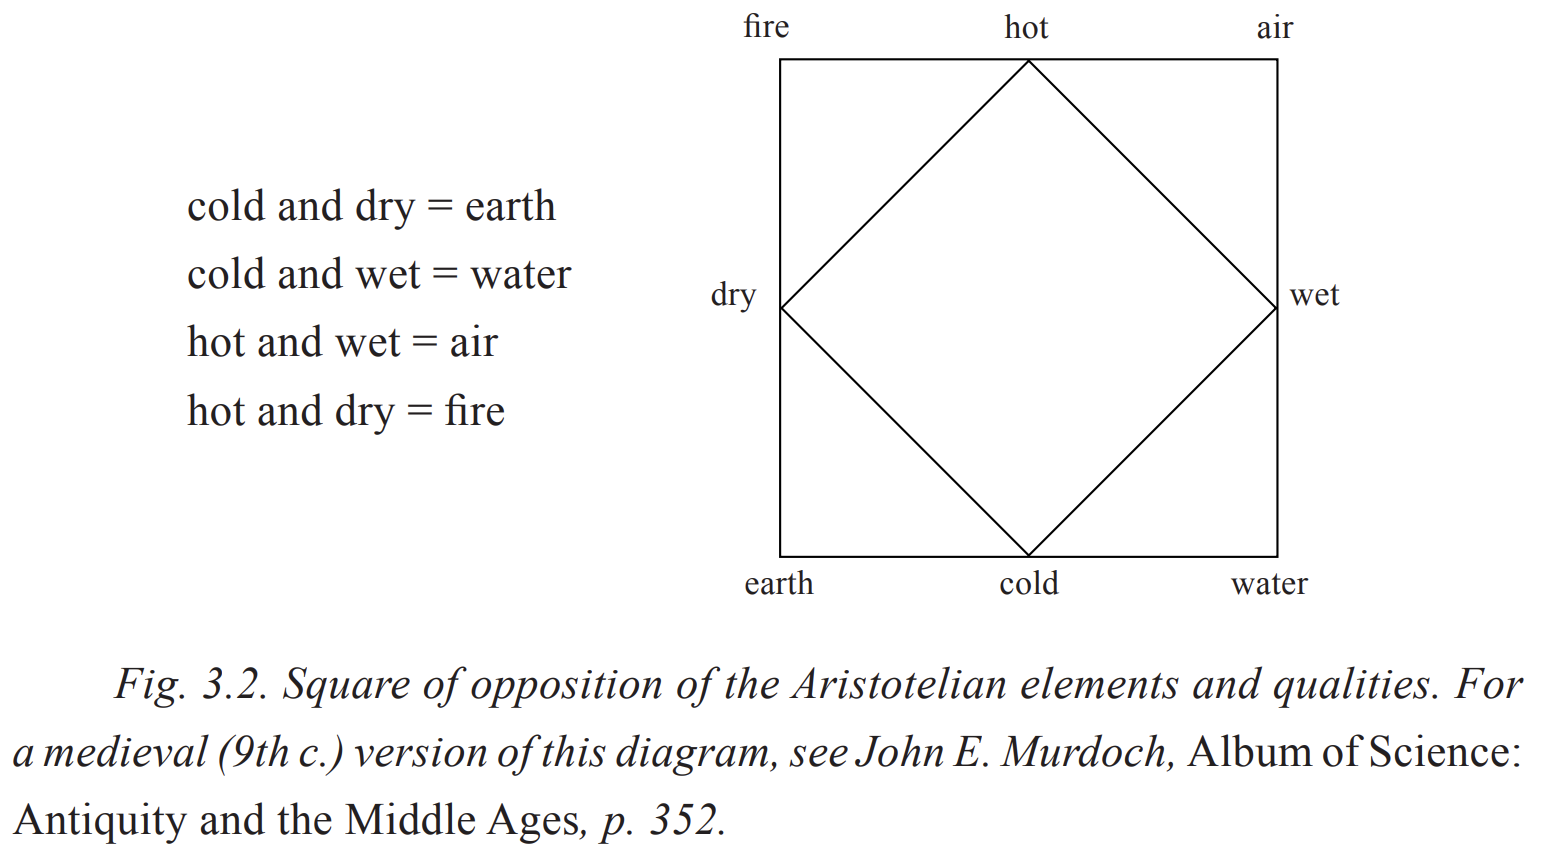
\includegraphics[width=0.75\linewidth]{image/Text2/Fig2.1.png} % 假设图片文件名为fig3.2.jpg,且与.tex文件在同一目录下,如果不在同一目录,需写完整路径

\end{figure}

\noindent26\\
The sublunar region is the scene of generation, corruption, and impermanence. Aristotle, like his predecessors, inquired into the basic element or elements to which the multitude of substances found in the terrestrial region can be reduced. He accepted the four elements originally proposed by Empedocles and subsequently adopted by Plato—earth, water, air, and fire. He agreed with Plato that these elements are in fact reducible to something even more fundamental; but he did not share Plato’s mathematical inclination and therefore refused to accept Plato’s regular solids and their constituent triangles. Instead, he expressed his own commitment to the reality of the world of sense experience by choosing sensible qualities as the ultimate building blocks. Two pairs of qualities are crucial: hot - cold and wet - dry. These combine in four pairs, each of which yields one of the elements (see fig. 3.2). Notice the use made once again of contraries. There is nothing to forbid any of the four qualities being replaced by its contrary, as the result of outside influence. If water is heated, so that the cold of water yields to hot, the water is transformed into air. Such a process easily explains changes of state (from solid to liquid to vapor, and conversely), but also more general transmutation of one substance into another. On such a theory as this, alchemists could easily build.\\
月下区域是生成、腐朽和无常的场所。亚里士多德和他的前辈们一样,探究了地界中众多物质可归结为的一种或几种基本元素。他接受了恩培多克勒最初提出、随后被柏拉图采用的四种元素——土、水、气和火。他同意柏拉图的观点,即这些元素实际上可以归结为更基本的东西;但他没有柏拉图那样的数学倾向,因此拒绝接受柏拉图的正多面体及其构成三角形。相反,他通过选择可感知的性质作为最终的构成要素,表达了自己对感官经验世界真实性的坚持。两对性质至关重要:热 - 冷和湿 - 干。它们以四对的形式组合,每一对产生一种元素(见图3.2)。注意这里再次使用了相反的性质。由于外界影响,没有什么能阻止这四种性质中的任何一种被其相反的性质所取代。如果水被加热,使得水的冷让位于热,水就会变成气。这样一个过程很容易解释状态的变化(从固体到液体再到气体,反之亦然),也能解释一种物质更普遍地转变为另一种物质。炼金术士很容易在这样一种理论基础上进行研究。\\

\noindent27\\
The various substances that make up the cosmos totally fill it, leaving no empty space. To appreciate Aristotle’s view, we must lay aside our almost automatic inclination to think atomistically; we must conceive material things not as aggregates of tiny particles but as continuous wholes. If it is obvious that, say, a loaf of bread is composed of crumbs separated by small spaces, there is no reason not to suppose that those spaces are filled by some finer substance, such as air or water. And there is certainly no simple way of demonstrating, nor indeed any obvious reason for believing, that water and air are anything but continuous. Similar reasoning, applied to the whole of the universe, led Aristotle to the conclusion that the universe is full, a plenum, containing no void space. This claim would be attacked by medieval scholars.\\
构成宇宙的各种物质完全充满了宇宙,没有留下任何空隙。为了理解亚里士多德的观点,我们必须抛开几乎是本能的原子论思维倾向;我们必须把物质事物设想为连续的整体,而不是微小粒子的集合。比如说,一块面包显然是由被小空隙隔开的面包屑组成的,那么没有理由不假定这些空隙被某种更精细的物质,比如空气或水所填满。而且肯定没有简单的方法来证明,实际上也没有任何明显的理由让人相信,水和空气不是连续的。将类似的推理应用于整个宇宙,亚里士多德得出结论,宇宙是充满的,是一个 “充实” 的状态,不存在虚空。这一主张将受到中世纪学者的抨击。\\

\noindent28\\
Aristotle defended this conclusion with a variety of arguments, such as the following. The speed of a falling body is dependent on the density of the medium through which it falls—the less the density, the swifter the motion of the falling body. It follows that in a void space (density zero), there is nothing to slow the descent of the body, from which we would be forced to conclude that the body would fall with infinite speed—a nonsensical notion, since it implies that the body could be at two places at the same time. Critics have frequently noted that this argument can just as well be taken to prove that the absence of resistance does not entail infinite speed as to prove that void does not exist. The point is, of course, well taken. However, we need to understand that Aristotle’s denial of the void did not rest on this single piece of reasoning. In fact, this was but one small part of a lengthy campaign against the atomists, in which Aristotle battled the notion of void space (or void place) with a variety of arguments, some more and some less persuasive.\\
亚里士多德用多种论据来捍卫这一结论,如下所述。一个落体的速度取决于它下落所通过的介质的密度——密度越小,落体的运动就越快。由此可知,在虚空(密度为零)中,没有任何东西能减缓物体的下落,据此我们将不得不得出物体将以无限速度下落的结论——这是一个荒谬的概念,因为这意味着物体可以同时处于两个位置。批评者经常指出,这个论据既可以用来证明没有阻力并不意味着速度无限,也可以用来证明虚空不存在。当然,这一点说得很有道理。然而,我们需要明白,亚里士多德对虚空的否定并不基于这单一的推理。事实上,这只是他反对原子论者的漫长论战中的一小部分,在这场论战中,亚里士多德用各种论据来反驳虚空(或虚空位置)的概念,这些论据有的更有说服力,有的则不那么有说服力。 \\

\noindent29\\
In addition to being hot or cold and wet or dry, each of the elements is also heavy or light. Earth and water are heavy, but earth is the heavier of the two. Air and fire are light, fire being the lighter of the two. In assigning levity to two of the elements, Aristotle did not mean (as we might, if we were making the claim) simply that they are less heavy, but that they are light in an absolute sense; levity is not a weaker version of gravity, but its contrary. Because earth and water are heavy, it is their nature to descend toward the center of the universe; because air and fire are light, it is their nature to ascend toward the periphery (that is, the periphery of the terrestrial region, the spherical shell that contains the moon). If there were no hindrances, therefore, earth and water would collect at the center; because of its greater heaviness, earth would achieve a lower position, forming a sphere at the very center of the universe; water would collect in a concentric spherical shell just outside it. Air and fire naturally ascended, but fire, owing to its greater levity, occupies the outermost region, with air as a concentric sphere just inside it. In the ideal case (in which there are no mixed bodies and nothing prevents the natures of the four elements from fulfilling themselves), the elements would thus form a set of concentric spheres: fire on the outside, followed by air and water, and finally earth at the center (see fig. 3.3). But in reality, the world is composed largely of mixed bodies, one always interfering with another, and the ideal is never attained. Nonetheless, the ideal arrangement defines the natural place of each of the elements; the natural place of earth is at the center of the universe, of fire just inside the sphere of the moon, and so forth.\\
除了热或冷、湿或干之外,每种元素还具有重或轻的属性。土和水是重的,而土是两者中较重的。气和火是轻的,火是两者中较轻的。亚里士多德赋予其中两种元素 “轻性”,他的意思并不是(如果我们提出这样的主张的话可能会认为的那样)仅仅指它们没那么重,而是指它们在绝对意义上是轻的;轻性不是重力的较弱形式,而是它的对立面。因为土和水是重的,它们的本性是向宇宙中心下降;因为气和火是轻的,它们的本性是向周边上升(也就是地界的周边,即包含月球的球壳)。因此,如果没有阻碍,土和水会聚集在中心;由于土更重,它会处于更低的位置,在宇宙的正中心形成一个球体;水会聚集在紧挨着它的一个同心球壳中。气和火自然上升,但由于火更轻,它占据最外层区域,气则作为紧挨着它的一个同心球。在理想情况下(没有混合物体,且没有任何东西阻止四种元素的本性得以实现),这些元素会形成一组同心球:火在最外层,接着是气和水,最后土在中心(见图 3.3)。但在现实中,世界主要由混合物体组成,它们总是相互干扰,理想状态从未达到。尽管如此,这种理想排列定义了每种元素的 “自然位置”;土的自然位置在宇宙中心,火的自然位置在月球球壳内侧,等等。\\

\begin{figure}
    \centering
    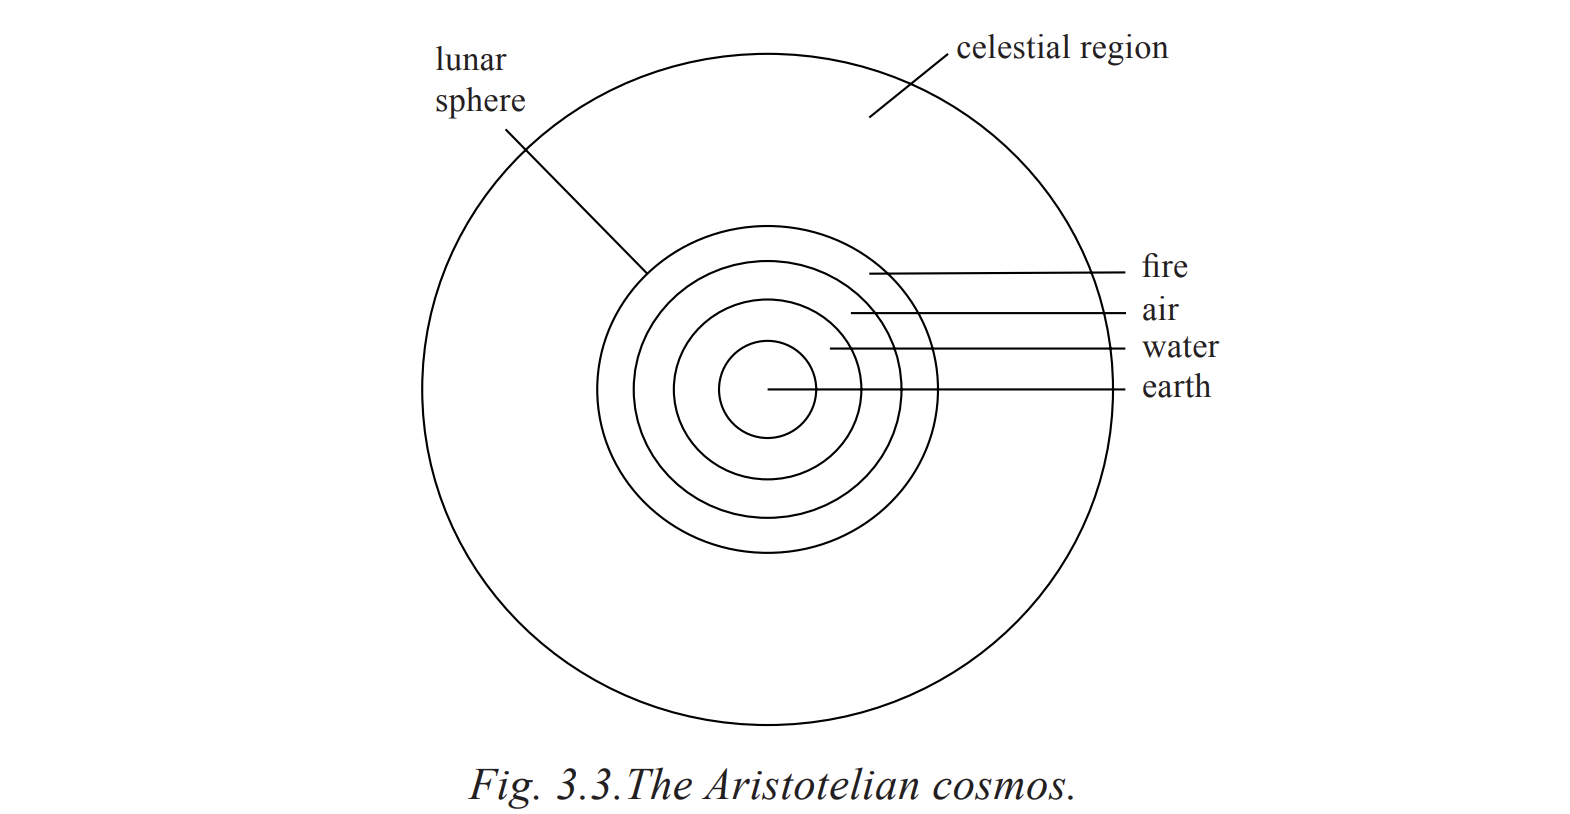
\includegraphics[width=0.75\linewidth]{image/Text2/Fig2.2.png}
\end{figure}

\noindent30\\
It must be emphasized that the arrangement of the elements is spherical. Earth collects at the center to form the earth, and it too is spherical. Aristotle defended this belief with a variety of arguments. Arguing from his natural philosophy, he pointed out that since the natural tendency of earth is to move toward the center of the universe, it must arrange itself symmetrically about that point. But he also called attention to observational evidence, including the circular shadow cast by the earth during a lunar eclipse and the fact that north - south motion by an observer on the surface of the earth alters the apparent position of the stars. Aristotle even reported an estimate by mathematicians of the earth’s circumference (400,000 stades = about 45,000 miles, roughly 1.8 times the modern value). The sphericity of the earth, thus defended by Aristotle, would never be forgotten or seriously questioned. The widespread myth that medieval people believed in a flat earth is of modern origin.\\
必须强调的是,元素的排列是球形的。土聚集在中心形成地球,地球本身也是球形的。亚里士多德用各种论据来捍卫这一观点。从他的自然哲学角度进行论证,他指出,由于土的自然倾向是向宇宙中心移动,它必定会围绕该点对称排列。但他也提请人们注意观测证据,包括月食时地球投射的圆形阴影,以及地球上的观察者进行南北移动时会改变星星的视位置这一事实。亚里士多德甚至提到了数学家对地球周长的估计(400,000斯塔德 = 约45,000英里,大约是现代数值的1.8倍)。亚里士多德如此捍卫的地球球形说,从未被遗忘或受到严重质疑。中世纪人认为地球是平的这一广泛流传的说法是现代才有的误解。 \\

\noindent31\\
Finally, we must note one of the implications of this cosmology, namely that space, instead of being a neutral, homogeneous backdrop (analogous to our modern notion of geometrical space) against which events occur, has properties. Or to express the point more precisely, ours is a world of space, whereas Aristotle’s was a world of place. Heavy bodies move toward their place at the center of the universe not because of a tendency to unite with other heavy bodies located there, but simply because it is their nature to seek that central place; if by some miracle the center happened to be vacant (a physical impossibility in an Aristotelian universe, but an interesting imaginary state of affairs), it would remain the destination of every heavy body.\\
最后,我们必须注意到这种宇宙论的一个含义,即空间并非是事件发生的中性、同质的背景(类似于我们现代的几何空间概念),而是具有属性。或者更精确地表述这一点,我们所处的是一个 “空间的世界”,而亚里士多德的是一个 “位置的世界”。重物向宇宙中心的位置移动,并非因为有与位于那里的其他重物结合的倾向,而仅仅是因为寻求那个中心位置是它们的本性;如果由于某种奇迹,中心碰巧是空的(在亚里士多德的宇宙中这在物理上是不可能的,但却是一种有趣的想象情景),它仍将是每个重物的目的地。\\

\noindent\textbf{Motion, Terrestrial and Celestial 地上与天界的运动}\\
\noindent32\\
We can best understand Aristotle’s theory of motion by grasping its two most fundamental claims. The first is that motion is never spontaneous; there is no motion without a mover. The second is the distinction between two types of motion: motion toward the natural place of the moving body is “natural” motion; motion in any other direction occurs only under coercion from an outside force and is therefore a “forced” or “violent” motion.\\
我们可以通过把握亚里士多德运动理论的两个最基本主张来最好地理解它。第一个主张是,运动绝非自发的;没有推动者就没有运动。第二个主张是区分两种运动类型:朝向运动物体自然位置的运动是 “自然” 运动;在任何其他方向上的运动,只有在受到外力强制时才会发生,因此是 “强制” 或 “暴力” 运动。\\

\noindent33\\
The mover in the case of natural motion is the nature of the body, which is responsible for its tendency to move toward its natural place as defined by the ideal spherical arrangement of the elements. Mixed bodies have a directional tendency that depends on the proportion of the various elements in their composition. When a body undergoing natural motion reaches its natural place, its motion ceases. The mover in the case of forced motion is an external force, which compels the body to violate its natural tendency and move in a direction or manner other than straight - line motion toward its natural place. Such motion ceases when the external force is withdrawn.\\
在自然运动的情况下,推动者是物体的本性,这种本性决定了物体有趋向其由元素的理想球形排列所定义的自然位置的倾向。混合物体具有一种方向性倾向,这取决于其组成中各种元素的比例。当一个进行自然运动的物体到达其自然位置时,它的运动就会停止。在强制运动的情况下,推动者是一种外力,这种外力迫使物体违背其自身的自然倾向,朝着非向其自然位置作直线运动的方向或以非这种方式运动。当外力撤去时,这种运动就会停止。\\

\noindent34\\
So far, this seems sensible. One obvious difficulty, however, is to explain why a projectile hurled horizontally, and therefore undergoing forced motion, does not come to an immediate halt when it loses contact with whatever propelled it. Aristotle’s answer was that the medium takes over as mover. When we project an object, we also act on the surrounding medium (air, for instance), imparting to it the power to move objects; this power is communicated from part to part, in such a way that the projectile is always in contact with a portion of the medium capable of keeping it in motion. If this seems implausible, consider the greater implausibility (from Aristotle’s standpoint) of the alternative—that a projectile, which is inclined by nature to move toward the center of the universe, moves horizontally or upward despite the fact that there is no longer anything causing it to do so.\\
到目前为止,这似乎是合理的。然而,一个明显的难题是解释为什么水平投掷的抛射体,也就是在进行强制运动的物体,在与推动它的物体失去接触后不会立即停止。亚里士多德的答案是,介质接管成为推动者。当我们投掷一个物体时,我们也对周围的介质(例如空气)施加作用,赋予它推动物体的力量;这种力量从一部分传递到另一部分,使得抛射体总是与能够使其保持运动的一部分介质相接触。如果这似乎令人难以置信,那么考虑一下(从亚里士多德的立场来看)另一种情况更令人难以置信——一个本性倾向于向宇宙中心运动的抛射体,却在没有任何东西促使它这样做的情况下水平或向上运动。 \\

\noindent35\\
Force is not the only determinant of motion. In all real cases of motion in the terrestrial realm, there will also be a resistance or opposing force. And it seemed clear to Aristotle that the quickness of motion must depend on these two determining factors—the motive force and the resistance. The question arose: what is the relationship between force, resistance, and speed? Although it probably did not occur to Aristotle that there might be a quantitative law of universal applicability, he was not without interest in the question and did make several forays into quantitative territory. In reference to natural motion in his On the Heavens and again in his Physics, Aristotle claimed that when two bodies of differing weight descend, the times required to cover a given distance will be inversely proportional to the weights. (A body twice as heavy will require half the time). In the same chapter of the Physics, Aristotle introduced resistance into the analysis of natural motion, arguing that if bodies of equal weight move through media of different densities, the times required to traverse a given distance are proportional to the densities of the respective media; that is, the greater the resistance the slower the body moves. Finally, Aristotle also dealt with forced motion in his Physics, claiming that if a given force moves a given weight (against its nature) for a given distance in a given time, the same force will move half that weight twice the distance in that same time (or the same distance in half that time); alternatively, half the force will move half the weight the same distance in the same time.\\
力并非运动的唯一决定因素。在地上领域的所有实际运动情况中,也会存在阻力或反作用力。在亚里士多德看来,运动的快慢显然必定取决于这两个决定因素 —— 动力和阻力。于是问题出现了:力、阻力和速度之间有什么关系呢?尽管亚里士多德可能没有想到会存在一条普遍适用的定量定律,但他对这个问题并非不感兴趣,并且确实对定量领域进行了几次探索。在他的《论天》以及《物理学》中谈及自然运动时,亚里士多德声称,当两个重量不同的物体下落时,经过给定距离所需的时间与重量成反比。(一个重量是另一个两倍的物体所需时间为其一半)。在《物理学》的同一章中,亚里士多德将阻力引入对自然运动的分析,认为如果重量相等的物体在不同密度的介质中运动,经过给定距离所需的时间与各自介质的密度成正比;也就是说,阻力越大,物体运动得越慢。最后,亚里士多德在《物理学》中也探讨了强制运动,声称如果给定的力在给定时间内使给定重量的物体(违背其本性)移动给定距离,那么相同的力在相同时间内将使一半重量的物体移动两倍的距离(或在一半时间内移动相同距离);或者,一半的力将在相同时间内使一半重量的物体移动相同的距离。\\

\noindent36\\
From such statements, some of Aristotle’s successors have made a determined effort to extract a general law. This law is customarily stated as:
\[v\propto F/R\]
That is, velocity ($v$) is proportional to the motive force ($F$) and inversely proportional to the resistance ($R$). For the special case of the natural descent of a heavy body, the motive force is the weight ($W$) of the body, and the relationship then becomes:
\[v\propto W/R\]
Such relationships probably do no great violence to Aristotle’s intent for most cases of motion; however, giving them mathematical form, as we have done, suggests that they hold for all values of $v$, $F$ (or $W$), and $R$—a claim that Aristotle would certainly have denied. He stated explicitly, for example, that a resistance equal to the motive force will prevent motion altogether, whereas the formula above offers no such result. Moreover, the appearance of velocity in these relationships seriously misrepresents Aristotle’s conceptual framework, which contained no concept of velocity as a quantifiable measure of motion, but described motion only in terms of distances and times. Velocity as a technical scientific term to which numerical values might be assigned was a contribution of the Middle Ages (see below, chap. 12).\\
从这些表述中,亚里士多德的一些后继者坚决努力提取出一条普遍定律。这条定律通常表述为:
\[v\propto F/R\]
也就是说,速度($v$)与动力($F$)成正比,与阻力($R$)成反比。对于重物自然下落的特殊情况,动力是物体的重量($W$),那么这种关系就变为:
\[v\propto W/R\]
对于大多数运动情况而言,这样的关系可能并没有严重违背亚里士多德的意图;然而,像我们所做的这样给它们赋予数学形式,意味着它们对$v$、$F$(或$W$)以及$R$的所有值都成立——这是亚里士多德肯定会否认的说法。例如,他明确指出,与动力相等的阻力将完全阻止运动,而上述公式并没有给出这样的结果。此外,速度在这些关系中的出现严重歪曲了亚里士多德的概念框架,他的框架中没有将速度作为运动的可量化度量的概念,而是仅用距离和时间来描述运动。速度作为一个可以赋予数值的技术科学术语,是中世纪的贡献(见下文,第12章)。\\

\noindent37\\
Aristotle has been severely criticized for this theory of motion, on the assumption that any sensible person should have recognized its fatal flaws. Is such criticism justified? In the first place, our goal is to understand the behavior, beliefs, and achievements of historical actors against the background of the culture in which they lived, rather than to assess credit or blame according to the degree to which those historical actors resemble us. In short, historians must always contextualize their subjects. Second, some of the criticisms of Aristotle’s theories of motion apply only to theories foisted onto Aristotle by followers and critics, rather than to his own. Third, the theory in its genuinely Aristotelian (and properly contextualized) version makes quite good sense today and would surely have made good sense in the fourth century B.C. For example, various surveys have shown that the majority of modern, university - educated people are prepared to assent to many of the basics of Aristotle’s theory of motion. Fourth, the relatively modest level of quantitative content in Aristotle’s theory is easily explained as the outcome of his larger philosophy of nature. His primary goal was to understand essential natures, not to explore quantitative relationships between such incidental factors as the space - time (or place - time) coordinates applicable to a moving body; even an exhaustive investigation of the latter gives us no useful information about the former. You may criticize Aristotle, if you like, for not being interested in whatever interests modern scientists, but we do not thereby learn anything significant about Aristotle.\\
亚里士多德因其运动理论而受到严厉批评,人们假定任何明智的人都应该认识到它的致命缺陷。这样的批评合理吗?首先,我们的目标是在历史人物所处的文化背景下理解他们的行为、信仰和成就,而不是根据这些历史人物与我们的相似程度来评定功过。简而言之,历史学家必须始终将他们的研究对象置于特定背景中。其次,对亚里士多德运动理论的一些批评仅适用于追随者和批评者强加给他的理论,而不适用于他自己的理论。第三,真正属于亚里士多德(且置于适当背景中)的理论版本在今天相当有道理,在公元前 4 世纪肯定也很有道理。例如,各种调查表明,大多数受过大学教育的现代人愿意认可亚里士多德运动理论的许多基本观点。第四,亚里士多德理论中相对较少的定量内容很容易解释为他更大的自然哲学的结果。他的主要目标是理解本质,而不是探索诸如适用于运动物体的时空(或位置 - 时间)坐标等偶然因素之间的定量关系;即使对后者进行详尽的研究,也不会为我们提供关于前者的有用信息。如果你愿意,你可以批评亚里士多德对现代科学家感兴趣的东西不感兴趣,但我们并不会因此对亚里士多德有任何重要的了解。\\

\noindent38\\
Motion in the celestial sphere is an altogether different sort of phenomenon. The heavens, composed of the incorruptible quintessence, possess no contraries and are therefore incapable of qualitative change. It might seem fitting for such a region to be absolutely motionless, but this hypothesis is defeated by the most casual observation of the heavens. Aristotle therefore assigned to the heavens the most perfect of motions—continuous uniform circular motion. Besides being the most perfect of motions, uniform circular motion appears to have the capability of explaining the observed celestial cycles.\\
天界的运动是一种完全不同的现象。天界由不可腐朽的以太构成,没有相反的性质,因此不会发生性质上的变化。对于这样一个区域来说,似乎完全静止是合适的,但这种假设被对天界最粗略的观察所否定。因此,亚里士多德赋予天界最完美的运动 —— 连续匀速圆周运动。匀速圆周运动除了是最完美的运动之外,似乎还有能力解释所观测到的天体循环现象。\\

\noindent39\\
By Aristotle’s day, these cycles had been an object of study for centuries in the Greek world and for millennia in its predecessor civilizations. It was understood that the “fixed” stars move with perfect uniformity, as though fixed to a uniformly rotating sphere, with a period of rotation of approximately one day. But there were seven stars, the wandering stars or planets, that displayed a more intricate motion, apparently crawling around on the stellar sphere as it went through its daily rotation. These seven were the Sun, Moon, Mercury, Venus, Mars, Jupiter, and Saturn. The sun crawls slowly (about 1°/day), west to east with small variations in speed, through the sphere of fixed stars along a path called the ecliptic, which passes through the center of the zodiac [...]. The moon follows approximately the same course, but at the more rapid rate of about 12°/day. The remaining planets also move along the ecliptic (or in its vicinity) with variable speed and with an occasional reversal of direction.\\
在亚里士多德的时代,这些循环现象在希腊世界已被研究了数个世纪,在其之前的文明中更是被研究了数千年。人们知道 “恒星” 以完美的均匀性运动,仿佛固定在一个匀速旋转的球体上,旋转周期约为一天。但有七颗星,即 “漫游的星” 或行星,展现出更为复杂的运动,在恒星天球进行每日旋转时,它们似乎在天球上四处 “爬行”。这七颗星是太阳、月亮、水星、金星、火星、木星和土星。太阳缓慢地(约每天 1°)自西向东移动,速度有微小变化,沿着一条称为黄道的路径穿过恒星天球,黄道经过黄道十二宫的中心 [...]。月亮大致沿着相同的路径运行,但速度更快,约为每天 12°。其余的行星也沿着黄道(或在其附近)以变化的速度移动,偶尔还会改变方向。\\

\noindent40\\
Are such complex motions compatible with the requirement of uniform circular motion in the heavens? Eudoxus, a generation before Aristotle, had already shown that they are. I will return to this subject in chap. 5; for the moment, it will be sufficient to point out that Eudoxus treated each complex planetary motion as a composite of a series of simple uniform circular movements. He did this by assigning to each planet a set of concentric spheres, and to each sphere one component of the complex planetary motion. Aristotle took over this scheme, with various modifications. When he was finished, he had produced an intricate piece of celestial machinery, consisting of fifty - five planetary spheres plus the sphere of the fixed stars.\\
如此复杂的运动与天界匀速圆周运动的要求是否相符呢?比亚里士多德早一代的欧多克斯已经证明它们是相符的。我将在第五章回到这个主题;目前,指出欧多克斯把每一种复杂的行星运动都视为一系列简单匀速圆周运动的组合就足够了。他通过给每颗行星分配一组同心球,并给每个球赋予复杂行星运动的一个分量来做到这一点。亚里士多德采用了这个方案,并做了各种修改。当他完成时,他构建出了一套复杂的天体机制,由五十五个行星天球加上恒星天球组成。\\

\noindent41\\
What is the cause of movement in the heavens? Aristotle’s natural philosophy would not allow such a question to go unasked. The celestial spheres are composed, of course, of the quintessence; their motion, being eternal, must be natural rather than forced. The cause of this eternal motion must itself be unmoved, for if we do not postulate an unmoved mover, we quickly find ourselves trapped in an infinite regress: a moving mover must have acquired its motion from yet another moving mover, and so on. Aristotle identified the unmoved mover for the planetary spheres as the “Prime Mover,” a living deity representing the highest good, wholly actualized, totally absorbed in self - contemplation, nonspatial, separated from the spheres it (or he or she) moves, and not at all like the traditional anthropomorphic Greek gods. How, then, does the Prime Mover or Unmoved Mover cause motion in the heavens? Not as efficient cause, for that would require contact between the mover and the moved, but as final cause. That is, the Prime Mover is the object of desire for the celestial spheres, which endeavor to imitate its changeless perfection by assuming eternal, uniform circular motions. Any reader who has followed this much of Aristotle’s discussion would be justified in assuming that there is a single Unmoved Mover for the entire cosmos; it comes as something of a surprise, therefore, when Aristotle announces that, in fact, each of the celestial spheres has its own Unmoved Mover, the object of its affection and the final cause of its motion.\\
天界运动的原因是什么?亚里士多德的自然哲学不会允许这样的问题不被提出。天球当然是由以太构成的;它们的运动是永恒的,必然是自然的而非强制的。这种永恒运动的原因自身必定是不动的,因为如果我们不假定一个不动的推动者,我们很快就会发现自己陷入无穷回溯:一个运动的推动者必定是从另一个运动的推动者那里获得其运动的,如此等等。亚里士多德把行星天球的不动推动者确定为 “第一推动者”,这是一个代表最高善的有生命的神,完全实现了自身,全神贯注于自我沉思,没有空间性,与它(或他或她)所推动的天球相分离,一点也不像传统的拟人化的希腊诸神。那么,第一推动者或不动推动者是如何导致天界运动的呢?不是作为动力因,因为那将需要推动者和被推动者之间的接触,而是作为目的因。也就是说,第一推动者是天球渴望的对象,天球通过采取永恒、匀速的圆周运动来努力模仿它不变的完美。任何跟随亚里士多德进行到这里讨论的读者都会有理由假定整个宇宙有一个单一的不动推动者;因此,当亚里士多德宣布事实上每个天球都有自己的不动推动者,即它爱慕的对象和其运动的目的因时,这多少有些令人惊讶。\\

\noindent42\\


\noindent43\\


\noindent44\\


\noindent45\\


\noindent46\\


\noindent47\\


\noindent48\\


\noindent49\\


\noindent50\\


\noindent51\\


\noindent52\\


\noindent53\\


\noindent54\\


\noindent55\\





\newpage

\section{Text 3a from The Birth of a New Physics/ \textit{I. Bernard Cohen}}
\begin{center}
CHAPTER 7 第三章\\
The Grand Design — A New Physics\\
\end{center}
\noindent1\\
The publication of Isaac Newton’s \textit{Principia} in 1687 was one of the most notable events in the whole history of physical science. In it one may find the culmination of thousands of years of striving to comprehend the system of the world, the principles of force and of motion, and the physics of bodies moving in different media. It is no small testimony to the vitality of Newton’s scientific genius that although the physics of the \textit{Principia} has been altered, improved, and challenged ever since, we still set about solving most problems of celestial mechanics and the physics of gross bodies by proceeding essentially as Newton did some 300 years ago. Newtonian principles of celestial mechanics guide our artificial satellites, our space shuttles, and every spacecraft we launch to explore the vast reaches of our solar system. And if this is not enough to satisfy the canons of greatness, Newton was equally great as a pure mathematician. He invented the differential and integral calculus (produced simultaneously and independently by the German philosopher Gottfried Wilhelm Leibniz), which is the language of physics; he developed the binomial theorem and various properties of infinite series; and he laid the foundations for the calculus of variations. In optics, Newton began the experimental study of the analysis and composition of light, showing that white light is a mixture of light of many colors, each having a characteristic index of refraction. Upon these researches have risen the science of spectroscopy and the methods of color analysis. Newton invented a reflecting telescope and so showed astronomers how to transcend the limitations of telescopes built of lenses. All in all, his was a fantastic scientific achievement—of a kind that has never been equaled and may never be equaled again.\\
1687年,艾萨克·牛顿的《自然哲学的数学原理》的出版,是整个物理科学史上最引人注目的事件之一。在这本书中,可以看到数千年来人们为理解世界体系、力和运动原理以及在不同介质中运动的物体的物理学所付出努力的顶峰。尽管自那以后,《自然哲学的数学原理》中的物理学理论已经被修改、完善和挑战,但我们仍然基本上按照牛顿在约300年前的方法来解决大多数天体力学和宏观物体物理学的问题,这充分证明了牛顿科学天赋的生命力。牛顿的天体力学原理指导着我们的人造卫星、航天飞机以及我们发射的每一艘探索太阳系广阔区域的宇宙飞船。如果这还不足以满足伟大的标准,那么牛顿作为一名纯粹的数学家同样伟大。他发明了微积分(与德国哲学家戈特弗里德·威廉·莱布尼茨同时且独立地提出),而微积分是物理学的语言;他发展了二项式定理以及无穷级数的各种性质;他为变分法奠定了基础。在光学方面,牛顿开启了对光的分析和合成的实验研究,表明白光 是许多颜色的光的混合,每种颜色都有其特征折射率。基于这些研究,光谱学和颜色分析方法得以发展。牛顿发明了反射望远镜,从而向天文学家展示了如何超越透镜望远镜的局限性。总而言之,他取得了非凡的科学成就——这种成就前无古人,或许也后无来者。 \\

\noindent2\\
In this book we shall deal exclusively with Newton’s system of dynamics and gravitation, the central problems for which the preceding chapters have been a preparation. If you have read them carefully, you have in mind all but one of the major ingredients requisite to an understanding of the Newtonian system of the world. But even if that one were to be given—the analysis of uniform circular motion—the guiding hand of Newton would still be required to put the ingredients together. It took genius to supply the new concept of universal gravitation. Let us see what Newton actually did.\\
在本书中,我们将专门探讨牛顿的动力学和引力体系,前面的章节就是为这些核心问题做铺垫的。如果你仔细读过前面的章节,那么对于理解牛顿的世界体系所需的主要要素,除了一个之外,你都已心中有数。但即便给出了这一个要素——匀速圆周运动的分析——仍需要牛顿的指引才能将这些要素整合起来。提出万有引力这一新概念需要天赋。让我们看看牛顿实际上做了什么。\\

\noindent3\\
First of all, it must be understood that Galileo himself never attempted to display any scheme of forces that would account for the movement of the planets, or of their satellites. As for Copernicus, the \textit{De revolutionibus} contains no important insight into a celestial mechanics. Kepler had tried to supply a celestial mechanism, but the result was never a very happy one. He held that the \textit{anima motrix} emanating from the sun would cause planets to revolve about the sun in circles. He further supposed that magnetic interactions of the sun and a planet would shift the planet during an otherwise circular revolution into an elliptical orbit. Others who contemplated the problems of planetary motion proposed systems of mechanics containing certain features that were later to appear in Newtonian dynamics. One of these was Robert Hooke, who quite understandably thought that Newton should have given him more credit than a mere passing reference for having anticipated parts of the laws of dynamics and gravitation.\\
首先,必须明白的是,伽利略本人从未试图展示任何能够解释行星或其卫星运动的力的方案。至于哥白尼,《天体运行论》(\textit{De revolutionibus}) 对天体力学没有重要的见解。开普勒曾试图提供一种天体机制,但结果并不理想。他认为,从太阳发出的 “动力精灵”(\textit{anima motrix})会使行星绕太阳做圆周运动。他进一步推测,太阳和行星之间的磁相互作用会在原本的圆周运动中使行星进入椭圆轨道。其他思考行星运动问题的人提出了一些力学体系,其中包含了后来出现在牛顿动力学中的某些特征。其中之一是罗伯特·胡克,他认为牛顿本应为他预见到动力学和引力定律的部分内容而给予他比仅仅一笔带过更多的认可,这是可以理解的。\\

\noindent\textbf{Newtonian Anticipations}\\
\noindent4\\
The climactic chapter in the discovery of the mechanics of the universe starts with a pretty story. By the third quarter of the seventeenth century, a group of men had become so eager to advance the new mathematical experimental sciences that they banded together to perform experiments in concert, to present problems for solution to one another, and to report on their own researches and on those of others as revealed by correspondence, books, and pamphlets. Thus it came about that Robert Hooke, Edmond Halley, and Sir Christopher Wren, England’s foremost architect, met to discuss the question, Under what law of force would a planet follow an elliptical orbit? From Kepler’s laws—especially the third or harmonic law, but also the second or law of areas—it was clear that the sun somehow or other must control or at least affect the motion of a planet in accordance with the relative proximity of the planet to the sun. Even if the particular mechanisms proposed by Kepler (an \textit{anima motrix} and a magnetic force) had to be rejected, there could be no doubt that some kind of planet - sun interaction keeps the planets in their courses. Furthermore, a more acute intuition than Kepler’s would sense that any force emanating from the sun must spread out in all directions from that body, presumably diminishing according to the inverse of the square of its distance from the sun—as the intensity of light diminishes in relation to distance. But to say this much is a very different thing from proving it mathematically. For to prove it would require a complete physics with mathematical methods for solving all the attendant and consequent problems. When Newton declined to credit authors who tossed off general statements without being able to prove them mathematically or fit them into a valid framework of dynamics, he was quite justified in saying, as he did of Hooke’s claims: “Now is not this very fine? Mathematicians that find out, settle, and do all the business must content themselves with being nothing but dry calculators and drudges; and another, that does nothing but pretend and grasp at all things, must carry away all the invention, as well of those that were to follow him as of those that went before.” (See, further, Supplement 11).\\
宇宙力学发现历程中的高潮篇章始于一个有趣的故事。到17世纪的第三个25年,一群人如此热衷于推进新的数学实验科学,以至于他们联合起来协同进行实验,相互提出问题以求解答,并就自己的研究以及通过通信、书籍和小册子所了解到的他人研究进行汇报。于是,罗伯特·胡克、埃德蒙·哈雷以及英国最杰出的建筑师克里斯托弗·雷恩爵士会面,讨论这样一个问题:在何种力的定律下,行星会沿椭圆轨道运行?从开普勒定律——尤其是第三定律(调和定律),但也包括第二定律(面积定律)——可以明显看出,太阳以某种方式必定控制或至少影响着行星的运动,这种影响与行星和太阳的相对距离有关。即使开普勒提出的特定机制(一种 “动力精灵” 和磁力)必须被摒弃,但毫无疑问,某种行星 - 太阳间的相互作用使行星保持在其轨道上。此外,比开普勒更敏锐的直觉会意识到,任何从太阳发出的力必定从太阳向各个方向传播,大概会按照与太阳距离的平方反比而减弱——就像光的强度随距离减弱一样。但仅仅这么说与用数学方法证明它是截然不同的两回事。因为要证明它,就需要一门完整的物理学,具备用数学方法解决所有相关和随之而来问题的能力。当牛顿拒绝认可那些随口抛出一般性陈述却无法用数学方法证明或无法将其纳入有效动力学框架的作者时,他在评价胡克的主张时所说的话是完全合理的:“这不是很棒吗?那些发现、确定并完成所有工作的数学家,只能满足于仅仅成为枯燥的计算者和苦工;而另一个人,除了装模作样、妄图抓住一切之外什么都不做,却必须把所有的发明成果都据为己有,包括那些后来者和先行者的成果。”(另见补编11) \\

\noindent5\\
In any event, by January 1684 Halley had concluded that the force acting on planets to keep them in their orbits “decreased in the proportion of the squares of the distances reciprocally,” 
\[F\propto\frac{1}{D^{2}}\]
but he was not able to deduce from that hypothesis the observed motions of the celestial bodies. When Wren and Hooke met later in the month, they agreed with Halley’s supposition of a solar force. Hooke boasted “that upon that principle all the laws of the celestial motions were to be [i.e., could be] demonstrated, that he himself had done it.” But despite repeated urgings and Wren’s offer of a considerable monetary prize, Hooke did not—and presumably could not—produce a solution. Six months later, in August 1684, Halley decided to go to Cambridge to consult Isaac Newton. On his arrival he learned the “good news” that Newton “had brought this demonstration to perfection.” Here is DeMoivre’s almost contemporaneous account of that visit:\\
After they had been some time together, the Dr. [Halley] asked him what he thought the curve would be that would be described by the planets supposing the force of attraction towards the sun to be reciprocal to the square of their distance from it. Sir Isaac replied immediately that it would be an ellipsis. The Doctor, struck with joy and amazement, asked him how he knew it. Why, saith he, I have calculated it. Whereupon Dr. Halley asked him for his calculation without any further delay. Sir Isaac looked among his papers but could not find it, but he promised him to renew it and then to send it him. Sir Isaac, in order to make good his promise, fell to work again, but he could not come to that conclusion which he thought he had before examined with care. However, he attempted a new way which, though longer than the first, brought him again to his former conclusion. Then he examined carefully what might be the reason why the calculation he had undertaken before did not prove right, and he found that, having drawn an ellipsis coarsely with his own hand, he had drawn the two axes of the curve, instead of drawing two diameters somewhat inclined to one another, whereby he might have fixed his imagination to any two conjugate diameters, which was requisite he should do. That being perceived, he made both his calculations agree together.\\
无论如何,到1684年1月,哈雷得出结论,使行星保持在其轨道上的力 “与距离的平方成反比减小”,即:
\[F\propto\frac{1}{D^{2}}\]
但他无法从这个假设中推导出所观测到的天体运动。当月晚些时候,雷恩和胡克会面时,他们认同哈雷关于太阳力的假设。胡克吹嘘说 “基于那个原理,所有天体运动定律都可以(即能够)被证明,而且他自己已经做到了”。但尽管反复催促,并且雷恩提供了一笔可观的奖金,胡克却没有——大概也无法——给出一个解决方案。六个月后,即1684年8月,哈雷决定前往剑桥咨询艾萨克·牛顿。他一到那里就得知了 “好消息”,即牛顿 “已经完善了这个证明”。以下是棣莫弗几乎同时代对那次访问的描述:

\addtolength{\leftskip}{1cm}
他们在一起待了一段时间后,(哈雷)博士问他,假设行星受到的朝向太阳的引力与它们和太阳距离的平方成反比,他认为行星将描绘出什么样的曲线。艾萨克爵士立刻回答说那将是一个椭圆。博士既高兴又惊讶,问他是怎么知道的。他说,“哎呀,我算过了。” 于是哈雷博士毫不迟疑地向他索要计算过程。艾萨克爵士在他的论文中找了找,但没有找到,不过他答应重新计算然后寄给他。为了履行诺言,艾萨克爵士又开始工作,但他无法得出他之前认为已经仔细研究过的那个结论。然而,他尝试了一种新方法,虽然比第一种方法长,但又让他得出了之前的结论。然后他仔细检查了之前计算不正确的原因,他发现,由于他自己粗略地画了一个椭圆,他画的是曲线的两条轴,而不是两条相互有点倾斜的直径,而他本应该把注意力集中在任意两条共轭直径上。意识到这一点后,他使两次计算结果相符了。 \\

\addtolength{\leftskip}{-1cm}

\noindent6\\
Spurred on by Halley’s visit, Newton resumed work on a subject that had commanded his attention in his twenties when he had laid the foundations of his other great scientific discoveries: the nature of white light and color and the differential and integral calculus. He now put his investigations in order, made great progress, and in the fall term of the year, discussed his research in a series of lectures on dynamics that he gave at Cambridge University, as required by his professorship. Eventually, with Halley’s encouragement, a draft of these lectures, \textit{De motu corporum}, grew into one of the greatest and most influential books any man has yet conceived. Many a scientist has echoed the sentiment that Halley expressed in the ode he wrote as a preface to Newton’s \textit{Principia} (or, to give Newton’s masterpiece its full title, \textit{Philosophiae naturalis principia mathematica, Mathematical Principles of Natural Philosophy}, London, 1687):\\

\addtolength{\leftskip}{1cm}
\noindent\textit{
Then ye who now on heavenly nectar fare,\\
Come celebrate with me in song the name\\
Of Newton, to the Muses dear; for he\\
Unlocked the hidden treasuries of Truth:\\
So richly through his mind had Phoebus cast\\
The radiance of his own divinity.\\
Nearer the gods no mortal may approach.\\}

\addtolength{\leftskip}{-1cm}

\noindent 在哈雷访问的激励下,牛顿重新开始研究一个在他二十多岁时就引起他关注的课题,那时他奠定了其他重大科学发现的基础:白光和颜色的本质以及微积分。他现在整理了自己的研究,取得了很大进展,并在当年秋季学期,按照教授职位的要求,在剑桥大学的一系列动力学讲座中讨论了他的研究。最终,在哈雷的鼓励下,这些讲座的草稿《论物体的运动》(拉丁文为“\textit{De motu corporum}”)发展成为有史以来最伟大、最具影响力的著作之一。许多科学家都对哈雷在为牛顿的《自然哲学的数学原理》(或者,完整地说出牛顿这部杰作的书名,即 1687 年于伦敦出版的《自然哲学的数学原理》,拉丁文为 “\textit{Philosophiae naturalis principia mathematica}” )所写的序诗中表达的情感表示赞同:\\

\addtolength{\leftskip}{1cm}

\noindent 你们这些如今享用天国琼浆的人啊,\\
来和我一起用歌声颂扬\\
牛顿的名字吧,他受缪斯女神钟爱;因为他\\
开启了真理隐藏的宝库:\\
太阳神已如此丰富地将\\
他自身神性的光辉投射进牛顿的脑海。\\
凡人再也无法更接近诸神。 \\

\addtolength{\leftskip}{-1cm}

\noindent\textbf{The Principia}\\
\noindent7\\
The \textit{Principia} is divided into three parts or books; we shall concentrate on the first and third. In Book One Newton develops the general principles of the dynamics of moving bodies, and in Book Three he applies the principles to the mechanism of the universe. Book Two deals with a facet of fluid mechanics, the theory of waves, and other aspects of physics.\\
《自然哲学的数学原理》分为三个部分或三卷;我们将专注于第一卷和第三卷。在第一卷中,牛顿阐述了运动物体动力学的一般原理,在第三卷中,他将这些原理应用于宇宙的机制。第二卷涉及流体力学的一个方面、波动理论以及物理学的其他方面。 \\

\noindent8\\
In Book One, following the preface, a set of definitions, and a discussion of the nature of time and space, Newton presented the ``axioms, or laws of motion'':

\noindent 运动的变化与施加的力成正比,并沿着该力施加的直线方向发生。[参见第184页的补充说明。]
在第一册中,在前言之后,牛顿提出了一系列定义,并对时间和空间的性质进行了讨论,然后提出了“公理或运动定律”:

\addtolength{\leftskip}{1cm}
\addtolength{\rightskip}{1cm}

\begin{center}
\noindent\textbf\textit{Law I 第一定律}
\end{center}
\noindent Every body perseveres in its state of being at rest or of moving uniformly straight forward, except insofar as it is compelled to change its state by forces impressed upon it.\\
每个物体都保持其静止或匀速直线运动的状态,除非它受到外力作用而被迫改变这种状态。\\

\begin{center}
\noindent\textbf\textit{Law II 第二定律}
\end{center}
\noindent A change in motion is proportional to the motive force impressed and takes place in the direction of the straight line along which that force is impressed. [See Suppl. Note on p. 184.]\\
运动的变化与施加的力成正比,并沿着该力施加的直线方向发生。[参见第184页的补充说明。]\\

\addtolength{\leftskip}{-1cm}
\addtolength{\rightskip}{-1cm}

\noindent9\\
Observe that if a body is in uniform motion in a straight line, a force at right angles to the direction of motion of the body will not affect the forward motion. This follows from the fact that the acceleration is always in the same direction as the force producing it, so that the acceleration in this case is at right angles to the direction of motion. Thus in the toy train experiment of Chapter 5, the chief force acting is the downward force of gravity, producing a vertical acceleration. The ball, whether moving forward or at rest, is thus caused to slow down in its upward motion until it comes to rest, and then be speeded up or accelerated on the way down.\\
观察到,如果一个物体在直线上做匀速运动,一个与物体运动方向成直角的力不会影响其向前的运动。这是由于加速度总是与产生它的力的方向相同,因此这种情况下的加速度与运动方向成直角。因此在第五章的玩具火车实验中,主要作用力是向下的重力,产生垂直加速度。球无论是向前移动还是静止,都会在向上运动时减速直到停止,然后在下降过程中加速或加速。\\

\noindent10\\
A comparison of the two sets of photographs (p. 83) shows that the upward and downward motions are exactly the same whether the train is at rest or in uniform motion. In the forward direction there is no effect of weight or gravity, since this acts only in a downward direction. The only force in the forward or horizontal direction is the small amount of air friction, which is almost negligible; so one may say that in the horizontal direction there is no force acting. According to Newton's first law of motion, the ball will continue to move in the forward direction with uniform motion in a straight line just as the train does—a fact you can check by inspecting the photograph. The ball remains above the locomotive whether the train is at rest or in uniform motion in a straight line. This law of motion is sometimes called the principle of inertia, and the property that material bodies have of continuing in a state of rest or uniform motion in a straight line is sometimes known as the bodies' \textit{inertia}\footnote{The earliest known statement of this law was made by René Descartes in a book that he did not publish. It appeared in print for the first time in a work by Pierre Gassendi. But prior to Newton's \textit{Principia} there was no completely developed inertial physics. It is not without significance that this early book of Descartes was based on the Copernican point of view; Descartes suppressed it on learning of the condemnation of Galileo. Gassendi likewise was a Copernican. He actually made experiments with objects let fall from moving ships and moving carriages to test Galileo's conclusions about inertial motion. Descartes first published his version of the law of inertia in his \textit{Principles of Philosophy} (1644); the earlier statement, in Descartes's \textit{The World}, was published after Descartes's death in 1650. See Suppl. 8.}.\\
对两组照片(第83页)的比较表明,无论火车是静止还是做匀速直线运动,向上和向下的运动完全相同。在前进方向上,重量或重力没有影响,因为这仅在向下方向起作用。前进或水平方向上的唯一力是几乎可以忽略不计的空气阻力;因此可以说在水平方向上没有力作用。根据牛顿第一运动定律,球将继续以匀速直线运动的方式前进,就像火车一样——这一事实你可以通过检查照片来验证。无论火车是静止还是做匀速直线运动,球都保持在火车上方。这一运动定律有时被称为惯性原理,而物体保持静止状态或匀速直线运动状态的性质有时被称为物体的惯性\footnote{这一定律的最早陈述是由勒内·笛卡尔在一本他未出版的书中提出的。它首次出现在皮埃尔·伽桑迪的作品中。但在牛顿的《自然哲学的数学原理》之前,还没有完全发展的惯性物理学。笛卡尔的早期著作基于哥白尼白尼点的视角这一点并非没有意义;笛卡尔在得知伽利略被谴责后压制了它。伽桑迪同样是哥白尼点主义者。他实际上用从移动的船只和移动的马车上掉落的物体进行实验,以测试伽利略关于惯性运动的结论。笛卡尔在他的《哲学原理》(1644年)中首次发表了惯性定律的版本;笛卡尔在《世界》中的早期陈述是在笛卡尔去世后的1650年出版的。参见补充8。}。\\

\noindent11\\
Newton illustrated Law I by reference to projectiles that continue in their forward motions ``so far as they are not retarded by the resistance of the air, or impelled downward by the force of gravity,'' and he referred also to ``the greater bodies of planets and comets.'' (On the inertial aspect of the motion of ``greater bodies'' such as ``planets and comets,'' see Supplement 12.) At this one stroke Newton postulated the opposite view of Aristotelian physics. In the latter, no celestial body could move uniformly in a straight line in the absence of a force, because this would be a ``violent'' motion and so contrary to its nature. Nor could a terrestrial object, as we have seen, move along its ``natural'' straight line without an external mover or an internal motive force. Newton, presenting a physics that applies simultaneously to both terrestrial and celestial objects, stated that in the absence of a force bodies do not necessarily stand still or come to rest as Aristotle supposed, but they may move at constant rectilinear speed. This ``indifference'' of all sorts of bodies to rest or uniform straight-line motion in the absence of a force clearly is an advanced form of Galileo's statement in his book on sunspots (p. 88), the difference being that in that work Galileo was writing about uniform motion along a great spherical surface concentric with the earth.\\
牛顿通过引用在“空气阻力不减慢它们,或重力不使它们下落”的情况下继续前进的抛射物来说明第一定律,他还提到了“较大的天体,如行星和彗星”。(关于“较大天体”如“行星和彗星”的运动惯性方面,参见补充12。)牛顿在此一举提出了与亚里士多德物理学相反的观点。在后者中,没有天体可以在没有力的情况下沿直线做匀速运动,因为这将是一种“暴力”运动,与其本性相反。正如我们所见,地面物体也不能在没有外部推动者或内部动力的情况下沿其“自然”直线运动。牛顿提出了一种同时适用于地面和天体的物理学,他指出在没有力的情况下,物体不一定像亚里士多德所认为的那样静止或停止,但它们可以以恒定的直线速度运动。这种在没有力的情况下对所有物体静止或匀速直线运动的“冷漠”显然是伽利略在其关于太阳黑子的书中陈述(第88页)的高级形式,不同之处在于在那项工作中伽利略是在写关于沿与地球同心的大球面做匀速运动。\\

\noindent12\\
Newton said of the laws of motion that they were ``such principles as have been received by mathematicians, and \ldots confirmed by [an] abundance of experiments. By the first two Laws and the first two Corollaries, Galileo discovered that the descent of bodies varies as the square of the time and that the motion of projectiles is in the curve of a parabola, experience agreeing with both, unless so far as these motions are a little retarded by the resistance of the air.'' The ``two Corollaries'' deal with methods used by Galileo and many of his predecessors to combine two different forces or two independent motions. Fifty years after the publication of Galileo's \textit{Two New Sciences} it was difficult for Newton, who had already established an inertial physics, to conceive that Galileo could have come as close as he had to the concept of inertia without having taken full leave of circularity and having known the true principle of linear inertia.\\
牛顿谈到运动定律时说,它们是“已被数学家接受的这样的原理,并且……通过[大量]实验得到证实。通过前两条定律和前两个推论,伽利略发现物体的下落速度与时间的平方成正比,抛射体的运动轨迹是抛物线,经验与两者都相符,除非这些运动因空气阻力而稍有减慢。” “两个推论”涉及伽利略及其许多前辈用来结合两种不同力或两种独立运动的方法。在伽利略的《两门新科学》出版五十年后,对于已经建立了惯性物理学的牛顿来说,很难想象伽利略在没有完全摆脱圆周运动并且了解真正的线性惯性原理的情况下,能够如此接近惯性概念。\\

\noindent13\\
Newton was being very generous to Galileo because, however it may be argued that Galileo ``really did'' have the law of inertia or Newton's Law I, a great stretch of the imagination is required to assign any credit to Galileo for Law II. This law has two parts. In the second half of Newton's statement of Law II, the ``change in motion'' produced by an ``impressed'' or ``motive'' force—whether that is a change in the speed with which a body moves or a change in the direction in which it is moving—is said to be ``in the direction of the straight line along which that force is impressed.'' This much is certainly implied in Galileo's analysis of projectile motion because Galileo assumed that in the forward direction there is no acceleration because there is no horizontal force, except the negligible action of air friction; but in the vertical direction there is an acceleration or continual increase of downward speed, because of the downward-acting weight force. But the first part of Law II—that the change in the magnitude of the motion is related to the motive force—is something else again; only a Newton could have seen it in Galileo's studies of falling bodies. This part of the law says that if an object were to be acted on first by one force \( F_1 \) and then by some other force \( F_2 \), the accelerations or changes in speed produced, \( A_1 \) and \( A_2 \), would be proportional to the forces, or that

\[
\frac{F_1}{F_2} = \frac{A_1}{A_2}, \text{ or }
\]

\[
\frac{F_1}{A_1} = \frac{F_2}{A_2}
\]

\noindent But in analyzing falling, Galileo was dealing with a situation in which only one force acted on each body, its weight \( W \), and the acceleration it produced was \( g \) the acceleration of a freely falling body. (For the two forms of Newton's Law II, see p. 184.)\\
牛顿对伽利略非常慷慨,因为无论怎样论证伽利略“确实有”惯性定律或牛顿的第一定律,要将第二定律的任何功劳归于伽利略都需要极大的想象力。这条定律有两个部分。在牛顿对第二定律的陈述的后半部分,“由“施加”或“驱动”力产生的“运动变化”——无论是物体移动速度的变化还是运动方向的变化——据说是在“施加该力的直线方向上”。这在伽利略对抛射运动的分析中肯定有所暗示,因为伽利略假设在前进方向上没有加速度,因为没有水平力,除了空气阻力的微小作用;但在垂直方向上,由于向下作用的重力,存在加速度或持续增加的向下速度。但第二定律的第一部分——运动大小的变化与驱动力有关——又是另一回事;只有牛顿才能在伽利略关于落体的研究中看到这一点。这部分定律表明,如果一个物体首先受到一个力 \( F_1 \) 的作用,然后受到另一个力 \( F_2 \) 的作用,产生的加速度或速度变化 \( A_1 \) 和 \( A_2 \) 将与力成正比,或者

\[
\frac{F_1}{F_2} = \frac{A_1}{A_2}, \text{ 或 }
\]

\[
\frac{F_1}{A_1} = \frac{F_2}{A_2}
\]

\noindent 但在分析下落时,伽利略处理的情况是每个物体上只有一个力作用,即它的重量 \( W \),它产生的加速度是 \( g \),即自由落体的加速度。(关于牛顿第二定律的两种形式,见第184页。)\\

\noindent14\\
Where Aristotle had said that a given force gives an object a certain characteristic speed, Newton now said that a given force always produces in that body a definite acceleration \( A \). To find the speed \( V \), we must know how long a time \( T \) the force has acted, or how long the object has been accelerated, so that Galileo's law

\[
V = AT
\]

\noindent may be applied.\\
亚里士多德曾说过,给定的力赋予物体一定的特征速度,而牛顿现在说,给定的力总是在物体中产生一个确定的加速度 \( A \)。为了找到速度 \( V \),我们必须知道力作用了多长时间 \( T \),或者物体被加速了多长时间,这样伽利略定律

\[
V = AT
\]

\noindent 就可以应用。\\

\noindent15\\
At this point let us try a thought-experiment, in which we assume we have two cubes of aluminum, one just twice the volume of the other. (Incidentally, to ``duplicate'' a cube—or make a cube having exactly twice the volume as some given cube—is as impossible within the framework of Euclidean geometry as to trisect an angle or to square a circle.) We now subject the smaller cube to a series of forces \( F_1, F_2, F_3, \ldots \) and determine the corresponding accelerations \( A_1, A_2, A_3, \ldots \). In accordance with Law II, we would find that there is a certain constant value of the ratio of force to acceleration

\[
\frac{F_1}{A_1} = \frac{F_2}{A_2} = \frac{F_3}{A_3} = \ldots = m_s
\]

\noindent which for this object we may call \( m_s \). We now repeat the operations with the larger cube and find that the same set of forces \( F_1, F_2, F_3, \ldots \) respectively produces another set of accelerations \( a_1, a_2, a_3, \ldots \). In accordance with Newton's second law, the force-acceleration ratio is again a constant which for this object we may call \( m_l \)

\[
\frac{F_1}{a_1} = \frac{F_2}{a_2} = \frac{F_3}{a_3} = \ldots = m_l
\]\\
\noindent 此时,让我们尝试一个思想实验,假设我们有两个铝立方体,其中一个的体积正好是另一个的两倍。(顺便说一下,在欧几里得几何框架内,“复制”一个立方体——或者使一个立方体的体积正好是某个给定立方体的两倍——就像三等分一个角或平方一个圆一样不可能。)我们现在对较小的立方体施加一系列力 \( F_1, F_2, F_3, \ldots \) 并确定相应的加速度 \( A_1, A_2, A_3, \ldots \)。根据第二定律,我们会发现力与加速度的比值有一个确定的常数值

\[
\frac{F_1}{A_1} = \frac{F_2}{A_2} = \frac{F_3}{A_3} = \ldots = m_s
\]

对于这个物体我们可以称之为 \( m_s \)。我们现在对较大的立方体重复这些操作,发现相同的力集 \( F_1, F_2, F_3, \ldots \) 分别产生另一组加速度 \( a_1, a_2, a_3, \ldots \)。根据牛顿第二定律,力-加速度比值对于这个物体来说也是一个常数,我们可以称之为 \( m_l \)

\[
\frac{F_1}{a_1} = \frac{F_2}{a_2} = \frac{F_3}{a_3} = \ldots = m_l
\]\\

\noindent16\\
For the larger object the constant proves to be just twice as large as the constant obtained for the smaller one and, in general, so long as we deal with a single variety of matter like pure aluminum, \textit{this constant is proportional to the volume and so is a measure of the amount of aluminum in any sample}. This particular constant is a measure of an object's resistance to acceleration, or a measure of the tendency of that object to stay as it is—either at rest, or in motion in a straight line. For observe that \( m_l \) was twice \( m_s \); to give both objects the same acceleration or change in motion the force required for the larger object is just twice what it must be for the smaller. The tendency of any object to continue in its state of motion (at constant speed in a straight line) or its state of rest is called \textit{inertia}; hence, Newton's Law I is also called the principle of inertia. The constant determined by finding the constant force-acceleration ratio for any given body may thus be called the body's inertia. But for our aluminum blocks this same constant is also a measure of the ``quantity of matter'' in the object, which is called its mass. We now make precise the condition that two objects of different material—say one of brass and the other of wood—shall have the same ``quantity of matter'': it is that they have the same mass as determined by the force-acceleration ratio, or the same inertia.\\
对于较大的物体,该常数证明正好是为较小物体获得的常数的两倍,并且一般来说,只要我们处理的是单一种类的物质,如纯铝,\textit{这个常数与体积成正比,因此是任何样品中铝含量的度量}。这个特定的常数是物体对加速度的抵抗力的度量,或者是物体保持其状态的倾向的度量——无论是静止还是沿直线运动。因为观察到 \( m_l \) 是 \( m_s \) 的两倍;要使两个物体具有相同的加速度或运动变化,较大物体所需的力正好是较小物体所需的两倍。任何物体继续保持其运动状态(以恒定速度沿直线)或静止状态的倾向称为\textit{惯性};因此,牛顿的第一定律也被称为惯性原理。通过找到任何给定物体的恒定力-加速度比来确定的常数可以称为物体的惯性。但对于我们的铝块来说,这个相同的常数也是物体中“物质量”的度量,这被称为它的质量。我们现在精确地说明两个不同材料的物体——比如说一个黄铜和一个木头——具有相同“物质量”的条件:即它们具有相同的由力-加速度比确定的质量,或相同的惯性。\\

\noindent17\\
In ordinary life, we do not compare the ``quantity of matter'' in objects in terms of their inertias, but in terms of their weight. Newtonian physics makes it clear why we can, and through its clarification we are able to understand why at any place on the earth two unequal weights in a vacuum fall at the same rate. But we may observe that in at least one common situation we always compare the inertias of objects rather than their weights. This happens when a person hefts two objects to find which is heavier, or has the greater mass. He does not hold them out to see which pulls down more on his arm; instead, he moves them up and down to find which is easier to move. In this way he determines which has the greater resistance to a change in its state of motion in a straight line or of rest—that is, which has the greater inertia. (On Newton's concept of inertia, see Supplement 15.)\\
在日常生活中,我们不是通过惯性而是通过重量来比较物体的“物质量”。牛顿物理学使我们能够理解为什么可以这样做,并通过它的阐释我们能够理解为什么在地球上任何地方两个不等重的物体在真空中以相同的速率下落。但我们可能观察到,至少在一个常见情况下,我们总是比较物体的惯性而不是它们的重量。这发生在一个人举起两个物体以找出哪个更重或具有更大的质量时。他不会将它们举起来看哪个对他的手臂拉力更大;相反,他上下移动它们以找出哪个更容易移动。通过这种方式,他确定了哪个对直线运动或静止状态的变化具有更大的抵抗力——即哪个具有更大的惯性。(关于牛顿的惯性概念,见补充15。)\\

\noindent\textbf{Final Formulation of the Law of Inertia}\\
\noindent18\\
At one point in his \textit{Discourses and Demonstrations Concerning Two New Sciences}, Galileo imagined a ball to be rolling along a plane and noted that ``equable motion on this plane would be perpetual if the plane were of infinite extent.'' A plane without limit is all right for a pure mathematician, who is a Platonist in any case. But Galileo was a man who combined just such a Platonism with a concern for applications to the real world of sensory experience. In the \textit{Two New Sciences}, Galileo was not interested only in abstractions as such, but in the analysis of real motions on or near the earth. So we understand that having talked about a plane without limit, he does not continue with such a fancy, but asks what would happen on such a plane if it were a real earthly plane, which for him means that it is ``ended, and [situated] on high.'' The ball, in the real world of physics, falls off the plane and begins to fall to the ground. In this case, the movable (which I conceive of as being endowed with heaviness), driven to the end of this plane and going on further, adds on to its previous equable and indelible motion that downward tendency which it has from its own heaviness. Thus there emerges a certain motion, compounded from equable horizontal and from naturally accelerated downward [motion], which I call ``projection.''\\
在《两门新科学》中,伽利略想象一个球在平面上滚动,并指出“如果这个平面是无限延伸的,那么在这个平面上的匀速运动将是永恒的。”对于一个纯粹的数学家来说,无限平面是完全可以接受的,因为数学家无论如何都是柏拉图主义者。但伽利略是一个将这种柏拉图主义与对感官经验现实世界的关注结合起来的人。在《两门新科学》中,伽利略不仅对抽象概念感兴趣,而且对地球上或附近的实际运动分析感兴趣。因此,我们理解,在讨论了无限平面之后,他并没有继续这种幻想,而是询问如果这样的平面是一个真实的地球平面,即对他来说意味着“有终点且位于高处”的平面,会发生什么。在物理学的现实世界中,球从平面上掉下来并开始落向地面。在这种情况下,可移动的物体(我认为它具有重量),被驱赶到这个平面的尽头并继续前进,在其先前的匀速运动上加上了它自身重量带来的向下趋势。因此,出现了一种运动,这种运动是由匀速水平运动和自然加速向下运动复合而成的,我称之为“投射”。\\

\noindent19\\
Unlike Galileo, Newton made a clear separation between the world of abstract mathematics and the world of physics, which he still called philosophy. Thus the \textit{Principia} included both ``mathematical principles'' as such and those that could be applied in ``natural philosophy,'' but Galileo's \textit{Two New Sciences} included only those mathematical conditions exemplified in nature. For instance, Newton plainly knew that the attractive force exerted by the sun on a planet varies as the inverse-square of the distance

\[
F \propto \frac{1}{D^2}
\]

\noindent but in Book One of the \textit{Principia} he explored the consequences not only of this particular force but of others with quite different dependence on the distance, including

\[
F \propto D
\]

与伽利略不同,牛顿明确区分了抽象数学世界和物理学世界,他仍然称之为哲学。因此,《自然哲学的数学原理》既包括了“数学原理”本身,也包括了那些可以应用于“自然哲学”的原理,但伽利略的《两门新科学》只包括了自然界中体现的数学条件。例如,牛顿清楚地知道太阳对行星施加的吸引力与距离的平方成反比

\[
F \propto \frac{1}{D^2}
\]

\noindent 但在《自然哲学的数学原理》的第一卷中,他不仅探讨了这种特定力的后果,还探讨了其他与距离有很大不同依赖性的力,包括

\[
F \propto D
\]

\noindent\textbf{“The System of the World”}\\
\noindent20\\
At the beginning of Book Three, which was devoted to ``The System of the World,'' Newton explained how it differed from the preceding two, which had been dealing with ``The Motion of Bodies'':

\addtolength{\leftskip}{1cm}

In the preceding Books I have laid down \ldots principles not philosophical [pertaining to physics] but mathematical: such, namely, as we may build our reasonings upon in philosophical inquiries. These principles are laws and conditions of certain motions, and powers or forces, which chiefly have respect to philosophy; but, lest they should have appeared of themselves dry and barren, I have illustrated them here and there with some philosophical scholia, giving an account of such things as are of a more general nature, and which philosophy seems chiefly to be founded on: such as the density and the resistance of bodies, spaces void of all bodies, and the motion of light and sounds. It remains that, from the same principles, I now demonstrate the structure of the System of the World.\\

\addtolength{\leftskip}{-1cm}

\noindent 在第三卷的开头,牛顿解释了它与前两卷的不同,前两卷一直在处理“物体的运动”:

\addtolength{\leftskip}{1cm}

在前面的几卷中,我提出了一些不是哲学的[与物理学有关的]而是数学的原理:也就是说,我们可以在哲学探究中建立我们的推理。这些原理是某些运动、力或力量的规律和条件,主要与哲学有关;但是,为了防止它们本身显得枯燥无味,我在各处用一些哲学注释来说明它们,给出了一些更普遍性质的事物的描述,哲学似乎主要建立在这些事物上:例如物体的密度和阻力、没有任何物体的空间,以及光和声音的运动。现在,从相同的原理出发,我将展示世界体系的结构。\\

\addtolength{\leftskip}{-1cm}

\noindent21\\
I believe it fair to say that it was the freedom to consider problems either in a purely mathematical way or in a ``philosophical'' (or physical) way that enabled Newton to express the first law and to develop a complete inertial physics. After all, physics as a science may be developed in a mathematical way but it always must rest on experience—and experience never shows us pure inertial motion. Even in the limited examples of linear inertia discussed by Galileo, there was always some air friction and the motion ceased almost at once, as when a projectile strikes the ground. In the whole range of physics explored by Galileo there is no example of a physical object that has even a component of pure inertial motion for more than a very short time. It was perhaps for this reason that Galileo never framed a general law of inertia. He was too much a physicist.\\
我认为可以公平地说,正是能够在纯粹数学方式或“哲学”(或物理)方式中考虑问题的自由,使牛顿能够表达第一定律并发展出完整的惯性物理学。毕竟,物理学作为一门科学可以通过数学方式发展,但它总是必须基于经验——而经验从未向我们展示过纯粹的惯性运动。即使在伽利略讨论的有限的线性惯性例子中,总会有一些空气阻力,运动几乎立即停止,就像抛射物撞击地面时一样。在伽利略探索的整个物理学范围内,没有物理对象具有超过非常短时间的纯惯性运动成分的例子。也许正因为如此,伽利略从未提出惯性的一般定律。他太像一个物理学家了。\\

\noindent22\\
But as a mathematician Newton could easily conceive of a body's moving along a straight line at constant speed forever. The concept ``forever,''' which implies an infinite universe, held no terror for him. Observe that his statement of the law of inertia, that it is the natural condition for bodies to move in straight lines at a constant speed, occurs in Book One of the \textit{Principia}, the portion said by him to be mathematical rather than physical. Now, if it is the natural condition of motion for bodies to move uniformly in straight lines, then this kind of inertial motion must characterize the planets. The planets, however, do not move in straight lines, but rather along ellipses. Using a kind of Galilean approach to this single problem, Newton could say that the planets must therefore be subject to two motions: one inertial (along a straight line at constant speed) and one always at right angles to that straight line drawing each planet toward its orbit. (See, further, Supplements 11 and 12.)\\
但作为一名数学家,牛顿可以轻易地构想出一个物体以恒定速度沿直线永远运动。“永远”这一概念暗示了无限的宇宙,对他来说并不可怕。请注意,他在《自然哲学的数学原理》第一卷中对惯性定律的表述——即物体以恒定速度沿直线运动是自然状态——是他所说的数学部分,而不是物理部分。现在,如果物体以匀速沿直线运动是运动的自然状态,那么这种惯性运动必须描述行星。然而,行星并不是沿直线运动,而是沿椭圆运动。使用一种类似伽利略的方法来解决这个单一问题,牛顿可以说行星因此必须受到两种运动的影响:一种是惯性运动(沿直线以恒定速度运动),另一种总是与该直线成直角,将每个行星拉向其轨道。(参见补充11和12。)\\

\noindent23\\
Though not moving in a straight line, each planet nevertheless represents the best example of inertial motion observable in the universe. Were it not for that component of inertial motion, the force that continually draws the planet away from the straight line would draw the planet in toward the sun until the two bodies collided. Newton once used this argument to prove the existence of God. If the planets had not received a push to give them an inertial (or tangential) component of motion, he said, the solar attractive force would not draw them into an orbit but instead would move each planet in a straight line toward the sun itself. Hence the universe could not be explained in terms of matter alone.\\
尽管行星不是沿直线运动,但它们仍然是宇宙中惯性运动的最佳例子。如果没有惯性运动的组成部分,持续将行星从直线上拉离的力将把行星拉向太阳,直到两个天体相撞。牛顿曾经用这个论点来证明上帝的存在。他说,如果行星没有受到推动以获得惯性(或切向)运动成分,太阳的吸引力就不会将它们拉入轨道,而是会将每个行星沿直线拉向太阳本身。因此,宇宙不能仅用物质来解释。\\

\noindent24\\
For Galileo pure circular motion could still be inertial, as in the example of an object on or near the surface of the earth. But for Newton pure circular motion was not inertial; it was accelerated and required a force for its continuance. Thus it was Newton who finally shattered the bonds of ``circularity''' which still had held Galileo in thrall. And so we may understand that it was Newton who showed how to build a celestial mechanics based on the laws of motion, since the elliptical (or almost circular) orbital motion of planets is not purely inertial, but requires additionally the constant action of a force, which turns out to be the force of universal gravitation.\\
对于伽利略来说,纯圆周运动仍然可以是惯性的,就像地球上或地球附近物体的例子一样。但对于牛顿来说,纯圆周运动不是惯性的;它是加速的,并且需要一个力来维持其连续性。因此,是牛顿最终打破了仍然束缚着伽利略的“圆周性”的束缚。因此,我们可以理解,是牛顿展示了如何基于运动定律建立天体力学,因为行星的椭圆(或几乎圆形)轨道运动不是纯粹的惯性运动,而是需要额外的恒定力的作用,这种力最终被证明是万有引力。\\

\noindent25\\
Thus Newton, again unlike Galileo, set out to ``demonstrate the structure of the System of the World,'' or—as we would say today—to show how the general law of terrestrial motion may be applied to the planets and to their satellites.\\
因此,与伽利略不同,牛顿着手“展示世界体系的结构”,或者用我们今天的话来说——展示地球运动的一般规律如何应用于行星及其卫星。\\

\begin{center}
    [...]\\
\end{center}

\noindent62\\
Isaac Newton's system of mechanics came to symbolize the rational order of the world, functioning under the ``rule of nature.''' Not only could Newtonian science account for present and past phenomena; the principles could be applied to the prediction of future events. In the \textit{Principia} Newton proved that comets are like the planets, moving in great orbits that must (according to Newtonian rules) be conic sections. Some comets move in ellipses and these must return periodically from far out in space to the visible regions of our solar system, whereas others will visit our solar system and never return. Edmond Halley applied these Newtonian results to an analysis of cometary records of the past and found—among others—a comet with a period of some seventy-five and a half years. He made a bold Newtonian prediction that this comet would reappear in 1758. When it did so, right on schedule, though long after Halley and Newton were dead, men and women everywhere experienced a new feeling of awe for the powers of human reason abetted by mathematics. This new respect for science was expressed by such adjectives as ``amazing,''' ``phenomenal,''' or ``extraordinary.''' This successful prediction of a future event symbolized the force of the new science: the perfection of the mathematical understanding of nature, realized in the ability to make reliable predictions of the future. Not surprisingly, men and women everywhere saw a promise that all of human knowledge and the regulation of human affairs would yield to a similar rational system of deduction and mathematical inference coupled with experiment and critical observation. The eighteenth century not only was the Enlightenment, but became ``preeminently the age of faith in science.'' Newton became the symbol of successful science, the ideal for all thought—in philosophy, psychology, government, and the science of society.\\
艾萨克·牛顿的力学体系成为世界理性秩序的象征,在“自然法则”下运行。牛顿科学不仅能解释现在和过去的现象;这些原理还可以应用于预测未来事件。在《自然哲学的数学原理》中,牛顿证明了彗星像行星一样,在巨大的轨道上运动,这些轨道必须(根据牛顿规则)是圆锥曲线。一些彗星沿着椭圆运动,这些必须定期从遥远的太空返回到我们太阳系的可见区域,而其他彗星则会访问我们的太阳系并且永远不会返回。埃德蒙·哈雷应用这些牛顿的结果分析了过去的彗星记录,发现了——除其他外——一个周期大约为75.5年的彗星。他大胆预测这颗彗星将在1758年重新出现。当它确实如期出现时,尽管哈雷和牛顿早已去世,但世界各地的人们都对数学的力量感到敬畏。这种对科学的新尊重被诸如“惊人”、“非凡”或“非凡”等形容词表达。这一对未来事件的成功预测象征着新科学的力量:对自然数学理解的完善,体现在能够对未来做出可靠预测的能力。毫不奇怪,世界各地的人们看到了一个希望,即所有人类知识和人类事务的调节将产生类似的理性推理系统和数学推理,结合实验和批判性观察。十八世纪不仅是启蒙时代,而且成为“科学信仰时代”。牛顿成为成功科学的象征,是哲学、心理学、政府和社会科学中所有思想的理想。\\

\noindent63\\
Newton's genius enables us to see the full significance of both Galilean mechanics and Kepler's laws of planetary motion as manifested in the development of the inertial principles required for the Copernican-Keplerian universe. A great French mathematician, Joseph Louis Lagrange (1736--1813), best defined Newton's achievement. There is only one law of the universe, he said, and Newton discovered it. Newton did not develop modern dynamics all by himself but depended heavily on certain of his predecessors; the debt in no way lessens the magnitude of his achievement. It only emphasizes the importance of such men as Galileo and Kepler, and Descartes, Hooke, and Huygens, who were great enough to make significant contributions to the Newtonian enterprise. Above all, we may see in Newton's work the degree to which science is a collective and a cumulative activity and we may find in it the measure of the influence of an individual genius on the future of a cooperative scientific effort. In Newton's achievement, we see how science advances by heroic exercises of the imagination, rather than by patient collecting and sorting of myriads of individual facts. Who, after studying Newton's magnificent contribution to thought, could deny that pure science exemplifies the creative accomplishment of the human spirit at its pinnacle?\\
牛顿的天才使我们能够看到伽利略力学和开普勒行星运动定律在哥白尼-开普勒宇宙发展中惯性原理的充分意义。一位伟大的法国数学家约瑟夫·路易·拉格朗日(1736-1813)最好地定义了牛顿的成就。他说,宇宙中只有一个法则,牛顿发现了它。牛顿并没有完全靠自己发展现代动力学,而是在很大程度上依赖于他的某些前辈;这在任何方面都没有减少他成就的伟大。这仅仅强调了伽利略、开普勒、笛卡尔特、胡克和惠更斯等人物的重要性,他们足够伟大,能够对牛顿的事业做出重大贡献。最重要的是,我们可以在牛顿的工作中看到科学是一种集体和累积的活动,我们可以在其中找到个人天才对合作科学努力未来的影响程度。在牛顿的成就中,我们看到科学是如何通过想象力的英勇锻炼而不是通过耐心地收集和整理无数的个别事实来进步的。谁在研究了牛顿对思想的巨大贡献之后,能够否认纯科学体现了人类精神在其顶峰的创造性成就?\\




\newpage
\section{Text 3b from The Principia: Mathematical Principles of Natural Philosophy/ \textit{Isaac Newton}}
\begin{center}
    DEFINITIONS
\end{center}
\noindent\textbf{Definition 1}

\addtolength{\leftskip}{1cm}
\addtolength{\rightskip}{1cm}

\noindent \textbf{Quantity of matter is a measure of matter that arises from its density and volume jointly.}\\
\noindent \textbf{物质量是物质的一种度量度,它由其密度和体积共同决定。}\\

\addtolength{\leftskip}{-1cm}
\addtolength{\rightskip}{-1cm}

\noindent If the density of air is doubled in a space that is also doubled, there is four times as much air, and there is six times as much if the space is tripled. The case is the same for snow and powders condensed by compression or liquefaction, and also for all bodies that are condensed in various ways by any causes whatsoever. For the present, I am not taking into account any medium, if there should be any, freely pervading the interstices between the parts of bodies. Furthermore, I mean this quantity whenever I use the term ``body''' or ``mass''' in the following pages. It can always be known from a body's weight, for—by making very accurate experiments with pendulums—I have found it to be proportional to the weight, as will be shown below.\\
如果空气的密度在一个空间中加倍,而这个空间也加倍,那么空气量是原来的四倍,如果空间增加三倍,那么空气量是原来的六倍。雪和粉末通过压缩或液化凝结的情况也是如此,对于以任何方式凝结的物体也是如此。目前,我没有考虑任何介质,如果有的话,自由渗透于物体部分之间的空隙中。此外,每当我在接下来的页面中使用“物体”或“质量”一词时,我指的是这个量。它总是可以从物体的重量中得知,因为——通过进行非常精确的摆实验——我发现它与重量成正比,如下所示。\\

\noindent\textbf{Definition 2}

\addtolength{\leftskip}{1cm}
\addtolength{\rightskip}{1cm}

\noindent \textbf{Quantity of motion is a measure of motion that arises from the velocity and the quantity of matter jointly.}\\
\noindent \textbf{动量是速度和物质量共同决定的运动度量。}\\

\addtolength{\leftskip}{-1cm}
\addtolength{\rightskip}{-1cm}

\noindent The motion of a whole is the sum of the motions of the individual parts, and thus if a body is twice as large as another and has equal velocity there is twice as much motion, and if it has twice the velocity there is four times as much motion.\\
整体的运动是各个部分运动的总和,因此如果一个物体的大小是另一个的两倍并且速度相同,那么它的运动量是另一个的两倍,如果速度是另一个的两倍,那么它的运动量是另一个的四倍。\\

\noindent\textbf{Definition 3}

\addtolength{\leftskip}{1cm}
\addtolength{\rightskip}{1cm}

\noindent \textbf{Inherent force of matter is the power of resisting by which every body, so far as it is able, perseveres in its state either of resting or of moving uniformly straight forward.}\\
\noindent \textbf{物质的惯性力是物体抵抗的能力,只要可能,每个物体都保持其静止或匀速直线运动状态。}\\

\addtolength{\leftskip}{-1cm}
\addtolength{\rightskip}{-1cm}

\noindent This force is always proportional to the body and does not differ in any way from the inertia of the mass except in the manner in which it is conceived. Because of the inertia of matter, every body is only with difficulty put out of its state either of resting or of moving. Consequently, inherent force may also be called by the very significant name of force of inertia. Moreover, a body exerts this force only during a change of its state, caused by another force impressed upon it, and this exercise of force is, depending on the viewpoint, both resistance and impetus: resistance insofar as the body, in order to maintain its state, strives against the impressed force, and impetus insofar as the same body, yielding only with difficulty to the force of a resisting obstacle, endeavors to change the state of that obstacle. Resistance is commonly attributed to resting bodies and impetus to moving bodies; but motion and rest, in the popular sense of the terms, are distinguished from each other only by point of view, and bodies commonly regarded as being at rest are not always truly at rest.\\
这种力与物体成正比,并且在概念上与质量的惯性没有任何不同。由于物质的惯性,每个物体都很难从静止或运动状态中移出。因此,惯性力也可以被称为惯性力。此外,物体只在其状态发生变化时,由另一个力作用于其上时才施加这种力,这种力的作用取决于观点,既是阻力也是推动力:阻力,只要物体为了保持其状态,就努力抵抗施加的力,推动力,只要遇到阻力就会努力改变该障碍物的状态。阻力通常被归因于静止的物体,推动力归因于运动的物体;但在通俗的意义上,运动和静止只是观点的不同,通常被认为是静止的物体并不总是真正处于静止状态。\\

\noindent\textbf{Definition 4}

\addtolength{\leftskip}{1cm}
\addtolength{\rightskip}{1cm}

\noindent \textbf{Impressed force is the action exerted on a body to change its state either of resting or of moving uniformly straight forward.}\\
\noindent \textbf{施加力是作用于物体以改变其静止状态或匀速直线运动状态的力。}\\

\addtolength{\leftskip}{-1cm}
\addtolength{\rightskip}{-1cm}

\noindent This force consists solely in the action and does not remain in a body after the action has ceased. For a body perseveres in any new state solely by the force of inertia. Moreover, there are various sources of impressed force, such as percussion, pressure, or centripetal force.\\
这种力仅存在于作用中,并且在作用停止后不会留在物体中。物体仅靠惯性力保持在任何新状态。此外,有多种施加力的来源,例如打击力、压力或向心力。\\

\noindent\textbf{Definition 5}

\addtolength{\leftskip}{1cm}
\addtolength{\rightskip}{1cm}

\noindent \textbf{Centripetal force is the force by which bodies are drawn from all sides, are impelled, or in any way tend, toward some point as to a center.}\\
\noindent \textbf{向心力是一种力,它使物体从各个方向被拉向某一点,或者以某种方式趋向于一个中心点。}\\

\addtolength{\leftskip}{-1cm}
\addtolength{\rightskip}{-1cm}

\noindent One force of this kind is gravity, by which bodies tend toward the center of the earth; another is magnetic force, by which iron seeks a lodestone; and yet another is that force, whatever it may be, by which the planets are continually drawn back from rectilinear motions and compelled to revolve in curved lines.\\
其中一种力是重力,它使物体趋向于地球的中心;另一种是磁力,它使铁寻找磁铁寻找磁石;还有一种力,无论它是什么,它使行星不断地从直线运动中被拉回并被迫在曲线中旋转。\\

\noindent A stone whirled in a sling endeavors to leave the hand that is whirling it, and by its endeavor it stretches the sling, doing so the more strongly the more swiftly it revolves; and as soon as it is released, it flies away. The force opposed to that endeavor, that is, the force by which the sling continually draws the stone back toward the hand and keeps it in an orbit, I call centripetal, since it is directed toward the hand as toward the center of an orbit. And the same applies to all bodies that are made to move in orbits. They all endeavor to recede from the centers of their orbits, and unless some force opposed to that endeavor is present, restraining them and keeping them in orbits and hence called by me centripetal, they will go off in straight lines with uniform motion. If a projectile were deprived of the force of gravity, it would not be deflected toward the earth but would go off in a straight line into the heavens and do so with uniform motion, provided that the resistance of the air were removed. The projectile, by its gravity, is drawn back from a rectilinear course and continually deflected toward the earth, and this is so to a greater or lesser degree in proportion to its gravity and its velocity of motion. The less its gravity in proportion to its quantity of matter, or the greater the velocity with which it is projected, the less it will deviate from a rectilinear course and the farther it will go. If a lead ball were projected with a given velocity along a horizontal line from the top of some mountain by the force of gunpowder and went in a curved line for a distance of two miles before falling to the earth, then the same ball projected with twice the velocity would go about twice as far and with ten times the velocity about ten times as far, provided that the resistance of the air were removed. And by increasing the velocity, the distance to which it would be projected could be increased at will and the curvature of the line that it would describe could be decreased, in such a way that it would finally fall at a distance of 10 or 30 or 90 degrees or even go around the whole earth or, lastly, go off into the heavens and continue indefinitely in this motion. And in the same way that a projectile could, by the force of gravity, be deflected into an orbit and go around the whole earth, so too the moon, whether by the force of gravity—if it has gravity—or by any other force by which it may be urged toward the earth, can always be drawn back toward the earth from a rectilinear course and deflected into its orbit; and without such a force the moon cannot be kept in its orbit. If this force were too small, it would not deflect the moon sufficiently from a rectilinear course; if it were too great, it would deflect the moon excessively and draw it down from its orbit toward the earth. In fact, it must be of just the right magnitude, and mathematicians have the task of finding the force by which a body can be kept exactly in any given orbit with a given velocity and, alternatively, to find the curvilinear path into which a body leaving any given place with a given velocity is deflected by a given force.\\
用弹弓旋转的石头试图离开旋转它的手,并且由于这种企图,它会拉伸弹弓,旋转得越快,拉伸得就越用力;一旦它被释放,就会飞走。与这种企图相反的力,也就是弹弓不断将石头拉回手并使其保持在轨道上的力,我称之为向心力,因为它指向手,就如同指向轨道的中心。这同样适用于所有被驱使在轨道上运动的物体。它们都试图远离其轨道的中心,除非存在某种与这种企图相反的力,限制它们并使它们保持在轨道上 —— 因此我称之为向心力 —— 否则它们将以匀速直线运动飞离。如果一颗抛射体没有了重力,它就不会向地球偏转,而是会以匀速直线运动进入天空,前提是消除空气阻力。抛射体由于其重力,会从直线轨迹被拉回并不断向地球偏转,这种偏转程度或多或少与它的重力和运动速度成比例。其重力与质量的比例越小,或者投射的速度越大,它偏离直线轨迹的程度就越小,飞得也就越远。如果一颗铅球在火药的作用下从某座山顶以一定速度沿水平线投射出去,在落到地球之前沿曲线飞行了两英里,那么以两倍速度投射的同一颗铅球飞行距离大约会是两倍,以十倍速度投射则大约会是十倍,前提是消除空气阻力。通过增加速度,它的投射距离可以随意增加,它所描绘的曲线的曲率可以减小,以至于它最终可能会在 10 度、30 度或 90 度的距离处落下,甚至环绕整个地球,或者最后进入天空并无限期地持续这种运动。就像抛射体可以因重力而偏转到轨道上并环绕整个地球一样,月球也是如此,无论它是因重力(如果它有重力的话),还是因任何其他可能将它推向地球的力,总是可以从直线轨迹被拉回地球并偏转到它的轨道上;没有这样一种力,月球就无法保持在它的轨道上。如果这种力太小,就无法使月球充分偏离直线轨迹;如果它太大,就会过度地使月球偏转并将它从轨道上拉向地球。事实上,它的大小必须恰到好处,数学家的任务就是找出能够使一个物体以给定速度精确地保持在任何给定轨道上的力,或者找出一个以给定速度离开任何给定位置的物体在给定力的作用下所偏转的曲线轨迹。\\

\noindent The quantity of centripetal force is of three kinds: absolute, accelerative, and motive.\\
向心力的量有三种:绝对的、加速度的和运动的。\\

\begin{center}
    [...]
\end{center}

\noindent Further, it is in this same sense that I call attractions and impulses accelerative and motive. Moreover, I use interchangeably and indiscriminately words signifying attraction, impulse, or any sort of propensity toward a center, considering these forces not from a physical but only from a mathematical point of view. Therefore, let the reader beware of thinking that by words of this kind I am anywhere defining a species or mode of action or a physical cause or reason, or that I am attributing forces in a true and physical sense to centers (which are mathematical points) if I happen to say that centers attract or that centers have forces.\\
此外,正是在同样的意义上,我把吸引力和冲力称为加速性的和运动性的。而且,我不加区分地交替使用表示吸引、冲力或任何一种趋向中心的倾向的词语,我是仅从数学的观点而非从物理的观点来考虑这些力的。因此,让读者谨防这样一种想法:如果我碰巧说中心吸引或中心有力,就以为我在任何地方定义了一种作用的种类或方式,或者一种物理原因或理由,或者以为我在真实的和物理的意义上把力归因于中心(这些中心是数学点)。\\

\begin{center}
    \textbf{AXIOMS, OR THE LAWS OF MOTION 公理,或运动定律}
\end{center}

\noindent\textbf{Law 1}

\addtolength{\leftskip}{1cm}
\addtolength{\rightskip}{1cm}

\noindent \textbf{Every body perseveres in its state of being at rest or of moving uniformly straight forward, except insofar as it is compelled to change its state by forces impressed.}\\
\noindent \textbf{每个物体都保持其静止或沿直线做匀速运动的状态,除非它受到施加的力迫使它改变这种状态。}\\

\addtolength{\leftskip}{-1cm}
\addtolength{\rightskip}{-1cm}

\noindent Projectiles persevere in their motions, except insofar as they are retarded by the resistance of the air and are impelled downward by the force of gravity. A spinning hoop, which has parts that by their cohesion continually draw one another back from rectilinear motions, does not cease to rotate, except insofar as it is retarded by the air. And larger bodies—planets and comets—preserve for a longer time both their progressive and their circular motions, which take place in spaces having less resistance.\\
抛射体保持其运动状态,除非它们因空气阻力而减速并受到重力的向下作用。一个旋转的圆环,其各部分由于内聚力不断地将彼此从直线运动中拉回,除非受到空气的阻碍,否则不会停止旋转。而较大的天体 —— 行星和彗星 —— 在阻力较小的空间中,其前进运动和圆周运动能保持更长时间。\\

\noindent\textbf{Law 2}

\addtolength{\leftskip}{1cm}
\addtolength{\rightskip}{1cm}

\noindent \textbf{A change in motion is proportional to the motive force impressed and takes place along the straight line in which that force is impressed.}\\
\noindent \textbf{运动的变化与所施加的动力成正比,且发生在该力施加的直线方向上。}\\

\addtolength{\leftskip}{-1cm}
\addtolength{\rightskip}{-1cm}

\noindent If some force generates any motion, twice the force will generate twice the motion, and three times the force will generate three times the motion, whether the force is impressed all at once or successively by degrees. And if the body was previously moving, the new motion (since motion is always in the same direction as the generative force) is added to the original motion if that motion was in the same direction or is subtracted from the original motion if it was in the opposite direction or, if it was in an oblique direction, is combined obliquely and compounded with it according to the directions of both motions.\\
如果某个力产生了某种运动,两倍的力将产生两倍的运动,三倍的力将产生三倍的运动,无论该力是一次性施加还是逐步依次施加。并且,如果物体先前就在运动,新的运动(因为运动总是与产生它的力方向相同),若与原运动方向相同,则与原运动相加;若方向相反,则从原运动中减去;若方向倾斜,则根据两种运动的方向以斜向方式组合并合成。\\

\noindent\textbf{Law 3}

\addtolength{\leftskip}{1cm}
\addtolength{\rightskip}{1cm}

\noindent \textbf{To any action there is always an opposite and equal reaction; in other words, the actions of two bodies upon each other are always equal and always opposite in direction.}\\
\noindent \textbf{对于任何一个作用力,总是存在一个大小相等且方向相反的反作用力;换句话说,两个物体之间相互的作用力总是大小相等,方向相反。}\\

\addtolength{\leftskip}{-1cm}
\addtolength{\rightskip}{-1cm}

\noindent Whatever presses or draws something else is pressed or drawn just as much by it. If anyone presses a stone with a finger, the finger is also pressed by the stone. If a horse draws a stone tied to a rope, the horse will (so to speak) also be drawn back equally toward the stone, for the rope, stretched out at both ends, will urge the horse toward the stone and the stone toward the horse by one and the same endeavor to go slack and will impede the forward motion of the one as much as it promotes the forward motion of the other. If some body impinging upon another body changes the motion of that body in any way by its own force, then, by the force of the other body (because of the equality of their mutual pressure), it also will in turn undergo the same change in its own motion in the opposite direction. By means of these actions, equal changes occur in the motions, not in the velocities—that is, of course, if the bodies are not impeded by anything else. For the changes in velocities that likewise occur in opposite directions are inversely proportional to the bodies because the motions are changed equally. This law is valid also for attractions, as will be proved in the next scholium.\\
任何挤压或拉拽其他物体的东西,也同样会被那个物体挤压或拉拽。如果有人用手指按压一块石头,手指也会受到石头的按压。如果一匹马拉动系在绳子上的石头,那么(可以说)马也会同样被向石头方向拉回,因为两端绷紧的绳子,会以同样想要松弛的趋势,把马拉向石头,同时把石头拉向马,并且它对一方向前运动的阻碍程度,与对另一方向前运动的促进程度是一样的。如果某个物体撞击另一个物体,并凭借自身的力以任何方式改变了那个物体的运动,那么,由于另一个物体的力(因为它们相互压力相等),它自身的运动也会反过来在相反方向上发生同样的变化。通过这些作用,运动发生了相等的变化,而不是速度发生了相等的变化 —— 当然,前提是这些物体没有受到其他任何阻碍。因为同样在相反方向上发生的速度变化与物体的质量成反比,这是由于运动的变化量是相等的。这条定律对于吸引力也同样有效,这将在下一个附注中得到证明。\\

\noindent\textbf{Corollary 1}

\addtolength{\leftskip}{1cm}
\addtolength{\rightskip}{1cm}

\noindent \textbf{A body acted on by [two] forces acting jointly describes the diagonal of a parallelogram in the same time in which it would describe the sides if the forces were acting separately.}\\
\noindent \textbf{一个物体在 [两个] 共同作用的力的作用下,在相同时间内所描绘出的轨迹是一个平行四边形的对角线,而若这些力分别作用,物体在相同时间内会描绘出该平行四边形的各边。}\\

\addtolength{\leftskip}{-1cm}
\addtolength{\rightskip}{-1cm}
\begin{figure}
    \centering
    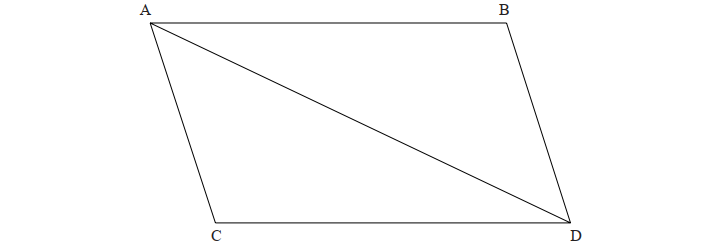
\includegraphics[width=0.75\linewidth]{image/Text3/Fig3.1.png}
\end{figure}
\noindent Let a body in a given time, by force M alone impressed in A, be carried with uniform motion from A to B, and, by force N alone impressed in the same place, be carried from A to C; then complete the parallelogram ABDC, and by both forces the body will be carried in the same time along the diagonal from A to D. For, since force N acts along the line AC parallel to BD, this force, by law 2, will make no change at all in the velocity toward the line BD which is generated by the other force. Therefore, the body will reach the line BD in the same time whether force N is impressed or not, and so at the end of that time will be found somewhere on the line BD. By the same argument, at the end of the same time it will be found somewhere on the line CD, and accordingly it is necessarily found at the intersection D of both lines. And, by law 1, it will go with [uniform] rectilinear motion from A to D.\\
设一个物体在给定时间内,仅在 A 点受到力 M 的作用,以匀速从 A 运动到 B ;并且在同一位置仅受到力 N 的作用,从 A 运动到 C ;然后完成平行四边形 ABDC ,那么在这两个力的共同作用下,物体将在相同时间内沿对角线从 A 运动到 D 。因为力 N 沿着与 BD 平行的直线 AC 起作用,根据第二定律,这个力对由另一个力产生的朝向 BD 线的速度完全不会产生任何改变。因此,无论力 N 是否作用,物体都将在相同时间内到达 BD 线,所以在该时间结束时,物体将出现在 BD 线上的某个位置。通过同样的论证,在相同时间结束时,物体将出现在 CD 线上的某个位置,因此它必然出现在两条线的交点 D 处。并且,根据第一定律,它将从 A 以 [匀速] 直线运动到 D 。\\

\begin{center}
    [...]
\end{center}

\newpage
\section{Text 4 from On the Origin of Species/ \textit{Charles Darwin}}
\begin{center}
    CHAPTER IV\\
    NATURAL SELECTION
\end{center}

\addtolength{\leftskip}{1cm}
\addtolength{\rightskip}{1cm}

\noindent Natural Selection—its power compared with man's selection—its power on characters of trifling importance—its power at all ages and on both sexes—Sexual Selection—On the generality of intercrosses between individuals of the same species—Circumstances favourable and unfavourable to Natural Selection, namely, intercrossing, isolation, number of individuals—Slow action—Extinction caused by Natural Selection—Divergence of Character, related to the diversity of inhabitants of any small area, and to naturalisation—Action of Natural Selection, through Divergence of Character and Extinction, on the descendants from a common parent—Explains the Grouping of all organic beings.\\
第四章 自然选择——与人类选择的比较——其对不重要特征重要性的力量——在所有年龄和两性中的力量——性选择——同一物种个体间杂交的普遍性——有利于和不利于自然选择的情况,即杂交、隔离、个体数量——缓慢作用——自然选择导致的灭绝——特征的多样性,与任何小区域的居民多样性和自然化有关——自然选择的作用,通过特征的多样性和灭绝,对共同祖先的后代——解释所有生物的分类。\\

\addtolength{\leftskip}{-1cm}
\addtolength{\rightskip}{-1cm}

\noindent 1\\
How will the struggle for existence, discussed too briefly in the last chapter, act in regard to variation? Can the principle of selection, which we have seen is so potent in the hands of man, apply in nature? I think we shall see that it can act most effectually. Let it be borne in mind in what an endless number of strange peculiarities our domestic productions, and, in a lesser degree, those under nature, vary; and how strong the hereditary tendency is. Under domestication, it may be truly said that the whole organisation becomes in some degree plastic. Let it be borne in mind how infinitely complex and close-fitting are the mutual relations of all organic beings to each other and to their physical conditions of life. Can it, then, be thought improbable, seeing that variations useful to man have undoubtedly occurred, that other variations useful in some way to each being in the great and complex battle of life, should sometimes occur in the course of thousands of generations? If such do occur, can we doubt (remembering that many more individuals are born than can possibly survive) that individuals having any advantage, however slight, over others, would have the best chance of surviving and of procreating their kind? On the other hand, we may feel sure that any variation in the least degree injurious would be rigidly destroyed. This preservation of favourable variations and the rejection of injurious variations, I call Natural Selection. Variations neither useful nor injurious would not be affected by natural selection, and would be left a fluctuating element, as perhaps we see in the species called polymorphic.\\
上一章中简要讨论的生存斗争,会如何对变异产生影响呢?我们已经看到在人类手中极为有效的选择原理,能否在自然界中适用呢?我想我们将会看到,它能够极其有效地发挥作用。请记住,我们的家养生物存在着无数奇特的特性,在较小程度上,自然界中的生物也是如此,而且遗传倾向是多么强大。在驯化条件下,可以说整个生物机体在某种程度上都具有可塑性。还要记住,所有有机生物彼此之间以及它们与物质生活条件之间的相互关系是何等复杂且紧密相连。既然对人类有用的变异无疑已经出现,那么在漫长而复杂的生存斗争中,对每个生物在某些方面有用的其他变异,在数千代的过程中有时也会出现,这难道是不可想象的吗?如果确实出现了这样的变异,(请记住,出生的个体数量远远超过能够存活下来的数量)我们还能怀疑,那些比其他个体具有哪怕是最微小优势的个体,会有最好的生存和繁衍后代的机会吗?另一方面,我们可以肯定,任何哪怕是最轻微有害的变异都会被无情地淘汰。这种对有利变异的保留和对有害变异的摒弃,我称之为自然选择。既非有利也非有害的变异不会受到自然选择的影响,而会成为一种波动的因素,就像我们在所谓的多态性物种中可能看到的那样。\\ 

\noindent 2\\
We shall best understand the probable course of natural selection by taking the case of a country undergoing some physical change, for instance, of climate. The proportional numbers of its inhabitants would almost immediately undergo a change, and some species might become extinct. We may conclude, from what we have seen of the intimate and complex manner in which the inhabitants of each country are bound together, that any change in the numerical proportions of some of the inhabitants, independently of the change of climate itself, would most seriously affect many of the others. If the country were open on its borders, new forms would certainly immigrate, and this also would seriously disturb the relations of some of the former inhabitants. Let it be remembered how powerful the influence of a single introduced tree or mammal has been shown to be. But in the case of an island, or of a country partly surrounded by barriers, into which new and better adapted forms could not freely enter, we should then have places in the economy of nature which would assuredly be better filled up, if some of the original inhabitants were in some manner modified; for, had the area been open to immigration, these same places would have been seized on by intruders. In such case, every slight modification, which in the course of ages chanced to arise, and which in any way favoured the individuals of any of the species, by better adapting them to their altered conditions, would tend to be preserved; and natural selection would thus have free scope for the work of improvement.\\
我们可以通过考虑一个国家经历一些物理变化,例如气候的变化,来最好地理解自然选择的可能过程。其居民的比例数量几乎会立即发生变化,一些物种可能会灭绝。我们可以从我们所看到的每个国家的居民之间紧密而复杂的联系中得出结论,即一些居民的数量比例的任何变化,无论气候本身的改变如何,都会严重影响许多其他居民。如果该国边境开放,新的物种肯定会移民进来,这也将严重扰乱一些原有居民的关系。请记住,引入单一树种或哺乳动物的影响已被证明是强大的。但在岛屿或部分被屏障包围的国家的情况下,新的和更好的适应形式不能自由进入,我们就会在自然经济中有一些地方,如果一些原有居民以某种方式被改变,这些地方肯定会被更好地填满;因为,如果该地区对移民开放,这些地方就会被入侵者占据。在这种情况下,每一个偶然出现的微小变化,如果以任何方式有利于物种中的个体,通过更好地适应他们的改变条件,就会倾向于被保留下来;因此自然选择将有充分的空间进行改进工作。

\noindent 3\\
We have reason to believe, as stated in the first chapter, that a change in the conditions of life, by specially acting on the reproductive system, causes or increases variability; and in the foregoing case the conditions of life are supposed to have undergone a change, and this would manifestly be favourable to natural selection, by giving a better chance of profitable variations occurring; and unless profitable variations do occur, natural selection can do nothing. Not that, as I believe, any extreme amount of variability is necessary; as man can certainly produce great results by adding up in any given direction mere individual differences, so could Nature, but far more easily, from having incomparably longer time at her disposal. Nor do I believe that any great physical change, as of climate, or any unusual degree of isolation to check immigration, is actually necessary to produce new and unoccupied places for natural selection to fill up by modifying and improving some of the varying inhabitants. For as all the inhabitants of each country are struggling together with nicely balanced forces, extremely slight modifications in the structure or habits of one inhabitant would often give it an advantage over others; and still further modifications of the same kind would often still further increase the advantage. No country can be named in which all the native inhabitants are now so perfectly adapted to each other and to the physical conditions under which they live, that none of them could anyhow be improved; for in all countries, the natives have been so far conquered by naturalised productions, that they have allowed foreigners to take firm possession of the land. And as foreigners have thus everywhere beaten some of the natives, we may safely conclude that the natives might have been modified with advantage, so as to have better resisted such intruders.\\
我们有理由相信,正如第一章所述,生活条件的变化,通过特别作用于生殖系统,会引起或增加变异性;在前述情况下,生活条件被认为已经发生了变化,这显然有利于自然选择,因为它提供了更好的机会让有利的变异发生;除非有利的变异确实发生,否则自然选择无能为力。我并不认为,如我相信的那样,需要任何极端的变异量;正如人类可以通过在任何给定方向上累加单纯的个体差异来产生巨大的结果,大自然也可以,但更容易,因为它拥有无比更长的时间。我也不相信任何巨大的物理变化,如气候的变化,或任何不寻常的隔离程度来阻止移民,实际上都是必需的,以产生新的和未被占据的位置,供自然选择通过修改和改进一些变化的居民来填补。因为每个国家的居民都在用平衡的力量一起奋斗,一个居民的结构或习惯的极其微小的修改往往会给它带来比其他人的优势;而且同类型的进一步修改往往会进一步增加优势。没有一个国家可以被命名,其中所有的本地居民现在都如此完美地适应彼此和他们生活的物理条件,以至于他们中的任何一个都无法以任何方式得到改善;因为在所有国家,本地居民已经被归化的物种征服到如此程度,以至于他们允许外国人牢固地占有土地。由于外国人在各地都击败了一些本地居民,我们可以安全地得出结论,本地居民可能已经被有利地修改,以便更好地抵抗这些入侵者。

\noindent 4\\
As man can produce and certainly has produced a great result by his methodical and unconscious means of selection, what may not nature effect? Man can act only on external and visible characters: nature cares nothing for appearances, except in so far as they may be useful to any being. She can act on every internal organ, on every shade of constitutional difference, on the whole machinery of life. Man selects only for his own good; Nature only for that of the being which she tends. Every selected character is fully exercised by her; and the being is placed under well-suited conditions of life. Man keeps the natives of many climates in the same country; he seldom exercises each selected character in some peculiar and fitting manner; he feeds a long and a short beaked pigeon on the same food; he does not exercise a long-backed or long-legged quadruped in any peculiar manner; he exposes sheep with long and short wool to the same climate. He does not allow the most vigorous males to struggle for the females. He does not rigidly destroy all inferior animals, but protects during each varying season, as far as lies in his power, all his productions. He often begins his selection by some half-monstrous form; or at least by some modification prominent enough to catch his eye, or to be plainly useful to him. Under nature, the slightest difference of structure or constitution may well turn the nicely-balanced scale in the struggle for life, and so be preserved. How fleeting are the wishes and efforts of man! how short his time! and consequently how poor will his products be, compared with those accumulated by nature during whole geological periods. Can we wonder, then, that nature's productions should be far "truer" in character than man's productions; that they should be infinitely better adapted to the most complex conditions of life, and should plainly bear the stamp of far higher workmanship?\\
由于人类能够通过他有条理的无意识选择手段产生并确实产生了巨大的成果,大自然又会产生什么效果呢?人类只能作用于外部和可见的特征:大自然对外表毫不在意,除非它们对任何生物可能有用。她可以作用于每一个内部器官,每一种体质差异,整个生命机制。人类仅为自己的利益选择;大自然只为她所倾向的生物选择。每一个被选择的特征都被她充分运用;并且生物被置于适合的生活条件下。人类将许多气候的土著保持在同一个国家;他很少以某种特殊和合适的方式运用每一个被选择的特征;他用同样的食物喂养长喙和短喙的鸽子;他不会以任何特殊方式锻炼长背或长腿的四足动物;他将长毛和短毛的羊暴露在相同的气候下。他不允许最强壮的雄性为雌性而斗争。他不会严格地消灭所有劣等动物,而是在每个不同的季节里,尽其所能保护他所有的产品。他经常以某种半畸形的形式开始他的选择;或者至少以某种足够突出的修改开始,足以吸引他的目光,或对他明显有用。在大自然中,结构或体质上的最微小差异可能会很好地改变生命斗争中微妙平衡的天平,从而得以保留。人类的愿望和努力是多么短暂!他的时间是多么短暂!因此,与大自然在整个地质时期积累的产品相比,他的产品将是多么贫乏。那么,我们能不惊奇吗,大自然的产物在性格上应该比人类的产品远为“真实”;它们应该无限地更好地适应最复杂的生活条件,并明显地带有更高工艺的标志?

\noindent 5\\
It may be said that natural selection is daily and hourly scrutinising throughout the world, every variation, even the slightest; rejecting that which is bad, preserving and adding up all that is good; silently and insensibly working, whenever and wherever opportunity offers, at the improvement of each organic being in relation to its organic and inorganic conditions of life. We see nothing of these slow changes in progress, until the hand of time has marked the long lapse of ages, and then so imperfect is our view into long past geological ages, that we only see that the forms of life are now different from what they formerly were.\\
可以说,自然选择每天都在每时每刻审视着全世界的每一个变异,甚至是最微小的变异;淘汰坏的,保留并积累所有好的;在机会出现时,无论何时何地都在默默地、不知不觉地工作,以改善每个生物体与其有机和无机的生活条件的关系。我们看不到这些缓慢变化的进展,直到时间之手标记了漫长的岁月流逝,然后我们对遥远的地质年代的看法是如此不完美,以至于我们只看到生命的形式现在已经不同于它们以前的样子。

\noindent 6\\
Although natural selection can act only through and for the good of each being, yet characters and structures, which we are apt to consider as of very trifling importance, may thus be acted on. When we see leaf-eating insects green, and bark-feeders mottled-grey; the alpine ptarmigan white in winter, the red-grouse the colour of heather, and the black-grouse that of peaty earth, we must believe that these tints are of service to these birds and insects in preserving them from danger. Grouse, if not destroyed at some period of their lives, would increase in countless numbers; they are known to suffer largely from birds of prey; and hawks are guided by eyesight to their prey,—so much so, that on parts of the Continent persons are warned not to keep white pigeons, as being the most liable to destruction. Hence I can see no reason to doubt that natural selection might be most effective in giving the proper colour to each kind of grouse, and in keeping that colour, when once acquired, true and constant. Nor ought we to think that the occasional destruction of an animal of any particular colour would produce little effect: we should remember how essential it is in a flock of white sheep to destroy every lamb with the faintest trace of black. In plants the down on the fruit and the colour of the flesh are considered by botanists as characters of the most trifling importance: yet we hear from an excellent horticulturist, Downing, that in the United States smooth-skinned fruits suffer far more from a beetle, a curculio, than those with down; that purple plums suffer far more from a certain disease than yellow plums; whereas another disease attacks yellow-fleshed peaches far more than those with other coloured flesh. If, with all the aids of art, these slight differences make a great difference in cultivating the several varieties, assuredly, in a state of nature, where the trees would have to struggle with other trees and with a host of enemies, such differences would effectually settle which variety, whether a smooth or downy, a yellow or purple fleshed fruit, should succeed.\\
尽管自然选择只能通过并为了每个生物的利益而起作用,但我们倾向于认为非常微不足道的特征和结构,可能因此受到作用。当我们看到食叶昆虫是绿色的,食树皮的昆虫是斑驳的灰色;冬季的高山雷鸟是白色的,红松鸡是石楠的颜色,黑松鸡是泥炭土的颜色,我们必须相信这些颜色对这些鸟类和昆虫在保护它们免受危险方面是有帮助的。松鸡如果在它们生命中的某个时期没有被消灭,它们的数量会无限增加;它们被猛禽大量捕食;鹰是通过视力来寻找猎物的,这种视力非常敏锐,以至于在欧洲大陆的某些地方,人们被警告不要饲养白色的鸽子,因为它们最容易被捕食。因此,我看不出有任何理由怀疑自然选择可能在赋予每种松鸡适当的颜色方面最为有效,并在获得这种颜色后,保持这种颜色的真实和恒定。我们也不应该认为偶尔消灭某种特定颜色的动物会产生很小的影响:我们应该记住,在一群白色的羊中,消灭每一只带有最微弱黑色痕迹的羊羔是多么重要。在植物中,果实上的绒毛和果肉的颜色被植物学家认为是微不足道的特征:然而,我们从一位优秀的园艺学家唐宁那里听说,在美国,光滑皮肤的果实比有绒毛的果实更容易受到一种叫做象鼻虫的甲虫的侵害;紫色的李子比黄色的李子更容易受到某种疾病的侵害;而另一种疾病则对黄色果肉的桃子的侵害远大于其他颜色的果肉。如果,在所有艺术的帮助下,这些微小的差异在培育几个品种时产生了很大的差异,那么,在自然状态下,树木必须与其他树木和许多敌人作斗争,这些差异将有效地决定哪种品种,无论是光滑还是有绒毛的,黄色或紫色果肉的果实,应该成功。

\noindent 9\\
Natural selection will modify the structure of the young in relation to the parent, and of the parent in relation to the young. In social animals it will adapt the structure of each individual for the benefit of the community; if each in consequence profits by the selected change. What natural selection cannot do, is to modify the structure of one species, without giving it any advantage, for the good of another species; and though statements to this effect may be found in works of natural history, I cannot find one case which will bear investigation. A structure used only once in an animal’s whole life, if of high importance to it, might be modified to any extent by natural selection; for instance, the great jaws possessed by certain insects, and used exclusively for opening the cocoon—or the hard tip to the beak of nestling birds, used for breaking the egg. It has been asserted, that of the best short-beaked tumbler-pigeons more perish in the egg than are able to get out of it; so that fanciers assist in the act of hatching. Now, if nature had to make the beak of a full-grown pigeon very short for the bird’s own advantage, the process of modification would be very slow, and there would be simultaneously the most rigorous selection of the young birds within the egg, which had the most powerful and hardest beaks, for all with weak beaks would inevitably perish: or, more delicate and more easily broken shells might be selected, the thickness of the shell being known to vary like every other structure.\\
自然选择将根据亲代调整幼体的结构,以及根据幼体调整亲代的结构。在群居动物中,它将为群体的利益调整每个个体的结构;如果每个个体因此从所选择的变化中获益。自然选择不能做的是,在不给某一物种任何优势的情况下,为了另一物种的利益而改变其结构;尽管在自然历史作品中可以找到这种效果的陈述,但我找不到一个经得起调查的案例。一个动物一生中只使用一次的结构,如果对它非常重要,可能会被自然选择修改到任何程度;例如,某些昆虫拥有的巨大颚部,专门用于打开茧——或者雏鸟喙的硬尖,用于打破蛋壳。有人断言,最好的短喙翻飞鸽在蛋中的死亡率比能够破壳而出的要高;因此,饲养者协助孵化过程。现在,如果大自然必须为了鸟类自身的优势而使成年鸽子的喙非常短,那么修改过程将会非常缓慢,并且同时会对蛋中的幼鸟进行最严格的选择,选择那些拥有最强大和最坚硬喙的幼鸟,因为所有喙弱的都不可避免地会死亡:或者,可能会选择更精致、更容易破碎的蛋壳,因为已知蛋壳的厚度像其他任何结构一样会有所不同。

\noindent 10\\
\textit{Sexual Selection.}—inasmuch as peculiarities often appear under domestication in one sex and become hereditarily attached to that sex, the same fact probably occurs under nature, and if so, natural selection will be able to modify one sex in its functional relations to the other sex, or in relation to wholly different habits of life in the two sexes, as is sometimes the case with insects. And this leads me to say a few words on what I call \textit{Sexual Selection}. This depends, not on a struggle for existence, but on a struggle between the males for possession of the females; the result is not death to the unsuccessful competitor, but few or no offspring. Sexual selection is, therefore, less rigorous than natural selection. Generally, the most vigorous males, those which are best fitted for their places in nature, will leave most progeny. But in many cases, victory will depend not on general vigour, but on having special weapons, confined to the male sex. A hornless stag or spurless cock would have a poor chance of leaving offspring. Sexual selection by always allowing the victor to breed might surely give indomitable courage, length to the spur, and strength to the wing to strike in the spurred leg, as well as the brutal cock-fighter, who knows well that he can improve his breed by careful selection of the best cocks. How low in the scale of nature this law of battle descends, I know not; male alligators have been described as fighting, bellowing, and whirling round, like Indians in a war-dance, for the possession of the females; male salmons have been seen fighting all day long; male stag-beetles often bear wounds from the huge mandibles of other males. The war is, perhaps, severest between the males of polygamous animals, and these seem oftenest provided with special weapons. The males of carnivorous animals are already well armed; though to them and to others, special means of defence may be given through means of sexual selection, as the mane to the lion, the shoulder-pad to the boar, and the hooked jaw to the male salmon; for the shield may be as important for victory, as the sword or spear.\\
\textit{性选择}。—由于在圈养条件下,一些特征经常出现在一种性别中,并遗传性地附着于该性别,同样的事实可能在自然界中发生,如果是这样,自然选择将能够修改一个性别在与另一性别的功能关系中,或与两性完全不同的生活习性的关系中,就像有时昆虫的情况那样。这使我要说一些关于我所说的\textit{性选择}的话。这并不取决于生存斗争,而是取决于雄性之间为争夺雌性而进行的斗争;结果不是对失败者造成死亡,而是后代稀少或没有。因此,性选择比自然选择不那么严格。一般来说,最强壮的雄性,那些最适合它们在自然界中的位置的,将留下最多的后代。但在许多情况下,胜利将不取决于一般活力,而取决于拥有仅限于雄性的特殊武器。没有角的雄鹿或没有距的公鸡留下后代的机会很小。性选择总是允许胜利者繁殖,肯定可以赋予无可战胜的勇气,距的长度,以及在距腿上打击的翅膀的力量,以及残忍的斗鸡者,他很清楚他可以通过仔细选择最好的公鸡来改善他的品种。这种战斗法则在自然界的尺度上下降到多低,我不知道;有人描述雄性短吻鳄为争夺雌性而战斗、咆哮和旋转,就像印第安人的战舞;有人看到雄性鲑鱼整天战斗;雄性鹿角甲虫常常带着其他雄性巨大颚部造成的伤口。战争可能在一夫多妻制动物的雄性之间最为激烈,这些动物似乎最常配备特殊武器。食肉动物的雄性已经很好地武装起来;尽管对它们和对其他动物,可以通过性选择手段获得特殊的防御手段,如狮子的鬃毛、野猪的肩垫和雄性鲑鱼的钩状颚;因为盾牌对于胜利可能和剑或矛一样重要。

\noindent 11\\
Amongst birds, the contest is often of a more peaceful character. All those who have attended to the subject, believe that there is the severest rivalry between the males of many species to attract by singing the females. The rock-thrush of Guiana, birds of Paradise, and some others, congregate; and successive males display their gorgeous plumage and perform strange antics before the females, which standing by as spectators, at last choose the most attractive partner. Those who have closely attended to birds in confinement well know that they often take individual preferences and dislikes: thus Sir R. Heron has described how one pied peacock was eminently attractive to all his hen birds. It may appear childish to attribute any effect to such apparently weak means: I cannot here enter on the details necessary to support this view; but if man can in a short time give elegant carriage and beauty to his bantams, according to his standard of beauty, I can see no good reason to doubt that female birds, by selecting, during thousands of generations, the most melodious or beautiful males, according to their standard of beauty, might produce a marked effect. I strongly suspect that some well-known laws with respect to the plumage of male and female birds, in comparison with the plumage of the young, can be explained on the view of plumage having been chiefly modified by sexual selection, acting when the birds have come to the breeding age or during the breeding season; the modifications thus produced being inherited at corresponding ages or seasons, either by the males alone, or by the males and females; but I have not space here to enter on this subject.\\
在鸟类中,竞争往往具有更和平的性质。所有关注这一主题的人都相信,许多物种的雄性之间存在着最激烈的竞争,以歌声吸引雌性。圭亚那的岩鸫、天堂鸟和其他一些鸟类会聚集在一起;连续的雄性在雌性面前展示它们华丽的羽毛并表演奇怪的动作,雌性则作为旁观者站在一旁,最终选择最具吸引力的伴侣。那些在圈养中仔细观察过鸟类的人很清楚,它们经常会有个人的喜好和厌恶:例如,R·赫伦爵士描述了一只杂色孔雀对他的所有雌鸟都非常有吸引力。将任何效果归因于这种表面上的微弱手段可能看起来有些幼稚:我不能在这里详细阐述支持这一观点的必要细节;但如果人类能在短时间内根据自己对美的标准赋予他的观赏鸡以优雅的举止和美丽,我看不出有任何充分的理由怀疑,雌性鸟类通过在数千代中选择最悦耳或最美丽的雄性,根据它们对美的标准,可能会产生显著的效果。我强烈怀疑,一些关于雄性和雌性鸟类羽毛与幼鸟羽毛相比的众所周知的规律,可以根据羽毛主要通过性选择进行修改的观点来解释,这种修改发生在鸟类达到繁殖年龄或繁殖季节时;由此产生的这些修改在相应的年龄或季节中被继承,无论是仅由雄性还是由雄性和雌性;但是我在这里没有空间进一步讨论这个问题。\\

\noindent 12\\
Thus it is, as I believe, that when the males and females of any animal have the same general habits of life, but differ in structure, colour, or ornament, such differences have been mainly caused by sexual selection; that is, individual males have had, in successive generations, some slight advantage over other males, in their weapons, means of defence, or charms; and have transmitted these advantages to their male offspring. Yet, I would not wish to attribute all such sexual differences to this agency: for we see peculiarities arising and becoming attached to the male sex in our domestic animals (as the wattle in male carriers, horn-like protuberances in the cocks of certain fowls, \&c.), which we cannot believe to be either useful to the males in battle, or attractive to the females. We see analogous cases under nature, for instance, the tuft of hair on the breast of the turkey-cock, which can hardly be either useful or ornamental to this bird; indeed, had the tuft appeared under domestication, it would have been called a monstrosity.//
因此,我相信,当任何动物的雄性和雌性具有相同的一般生活习惯,但在结构、颜色或装饰上有所不同时,这些差异主要是由性选择引起的;也就是说,个别雄性在连续的世代中,相对于其他雄性在武器、防御手段或魅力方面拥有一些微小的优势;并将这些优势传递给它们的雄性后代。然而,我不希望将所有这些性别差异都归因于这种机制:因为我们在我们驯养的动物中看到一些特征出现并附着于雄性(如雄性家禽的垂肉、某些家禽公鸡的角状突起等),我们不相信这些特征对雄性在战斗中有用,或对雌性有吸引力。我们在自然界中看到类似的情况,例如,火鸡公鸡胸前的一簇毛发,这对这种鸟来说几乎不可能有用或装饰性;实际上,如果这簇毛发是在驯化下出现的,它将被称为怪物。

\noindent 13\\
Illustrations of the action of Natural Selection.—in order to make it clear how, as I believe, natural selection acts, I must beg permission to give one or two imaginary illustrations. Let us take the case of a wolf, which preys on various animals, securing some by craft, some by strength, and some by fleetness; and let us suppose that the fleetest prey, a deer for instance, had from any change in the country increased in numbers, or that other prey had decreased in numbers, during that season of the year when the wolf is hardest pressed for food. I can under such circumstances see no reason to doubt that the swiftest and slimmest wolves would have the best chance of surviving, and so be preserved or selected,—provided always that they retained strength to master their prey at this or at some other period of the year, when they might be compelled to prey on other animals. I can see no more reason to doubt this, than that man can improve the fleetness of his greyhounds by careful and methodical selection, or by that unconscious selection which results from each man trying to keep the best dogs without any thought of modifying the breed. wolves would have the best chance of surviving, and so be preserved or selected, provided always that they retained strength to master their prey at this or at some other period of the year, when they might be compelled to prey on other animals. I can see no more reason to doubt this, than that man can improve the fleetness of his greyhounds by careful and methodical selection, or by that unconscious selection which results from each man trying to keep the best dogs without any thought of modifying the breed.\\
自然选择作用的例证。为了清楚地说明,如我相信的那样,自然选择是如何作用的,我必须请求允许给出一到两个假想的例证。让我们以狼为例,它捕食各种动物,有些通过狡诈,有些通过力量,有些通过敏捷;假设最敏捷的猎物,例如鹿,由于国家的任何变化而数量增加,或者在狼最需要食物的那一年的其他猎物数量减少。在这种情况下,我看不出有任何理由怀疑最迅速和最苗条的狼将有最大的生存机会,因此被保存或选择,前提是它们始终保持力量,在这一年的这个时候或在其他某个时期,当它们可能被迫捕食其他动物时,掌握它们的猎物。我看不出对此有任何怀疑的理由,就像人类可以通过仔细和有条理的选择,或者通过每个人试图保留最好的狗而不去考虑改变品种的无意识选择来提高灵缇的敏捷性一样。狼将有最大的生存机会,因此被保存或选择,前提是它们始终保持力量,在这一年的这个时候或在其他某个时期,当它们可能被迫捕食其他动物时,掌握它们的猎物。我看不出对此有任何怀疑的理由,就像人类可以通过仔细和有条理的选择,或者通过每个人试图保留最好的狗而不去考虑改变品种的无意识选择来提高灵缇的敏捷性一样。\textbf{有问题}

\noindent 14\\


\noindent 15\\
Let us now take a more complex case. Certain plants excrete a sweet juice, apparently for the sake of eliminating something injurious from their sap: this is effected by glands at the base of the stipules in some Leguminosae, and at the back of the leaf of the common laurel. This juice, though small in quantity, is greedily sought by insects. Let us now suppose a little sweet juice or nectar to be excreted by the inner bases of the petals of a flower. In this case insects in seeking the nectar would get dusted with pollen, and would certainly often transport the pollen from one flower to the stigma of another flower. The flowers of two distinct individuals of the same species would thus get crossed; and the act of crossing, we have good reason to believe (as will hereafter be more fully alluded to), would produce very vigorous seedlings, which consequently would have the best chance of flourishing and surviving. Some of these seedlings would probably inherit the nectar-excreting power. Those individual flowers which had the largest glands or nectaries, and which excreted most nectar, would be oftenest visited by insects, and would be oftenest crossed; and so in the long-run would gain the upper hand. Those flowers, also, which had their stamens and pistils placed, in relation to the size and habits of the particular insects which visited them, so as to favour in any degree the transportal of their pollen from flower to flower, would likewise be favoured or selected. We might have taken the case of insects visiting flowers for the sake of collecting pollen instead of nectar; and as pollen is formed for the sole object of fertilisation, its destruction appears a simple loss to the plant; yet if a little pollen were carried, at first occasionally and then habitually, by the pollen-devouring insects from flower to flower, and a cross thus effected, although nine-tenths of the pollen were destroyed, it might still be a great gain to the plant; and those individuals which produced more and more pollen, and had larger and larger anthers, would be selected.\\
现在让我们来看一个更复杂的例子。某些植物会分泌一种甜汁,显然是为了从树液中排出某些有害物质:在一些豆科植物中,这是由托叶基部的腺体来完成的,而在月桂树中则是由叶子背面的腺体来完成。这种甜汁虽然量少,但却受到昆虫的极力寻觅。现在让我们假设一朵花的花瓣内侧基部会分泌少量甜汁或花蜜。在这种情况下,昆虫在寻觅花蜜时身上会沾上花粉,并且肯定会经常把花粉从一朵花带到另一朵花的柱头上。这样,同一物种的两株不同植株的花就会进行杂交;我们有充分的理由相信(后面会更全面地提及这一点),杂交行为会产生非常茁壮的幼苗,因此这些幼苗有最好的机会茁壮成长并存活下来。其中一些幼苗可能会遗传分泌花蜜的能力。那些拥有最大的腺体或蜜腺且分泌最多花蜜的花朵,会最常被昆虫光顾,也会最常进行杂交;从长远来看,它们会占据优势。此外,那些其雄蕊和雌蕊的着生位置,相对于光顾它们的特定昆虫的体型和习性,在任何程度上都有利于花粉在花朵间传播的花朵,同样也会受到青睐或被选择。我们本可以举昆虫为采集花粉而非花蜜而光顾花朵的例子;由于花粉的形成唯一目的是为了受精,所以花粉的损耗对植物来说似乎是一种纯粹的损失;然而,如果有少量花粉,一开始是偶尔地,后来则是习惯性地,被以花粉为食的昆虫从一朵花带到另一朵花,从而实现杂交,尽管十分之九的花粉被损耗了,但对植物来说可能仍然是一个巨大的收益;而那些产生越来越多花粉且花药越来越大的植株个体就会被选择出来。 

\noindent 16\\
When our plant, by this process of the continued preservation or natural selection of more and more attractive flowers, had been rendered highly attractive to insects, they would, unintentionally on their part, regularly carry pollen from flower to flower; and that they can most effectually do this, I could easily show by many striking instances. I will give only one—not as a very striking case, but as likewise illustrating one step in the separation of the sexes of plants, presently to be alluded to. Some holly-trees bear only male flowers, which have four stamens producing rather a small quantity of pollen, and a rudimentary pistil; other holly-trees bear only female flowers; these have a full-sized pistil, and four stamens with shrivelled anthers, in which not a grain of pollen can be detected. Having found a female tree exactly sixty yards from a male tree, I put the stigmas of twenty flowers, taken from different branches, under the microscope, and on all, without exception, there were pollen-grains, and on some a profusion of pollen. As the wind had set for several days from the female to the male tree, the pollen could not thus have been carried. The weather had been cold and boisterous, and therefore not favourable to bees, nevertheless every female flower which I examined had been effectually fertilised by the bees, accidentally dusted with pollen, having flown from tree to tree in search of nectar. But to return to our imaginary case: as soon as the plant had been rendered so highly attractive to insects that pollen was regularly carried from flower to flower, another process might commence. No naturalist doubts the advantage of what has been called the “physiological division of labour;” hence we may believe that it would be advantageous to a plant to produce stamens alone in one flower or on one whole plant, and pistils alone in another flower or on another plant. In plants under culture and placed under new conditions of life, sometimes the male organs and sometimes the female organs become more or less impotent; now if we suppose this to occur in ever so slight a degree under nature, then as pollen is already carried regularly from flower to flower, and as a more complete separation of the sexes of our plant would be advantageous on the principle of the division of labour, individuals with this tendency more and more increased, would be continually favoured or selected, until at last a complete separation of the sexes would be effected.\\
当我们所讨论的植物,通过对越来越具吸引力的花朵持续留存或自然选择的过程,变得对昆虫极具吸引力时,昆虫就会在无意中频繁地将花粉从一朵花带到另一朵花。而且,它们能够高效地做到这一点,我可以通过许多显著的例子轻易证明。我仅举一个例子——这个例子并非特别典型,但同样可以说明植物性别分离过程中的一个步骤,稍后会提及这一点。一些冬青树只开雄花,雄花有四枚雄蕊,产生的花粉量较少,还有一个退化的雌蕊;另一些冬青树只开雌花,雌花有发育完全的雌蕊,以及四枚花药萎缩的雄蕊,在这些萎缩的花药中检测不到一粒花粉。我发现一棵雌树与一棵雄树相距恰好六十码,我将从不同树枝上取下的二十朵雌花的柱头放在显微镜下观察,无一例外,柱头上都有花粉粒,有些柱头上甚至布满了花粉。由于连续几天风向都是从雌树吹向雄树,所以花粉不可能是被风吹来的。当时天气寒冷且狂风大作,因此不利于蜜蜂活动,然而我检查过的每一朵雌花却都被蜜蜂成功授粉了,这些蜜蜂在从一棵树飞到另一棵树寻觅花蜜时,身上意外地沾上了花粉。现在回到我们设想的情况:一旦植物对昆虫极具吸引力,使得花粉能有规律地在花朵间传播,另一个过程就可能开始了。没有博物学家会怀疑所谓 “生理分工” 的优势;因此我们可以相信,对一株植物来说,在一朵花或一整株植物上只产生雄蕊,而在另一朵花或另一株植物上只产生雌蕊,是有好处的。在人工培育且处于新环境下的植物中,有时雄性器官,有时雌性器官会或多或少地失去功能;现在如果我们设想在自然环境中也会发生哪怕极其轻微的这种情况,那么由于花粉已经有规律地在花朵间传播,而且根据分工原则,植物性别更完全的分离是有利的,那么具有这种倾向且越来越明显的个体就会不断受到青睐或被选择,直到最终实现植物性别的完全分离。 

\noindent 17\\
Let us now turn to the nectar-feeding insects in our imaginary case: we may suppose the plant of which we have been slowly increasing the nectar by continued selection, to be a common plant; and that certain insects depended in main part on its nectar for food. I could give many facts, showing how anxious bees are to save time; for instance, their habit of cutting holes and sucking the nectar at the bases of certain flowers, which they can, with a very little more trouble, enter by the mouth. Bearing such facts in mind, I can see no reason to doubt that an accidental deviation in the size and form of the body, or in the curvature and length of the proboscis, \&c., far too slight to be appreciated by us, might profit a bee or other insect, so that an individual so characterised would be able to obtain its food more quickly, and so have a better chance of living and leaving descendants. Its descendants would probably inherit a tendency to a similar slight deviation of structure. The tubes of the corollas of the common red and incarnate clovers (Trifolium pratense and incarnatum) do not on a hasty glance appear to differ in length; yet the hive-bee can easily suck the nectar out of the incarnate clover, but not out of the common red clover, which is visited by humble-bees alone; so that whole fields of the red clover offer in vain an abundant supply of precious nectar to the hive-bee. Thus it might be a great advantage to the hive-bee to have a slightly longer or differently constructed proboscis. On the other hand, I have found by experiment that the fertility of clover greatly depends on bees visiting and moving parts of the corolla, so as to push the pollen on to the stigmatic surface. Hence, again, if humble-bees were to become rare in any country, it might be a great advantage to the red clover to have a shorter or more deeply divided tube to its corolla, so that the hive-bee could visit its flowers. Thus I can understand how a flower and a bee might slowly become, either simultaneously or one after the other, modified and adapted to each other, by the continued preservation of individuals presenting mutual and slightly favourable deviations of structure.\\
现在让我们回到我们设想例子中的吸食花蜜的昆虫:我们可以假定,通过持续选择而使花蜜量慢慢增加的植物是一种常见植物,并且某些昆虫主要以其花蜜为食。我可以列举许多事实,来说明蜜蜂是多么急于节省时间;例如,它们有在某些花朵基部打孔并吸食花蜜的习性,而其实它们只需多费一点劲,就可以从花朵的开口处进入。考虑到这些事实,我毫不怀疑,蜜蜂身体大小和形状,或者口器的弯曲度和长度等方面的一些细微变化,细微到我们难以察觉,但可能会对蜜蜂或其他昆虫有益,这样具有这些特征的个体就能更快地获取食物,从而有更好的生存和繁衍后代的机会。其后代可能会遗传这种结构上的轻微变异倾向。普通红三叶草和绛三叶草(车轴草属的红车轴草和绛车轴草)花冠的花管,乍一看长度似乎没有区别;然而,蜜蜂能轻易地从绛三叶草中吸食花蜜,却无法从普通红三叶草中吸食,因为只有熊蜂会光顾普通红三叶草;所以大片的红三叶草田为蜜蜂提供了丰富的珍贵花蜜,但蜜蜂却无法享用。因此,对蜜蜂来说,拥有稍长一点或结构不同的口器可能会有很大的优势。另一方面,我通过实验发现,三叶草的受精情况在很大程度上取决于蜜蜂对花冠的光顾和触动,以便将花粉推到柱头表面。因此,如果在任何一个地方熊蜂变得稀少,那么对红三叶草来说,拥有更短或更深裂的花冠花管可能会有很大的优势,这样蜜蜂就能光顾它的花朵。由此我能理解,花朵和蜜蜂是如何通过持续留存那些在结构上呈现出相互且略微有利变异的个体,慢慢地同时或先后发生改变并相互适应的。\\

\noindent 18\\
I am well aware that this doctrine of natural selection, exemplified in the above imaginary instances, is open to the same objections which were at first urged against Sir Charles Lyell’s noble views on “the modern changes of the earth, as illustrative of geology;” but we now very seldom hear the action, for instance, of the coast-waves, called a trifling and insignificant cause, when applied to the excavation of gigantic valleys or to the formation of the longest lines of inland cliffs. Natural selection can act only by the preservation and accumulation of infinitesimally small inherited modifications, each profitable to the preserved being; and as modern geology has almost banished such views as the excavation of a great valley by a single diluvial wave, so will natural selection, if it be a true principle, banish the belief of the continued creation of new organic beings, or of any great and sudden modification in their structure.\\
我深知,上述假想例子中所阐述的自然选择学说,会面临与最初针对查尔斯·莱尔爵士关于 “作为地质学例证的地球近代变迁” 的卓越观点所提出的相同反对意见;但是,如今我们很少听到有人称海岸波浪的作用(例如),在涉及巨大山谷的形成或漫长内陆悬崖的塑造时,是微不足道、不值一提的原因。自然选择只能通过留存和积累极其微小的、可遗传的、对留存生物有益的变异来发挥作用;正如现代地质学几乎摒弃了诸如一次大洪水波浪就能形成一个大峡谷这样的观点一样,倘若自然选择是一条正确的原理,它也将摒弃关于新生物持续被创造出来, 或者生物结构会发生任何巨大而突然的变异这样的观念。 \\

\noindent 39\\
Extinction.—This subject will be more fully discussed in our chapter on Geology; but it must be here alluded to from being intimately connected with natural selection. Natural selection acts solely through the preservation of variations in some way advantageous, which consequently endure. But as from the high geometrical powers of increase of all organic beings, each area is already fully stocked with inhabitants, it follows that as each selected and favoured form increases in number, so will the less favoured forms decrease and become rare. Rarity, as geology tells us, is the precursor to extinction. We can, also, see that any form represented by few individuals will, during fluctuations in the seasons or in the number of its enemies, run a good chance of utter extinction. But we may go further than this; for as new forms are continually and slowly being produced, unless we believe that the number of specific forms goes on perpetually and almost indefinitely increasing, numbers inevitably must become extinct. That the number of specific forms has not indefinitely increased, geology shows us plainly; and indeed we can see reason why they should not have thus increased, for the number of places in the polity of nature is not indefinitely great,—not that we have any means of knowing that any one region has as yet got its maximum of species. Probably no region is as yet fully stocked, for at the Cape of Good Hope, where more species of plants are crowded together than in any other quarter of the world, some foreign plants have become naturalised, without causing, as far as we know, the extinction of any natives.\\
灭绝 —— 这个主题将在我们关于地质学的章节中更全面地讨论;但由于它与自然选择密切相关,所以在这里必须提及。自然选择仅仅通过留存某种有利的变异来发挥作用,这些变异因此得以持续存在。但是,由于所有生物都具有强大的几何级数增长能力,每个地区早已挤满了生物,因此,随着每一个被选择和青睐的物种数量增加,那些较不受青睐的物种数量就会减少并变得稀少。正如地质学告诉我们的,稀少是灭绝的先兆。我们还可以看到,任何个体数量稀少的物种,在季节波动或其天敌数量变化时,极有可能彻底灭绝。但我们还可以更进一步思考;由于新物种在持续且缓慢地产生,除非我们相信物种的数量会持续且几乎无限地增加,否则必然会有一些物种灭绝。地质学清楚地表明,物种的数量并没有无限增加;实际上,我们也能明白它们为何没有无限增加,因为自然界生态系统中的生态位数量并非无限多 —— 并不是说我们有办法知道任何一个地区是否已经达到了物种数量的最大值。可能没有任何一个\\

\noindent 40\\
Furthermore, the species which are most numerous in individuals will have the best chance of producing within any given period favourable variations. We have evidence of this, in the facts given in the second chapter, showing that it is the common species which afford the greatest number of recorded varieties, or incipient species. Hence, rare species will be less quickly modified or improved within any given period, and they will consequently be beaten in the race for life by the modified descendants of the commoner species.\\
此外,个体数量最多的物种在任何特定时期内产生有利变异的可能性最大。我们在第二章给出的事实中可以找到这方面的证据,这些事实表明,正是常见物种产生了数量最多的有记录的变种或初始物种。因此,稀有物种在任何特定时期内发生变异或进化的速度较慢,因此在生存竞争中,它们会被常见物种经过变异的后代所击败。 \\

\noindent 41\\
From these several considerations I think it inevitably follows, that as new species in the course of time are formed through natural selection, others will become rarer and rarer, and finally extinct. The forms which stand in closest competition with those undergoing modification and improvement, will naturally suffer most. And we have seen in the chapter on the Struggle for Existence that it is the most closely-allied forms,—varieties of the same species, and species of the same genus or of related genera,—which, from having nearly the same structure, constitution, and habits, generally come into the severest competition with each other. Consequently, each new variety or species, during the progress of its formation, will generally press hardest on its nearest kindred, and tend to exterminate them. We see the same process of extermination amongst our domesticated productions, through the selection of improved forms by man. Many curious instances could be given showing how quickly new breeds of cattle, sheep, and other animals, and varieties of flowers, take the place of older and inferior kinds. In Yorkshire, it is historically known that the ancient black cattle were displaced by the long-horns, and that these “were swept away by the short-horns” (I quote the words of an agricultural writer) “as if by some murderous pestilence.”\\
基于上述几点考虑,我认为必然会得出这样的结论:随着时间推移,新物种通过自然选择不断形成,其他物种则会变得越来越稀少,最终走向灭绝。与那些正在经历变异和进化的物种竞争最为激烈的生物类型,自然会受到最大的冲击。我们在关于 “生存斗争” 的章节中已经了解到,亲缘关系最为密切的生物类型 —— 同一物种的变种,以及同一属或相关属的物种,由于它们的结构、体质和习性几乎相同,通常会彼此展开最为激烈的竞争。因此,每一个新变种或新物种在形成过程中,通常会对与其亲缘关系最近的物种构成最大的压力,并趋于将它们灭绝。我们在人工培育的产物中也能看到同样的灭绝过程,人类会选择改良的品种。可以列举出许多有趣的例子,表明牛、羊及其他动物的新品种,以及花卉的变种,能够多么迅速地取代旧有的、品质较差的种类。在约克郡,从历史记载可知,古代的黑牛被长角牛所取代,而长角牛 “又被短角牛淘汰”(我引用一位农业作家的话),“就好像遭受了某种致命的瘟疫一样” 。 \\

\noindent 42\\
Divergence of Character.—The principle, which I have designated by this term, is of high importance on my theory, and explains, as I believe, several important facts. In the first place, varieties, even strongly-marked ones, though having somewhat of the character of species—as is shown by the hopeless doubts in many cases how to rank them—yet certainly differ from each other far less than do good and distinct species. Nevertheless, according to my view, varieties are species in the process of formation, or are, as I have called them, incipient species. How, then, does the lesser difference between varieties become augmented into the greater difference between species? That this does habitually happen, we must infer from most of the innumerable species throughout nature presenting well-marked differences; whereas varieties, the supposed prototypes and parents of future well-marked species, present slight and ill-defined differences. Mere chance, as we may call it, might cause one variety to differ in some character from its parents, and the offspring of this variety again to differ from its parent in the very same character and in a greater degree; but this alone would never account for so habitual and large an amount of difference as that between varieties of the same species and species of the same genus.\\
性状分异 —— 我用这个术语所指的原理,在我的理论中极为重要,而且我相信,它可以解释几个重要的事实。首先,变种,即使是特征明显的变种,尽管在某种程度上具有物种的特征(这从在许多情况下难以确定如何对它们进行分类就可以看出),但它们彼此之间的差异肯定远小于明确的不同物种之间的差异。然而,在我看来,变种是正在形成过程中的物种,或者如我所称的,是初始物种。那么,变种之间较小的差异是如何扩大为物种之间较大的差异的呢?我们必然会从自然界中无数呈现出明显差异的物种推断出,这种情况是经常发生的;而变种,作为未来特征明显的物种的假定原型和亲本,只呈现出细微且不明确的差异。我们所谓的纯粹偶然因素,可能会使一个变种在某些特征上与其亲本不同,而这个变种的后代又会在同一特征上与亲本有更大程度的差异;但仅凭这一点,永远无法解释同一物种的变种之间以及同一属的物种之间如此常见且巨大的差异。 

\noindent 43\\
As has always been my practice, let us seek light on this head from our domestic productions. We shall here find something analogous. A fancier is struck by a pigeon having a slightly shorter beak; another fancier is struck by a pigeon having a rather longer beak; and on the acknowledged principle that “fanciers do not and will not admire a medium standard, but like extremes,” they both go on (as has actually occurred with tumbler-pigeons) choosing and breeding from birds with longer and longer beaks, or with shorter and shorter beaks. Again, we may suppose that at an early period one man preferred swifter horses; another stronger and more bulky horses. The early differences would be very slight; in the course of time, from the continued selection of swifter horses by some breeders, and of stronger ones by others, the differences would become greater, and would be noted as forming two sub-breeds; finally, after the lapse of centuries, the sub-breeds would become converted into two well-established and distinct breeds. As the differences slowly become greater, the inferior animals with intermediate characters, being neither very swift nor very strong, will have been neglected, and will have tended to disappear. Here, then, we see in man’s productions the action of what may be called the principle of divergence, causing differences, at first barely appreciable, steadily to increase, and the breeds to diverge in character both from each other and from their common parent.\\
就像我一直以来的做法一样,让我们从家养生物中寻找关于这个问题的启示。我们会在这里发现一些类似的情况。一位养鸽爱好者注意到一只喙略短的鸽子;另一位爱好者则注意到一只喙较长的鸽子;根据 “养鸽者不欣赏也不会欣赏中等标准,而是喜欢极端特征” 这一公认原则,他们都会继续(就像在翻飞鸽中实际发生的那样)选择喙越来越长或越来越短的鸽子进行繁育。同样,我们可以设想,在早期,一个人喜欢速度更快的马,另一个人则喜欢更强壮、体型更大的马。最初的差异会非常小;随着时间的推移,一些育种者持续选择速度更快的马,而另一些人选择更强壮的马,差异就会变得更大,并逐渐形成两个亚品种;最终,几个世纪后,这些亚品种会演变成两个成熟且截然不同的品种。随着差异慢慢增大,那些具有中间特征的、既不是特别快也不是特别强壮的劣质马匹就会被忽视,并趋于消失。因此,在这里,我们在家养生物中看到了所谓 “性状分异原理” 的作用,它使起初几乎难以察觉的差异稳步增大,并且使各个品种在特征上彼此不同,也与它们的共同祖先不同 。 

\noindent 44\\
But how, it may be asked, can any analogous principle apply in nature? I believe it can and does apply most efficiently, from the simple circumstance that the more diversified the descendants from any one species become in structure, constitution, and habits, by so much will they be better enabled to seize on many and widely diversified places in the polity of nature, and so be enabled to increase in numbers.\\
但可能有人会问,类似的原理如何能在自然界中适用呢?我相信它能够而且确实能极为有效地适用,原因很简单,任何一个物种的后代在结构、体质和习性上变得越多样化,它们就越能更好地占据自然界生态系统中众多且差异极大的生态位,从而数量得以增加。 

\noindent 45\\
We can clearly see this in the case of animals with simple habits. Take the case of a carnivorous quadruped, of which the number that can be supported in any country has long ago arrived at its full average. If its natural powers of increase be allowed to act, it can succeed in increasing (the country not undergoing any change in its conditions) only by its varying descendants seizing on places at present occupied by other animals: some of them, for instance, being enabled to feed on new kinds of prey, either dead or alive; some inhabiting new stations, climbing trees, frequenting water, and some perhaps becoming less carnivorous. The more diversified in habits and structure the descendants of our carnivorous animal became, the more places they would be enabled to occupy. What applies to one animal will apply throughout all time to all animals—that is, if they vary—for otherwise natural selection can do nothing. So it will be with plants. It has been experimentally proved, that if a plot of ground be sown with one species of grass, and a similar plot be sown with several distinct genera of grasses, a greater number of plants and a greater weight of dry herbage can thus be raised. The same has been found to hold good when first one variety and then several mixed varieties of wheat have been sown on equal spaces of ground. Hence, if any one species of grass were to go on varying, and those varieties were continually selected which differed from each other in at all the same manner as distinct species and genera of grasses differ from each other, a greater number of individual plants of this species of grass, including its modified descendants, would succeed in living on the same piece of ground. And we well know that each species and each variety of grass is annually sowing almost countless seeds; and thus, as it may be said, is striving its utmost to increase its numbers. Consequently, I cannot doubt that in the course of many thousands of generations, the most distinct varieties of any one species of grass would always have the best chance of succeeding and of increasing in numbers, and thus of supplanting the less distinct varieties; and varieties, when rendered very distinct from each other, take the rank of species.\\
我们可以从习性简单的动物身上清楚地看到这一点。以一种肉食性的四足动物为例,在任何一个地区,其能够维持的数量早已达到了平均饱和水平。如果让它的自然繁殖能力发挥作用,在该地区环境条件不发生任何变化的情况下,它要增加数量,只能通过其变异的后代占据目前其他动物所占据的生态位:例如,它们中的一些能够以新的猎物为食,无论是死的还是活的;一些栖息在新的环境中,比如爬树、靠近水源,还有一些可能变得不那么肉食性。这种肉食性动物的后代在习性和结构上变得越多样化,它们能够占据的生态位就越多。适用于一种动物的情况,在任何时候对所有动物都适用 —— 也就是说,如果它们发生变异的话,否则自然选择将无法发挥作用。植物的情况也是如此。实验证明,如果在一块土地上播种一个草种,而在另一块相似的土地上播种几个不同属的草种,后者能够生长出更多的植株和更重的干草。当在同等面积的土地上先播种一个小麦变种,然后播种几个混合的小麦变种时,也发现了同样的情况。因此,如果任何一个草种持续发生变异,并且那些彼此之间的差异与不同草种和草属之间的差异相同的变种被不断选择出来,那么这个草种包括其变异后代在内的更多个体植株,就能在同一块土地上生存下来。我们都知道,每个草种和每个草的变种每年都会播撒几乎数不清的种子,可以说,它们都在竭尽全力地增加数量。因此,我毫不怀疑,在数千代的过程中,任何一个草种中差异最显著的变种总是最有机会成功生存并增加数量,从而取代差异不那么显著的变种;而当变种之间的差异变得非常明显时,它们就成为了不同的物种。 

\noindent 46\\
The truth of the principle, that the greatest amount of life can be supported by great diversification of structure, is seen under many natural circumstances. In an extremely small area, especially if freely open to immigration, and where the contest between individual and individual must be severe, we always find great diversity in its inhabitants. For instance, I found that a piece of turf, three feet by four in size, which had been exposed for many years to exactly the same conditions, supported twenty species of plants, and these belonged to eighteen genera and to eight orders, which shows how much these plants differed from each other. So it is with the plants and insects on small and uniform islets; and so in small ponds of fresh water. Farmers find that they can raise most food by a rotation of plants belonging to the most different orders: nature follows what may be called a simultaneous rotation. Most of the animals and plants which live close round any small piece of ground, could live on it (supposing it not to be in any way peculiar in its nature), and may be said to be striving to the utmost to live there; but, it is seen, that where they come into the closest competition with each other, the advantages of diversification of structure, with the accompanying differences of habit and constitution, determine that the inhabitants, which thus jostle each other most closely, shall, as a general rule, belong to what we call different genera and orders.\\
结构的高度多样化能够维持最多生命数量这一原理的正确性,在许多自然环境中都能得到体现。在一个极其狭小的区域内,尤其是在对迁入没有限制且个体之间竞争必然激烈的地方,我们总能发现生物种类的高度多样性。例如,我发现一块三英尺乘四英尺大小的草皮,多年来一直处于完全相同的环境条件下,却生长着二十种植物,这些植物分属于十八个属和八个目,这表明这些植物彼此之间差异很大。在小而单一的岛屿上的植物和昆虫,以及小型淡水池塘中的生物也是如此。农民们发现,通过轮种不同目的植物,能够收获最多的作物;大自然遵循的可以说是一种同时进行的 “轮作”。生活在任何一小块土地周围的大多数动植物,理论上都可以在这块土地上生存(假设这块土地没有特殊的性质),并且可以说都在竭尽全力地在那里生存;但是可以看到,在它们彼此竞争最为激烈的地方,结构多样化的优势,以及随之而来的习性和体质的差异,决定了那些彼此竞争最为激烈的生物,一般来说,分属于我们所说的不同的属和目。 

\noindent 50\\
After the foregoing discussion, which ought to have been much amplified, we may, I think, assume that the modified descendants of any one species will succeed by so much the better as they become more diversified in structure, and are thus enabled to encroach on places occupied by other beings. Now let us see how this principle of great benefit being derived from divergence of character, combined with the principles of natural selection and of extinction, will tend to act.\\
经过上述本应进一步展开的讨论,我认为我们可以假定,任何一个物种经过变异的后代,其结构越是多样化,就越能成功,因为这样它们就能占据其他生物所占据的生态位。现在让我们看看,从性状分异中获得巨大益处的这一原理,与自然选择和灭绝原理相结合,会如何发挥作用。 \\

\noindent 51\\
The accompanying diagram will aid us in understanding this rather perplexing subject. Let A to L represent the species of a genus large in its own country; these species are supposed to resemble each other in unequal degrees, as is so generally the case in nature, and as is represented in the diagram by the letters standing at unequal distances. I have said a large genus, because we have seen in the second chapter, that on average more of the species of large genera vary than of small genera; and the varying species of the large genera present a greater number of varieties. We have, also, seen that the species, which are the commonest and the most widely-diffused, vary more than rare species with restricted ranges. Let (A) be a common, widely-diffused, and varying species, belonging to a genus large in its own country. The little fan of diverging dotted lines of unequal lengths proceeding from (A), may represent its varying offspring. The variations are supposed to be extremely slight, but of the most diversified nature; they are not supposed all to appear simultaneously, but often after long intervals of time; nor are they all supposed to endure for equal periods. Only those variations which are in some way profitable will be preserved or naturally selected. And here the importance of the principle of benefit being derived from divergence of character comes in; for this will generally lead to the most different or divergent variations (represented by the outer dotted lines) being preserved and accumulated by natural selection. When a dotted line reaches one of the horizontal lines, and is there marked by a small numbered letter, a sufficient amount of variation is supposed to have been accumulated to have formed a fairly well-marked variety, such as would be thought worthy of record in a systematic work.\\
 随附的图表将帮助我们理解这个相当复杂的主题。设A到L代表在其所在地区属于一个大属的各个物种;这些物种彼此之间的相似程度不同,这在自然界中很常见,图表中字母之间不同的间距就体现了这一点。我提到大属,是因为我们在第二章中了解到,一般来说,大属中的物种比小属中的物种更容易发生变异;而且大属中发生变异的物种会产生更多的变种。我们还看到,那些最常见、分布最广泛的物种,比分布范围有限的稀有物种更容易发生变异。设(A)是一个常见的、分布广泛且正在变异的物种,属于其所在地区的一个大属。从(A)发出的长短不一、呈扇形散开的虚线,可以代表它变异的后代。这些变异被认为极其微小,但性质极为多样;它们并非同时出现,而是往往在很长时间间隔后才出现;而且也并非都能持续相同的时间。只有那些在某种程度上有利的变异才会被保留下来,即通过自然选择得以留存。 在这里,从性状分异中获益的原理就显得至关重要;因为这通常会导致最不同或差异最大的变异(由外侧的虚线表示)被自然选择保留并积累下来。当一条虚线到达某一条水平线,并在那里标有一个带数字的小字母时,就表示已经积累了足够多的变异,从而形成了一个特征相当明显的变种,这样的变种会被认为值得在系统的著作中记录下来。 \\

\noindent 52\\
The intervals between the horizontal lines in the diagram, may represent each a thousand generations; but it would have been better if each had represented ten thousand generations. After a thousand generations, species (A) is supposed to have produced two fairly well-marked varieties, namely $a^1$ and $m^1$. These two varieties will generally continue to be exposed to the same conditions which made their parents variable, and the tendency to variability is itself hereditary, consequently they will tend to vary, and generally to vary in nearly the same manner as their parents varied. Moreover, these two varieties, being only slightly modified forms, will tend to inherit those advantages which made their common parent (A) more numerous than most of the other inhabitants of the same country; they will likewise partake of those more general advantages which made the genus to which the parent-species belonged, a large genus in its own country. And these circumstances we know to be favourable to the production of new varieties.\\
图表中水平线之间的间隔,每个可以代表一千代;但如果每个间隔代表一万代可能会更好。经过一千代后,假定物种(A)产生了两个特征相当明显的变种,即$a^1$和$m^1$。这两个变种通常会继续处于使其亲代发生变异的相同环境条件下,而且变异的倾向本身是可遗传的,因此它们也会倾向于发生变异,并且通常会以与其亲代几乎相同的方式变异。此外,这两个变种只是稍有改变的形式,它们将倾向于继承那些使它们的共同亲代(A)在同一地区比大多数其他生物数量更多的优势;它们同样也会具备那些更普遍的优势,正是这些优势使得其亲代物种所属的属在该地区成为一个大属。我们知道,这些情况有利于新变种的产生。 \\

\noindent 53\\
If, then, these two varieties be variable, the most divergent of their variations will generally be preserved during the next thousand generations. And after this interval, variety $a^1$ is supposed in the diagram to have produced variety $a^2$, which will, owing to the principle of divergence, differ more from (A) than did variety $a^1$. Variety $m^1$ is supposed to have produced two varieties, namely $m^2$ and $s^2$, differing from each other, and more considerably from their common parent (A). We may continue the process by similar steps for any length of time; some of the varieties, after each thousand generations, producing only a single variety, but in a more and more modified condition, some producing two or three varieties, and some failing to produce any. Thus the varieties or modified descendants, proceeding from the common parent (A), will generally go on increasing in number and diverging in character. In the diagram the process is represented up to the ten - thousandth generation, and under a condensed and simplified form up to the fourteen thousandth generation.\\
那么,如果这两个变种是可变的,它们差异最大的变异通常会在接下来的一千代中被保留下来。在这段时间间隔后,图表中假定变种$a^1$产生了变种$a^2$,由于性状分异原理,$a^2$与(A)的差异会比$a^1$与(A)的差异更大。假定变种$m^1$产生了两个变种,即$m^2$和$s^2$,它们彼此不同,且与它们的共同亲代(A)的差异更大。我们可以按照类似的步骤将这个过程持续任意长的时间;有些变种在每一千代之后,只产生一个变种,但这个变种的变异程度越来越大;有些变种产生两到三个变种;还有一些变种则不产生任何后代。因此,从共同亲代(A)衍生出来的变种或经过变异的后代,其数量通常会不断增加,性状也会不断分异。在图表中,这个过程一直展示到了第一万代,并且以浓缩和简化的形式展示到了第一万四千代。 \\

\noindent 54\\
But I must here remark that I do not suppose that the process ever goes on so regularly as is represented in the diagram, though in itself made somewhat irregular. I am far from thinking that the most divergent varieties will invariably prevail and multiply: a medium form may often long endure, and may or may not produce more than one modified descendant; for natural selection will always act according to the nature of the places which are either unoccupied or not perfectly occupied by other beings; and this will depend on infinitely complex relations. But as a general rule, the more diversified in structure the descendants from any one species can be rendered, the more places they will be enabled to seize on, and the more their modified progeny will be increased. In our diagram the line of succession is broken at regular intervals by small numbered letters marking the successive forms which have become sufficiently distinct to be recorded as varieties. But these breaks are imaginary, and might have been inserted anywhere, after intervals long enough to have allowed the accumulation of a considerable amount of divergent variation.\\
但我必须在此指出,我并不认为这个过程会像图表中所展示的那样规则地进行,尽管图表本身已经表现得有些不规则了。我绝不是认为差异最大的变种总是会占优势并繁衍:中间形态往往可以长期存在,而且可能产生一个或多个变异后代,也可能不产生;因为自然选择总是根据那些尚未被其他生物占据,或者尚未被完全占据的生态位的性质来发挥作用,而这取决于极其复杂的关系。但一般来说,任何一个物种的后代在结构上越是多样化,它们能够占据的生态位就越多,其变异后代的数量也就会增加得越多。在我们的图表中,传承的线条会每隔一定间隔被带数字的小字母打断,这些字母标记着那些已经变得足够独特,可以被记录为变种的连续形态。但这些中断是假想的,只要间隔的时间足够长,足以积累大量的分异变异,它们可以被插入到任何地方。 \\

\noindent 55\\
As all the modified descendants from a common and widely - diffused species, belonging to a large genus, will tend to partake of the same advantages which made their parent successful in life, they will generally go on multiplying in number as well as diverging in character: this is represented in the diagram by the several divergent branches proceeding from (A). The modified offspring from the later and more highly improved branches in the lines of descent, will, it is probable, often take the place of, and so destroy, the earlier and less improved branches: this is represented in the diagram by some of the lower branches not reaching to the upper horizontal lines. In some cases I do not doubt that the process of modification will be confined to a single line of descent, and the number of the descendants will not be increased; although the amount of divergent modification may have been increased in the successive generations. This case would be represented in the diagram, if all the lines proceeding from (A) were removed, excepting that from $a^1$ to $a^{10}$. In the same way, for instance, the English race - horse and English pointer have apparently both gone on slowly diverging in character from their original stocks, without either having given off any fresh branches or races.\\
由于来自一个常见且分布广泛的物种(属于一个大属)的所有变异后代,往往会具备使其亲代在生存中取得成功的相同优势,所以它们通常在数量上会不断增加,同时在性状上也会不断分异:这在图表中表现为由(A)衍生出的几条分异的分支。在演化谱系中,来自较晚且改进程度更高分支的变异后代,很可能常常会取代并淘汰较早且改进程度较低的分支,图表中一些较低的分支没有延伸到上面的水平线就体现了这一点。在某些情况下,我毫不怀疑变异过程可能会局限于单一的演化谱系,后代的数量也不会增加,尽管在连续的世代中,分异变异的程度可能会增加。如果从(A)衍生出的所有分支中,只保留从$a^1$到$a^{10}$的这一支,而去掉其他分支,那么这种情况在图表中就能得以体现。例如,英国赛马和英国指示犬显然在性状上都从它们最初的种群开始慢慢发生分异,而且都没有产生新的分支或品种 。 \\

\noindent 56\\
After ten thousand generations, species (A) is supposed to have produced three forms, $a^{10}$, $f^{10}$, and $m^{10}$, which, from having diverged in character during the successive generations, will have come to differ largely, but perhaps unequally, from each other and from their common parent. If we suppose the amount of change between each horizontal line in our diagram to be excessively small, these three forms may still be only well - marked varieties; or they may have arrived at the doubtful category of sub - species; but we have only to suppose the steps in the process of modification to be more numerous or greater in amount, to convert these three forms into well - defined species: thus the diagram illustrates the steps by which the small differences distinguishing varieties are increased into the larger differences distinguishing species. By continuing the same process for a greater number of generations (as shown in the diagram in a condensed and simplified manner), we get eight species, marked by the letters between $a^{14}$ and $m^{14}$, all descended from (A). Thus, as I believe, species are multiplied and genera are formed.\\
经过一万代后,假定物种(A)产生了三个形态,即$a^{10}$、$f^{10}$和$m^{10}$,由于在连续的世代中性状发生了分异,它们彼此之间以及与它们的共同亲代之间会有很大的差异,但这种差异或许并不均等。如果我们假定图表中每条水平线之间的变化量极小,那么这三个形态可能仍然只是特征明显的变种;或者它们可能属于难以界定的亚种范畴;但我们只要设想变异过程中的步骤更多,或者变化量更大,就可以将这三个形态转变为明确的物种:因此,该图表展示了区分变种的微小差异是如何扩大为区分物种的较大差异的。通过将这个过程在更多世代中延续下去(如图表以浓缩和简化的方式所示),我们得到了八个物种,由$a^{14}$和$m^{14}$之间的字母表示,它们都源自(A)。因此,我认为,物种数量得以增加,属也得以形成。 \\

\noindent 57\\
In a large genus it is probable that more than one species would vary. In the diagram I have assumed that a second species (I) has produced, by analogous steps, after ten thousand generations, either two well-marked varieties ($w^{10}$ and $z^{10}$) or two species, according to the amount of change supposed to be represented between the horizontal lines. After fourteen thousand generations, six new species, marked by the letters $n^{14}$ to $z^{14}$, are supposed to have been produced. In each genus, the species, which are already extremely different in character, will generally tend to produce the greatest number of modified descendants; for these will have the best chance of filling new and widely different places in the polity of nature: hence in the diagram I have chosen the extreme species (A), and the nearly extreme species (I), as those which have largely varied, and have given rise to new varieties and species. The other nine species (marked by capital letters) of our original genus, may for a long period continue transmitting unaltered descendants; and this is shown in the diagram by the dotted lines not prolonged far upwards from want of space.\\
在一个大属中,很可能不止一个物种会发生变异。在图表中,我假定第二个物种(I)经过类似的步骤,在一万代之后,根据水平线之间所代表的变化量,产生了两个特征明显的变种($w^{10}$和$z^{10}$)或者两个物种。在一万四千代之后,假定产生了六个新物种,由字母$n^{14}$到$z^{10}$表示。在每个属中,那些在性状上已经极为不同的物种,通常倾向于产生数量最多的变异后代,因为这些后代最有机会占据自然界生态系统中新的、差异极大的生态位。因此在图表中,我选择了处于极端的物种(A),以及近乎极端的物种(I),作为发生了大量变异并产生新变种和新物种的代表。我们最初那个属中的其他九个物种(用大写字母表示),可能在很长一段时间内会继续繁衍出没有发生变化的后代,由于空间限制,图表中这些物种的虚线没有向上延伸很远来表示这一点。 \\

\noindent 58\\
But during the process of modification, represented in the diagram, another of our principles, namely that of extinction, will have played an important part. As in each fully stocked country natural selection necessarily acts by the selected form having some advantage in the struggle for life over other forms, there will be a constant tendency in the improved descendants of any one species to supplant and exterminate in each stage of descent their predecessors and their original parent. For it should be remembered that the competition will generally be most severe between those forms which are most nearly related to each other in habits, constitution, and structure. Hence all the intermediate forms between the earlier and later states, that is between the less and more improved state of a species, as well as the original parent - species itself, will generally tend to become extinct. So it probably will be with many whole collateral lines of descent, which will be conquered by later and improved lines of descent. If, however, the modified offspring of a species get into some distinct country, or become quickly adapted to some quite new station, in which child and parent do not come into competition, both may continue to exist.\\
但是在图表所展示的变异过程中,我们的另一个原理,即灭绝原理,也发挥了重要作用。在每一个物种饱和的地区,自然选择必然会使被选择的类型在生存竞争中比其他类型具有某种优势,因此任何一个物种的改进后代,在每一个演化阶段,都有取代并灭绝其祖先和原始亲代物种的趋势。应该记住,在习性、体质和结构上彼此最为相近的类型之间,竞争通常最为激烈。因此,一个物种早期和晚期状态之间,也就是较不改良和较改良状态之间的所有中间形态,以及原始亲代物种本身,通常都有灭绝的趋势。许多旁系的演化谱系很可能也是如此,它们会被后来出现且经过改良的演化谱系所取代。然而,如果一个物种的变异后代进入了某个不同的地区,或者迅速适应了某个全新的生态位,在那里子代和亲代不会产生竞争,那么两者可能都会继续生存下去。\\ 

\noindent 59\\
If then our diagram be assumed to represent a considerable amount of modification, species (A) and all the earlier varieties will have become extinct, having been replaced by eight new species ($a^{14}$ to $m^{14}$); and (I) will have been replaced by six ($n^{14}$ to $z^{14}$) new species.\\
那么,如果我们假定该图表代表了大量的变异,物种(A)和所有早期的变种将会灭绝,被八个新物种($a^{14}$到$m^{14}$)所取代;而物种(I)将会被六个($n^{14}$到$z^{14}$)新物种所取代 。 \\

\noindent 60\\
But we may go further than this. The original species of our genus were supposed to resemble each other in unequal degrees, as is so generally the case in nature; species (A) being more nearly related to B, C, and D, than to the other species; and species (I) more to G, H, K, L, than to the others. These two species (A) and (I), were also supposed to be very common and widely diffused species, so that they must originally have had some advantage over most of the other species of the genus. Their modified descendants, fourteen in number at the fourteen-thousandth generation, will probably have inherited some of the same advantages: they have also been modified and improved in a diversified manner at each stage of descent, so as to have become adapted to many related places in the natural economy of their country. It seems, therefore, to me extremely probable that they will have taken the places of, and thus exterminated, not only their parents (A) and (I), but likewise some of the original species which were most nearly related to their parents. Hence very few of the original species will have transmitted offspring to the fourteen-thousandth generation. We may suppose that only one (F), of the two species which were least closely related to the other nine original species, has transmitted descendants to this late stage of descent.\\
但我们还可以更进一步探讨。我们假定该属的原始物种彼此之间的相似程度并不相同,这在自然界中是很常见的情况;物种(A)与B、C和D的亲缘关系,比与其他物种的亲缘关系更近;而物种(I)与G、H、K、L的亲缘关系,比与其他物种的更近。这两个物种(A)和(I)也被假定为非常常见且分布广泛的物种,因此它们最初一定比该属的大多数其他物种具有某些优势。它们的变异后代在第一万四千代时有十四个,很可能继承了一些相同的优势;而且在每一个演化阶段,这些后代都以多样化的方式进行了变异和改进,从而适应了它们所在地区自然生态系统中的许多相关生态位。因此,在我看来,极有可能的是,它们不仅会取代并灭绝它们的亲代物种(A)和(I),还会取代并灭绝一些与它们亲代亲缘关系最近的原始物种。因此,很少有原始物种能够将后代繁衍到第一万四千代。我们可以假定,在与其他九个原始物种亲缘关系最不密切的两个物种中,只有一个物种(F)将后代繁衍到了这一较晚的演化阶段。 

\noindent 61\\
The new species in our diagram descended from the original eleven species, will now be fifteen in number. Owing to the divergent tendency of natural selection, the extreme amount of difference in character between species $a^{14}$ and $z^{14}$ will be much greater than that between the most different of the original eleven species. The new species, moreover, will be allied to each other in a widely different manner. Of the eight descendants from (A) the three marked $a^{14}$, $q^{14}$, $p^{14}$, will be nearly related from having recently branched off from $a^{10}$; $b^{14}$ and $f^{14}$, from having diverged at an earlier period from $a^{5}$, will be in some degree distinct from the three first - named species; and lastly, $o^{14}$, $e^{14}$, and $m^{14}$, will be nearly related one to the other, but from having diverged at the first commencement of the process of modification, will be widely different from the other five species, and may constitute a sub - genus or even a distinct genus.\\
在我们的图表中,由最初的十一个物种衍生出的新物种现在有十五个。由于自然选择的分异倾向,物种$a^{14}$和$z^{14}$在性状上的极大差异,将远远大于最初十一个物种中差异最大的物种之间的差异。此外,新物种之间相互关联的方式也会大不相同。在(A)的八个后代中,标记为$a^{14}$、$q^{14}$、$p^{14}$的三个物种,因为最近才从$a^{10}$分支出来,所以亲缘关系较近;$b^{14}$和$f^{14}$由于在较早时期从$a^{5}$分异出来,在某种程度上与前面提到的三个物种不同;最后,$o^{14}$、$e^{14}$和$m^{14}$彼此之间亲缘关系较近,但由于在变异过程一开始就发生了分异,所以与其他五个物种差异很大,它们可能构成一个亚属,甚至是一个独立的属 。 

\noindent 62\\
The six descendants from (I) will form two sub - genera or even genera. But as the original species (I) differed largely from (A), standing nearly at the extreme points of the original genus, the six descendants from (I) will, owing to inheritance, differ considerably from the eight descendants from (A); the two groups, moreover, are supposed to have gone on diverging in different directions. The intermediate species, also (and this is a very important consideration), which connected the original species (A) and (I), have all become, excepting (F), extinct, and have left no descendants. Hence the six new species descended from (I), and the eight descended from (A), will have to be ranked as very distinct genera, or even as distinct sub - families.\\
(I)的六个后代将形成两个亚属,甚至是属。但是由于原始物种(I)与(A)差异很大,几乎处于原始属的两端,(I)的六个后代由于遗传的原因,将与(A)的八个后代有很大的差异;此外,这两个类群被认为是朝着不同的方向分异的。同样(这是一个非常重要的因素),连接原始物种(A)和(I)的中间物种,除了(F)之外,都已经灭绝,没有留下后代。因此,(I)衍生出的六个新物种和(A)衍生出的八个新物种,将被归为截然不同的属,甚至是不同的亚科。 

\noindent 63\\
Thus it is, as I believe, that two or more genera are produced by descent, with modification, from two or more species of the same genus. And the two or more parent - species are supposed to have descended from some one species of an earlier genus. In our diagram, this is indicated by the broken lines, beneath the capital letters, converging in sub - branches downwards towards a single point; this point representing a single species, the supposed single parent of our several new sub - genera and genera.\\
因此,我认为,两个或多个属是通过变异和遗传,从同一属的两个或多个物种演变而来的。而这两个或多个亲代物种被认为是从更早属的某个单一物种演化而来的。在我们的图表中,大写字母下方的虚线以次分支的形式向下汇聚于一个点,就表明了这一点;这个点代表一个单一物种,即我们几个新亚属和属的假定共同祖先。 

\noindent 68\\
Summary of Chapter.—If during the long course of ages and under varying conditions of life, organic beings vary at all in the several parts of their organisation, and I think this cannot be disputed; if there be, owing to the high geometrical powers of increase of each species, at some age, season, or year, a severe struggle for life, and this certainly cannot be disputed; then, considering the infinite complexity of the relations of all organic beings to each other and to their conditions of existence, causing an infinite diversity in structure, constitution, and habits, to be advantageous to them, I think it would be a most extraordinary fact if no variation ever had occurred useful to each being’s own welfare, in the same way as so many variations have occurred useful to man. But if variations useful to any organic being do occur, assuredly individuals thus characterised will have the best chance of being preserved in the struggle for life; and from the strong principle of inheritance they will tend to produce offspring similarly characterised. This principle of preservation, I have called, for the sake of brevity, Natural Selection. Natural selection, on the principle of qualities being inherited at corresponding ages, can modify the egg, seed, or young, as easily as the adult. Amongst many animals, sexual selection will give its aid to ordinary selection, by assuring to the most vigorous and best adapted males the greatest number of offspring. Sexual selection will also give characters useful to the males alone, in their struggles with other males.\\
本章总结 —— 如果在漫长的岁月里,在不断变化的生活条件下,有机生物在其机体的各个部分确实发生了变异,我认为这一点无可争议;如果由于每个物种具有高度的几何级数增长能力,在某个年龄、季节或年份,存在着激烈的生存斗争,这一点也肯定无可争议;那么,考虑到所有有机生物彼此之间以及它们与生存条件之间关系的无限复杂性,使得结构、体质和习性的无限多样性对它们有利,我认为,如果从未出现过对每个生物自身有益的变异,那将是极其反常的,就如同出现了如此多对人类有用的变异一样。但是,如果确实出现了对任何有机生物有用的变异,那么具有这些特征的个体在生存斗争中肯定最有可能被保存下来;而且由于强大的遗传原理,它们往往会产生具有类似特征的后代。为了简洁起见,我把这种保存原理称为自然选择。根据在相应年龄遗传性状的原理,自然选择能够像改变成体一样容易地改变卵、种子或幼体。在许多动物中,性选择会辅助普通选择,确保最强壮、最适应环境的雄性拥有最多的后代。性选择还会赋予雄性在与其他雄性竞争中有用的特征 。 

\noindent 69\\
Whether natural selection has really thus acted in nature, in modifying and adapting the various forms of life to their several conditions and stations, must be judged of by the general tenor and balance of evidence given in the following chapters. But we already see how it entails extinction; and how largely extinction has acted in the world’s history, geology plainly declares. Natural selection, also, leads to divergence of character; for more living beings can be supported on the same area the more they diverge in structure, habits, and constitution, of which we see proof by looking at the inhabitants of any small spot or at naturalised productions. Therefore during the modification of the descendants of any one species, and during the incessant struggle of all species to increase in numbers, the more diversified these descendants become, the better will be their chance of succeeding in the battle of life. Thus the small differences distinguishing varieties of the same species, will steadily tend to increase till they come to equal the greater differences between species of the same genus, or even of distinct genera.\\
自然选择是否真的在自然界中以这样的方式发挥作用,使各种生命形式得以改变并适应它们各自的生存条件和生态位,这必须依据后续章节中给出的证据的总体趋向和综合考量来判断。但我们已经明白自然选择会导致灭绝;而地质学清楚地表明,灭绝在世界历史上的影响范围有多么广泛。自然选择也会导致性状分异;因为生物在结构、习性和体质上的分异越大,在同一区域内就能容纳更多的生物,我们只要看看任何一小块地方的生物,或者那些归化的生物,就能找到证据。因此,在任何一个物种的后代发生变异的过程中,以及在所有物种不断为增加数量而进行的斗争中,这些后代的多样化程度越高,它们在生存竞争中获胜的机会就越大。这样,区分同一物种变种的微小差异,就会稳步增大,直至达到与同一属甚至不同属的物种之间的较大差异相当的程度 。 

\noindent 70\\
We have seen that it is the common, the widely-diffused, and widely-ranging species, belonging to the larger genera, which vary most; and these will tend to transmit to their modified offspring that superiority which now makes them dominant in their own countries. Natural selection, as has just been remarked, leads to divergence of character and to much extinction of the less improved and intermediate forms of life. On these principles, I believe, the nature of the affinities of all organic beings may be explained. It is a truly wonderful fact—the wonder of which we are apt to overlook from familiarity—that all animals and all plants throughout all time and space should be related to each other in group subordinate to group, in the manner which we everywhere behold—namely, varieties of the same species most closely related together, species of the same genus less closely and unequally related together, forming sections and sub-genera, species of distinct genera much less closely related, and genera related in different degrees, forming sub-families, families, orders, sub-classes, and classes. The several subordinate groups in any class cannot be ranked in a single file, but seem rather to be clustered round points, and these round other points, and so on in almost endless cycles. On the view that each species has been independently created, I can see no explanation of this great fact in the classification of all organic beings; but, to the best of my judgment, it is explained through inheritance and the complex action of natural selection, entailing extinction and divergence of character, as we have seen illustrated in the diagram.\\
我们已经看到,那些常见的、分布广泛且分布范围广的物种,属于较大的属,它们变异最多;而且这些物种往往会把目前使它们在所在地区占据优势的特性,传递给经过变异的后代。正如刚才提到的,自然选择会导致性状分异,以及大量较不完善和中间形态的生物灭绝。我相信,基于这些原理,可以解释所有生物之间亲缘关系的本质。这是一个非常奇妙的事实 —— 由于司空见惯,我们往往会忽视其中的奇妙之处 —— 即所有的动物和植物,在所有的时间和空间里,都以我们随处可见的方式,按组群从属关系彼此关联 : 同一物种的变种彼此关系最为密切,同一属的物种关系稍远且不均等,进而形成组和亚属,不同属的物种关系则更远,而属又以不同程度相互关联,形成亚科、科、目、亚纲和纲。任何一个纲中的各个从属类群,都不能排成单一的序列,而是似乎围绕着某些点聚集,而这些点又围绕着其他点,如此循环,几乎无穷无尽。如果认为每个物种都是独立创造出来的,那么对于所有生物分类中的这一重大事实,我找不到任何解释;但据我判断,这可以通过遗传以及自然选择的复杂作用来解释,自然选择会导致生物灭绝和性状分异,正如我们在图表中所看到的那样。 

\noindent 71\\
The affinities of all the beings of the same class have sometimes been represented by a great tree. I believe this simile largely speaks the truth. The green and budding twigs may represent existing species; and those produced during each former year may represent the long succession of extinct species. At each period of growth all the growing twigs have tried to branch out on all sides, and to overtop and kill the surrounding twigs and branches, in the same manner as species and groups of species have tried to overmaster other species in the great battle for life. The limbs divided into great branches, and these into lesser and lesser branches, were themselves once, when the tree was small, budding twigs; and this connexion of the former and present buds by ramifying branches may well represent the classification of all extinct and living species in groups subordinate to groups. Of the many twigs which flourished when the tree was a mere bush, only two or three, now grown into great branches, yet survive and bear all the other branches; so with the species which lived during long-past geological periods, very few now have living and modified descendants. From the first growth of the tree, many a limb and branch has decayed and dropped off; and these lost branches of various sizes may represent those whole orders, families, and genera which have now no living representatives, and which are known to us only from having been found in a fossil state. As we here and there see a thin straggling branch springing from a fork low down in a tree, and which by some chance has been favoured and is still alive on its summit, so we occasionally see an animal like the Ornithorhynchus or Lepidosiren, which in some small degree connects by its affinities two large branches of life, and which has apparently been saved from fatal competition by having inhabited a protected station. As buds give rise by growth to fresh buds, and these, if vigorous, branch out and overtop on all sides many a feebler branch, so by generation I believe it has been with the great Tree of Life, which fills with its dead and broken branches the crust of the earth, and covers the surface with its ever branching and beautiful ramifications.\\
同一纲中所有生物之间的亲缘关系,有时可以用一棵大树来表示。我认为这个比喻在很大程度上是恰当的。嫩绿且发芽的细枝可以代表现存的物种;而每年长出的那些细枝则可以代表已经灭绝的一连串物种。在生长的每个阶段,所有正在生长的细枝都试图向四周分枝,超越并排挤掉周围的细枝和枝条,就如同物种和物种群在激烈的生存竞争中试图超越其他物种一样。大树干分出大枝,大枝又分出越来越小的枝条,在树还小的时候,它们本身也曾是发芽的细枝;过去和现在的芽通过分枝相互连接,这很好地代表了所有已灭绝和现存物种按组群从属关系的分类。在树还只是一丛灌木时,曾经繁茂的许多细枝中,只有两三枝如今长成了大树枝,依然存活并支撑着其他所有枝条;同样,在很久以前的地质时期生存的物种中,如今只有极少数有存活且经过变异的后代。从树最初开始生长起,许多的枝干和枝条就已经枯萎脱落;这些大小不一、已经消失的枝条,可以代表那些如今没有现存代表的整个目、科和属,我们只是通过化石才知道它们的存在。就像我们偶尔会看到一根细长的枝条从树的低处分叉处长出,由于某种机缘得到眷顾,枝顶仍然存活,我们偶尔也会看到像鸭嘴兽或美洲肺鱼这样的动物,它们在某种程度上通过亲缘关系连接了生命的两大分支,而且显然是因为栖息在受保护的环境中,才在激烈的竞争中得以存活。 正如芽通过生长产生新的芽,而这些新芽如果茁壮,就会向四周分枝并超越许多较弱的枝条,我相信生命之树也是如此,它用死亡和折断的枝条填满了地壳,并用不断分枝的美丽枝丫覆盖了地球表面。 

\newpage


\section{Text 5 from DNA: The Secret of Life/ \textit{James D. Watson}}
\begin{center}
    CHAPTER ONE\\
    BEGINNINGS OF GENETICS: FROM MENDEL TO HITLER\\
    遗传学的起源:从孟德尔到希特勒\\
\end{center}

\noindent 1\\
My mother, Bonnie Jean, believed in genes. She was proud of her father’s Scottish origins, and saw in him the traditional Scottish virtues of honesty, hard work, and thriftiness. She, too, possessed these qualities and felt that they must have been passed down to her from him. His tragic early death meant that her only nongenetic legacy was a set of tiny little girl’s kilts he had ordered for her from Glasgow. Perhaps therefore it is not surprising that she valued her father’s biological legacy over his material one.\\
我的母亲,邦妮·琼,相信基因的力量。她为她父亲的苏格兰血统感到自豪,并在他身上看到了传统的苏格兰美德:诚实、勤劳和节俭。她也拥有这些品质,并认为这些品质一定是从他那里遗传给她的。他早逝的悲剧意味着她唯一的非遗传遗产是他从格拉斯哥为她订购的一套小女孩穿的苏格兰短裙。因此,她更看重父亲的生物遗产而非物质遗产,这或许并不令人惊讶。\\

\noindent 2\\
Growing up, I had endless arguments with Mother about the relative roles played by nature and nurture in shaping us. By choosing nurture over nature, I was effectively subscribing to the belief that I could make myself into whatever I wanted to be. I did not want to accept that my genes mattered that much, preferring to attribute my Watson grandmother’s extreme fattness to her having overeaten. If her shape was the product of her genes, then I too might have a hefty future. However, even as a teenager, I would not have disputed the evident basics of inheritance, that like begets like. My arguments with my mother concerned complex characteristics like aspects of personality, not the simple attributes that, even as an obstinate adolescent, I could see were passed down over the generations, resulting in “family likeness.” My nose is my mother’s and now belongs to my son Duncan.\\
在成长过程中,我与母亲就自然与养育在塑造我们中的相对作用进行了无休止的争论。通过选择养育而非自然,我实际上是在相信我可以把自己塑造成任何我想要成为的人。我不愿意接受我的基因有那么重要,更愿意将我沃森祖母的极度肥胖归因于她吃得过多。如果她的体型是基因的产物,那么我未来也可能会有同样的命运。然而,即使作为一个青少年,我也不会否认遗传的基本事实,即相似产生相似。我与母亲的争论涉及复杂的特征,如个性方面,而不是那些即使是固执的青少年也能看出代代相传的简单特征,这些特征导致了“家族相似性”。我的鼻子是我母亲的,现在属于我的儿子邓肯。\\

\noindent 3\\
Sometimes characteristics come and go within a few generations, but sometimes they persist over many. One of the most famous examples of a long-lived trait is known as the “Hapsburg Lip.” This distinctive elongation of the jaw and droopiness to the lower lip—which made the Hapsburg rulers of Europe such a nightmare assignment for generations of court portrait painters—was passed down intact over at least twenty-three generations.\\
有时特征会在几代人中出现和消失,但有时它们会持续很长时间。一个最著名的长寿特征例子被称为“哈布斯堡唇”。这种独特的下巴延长和下唇下垂——这使得哈布斯堡统治者成为欧洲宫廷肖像画家几代人的噩梦任务——至少在二十三代中完整地传承了下来。\\

\begin{figure}
    \centering
    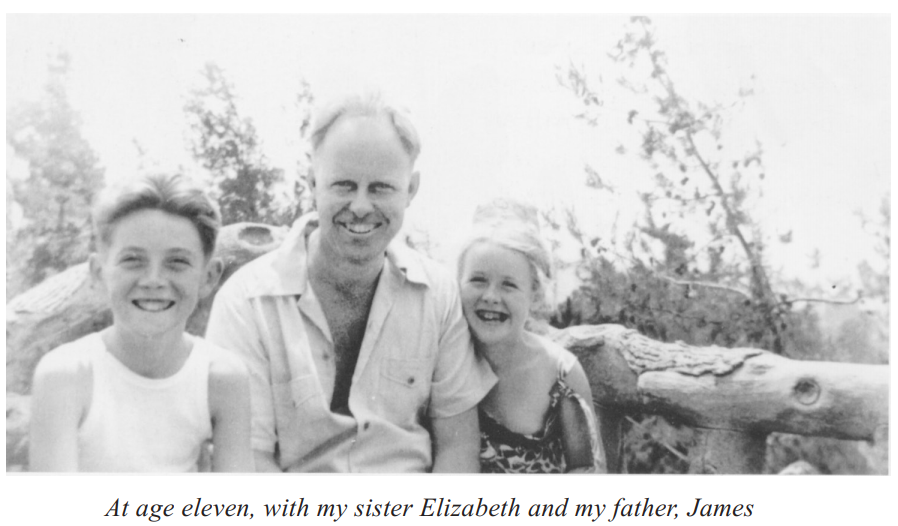
\includegraphics[width=0.75\linewidth]{image/Text5/Fig5.1.png}
\end{figure}

\noindent 4\\
The Hapsburgs added to their genetic woes by intermarrying. Arranging marriages between different branches of the Hapsburg clan and often among close relatives may have made political sense as a way of building alliances and ensuring dynastic succession, but it was anything but astute in genetic terms. Inbreeding of this kind can result in genetic disease, as the Hapsburgs found out to their cost. Charles II, the last of the Hapsburg monarchs in Spain, not only boasted a prize-worthy example of the family lip—he could not even chew his own food—but was also a complete invalid, and incapable, despite two marriages, of producing children.\\
哈布斯堡家族通过近亲结婚增加了他们的遗传问题。安排哈布斯堡家族不同分支之间,甚至经常是近亲之间的婚姻,可能在政治上有意义,作为建立联盟和确保王朝继承的一种方式,但在遗传学上却一点也不明智。这种近亲繁殖可能导致遗传疾病,哈布斯堡家族为此付出了代价。查理二世,西班牙哈布斯堡君主的最后一位,不仅拥有家族嘴唇的典型例子——他甚至不能咀嚼自己的食物——而且完全体弱多病,尽管有两次婚姻,却无法生育子女。\\

\noindent 5\\
Genetic disease has long stalked humanity. In some cases, such as Charles II’s, it has had a direct impact on history. Retrospective diagnosis has suggested that George III, the English king whose principal claim to fame is to have lost the American colonies in the Revolutionary War, suffered from an inherited disease, porphyria, which causes periodic bouts of madness. Some historians—mainly British ones—have argued that it was the distraction caused by George’s illness that permitted the Americans’ against-the-odds military success. While most hereditary diseases have no such geopolitical impact, they nevertheless have brutal and often tragic consequences for the afflicted families, sometimes for many generations. Understanding genetics is not just about understanding why we look like our parents. It is also about coming to grips with some of humankind’s oldest enemies: the flaws in our genes that cause genetic disease.\\
遗传病长期以来一直困扰着人类。在某些情况下,比如查理二世,它对历史产生了直接影响。回顾性诊断表明,乔治三世,这位以在独立战争中失去美国殖民地而闻名的英国国王,患有一种遗传病——卟啉症,这会导致周期性的疯狂发作。一些历史学家——主要是英国人——认为,正是乔治的疾病引起的分心,使得美国人取得了出人意料的军事成功。虽然大多数遗传病没有这样的地缘政治影响,但它们对受影响的家庭仍然有着残酷且往往悲惨的后果,有时甚至影响几代人。理解遗传学不仅仅是理解我们为什么长得像父母。它还涉及到与人类最古老的敌人之一——导致遗传病的基因缺陷——作斗争。\\

\noindent 6\\
Our ancestors must have wondered about the workings of heredity as soon as evolution endowed them with brains capable of formulating the right kind of question. And the readily observable principle that close relatives tend to be similar can carry you a long way if, like our ancestors, your concern with the application of genetics is limited to practical matters like improving domesticated animals (for, say, milk yield in cattle) and plants (for, say, the size of fruit). Generations of careful selection—breeding initially to domesticate appropriate species, and then breeding only from the most productive cows and from the trees with the largest fruit—resulted in animals and plants tailor-made for human purposes. Underlying this enormous unrecorded effort is that simple rule of thumb: that the most productive cows will produce highly productive offspring and from the seeds of trees with large fruit large-fruited trees will grow. Thus, despite the extraordinary advances of the past hundred years or so, the twentieth and twenty-first centuries by no means have a monopoly on genetic insight. Although it wasn’t until 1909 that the British biologist William Bateson gave the science of inheritance a name, genetics, and although the DNA revolution has opened up new and extraordinary vistas of potential progress, in fact the single greatest application of genetics to human well-being was carried out eons ago by anonymous ancient farmers. Almost everything we eat—cereals, fruit, meat, dairy products—is the legacy of that earliest and most far-reaching application of genetic manipulations to human problems.\\
我们的祖先一定在进化赋予他们能够提出正确问题的能力时,就对遗传的运作感到好奇。并且,近亲往往相似这一容易观察到的原则,如果像我们的祖先一样,你对遗传学的应用仅限于实际问题,如改善家养动物(例如,提高牛的产奶量)和植物(例如,增大水果的大小),那么这一原则可以带你走得很远。几代人的精心选择——最初是为了驯化合适的物种,然后只从产奶量最高的奶牛和果实最大的树上进行繁殖——结果产生了为人类目的量身定制的动物和植物。在这一巨大未记录的努力背后,是那条简单的经验法则:产奶量最高的奶牛将产生高生产力的后代,而从大果树木的种子中将生长出大果树木。因此,尽管在过去一百年左右的时间里取得了非凡的进步,但二十世纪和二十一世纪并不意味着对遗传学洞察力的垄断。尽管直到1909年,英国生物学家威廉·贝特森才给遗传学命名,尽管DNA革命开辟了新的、非凡的潜在进步视野,但实际上,对人类福祉的最大遗传学应用是由匿名的古代农民在很久以前进行的。我们吃的几乎所有东西——谷物、水果、肉类、乳制品——都是对人类问题最早和最深远的遗传操作应用的遗产。\\

\noindent 7\\
An understanding of the actual mechanics of genetics proved a tougher nut to crack. Gregor Mendel (1822–1884) published his famous paper on the subject in 1866 (and it was ignored by the scientific community for another thirty-four years). Why did it take so long? After all, heredity is a major aspect of the natural world, and, more important, it is readily, and universally, observable: a dog owner sees how a cross between a brown and black dog turns out, and all parents consciously or subconsciously track the appearance of their own characteristics in their children. One simple reason is that genetic mechanisms turn out to be complicated. Mendel’s solution to the problem is not intuitively obvious: children are not, after all, simply a blend of their parents’ characteristics. Perhaps most important was the failure by early biologists to distinguish between two fundamentally different processes, heredity and development. Today we understand that a fertilized egg contains the genetic information, contributed by both parents, that determines whether someone will be afflicted with, say, porphyria. That is heredity. The subsequent process, the development of a new individual from that humble starting point of a single cell, the fertilized egg, involves implementing that information. Broken down in terms of academic disciplines, genetics focuses on the information and developmental biology focuses on the use of that information. Lumping heredity and development together into a single phenomenon, early scientists never asked the questions that might have steered them toward the secret of heredity. Nevertheless, the effort had been under way in some form since the dawn of Western history.\\
对遗传学实际机制的理解证明是一个更难破解的难题。格雷戈尔·孟德尔(1822-1884)在1866年发表了他关于这个主题的著名论文(但科学界又忽视了另外三十四年)。为什么花了这么长时间?毕竟,遗传是自然界的一个主要方面,而且更重要的是,它是容易和普遍可观察的:狗的主人可以看到棕色和黑色狗的杂交结果,所有的父母都会有意或无意地追踪自己特征在孩子身上的表现。一个简单的原因是遗传机制结果很复杂。孟德尔对这个问题的解决方案并不直观明显:毕竟,孩子们并不是简单地混合了他们父母的特征。也许最重要的是早期生物学家未能区分两个根本不同的过程,遗传和发育。今天我们知道,受精卵包含了双方父母贡献的遗传信息,这些信息决定了某人是否会患有例如卟啉症。这就是遗传。随后的过程,即从单个细胞——受精卵这一谦卑的起点发展成一个新的个体,涉及实施这些信息。从学术学科的角度来看,遗传学专注于信息,而发育生物学专注于使用这些信息。将遗传和发育合并为一个单一现象,早期科学家从未提出可能引导他们揭开遗传秘密的问题。然而,这种努力自西方历史黎明以来就以某种形式进行着。\\

\noindent 8\\
The Greeks, including Hippocrates, pondered heredity. They devised a theory of “pangenesis,” which claimed that sex involved the transfer of miniaturized body parts: “Hairs, nails, veins, arteries, tendons and their bones, albeit invisible as their particles are so small. While growing, they gradually separate from each other.” This idea enjoyed a brief renaissance when Charles Darwin, desperate to support his theory of evolution by natural selection with a viable hypothesis of inheritance, put forward a modified version of pangenesis in the second half of the nineteenth century. In Darwin’s scheme, each organ—eyes, kidneys, bones—contributed circulating “gemmules” that accumulated in the sex organs, and were ultimately exchanged in the course of sexual reproduction. Because these gemmules were produced throughout an organism’s lifetime, Darwin argued any change that occurred in the individual after birth, like the stretch of a giraffe’s neck imparted by craning for the highest foliage, could be passed on to the next generation. Ironically, then, to buttress his theory of natural selection Darwin came to champion aspects of Jean-Baptiste Lamarck’s theory of inheritance of acquired characteristics—the very theory that his evolutionary ideas did so much to discredit. Darwin was invoking only Lamarck’s theory of inheritance; he continued to believe that natural selection was the driving force behind evolution, but supposed that natural selection operated on the variation produced by pangenesis. Had Darwin known about Mendel’s work (although Mendel published his results shortly after The Origin of Species appeared, Darwin was never aware of them), he might have been spared the embarrassment of this late-career endorsement of some of Lamarck’s ideas.\\
希腊人,包括希波克拉底,思考过遗传问题。他们提出了一种“泛生论”理论,声称性行为涉及微小化身体部位的转移:“头发、指甲、静脉、动脉、肌腱及其骨骼,尽管它们的颗粒非常小而看不见。在生长过程中,它们逐渐彼此分离。”当查尔斯·达尔文迫切希望用一个可行的遗传假设来支持他的自然选择进化论时,这个想法在十九世纪下半叶经历了短暂的复兴。在达尔文的方案中,每个器官——眼睛、肾脏、骨骼——都贡献了循环的“芽球”,这些芽球在性器官中积累,并最终在性繁殖过程中交换。由于这些芽球是在生物体的一生中产生的,达尔文认为任何在出生后发生的个体变化,如长颈鹿为了获取最高处的树叶而伸长脖子,都可以传递给下一代。具有讽刺意味的是,为了支持他的自然选择理论,达尔文开始支持让-巴蒂斯特·拉马克的获得性遗传特征理论的某些方面——正是他的进化思想极大地贬低了这一理论。达尔文只引用了拉马克的遗传理论;他继续相信自然选择是进化背后的驱动力,但认为自然选择作用于泛生论产生的变异。如果达尔文知道孟德尔的工作(尽管孟德尔在《物种起源》发表后不久就发表了他的结果,但达尔文从未了解过),他可能就不会因为晚年支持拉马克的一些观点而感到尴尬了。\\

\noindent 9\\
Whereas pangenesis supposed that embryos were assembled from a set of minuscule components, another approach, “preformationism,” avoided the assembly step altogether: either the egg or the sperm (exactly which was a contentious issue) contained a complete preformed individual called a homunculus. Development was therefore merely a matter of enlarging this into a fully formed being. In the days of preformationism, what we now recognize as genetic disease was variously interpreted: sometimes as a manifestation of the wrath of God or the mischief of demons and devils; sometimes as evidence of either an excess of or a deficit of the father’s “seed”; sometimes as the result of “wicked thoughts” on the part of the mother during pregnancy. On the premise that fetal malformation can result when a pregnant mother’s desires are thwarted, leaving her feeling stressed and frustrated, Napoleon passed a law permitting expectant mothers to shoplift. None of these notions, needless to say, did much to advance our understanding of genetic disease.\\
与泛生论认为胚胎是由一组微小的组成部分组装而成的不同,另一种方法“预成论”完全避免了组装步骤:无论是卵子还是精子(具体是哪一个是有争议的问题)都包含一个完整的预成个体,称为侏儒。因此,发育仅仅是将这个个体扩大成一个完全形成的生物体。在预成论的时代,我们现在所认识的遗传病被以各种方式解释:有时被认为是上帝的愤怒或恶魔和魔鬼的恶作剧的表现;有时被认为是父亲“种子”过多或不足的证据;有时被认为是母亲在怀孕期间“邪恶思想”的结果。基于孕妇的欲望受挫,感到压力和沮丧时可能导致胎儿畸形的前提,拿破仑通过了一项法律,允许孕妇偷窃。不用说,这些观点都没有对我们理解遗传病做出太多贡献。\\

\noindent 10\\
By the early nineteenth century, better microscopes had defeated preformationism. Look as hard as you like, you will never see a tiny homunculus curled up inside a sperm or egg cell. Pangenesis, though an earlier misconception, lasted rather longer—the argument would persist that the gemmules were simply too small to visualize—but was eventually laid to rest by August Weismann, who argued that inheritance depended on the continuity of germ plasm between generations and thus changes to the body over an individual's lifetime could not be transmitted to subsequent generations. His simple experiment involved cutting the tails off several generations of mice. According to Darwin's pangenesis, tailless mice would produce gemmules signifying "no tail" and so their offspring should develop a severely stunted hind appendage or none at all. When Weismann showed that the tail kept appearing after many generations of amputees, pangenesis bit the dust.\\
到了十九世纪初,更好的显微镜已经击败了预成论。无论你怎么努力看,你都不会在精子或卵细胞内看到一个蜷缩的小侏儒。泛生论虽然是一个早期的误解,但持续时间较长——争论会持续认为芽球太小而无法观察到——但最终被奥古斯特·魏斯曼平息,他认为遗传依赖于代际之间生殖质的连续性,因此个体一生中的身体变化不能传递给后代。他的简单实验包括切断几代老鼠的尾巴。根据达尔文的泛生论,无尾老鼠会产生表示“无尾”的芽球,因此它们的后代应该发育出严重发育不良的后肢或根本没有后肢。当魏斯曼表明即使在许多代截肢者之后尾巴仍然出现时,泛生论寿终正寝。\\

\begin{figure}
    \centering
    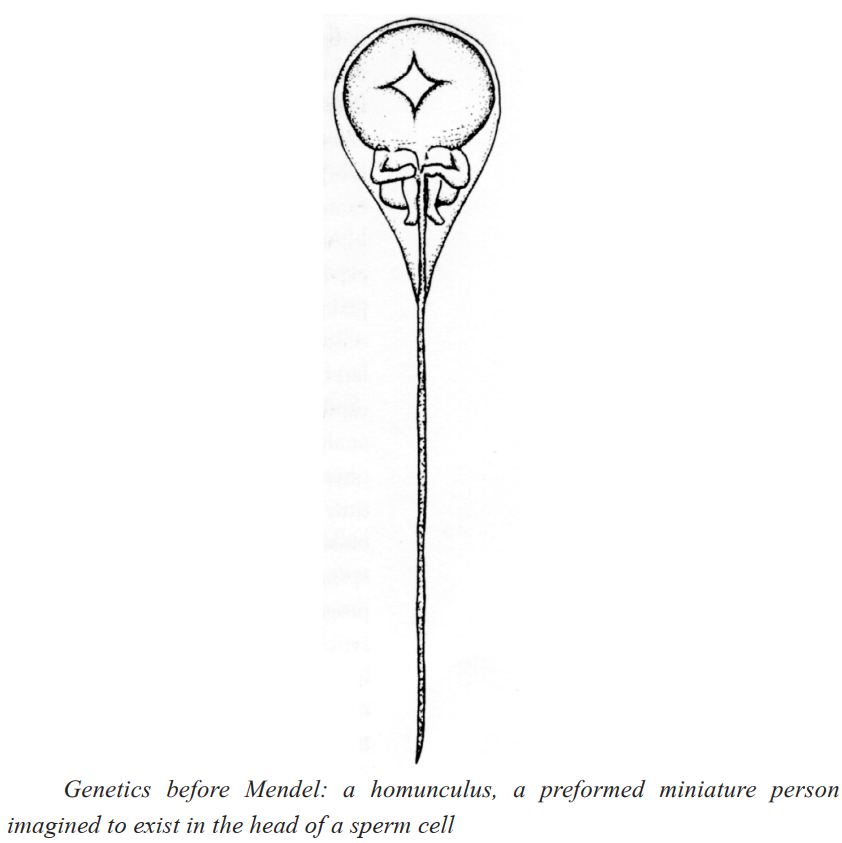
\includegraphics[width=0.75\linewidth]{image/Text5/Fig5.2.png}
\end{figure}

\noindent 11\\
Gregor Mendel was the one who got it right. By any standards, however, he was an unlikely candidate for scientific superstardom. Born to a farming family in what is now the Czech Republic, he excelled at the village school and, at twenty-one, entered the Augustinian monastery at Brünn. After proving a disaster as a parish priest—his response to the ministry was a nervous breakdown—he tried his hand at teaching. By all accounts he was a good teacher, but in order to qualify to teach a full range of subjects, he had to take an exam. He failed it. Mendel’s father superior, Abbot Napp, then dispatched him to the University of Vienna, where he was to bone up full-time for the retesting. Despite apparently doing well in physics at Vienna, Mendel again failed the exam, and so never rose above the rank of substitute teacher.\\
格雷戈尔·孟德尔是那个做对的人。然而,按照任何标准,他都是一个不太可能成为科学超级巨星的候选人。他出生在现在捷克共和国的一个农民家庭,在乡村学校表现出色,二十一岁时进入了布尔诺的奥古斯丁修道院。在证明作为教区牧师是个灾难后——他对牧师职务的反应是精神崩溃——他尝试了教学。据大家说,他是一位好老师,但为了有资格教授全部科目,他必须参加考试。他没有通过。孟德尔的上级,纳普修道院长,随后派他去维也纳大学,在那里他要全职准备重新考试。尽管在维也纳物理学似乎学得很好,孟德尔再次考试失败,因此从未超过代课教师的职位。\\

\noindent 12\\
Around 1856, at Abbot Napp's suggestion, Mendel undertook some scientific experiments on heredity. He chose to study a number of characteristics of the pea plants he grew in his own patch of the monastery garden. In 1865 he presented his results to the local natural history society in two lectures, and, a year later, published them in the society's journal. The work was a tour de force: the experiments were brilliantly designed and painstakingly executed, and his analysis of the results was insightful and deft. It seems that his training in physics contributed to his breakthrough because, unlike other biologists of that time, he approached the problem quantitatively. Rather than simply noting that crossbreeding of red and white flowers resulted in some red and some white offspring, Mendel actually counted them, realizing that the ratios of red to white progeny might be significant—as indeed they are. Despite sending copies of his article to various prominent scientists, Mendel found himself completely ignored by the scientific community. His attempt to draw attention to his results merely backfired. He wrote to his one contact among the ranking scientists of the day, botanist Karl Nägeli in Munich, asking him to replicate the experiments, and he duly sent off 140 carefully labeled packets of seeds. He should not have bothered. Nägeli believed that the obscure monk should be of service to him, rather than the other way around, so he sent Mendel seeds of his own favorite plant, hawkweed, challenging the monk to re-create his results with a different species. Sad to say, for various reasons, hawkweed is not well-suited to breeding experiments such as those Mendel had performed on the peas. The entire exercise was a waste of his time.\\
大约在1856年,在纳普修道院长的建议下,孟德尔进行了一些关于遗传的科学实验。他选择研究他在修道院花园里自己种植的豌豆植物的一些特性。1865年,他在当地自然历史学会的两次讲座中展示了他的结果,一年后,他将这些结果发表在学会的期刊上。这项工作是一次杰作:实验设计巧妙,执行精心,他对结果的分析富有洞察力和技巧。看来他在物理学方面的训练促成了他的突破,因为与其他当时的生物学家不同,他量化地处理了这个问题。孟德尔并没有简单地注意到红花和白花的杂交产生了一些红花和一些白花的后代,而是实际进行了计数,意识到红白后代的比例可能很重要——实际上确实如此。尽管他将文章的副本寄给了多位著名科学家,孟德尔发现自己完全被科学界忽视。他试图引起人们对他结果的关注,但只是适得其反。他写信给他那个时代排名靠前的科学家之一,慕尼黑的植物学家卡尔·纳格利,请求他复制实验,他也确实寄出了140包仔细标记的种子。他本不应该费心。纳格利认为这位默默无闻的修士应该为他服务,而不是反过来,所以他给孟德尔寄去了他自己最喜欢的植物——鹰爪草的种子,挑战这位修士用不同的物种重现他的结果。遗憾的是,由于各种原因,鹰爪草并不适合进行孟德尔在豌豆上进行的那种繁殖实验。整个练习都是浪费时间。\\

\noindent 13\\
Mendel’s low-profile existence as monk-teacher-researcher ended abruptly in 1868 when, on Napp’s death, he was elected abbot of the monastery. Although he continued his research—increasingly on bees and the weather—administrative duties were a burden, especially as the monastery became embroiled in a messy dispute over back taxes. Other factors, too, hampered him as a scientist. Portliness eventually curtailed his fieldwork: as he wrote, hill climbing had become “very difficult for me in a world where universal gravitation prevails.” His doctors prescribed tobacco to keep his weight in check, and he obliged them by smoking twenty cigars a day, as many as Winston Churchill. It was not his lungs, however, that let him down: in 1884, at the age of sixty-one, Mendel succumbed to a combination of heart and kidney disease.\\
孟德尔作为修士、教师和研究者的低调生活因纳普去世而在1868年突然结束,他被选为修道院的院长。尽管他继续他的研究——越来越多地涉及蜜蜂和天气——但行政职责成为了负担,特别是当修道院卷入了一场关于欠税的混乱纠纷时。其他因素也阻碍了他作为科学家的工作。最终,肥胖限制了他的实地工作:正如他所写,在普遍引力盛行的世界中,爬山对我来说变得“非常困难”。他的医生开处方让他吸烟以控制体重,他遵从医嘱每天吸二十支雪茄,和温斯顿·丘吉尔一样多。然而,让他倒下的不是他的肺:1884年,61岁的孟德尔因心脏和肾脏疾病去世。\\

\noindent 14\\
Not only were Mendel’s results buried in an obscure journal, but they would have been unintelligible to most scientists of the era. He was far ahead of his time with his combination of careful experiment and sophisticated quantitative analysis. Little wonder, perhaps, that it was not until 1900 that the scientific community caught up with him. The rediscovery of Mendel’s work, by three plant geneticists interested in similar problems, provoked a revolution in biology. At last the scientific world was ready for the monk’s peas.\\
孟德尔的结果不仅被埋没在一个鲜为人知的期刊中,而且对那个时代的大多数科学家来说是无法理解的。他以其精心的实验和复杂的定量分析远远超前于他的时代。也许不足为奇的是,直到1900年科学界才赶上他。三位对类似问题感兴趣的植物遗传学家重新发现了孟德尔的工作,引发了生物学领域的一场革命。终于,科学界准备好接受这位修道士的豌豆了。\\

\noindent 15\\
Mendel realized that there are specific factors—later to be called “genes”—that are passed from parent to offspring. He worked out that these factors come in pairs and that the offspring receives one from each parent.\\
孟德尔意识到有一些特定的因素——后来被称为“基因”——是从父母传给后代的。他推算出这些因素是成对出现的,后代从每个父母那里各继承一个。\\

\noindent 16\\
Noticing that peas came in two distinct colors, green and yellow, he deduced that there were two versions of the pea-color gene. A pea has to have two copies of the G version if it is to become green, in which case we say that it is GG for the pea-color gene. It must therefore have received a G pea-color gene from both of its parents. However, yellow peas can result both from YY and YG combinations. Having only one copy of the Y version is sufficient to produce yellow peas. Y trumps G. Because in the YG case the Y signal dominates the G signal, we call Y “dominant.” The subordinate G version of the pea-color gene is called “recessive.”\\
他注意到豌豆有两种明显的颜色,绿色和黄色,他推断豌豆颜色基因有两个版本。如果豌豆要变成绿色,它必须有两个G版本的副本,我们称其为豌豆颜色基因的GG。因此,它必须从两个父母那里各获得一个G颜色基因。然而,黄色豌豆可以由YY和YG组合产生。只要有一个Y版本的副本就足以产生黄色豌豆。Y优于G。因为在YG的情况下,Y信号支配G信号,我们称Y为“显性”。从属的G版本的豌豆颜色基因被称为“隐性”。\\

\noindent 17\\
Each parent pea plant has two copies of the pea-color gene, yet it contributes only one copy to each offspring; the other copy is furnished by the other parent. In plants, pollen grains contain sperm cells—the male contribution to the next generation—and each sperm cell contains just one copy of the pea-color gene. A parent pea plant with a YG combination will produce sperm that contain either a Y version or a G one. Mendel discovered that the process is random: 50 percent of the sperm produced by that plant will have a Y and 50 percent will have a G.\\
每个亲本豌豆植物都有两个豌豆颜色基因的副本,但它只向每个后代贡献一个副本;另一个副本由另一个亲本提供。在植物中,花粉粒包含精子细胞——对下一代的雄性贡献——每个精子细胞只包含一个豌豆颜色基因的副本。具有YG组合的亲本豌豆植物将产生包含Y版本或G版本的精子。孟德尔发现这个过程是随机的:该植物产生的精子中有50\%带有Y,50\%带有G。\\

\noindent 18\\
Suddenly many of the mysteries of heredity made sense. Characteristics, like the Hapsburg Lip, that are transmitted with a high probability (actually 50 percent) from generation to generation are dominant. Other characteristics that appear in family trees much more sporadically, often skipping generations, may be recessive. When a gene is recessive an individual has to have two copies of it for the corresponding trait to be expressed. Those with one copy of the gene are carriers: they don’t themselves exhibit the characteristic, but they can pass the gene on. Albinism, in which the body fails to produce pigment so the skin and hair are strikingly white, is an example of a recessive characteristic that is transmitted in this way. Therefore, to be albino you have to have two copies of the gene, one from each parent. (This was the case with the Reverend Dr. William Archibald Spooner, who was also—perhaps only by coincidence—prone to a peculiar form of linguistic confusion whereby, for example, “a well-oiled bicycle” might become “a well-boiled icicle.” Such reversals would come to be termed “spoonerisms” in his honor.) Your parents, meanwhile, may have shown no sign of the gene at all. If, as is often the case, each has only one copy, then they are both carriers. The trait has skipped at least one generation.\\
突然间,许多遗传的奥秘变得有意义了。像哈布斯堡唇这样以高概率(实际上是50\%)代代相传的特征是显性的。其他在家族树中更零星出现的特征,经常跳过几代,可能是隐性的。当一个基因是隐性的时,个体必须拥有两个副本才能表现出相应的特征。拥有一个基因副本的人是携带者:他们自己不表现出特征,但可以传递基因。白化病,即身体无法产生色素,导致皮肤和头发异常白皙,就是这样一种隐性特征的例子。因此,要成为白化病患者,你必须拥有两个基因副本,每个父母各提供一个。(这与威廉·阿奇博尔德·斯波纳牧师的情况相同,他也可能只是巧合地容易犯一种特殊的语言混淆错误,例如,“a well-oiled bicycle”可能会变成“a well-boiled icicle”。这种颠倒会以他的名字被称为“斯波纳现象”。)与此同时,你的父母可能根本没有表现出基因的迹象。如果情况经常是这样,每个父母只有一个副本,那么他们都是携带者。该特征至少跳过了一代。\\

\noindent 19\\
Mendel’s results implied that things—material objects—were transmitted from generation to generation. But what was the nature of these things?\\
孟德尔的结果暗示了一些东西——物质对象——是从一代传给下一代的。但这些东西的本质是什么?\\

\noindent 20\\
At about the time of Mendel’s death in 1884, scientists using ever-improving optics to study the minute architecture of cells coined the term “chromosome” to describe the long stringy bodies in the cell nucleus. But it was not until 1902 that Mendel and chromosomes came together.\\
大约在孟德尔1884年去世时,科学家们使用不断改进的光学技术研究细胞的微观结构,并创造了“染色体”一词来描述细胞核中的长丝状体。但直到1902年,孟德尔和染色体才联系在一起。\\

\begin{figure}
    \centering
    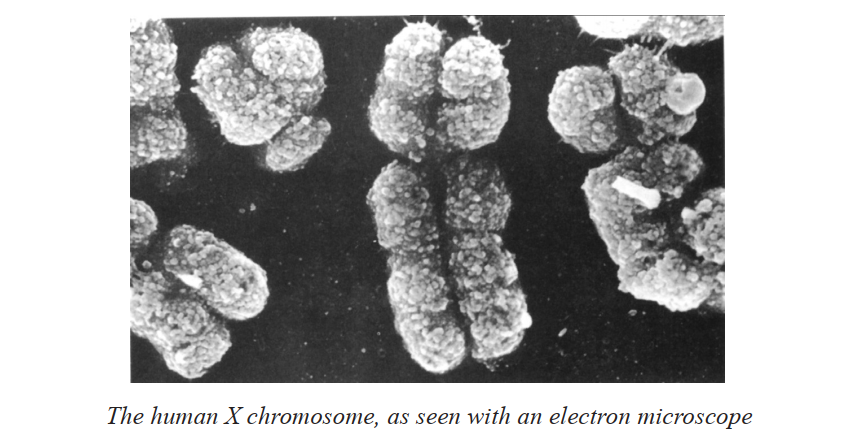
\includegraphics[width=0.75\linewidth]{image/Text5/Fig5.3.png}
\end{figure}

\noindent 21\\
A medical student at Columbia University, Walter Sutton, realized that chromosomes had a lot in common with Mendel’s mysterious factors. Studying grasshopper chromosomes, Sutton noticed that most of the time they are doubled up—just like Mendel’s paired factors. But Sutton also identified one type of cell in which chromosomes were not paired: the sex cells. Grasshopper sperm have only a single set of chromosomes, not a double set. This was exactly what Mendel had described: his pea plant sperm cells also only carried a single copy of each of his factors. It was clear that Mendel’s factors, now called genes, must be on the chromosomes.\\
哥伦比亚大学的一名医学生沃尔特·萨顿意识到染色体与孟德尔的神秘因素有很多共同之处。研究蚱蜢的染色体时,萨顿注意到大多数时候它们是成对出现的——就像孟德尔的配对因素一样。但萨顿也发现了一种染色体不成对的细胞类型:性细胞。蚱蜢精子只有一套染色体,而不是两套。这正是孟德尔所描述的:他的豌豆植物精子细胞也只携带每个因素的一个副本。很明显,孟德尔的因素,现在被称为基因,一定位于染色体上。\\

\noindent 22\\
In Germany Theodor Boveri independently came to the same conclusions as Sutton, and so the biological revolution their work had precipitated came to be called the Sutton-Boveri chromosome theory of inheritance. Suddenly genes were real. They were on chromosomes, and you could actually see chromosomes through the microscope.\\
在德国,西奥多·博韦里独立地得出了与萨顿相同的结论,因此他们工作引发的生物学革命被称为萨顿-博韦里染色体遗传理论。突然间,基因变得真实存在。它们位于染色体上,你实际上可以通过显微镜看到染色体。\\

\noindent 23\\
Not everyone bought the Sutton-Boveri theory. One skeptic was Thomas Hunt Morgan, also at Columbia. Looking down the microscope at those stringy chromosomes, he could not see how they could account for all the changes that occur from one generation to the next. If all the genes were arranged along chromosomes, and all chromosomes were transmitted intact from one generation to the next, then surely many characteristics would be inherited together. But since empirical evidence showed this not to be the case, the chromosomal theory seemed insufficient to explain the variation observed in nature. Being an astute experimentalist, however, Morgan had an idea how he might resolve such discrepancies. He turned to the fruit fly, Drosophila melanogaster, the drab little beast that, ever since Morgan, has been so beloved by geneticists.\\
并不是每个人都接受萨顿-博韦里理论。一位怀疑论者是哥伦比亚大学的托马斯·亨特·摩根。通过显微镜观察那些细长的染色体,他无法理解它们如何解释一代代之间发生的变化。如果所有的基因都排列在染色体上,并且所有染色体都完整地从一代传给下一代,那么许多特征肯定会一起遗传。但由于经验证据表明事实并非如此,染色体理论似乎不足以解释自然界中观察到的变异。然而,作为一个敏锐的实验家,摩根有了一个解决这些差异的想法。他转向了果蝇,黑腹果蝇,这种不起眼的小生物,自从摩根以来,一直受到遗传学家的喜爱。\\

\begin{figure}
    \centering
    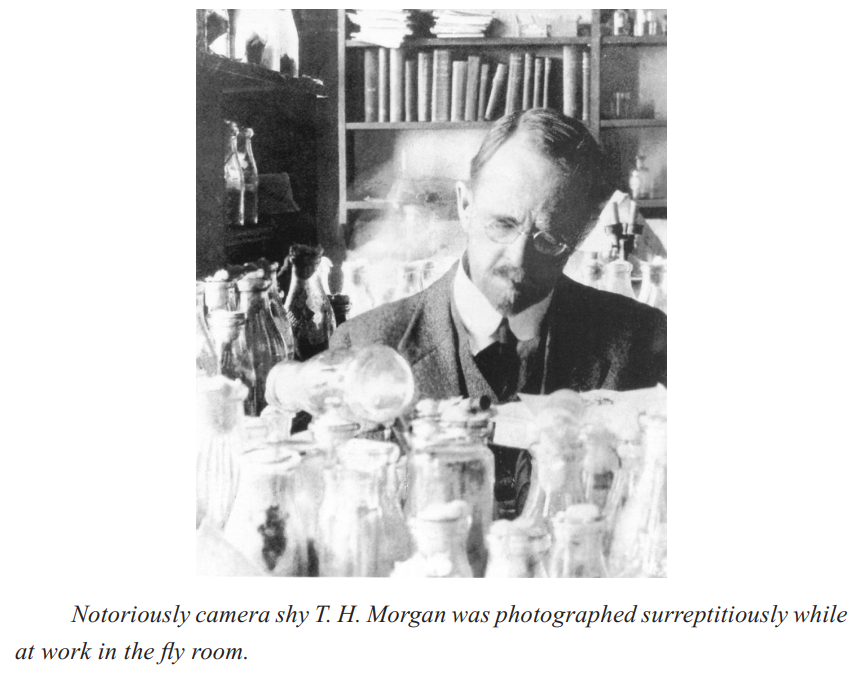
\includegraphics[width=0.75\linewidth]{image/Text5/Fig5.4.png}
\end{figure}

\noindent 24\\
In fact, Morgan was not the first to use the fruit fly in breeding experiments—that distinction belonged to a lab at Harvard that first put the critter to work in 1901—but it was Morgan’s work that put the fly on the scientific map. Drosophila is a good choice for genetic experiments. It is easy to find (as anyone who has left out a bunch of overripe bananas during the summer well knows); it is easy to raise (bananas will do as feed); and you can accommodate hundreds of flies in a single milk bottle (Morgan’s students had no difficulty acquiring milk bottles, pinching them at dawn from doorsteps in their Manhattan neighborhood); and it breeds and breeds (a whole generation takes about ten days, and each female lays several hundred eggs). Starting in 1907 in a famously squalid, cockroach-infested, banana-stinking lab that came to be known affectionately as the “fly room,” Morgan and his students (“Morgan’s boys” as they were called) set to work on fruit flies.\\
事实上,摩根并不是第一个在育种实验中使用果蝇的人——这一荣誉属于1901年首次让果蝇工作的哈佛大学实验室——但正是摩根的工作让果蝇在科学界声名鹊起。果蝇是遗传实验的好选择。它很容易找到(任何在夏天留下一堆过熟香蕉的人都知道);它很容易饲养(香蕉可以作为食物);你可以在一只牛奶瓶中容纳数百只果蝇(摩根的学生在曼哈顿的家门口轻松地获取牛奶瓶);而且它繁殖迅速(整个一代大约需要十天,每只雌性产下数百个卵)。从1907年开始,在一个以肮脏、蟑螂成灾、香蕉味弥漫而闻名的实验室里,这个实验室后来被亲切地称为“果蝇室”,摩根和他的学生们(他们被称为“摩根的男孩”)开始研究果蝇。\\

\noindent 25\\
Unlike Mendel, who could rely on the variant strains isolated over the years by farmers and gardeners—yellow peas as opposed to green ones, wrinkled skin as opposed to smooth—Morgan had no menu of established genetic differences in the fruit fly to draw upon. And you cannot do genetics until you have isolated some distinct characteristics to track through the generations. Morgan’s first goal therefore was to find “mutants,” the fruit fly equivalents of yellow or wrinkled peas. He was looking for genetic novelties, random variations that somehow simply appeared in the population.\\
与孟德尔不同,孟德尔可以依靠农民和园丁多年来分离出的变种——黄色豌豆与绿色豌豆相对,皱皮与光滑皮相对——摩根没有现成的果蝇遗传差异菜单可供参考。而且在你隔离出一些可以追踪几代的明显特征之前,你无法进行遗传学研究。因此,摩根的第一个目标是找到“突变体”,即果蝇中的黄色或皱皮豌豆的等价物。他正在寻找遗传新奇性,即随机变异,这些变异不知何故地出现在种群中。\\

\noindent 26\\
One of the first mutants Morgan observed turned out to be one of the most instructive. While normal fruit flies have red eyes, these had white ones. And he noticed that the white-eyed flies were typically male. It was known that the sex of a fruit fly—or, for that matter, the sex of a human—is determined chromosomally: females have two copies of the X chromosome, whereas males have one copy of the X and one copy of the much smaller Y. In light of this information, the white-eye result suddenly made sense: the eye-color gene is located on the X chromosome and the white-eye mutation, W, is recessive. Because males have only a single X chromosome, even recessive genes, in the absence of a dominant counterpart to suppress them, are automatically expressed. White-eyed females were relatively rare because they typically had only one copy of W so they expressed the dominant red eye color. By correlating a gene—the one for eye color—with a chromosome, the X, Morgan, despite his initial reservations, had effectively proved the Sutton-Boveri theory. He had also found an example of “sex-linkage,” in which a particular characteristic is disproportionately represented in one sex.\\
摩根观察到的第一个突变体之一结果是最有启发性的。正常的果蝇有红色的眼睛,而这些果蝇有白色的眼睛。他注意到白眼果蝇通常是雄性。已知果蝇或人类的性别是由染色体决定的:雌性有两个X染色体的副本,而雄性有一个X和一个较小的Y。根据这些信息,白眼结果突然变得有意义:眼色基因位于X染色体上,白眼突变W是隐性的。因为雄性只有一个X染色体,即使是隐性基因,在没有显性对应基因来抑制它们的情况下,也会自动表现出来。白眼雌性相对较少,因为它们通常只有一个W副本,所以表现出显性的红色眼睛。通过将一个基因——眼色基因——与X染色体相关联,摩根尽管最初有所保留,但有效地证明了萨顿-博韦里理论。他还发现了一个“性连锁”的例子,其中一个特定特征在一个性别中不成比例地表现出来。\\

\noindent 27\\
Like Morgan’s fruit flies, Queen Victoria provides a famous example of sex-linkage. On one of her X chromosomes, she had a mutated gene for hemophilia, the “bleeding disease” in whose victims proper blood clotting fails to occur. Because her other copy was normal, and the hemophilia gene is recessive, she herself did not have the disease. But she was a carrier. Her daughters did not have the disease either; evidently each possessed at least one copy of the normal version. But Victoria’s sons were not all so lucky. Like all males (fruit fly males included), each had only one X chromosome; this was necessarily derived from Victoria (a Y chromosome could have come only from Prince Albert, Victoria’s husband). Because Victoria had one mutated copy and one normal copy, each of her sons had a 50-50 chance of having the disease. Prince Leopold drew the short straw: he developed hemophilia, and died at thirty-one, bleeding to death after a minor fall. Two of Victoria’s daughters, Princesses Alice and Beatrice, were carriers, having inherited the mutated gene from their mother. They each produced carrier daughters and sons with hemophilia. Alice’s grandson Alexis, heir to the Russian throne, had hemophilia, and would doubtless have died young had the Bolsheviks not gotten to him first.\\
像摩根的果蝇一样,维多利亚女王提供了性连锁的一个著名例子。在她的一条X染色体上,她有一个血友病的突变基因,这是一种“出血病”,患者的正常凝血无法发生。因为她的另一个副本是正常的,而且血友病基因是隐性的,她自己并没有这种疾病。但她是一个携带者。她的女儿们也没有这种疾病;显然每人至少拥有一个正常版本的副本。但维多利亚的儿子们并不都那么幸运。像所有雄性(包括果蝇雄性)一样,他们每人只有一个X染色体;这必然来自维多利亚(Y染色体只能来自维多利亚的丈夫阿尔伯特亲王)。因为维多利亚有一个突变副本和一个正常副本,她的每个儿子都有50-50的几率患病。利奥波德王子不幸中招:他患了血友病,在一次轻微摔倒后因出血过多而死,年仅31岁。维多利亚的两个女儿,爱丽丝公主和比阿特丽斯公主,是携带者,她们从母亲那里继承了突变基因。她们各自生下了携带者女儿和患有血友病的儿子。爱丽丝的孙子,俄罗斯王位继承人阿列克谢,患有血友病,如果不是布尔什维克人先找到他,他无疑会早逝。\\

\noindent 28\\
Morgan's fruit flies had other secrets to reveal. In the course of studying genes located on the same chromosome, Morgan and his students found that chromosomes actually break apart and re-form during the production of sperm and egg cells. This meant that Morgan's original objections to the Sutton-Boveri theory were unwarranted: the breaking and re-forming—“recombination,” in modern genetic parlance—shuffles gene copies between members of a chromosome pair. This means that, say, the copy of chromosome 12 I got from my mother (the other, of course, comes from my father) is in fact a mix of my mother’s two copies of chromosome 12, one of which came from her mother and one from her father. Her two 12s recombined—exchanged material—during the production of the egg cell that eventually turned into me. Thus my maternally derived chromosome 12 can be viewed as a mosaic of my grandparents’ 12s. Of course, my mother's maternally derived 12 was itself a mosaic of her grandparents’ 12s, and so on.\\
摩根的果蝇还有其他秘密要揭示。在研究位于同一染色体上的基因的过程中,摩根和他的学生发现染色体实际上在精子和卵细胞的生产过程中会分离并重新形成。这意味着摩根对萨顿-博韦里理论的最初反对是没有根据的:现代遗传学中所说的“重组”——即在染色体对成员之间洗牌基因副本——是成立的。这意味着,比如说,我从母亲那里得到的第12号染色体的副本实际上是我母亲两个第12号染色体副本的混合,其中一个来自她的母亲的,一个来自她的父亲。她的两个第12号染色体在形成最终变成我的卵细胞过程中重新组合——交换了物质。因此,我母亲遗传给我的第12号染色体可以看作是我祖父母的第12号染色体的马赛克。当然,我母亲从她母亲那里遗传的第12号染色体本身也是她祖父母的第12号染色体的马赛克,以此类推。\\

\noindent 29\\
Recombination permitted Morgan and his students to map out the positions of particular genes along a given chromosome. Recombination involves breaking (and re-forming) chromosomes. Because genes are arranged like beads along a chromosome string, a break is statistically much more likely to occur between two genes that are far apart (with more potential break points intervening) on the chromosome than between two genes that are close together. If, therefore, we see a lot of reshuffling for any two genes on a single chromosome, we can conclude that they are a long way apart; the rarer the reshuffling, the closer the genes likely are. This basic and immensely powerful principle underlies all of genetic mapping. One of the primary tools of scientists involved in the Human Genome Project and of researchers at the forefront of the battle against genetic disease was thus developed all those years ago in the filthy, cluttered Columbia fly room. Each new headline in the science section of the newspaper these days along the lines of “Gene for Something Located” is a tribute to the pioneering work of Morgan and his boys.\\
重组使摩根和他的学生能够绘制出特定基因在给定染色体上的位置。重组涉及断裂(和重新形成)染色体。由于基因像珠子一样排列在染色体串上,断裂在统计上更有可能发生在染色体上相距较远的两个基因之间(有更多的潜在断裂点),而不是发生在相距较近的两个基因之间。因此,如果在单个染色体上的任意两个基因之间我们看到了大量的重组,我们可以得出结论,它们相距很远;重组越少,基因可能越近。这一基本而强大的原则支撑着所有的基因图谱系。参与人类基因组计划的科学家和在与遗传病作斗争的研究人员的主要工具之一,就是多年前在杂乱的哥伦比亚果蝇室中开发的。如今报纸科学版上的每一个“基因定位于某物”的新标题都是对摩根和他的学生们开创性工作的致敬。\\

\noindent 30\\
The rediscovery of Mendel’s work, and the breakthroughs that followed it, sparked a surge of interest in the social significance of genetics. While scientists had been grappling with the precise mechanisms of heredity through the eighteenth and nineteenth centuries, public concern had been mounting about the burden placed on society by what came to be called the “degenerate classes”—the inhabitants of poorhouses, workhouses, and insane asylums. What could be done with these people? It remained a matter of controversy whether they should be treated charitably—which, the less charitably inclined claimed, ensured such folk would never exert themselves and would therefore remain forever dependent on the largesse of the state or of private institutions—or whether they should be simply ignored, which, according to the charitably inclined, would result only in perpetuating the inability of the unfortunate to extricate themselves from their blighted circumstances.\\
孟德尔工作的重新发现以及随之而来的突破,引发了人们对遗传学社会意义的兴趣激增。虽然科学家们一直在努力解决十八和十九世纪遗传的精确机制,公众对所谓的“退化阶级”——贫民窟、济贫民院和精神病院的居民——给社会带来的负担感到担忧。应该如何处理这些人?他们是否应该得到慈善对待——不那么慈善的人声称,这确保了这些人永远不会努力,因此将永远依赖国家或私人机构的慷慨——还是应该被忽视,根据慈善倾向的人说,这只会使不幸者无法摆脱他们悲惨的处境遇。\\

\noindent 31\\
The publication of Darwin’s Origin of Species in 1859 brought these issues into sharp focus. Although Darwin carefully omitted to mention human evolution, fearing that to do so would only further inflame an already raging controversy, it required no great leap of imagination to apply his idea of natural selection to humans. Natural selection is the force that determines the fate of all genetic variations in nature—mutations like the one Morgan found in the fruit fly eye-color gene, but also perhaps differences in the abilities of human individuals to fend for themselves.\\
达尔文的《物种起源》在1859年出版,使这些问题成为焦点。尽管达尔文小心翼翼地避免提及人类进化,担心这样做只会进一步激化已经激烈的争议,但将他的自然选择理论应用于人类并不需要很大的想象力。自然选择是决定自然界所有遗传变异命运的力量——像摩根在果蝇眼色基因中发现的突变,但也许还有人类个体自卫能力的差异。\\

\noindent 32\\
Natural populations have an enormous reproductive potential. Take fruit flies, with their generation time of just ten days, and females that produce some three hundred eggs apiece (half of which will be female): starting with a single fruit fly couple, after a month (i.e., three generations later), you will have 150 × 150 × 150 × 150 fruit flies on your hands—that’s more than 3 million flies, all of them derived from just one pair in just one month. Darwin made the point by choosing a species from the other end of the reproductive spectrum:\\
自然种群具有巨大的繁殖潜力。以果蝇为例,它们的繁殖周期仅为十天,雌性每次产卵约三百个(其中一半将是雌性):从一对果蝇开始,一个月(即三代之后),你将拥有150 × 150 × 150只果蝇——这超过300万只果蝇,它们都源自一个月前的那一对果蝇。达尔文通过选择繁殖谱系另一端的物种来说明这一点:\\

\addtolength{\leftskip}{1cm}

The elephant is reckoned to be the slowest breeder of all known animals, and I have taken some pains to estimate its probable minimum rate of natural increase: it will be under the mark to assume that it breeds when thirty years old, and goes on breeding till ninety years old, bringing forth three pairs of young in this interval; if this be so, at the end of the fifth century there would be alive fifteen million elephants, descended from the first pair.\\
大象被认为是所有已知动物中繁殖最慢的,我费了一些心思来估计它可能的最小自然增长率:假设它在30岁时繁殖,并一直繁殖到90岁,在这段时间内产下三对幼崽;如果这样的话,到第五个世纪末,将会有1500万头大象活着,它们都是最初那对大象的后代。\\

\addtolength{\leftskip}{-1cm}

\noindent 33\\
All these calculations assume that all the baby fruit flies and all the baby elephants make it successfully to adulthood. In theory, therefore, there must be an infinitely large supply of food and water to sustain this kind of reproductive overdrive. In reality, of course, those resources are limited, and not all baby fruit flies or baby elephants make it. There is competition among individuals within a species for those resources. What determines who wins the struggle for access to the resources? Darwin pointed out genetic variation means that some individuals have advantages in what he called “the struggle for existence.” To take the famous example of Darwin’s finches from the Galapagos Islands, those individuals with genetic advantages—like the right size of beak for eating the most abundant seeds—are more likely to survive and reproduce. So the advantageous genetic variant—having a bill the right size—tends up being passed on to the next generation. The result is that natural selection enriches the next generation with the beneficial mutation so that eventually, over enough generations, every member of the species ends up with that characteristic.\\
所有这些计算都假设所有的果蝇和所有的小象都能成功地长到成年。因此,理论上必须有无限量的食物和水来维持这种生殖过度繁殖。当然,在现实中,这些资源是有限的,并不是所有的果蝇或小象都能成功长大。物种内部个体之间对这些资源存在竞争。是什么决定了谁在资源争夺中获胜?达尔文指出,遗传变异意味着一些个体在所谓的“生存斗争”中具有优势。以达尔文在加拉帕戈斯群岛的雀鸟为例,那些具有遗传优势的个体——比如适合吃最丰富种子的喙的合适大小——更有可能生存和繁殖。因此,有利的遗传变异——喙的合适大小——往往会传给下一代。结果是自然选择使下一代获得有益的突变,这样最终,经过足够多的代,物种的每个成员都会拥有这种特征。\\

\noindent 34\\
The Victorians applied the same logic to humans. They looked around and were alarmed by what they saw. The decent, moral, hardworking middle classes were being massively outreproduced by the dirty, immoral, lazy lower classes. The Victorians assumed that the virtues of decency, morality, and hard work ran in families just as the vices of filth, wantonness, and indolence did. Such characteristics must then be hereditary; thus, to the Victorians, morality and immorality were merely two of Darwin’s genetic variants. And if the great unwashed were outreproducing the respectable classes, then the “bad” genes would be increasing in the human population. The species was doomed! Humans would gradually become more and more depraved as the “immorality” gene became more and more common.\\
维多利亚时代的人将同样的逻辑应用于人类。他们环顾四周,对他们所看到的感到震惊。体面、道德、勤奋的中产阶级被肮脏、不道德、懒惰的下层阶级大量繁殖。维多利亚人假设体面、道德和勤奋的美德就像肮脏、放荡和懒惰的恶习气一样在家族中遗传。这些特征一定是遗传的;因此,对维多利亚时代的人来说,道德和不道德仅仅是达尔文的两种遗传变体。如果伟大的不道德的人正在繁殖出有声望的阶级,那么“坏”基因将在人类种群中增加。人类注定要灭亡!随着“不道德”基因变得越来越普遍,人类将逐渐变得越来越堕落。\\

\noindent 35\\
Francis Galton had good reason to pay special attention to Darwin’s book, as the author was his cousin and friend. Darwin, some thirteen years older, had provided guidance during Galton’s rather rocky college experience. But it was The Origin of Species that would inspire Galton to start a social and genetic crusade that would ultimately have disastrous consequences. In 1883, a year after his cousin’s death, Galton gave the movement a name: eugenics.\\
弗朗西斯·高尔顿有充分的理由特别关注达尔文的书,因为作者是他的表亲和朋友。达尔文比他大十三岁,在高尔顿相当坎坷的大学经历中提供了指导。但正是《物种起源》激发了高尔顿发起一场社会和遗传运动,这场运动最终产生了灾难性的后果。1883年,即他表亲去世一年后,高尔顿给这场运动起了一个名字:优生学。\\

\noindent 36\\
Eugenics was only one of Galton’s many interests; Galton enthusiasts refer to him as a polymath, detractors as a dilettante. In fact, he made significant contributions to geography, anthropology, psychology, genetics, meteorology, statistics, and, by setting fingerprint analysis on a sound scientific footing, to crimin criminology. Born in 1822 into a prosperous family, his education—partly in medicine and partly in mathematics—was mostly a chronicle of defeated expectations. The death of his father when he was twenty-one simultaneously freed him from paternal restraint and yielded a handsome inheritance; the young man duly took advantage of both. After a full six years of being what might be described today as a trust-fund dropout, however, Galton settled down to become a productive member of the Victorian establishment. He made his name leading an expedition to a then little known region of southwest Africa in 1850-52. In his account of his explorations, we encounter the first instance of the one strand that connects his many varied interests: he counted and measured everything. Galton was only happy when he could reduce a phenomenon to a set of numbers.\\
优生学只是高尔顿的众多兴趣之一;高尔顿的爱好者称他为多面手,侦探小说家。事实上,他对地理、人类学、心理学、遗传学、气象学、统计学以及通过为指纹分析奠定科学基础的犯罪学都做出了重要贡献。1822年出生于一个富裕家庭,他的教育——部分是医学,部分是数学——大部分是未实现的期望。21岁时父亲的去世同时使他摆脱了父亲的束缚,并获得了一笔可观的遗产;年轻人充分利用了这两方面。然而,在经历了六年的“信托基金辍学者”生活后,高尔顿安定下来,成为维多利亚时代有生产力的成员。他在1850-52年领导了一次前往当时鲜为人知的西南非探险,使他声名鹊起。在他的探险记述中,我们遇到了将他的多种兴趣联系在一起的第一条线索:他计数和测量一切。高尔顿只有在能够将现象简化为一组数字时才感到高兴。\\

\noindent 37\\
At a missionary station he encountered a striking specimen of steatopygia—a condition of particularly protuberant buttocks, common among the indigenous Nama women of the region—and realized that this woman was naturally endowed with the figure that was then fashionable in Europe. The only difference was that it required enormous (and costly) ingenuity on the part of European dressmakers to create the desired “look” for their clients.\\
在一个传教站,他遇到了一个明显患有臀部脂肪过多症的人——这是一种臀部特别突出的情况,在该地区的纳马族原住民女性中很常见——他意识到,这个女人天生就拥有当时在欧洲流行的身材。唯一的区别在于,欧洲的裁缝们需要花费大量(且昂贵)的心思,才能为他们的客户打造出那种理想的 “造型” 。\\

\addtolength{\leftskip}{1cm}

I profess to be a scientific man, and was exceedingly anxious to obtain accurate measurements of her shape; but there was a difficulty in doing this. I did not know a word of Hottentot [the Dutch name for the Nama], and could never therefore have explained to the lady what the object of my footrule could be; and I really dared not ask my worthy missionary host to interpret for me. I therefore felt in a dilemma as I gazed at her form, that gift of bounteous nature to this favoured race, which no mantua-maker, with all her crinoline and stuffing, can do otherwise than humbly imitate. The object of my admiration stood under a tree, and was turning herself about to all points of the compass, as ladies who wish to be admired usually do. Of a sudden my eye fell upon my sextant; the bright thought struck me, and I took a series of observations upon her figure in every direction, up and down, crossways, diagonally, and so forth, and I registered them carefully upon an outline drawing for fear of any mistake; this being done, I boldly pulled out my measuring tape, and measured the distance from where I was to the place she stood, and having thus obtained both base and angles, I worked out the results by trigonometry and logarithms.\\
我自称是个科学工作者,极其渴望精确测量她的身形;但这做起来却有个困难。我对霍屯督语(荷兰人对纳马人的称呼)一窍不通,因此根本无法向那位女士解释我拿的直尺是用来做什么的;而且我实在不敢请我那可敬的传教士房东帮我翻译。因此,当我凝视着她的身形——大自然慷慨赐予这个得天独厚的种族的礼物,就连最出色的女装裁缝,用尽裙撑和衬垫,也只能谦卑地模仿——我感到左右为难。我欣赏的对象站在一棵树下,像那些渴望被人欣赏的女士们常做的那样,转动着身子,面向各个方向。突然,我的目光落在了六分仪上;我灵机一动,开始从各个方向,上下、横向、斜向等等,对她的身形进行一系列的观测,并小心翼翼地把观测结果标注在一张轮廓图上,生怕出错;完成这些后,我大胆地拿出卷尺,测量了我所在的位置到她站立之处的距离。这样,在得到了底边和角度的数据后,我运用三角学和对数算出了结果。\\

\addtolength{\leftskip}{-1cm}

\begin{figure}
    \centering
    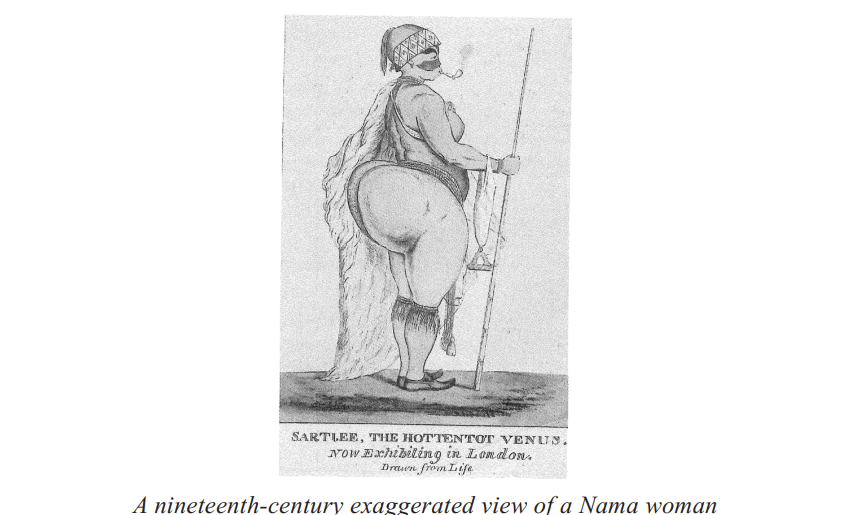
\includegraphics[width=0.75\linewidth]{image/Text5/Fig5.5.png}
\end{figure}

\noindent 38\\
Galton’s passion for quantification resulted in his developing many of the fundamental principles of modern statistics. It also yielded some clever observations. For example, he tested the efficacy of prayer. He figured that if prayer worked, those most prayed for should be at an advantage; to test the hypothesis he studied the longevity of British monarchs. Every Sunday, congregations in the Church of England following the Book of Common Prayer beseeched God to “Endue the king/queen plenteously with heavenly gifts; Grant him/her in health and wealth long to live.” Surely, Galton reasoned, the cumulative effect of all those prayers should be beneficial. In fact, prayer seemed ineffectual: he found that on average the monarchs died somewhat younger than other members of the British aristocracy.\\
高尔顿对量化的热衷促使他提出了现代统计学的许多基本原理。这也让他有了一些巧妙的观察。例如,他测试了祈祷的效果。他认为,如果祈祷有效,那些被人们最多地为之祈祷的人应该处于有利地位;为了验证这一假设,他研究了英国君主的寿命。每个星期天,英国国教的会众依照《公祷书》祈求上帝 “慷慨地赐予国王/女王属天的恩赐;赐予他/她健康和财富,使其长寿”。高尔顿推断,所有这些祈祷的累积效果肯定是有益的。事实上,祈祷似乎没有效果:他发现,平均而言,君主的寿命比英国贵族的其他成员要短一些 。\\

\noindent 39\\
Because of the Darwin connection—their common grandfather, Erasmus Darwin, too was one of the intellectual giants of his day—Galton was especially sensitive to the way in which certain lineages seemed to spawn disproportionately large numbers of prominent and successful people. In 1869 he published what would become the underpinning of all his ideas on eugenics, a treatise called *Hereditary Genius: An Inquiry into Its Laws and Consequences*. In it he purported to show that talent, like simple genetic traits such as the Hapsburg Lip, does indeed run in families; he recounted, for example, how some families had produced generation after generation of judges. His analysis largely neglected to take into account the effect of the environment: the son of a prominent judge is, after all, rather more likely to become a judge—by virtue of his father’s connections, if nothing else—than the son of a peasant farmer. Galton did not, however, completely overlook the effect of the environment, and it was he who first referred to the “nature/nurture” dichotomy, possibly in reference to Shakespeare’s irredeemable villain, Caliban, “a devil, a born devil, on whose nature/Nurture can never stick.”\\
由于与达尔文家族的关联——他们共同的祖父伊拉斯谟·达尔文也是他那个时代的知识巨匠之一——高尔顿对某些家族谱系中似乎不成比例地涌现出大量杰出成功人士的现象格外敏感。1869 年,他出版了一部论著《遗传的天才:对其规律和后果的探究》,这部著作成为了他所有优生学思想的基石。在书中,他试图证明,天赋如同哈布斯堡唇(一种简单的遗传特征)一样,确实在家族中代代相传;例如,他讲述了一些家族是如何一代又一代地出法官的。他的分析在很大程度上忽视了环境的影响:毕竟,一位杰出法官的儿子,即便没有其他因素,仅凭借父亲的人脉关系,也比农民的儿子更有可能成为法官。然而,高尔顿并没有完全忽视环境的影响,而且是他首次提出了 “先天/后天” 二分法,这可能是引用了莎士比亚笔下不可救药的反派角色凯列班的形象,“一个恶魔,天生的恶魔,后天教养对其本性毫无作用” 。\\

\noindent 40

\addtolength{\leftskip}{1cm}

\noindent The results of his analysis, however, left no doubt in Galton’s mind. \\
然而,他的分析结果让高尔顿坚信不疑。\\

\noindent I have no patience with the hypothesis occasionally expressed, and often implied, especially in tales written to teach children to be good, that babies are born pretty much alike, and that the sole agencies in creating differences between boy and boy, and man and man, are steady application and moral effort. It is in the most unqualified manner that I object to pretensions of natural equality.\\
我无法忍受那种偶尔被提及,且经常被暗示的假设,尤其是在教导孩子向善的故事中所表达的——婴儿出生时基本相似,而造成男孩与男孩之间、男人与男人之间差异的唯一因素,是坚持不懈的努力和道德上的修为。我毫无保留地反对这种关于天生平等的主张 。\\

\addtolength{\leftskip}{-1cm}

\noindent 41\\
A corollary of his conviction that these traits are genetically determined, he argued, was that it would be possible to “improve” the human stock by preferentially breeding gifted individuals, and preventing the less gifted from reproducing.\\
他认为,基于其 “这些特质是由基因决定的” 这一信念,必然会得出这样的推论:通过优先让有天赋的个体繁衍后代,并阻止天赋较低的人繁衍,就有可能 “改良” 人类种群。\\

\addtolength{\leftskip}{1cm}

\noindent It is easy . . . to obtain by careful selection a permanent breed of dogs or horses gifted with peculiar powers of running, or of doing anything else, so it would be quite practicable to produce a highly-gifted race of men by judicious marriages during several consecutive generations.\\
通过精心筛选,很容易培育出具有特殊奔跑能力或其他特殊能力的纯种狗或马,因此,通过连续几代人的明智婚配来培育出一个天赋极高的人类种族,也是完全可行的。 \\

\addtolength{\leftskip}{-1cm}


\noindent 42\\
Galton introduced the terms eugenics (literally “good in birth”) to describe this application of the basic principle of agricultural breeding to humans. In time, eugenics came to refer to “self-directed human evolution”: by making conscious choices about who should have children, eugenicists believed that they could head off the “eugenic crisis” precipitated in the Victorian imagination by the high rates of reproduction of inferior stock coupled with the typically small families of the superior middle classes.\\
高尔顿引入了“优生学”(字面意思是“生来优良”)这个术语,来描述将农业育种的基本原理应用于人类的情况。随着时间的推移,优生学被用来指代“自主导向的人类进化”:优生学家认为,通过有意识地选择谁应该生育后代,他们能够避免在维多利亚时代人们的想象中出现的“优生危机”,这种危机是由劣质种群的高生育率,以及优越的中产阶级普遍的小家庭规模共同引发的。 \\

[...]

\begin{figure}
    \centering
    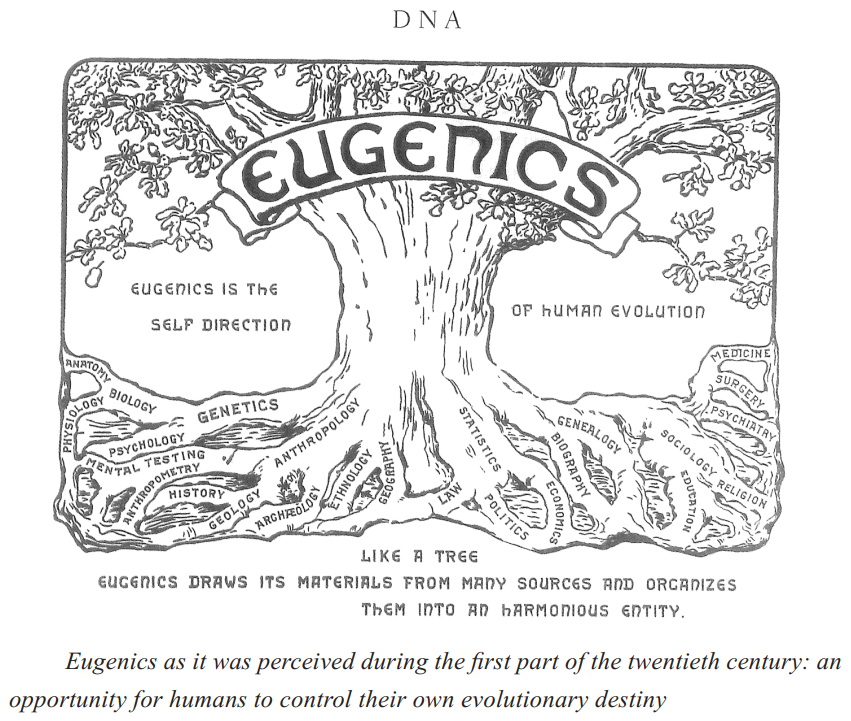
\includegraphics[width=0.75\linewidth]{image/Text5/Fig5.6.png}
\end{figure}

\begin{center}
CHAPTER TWO\\
THE DOUBLE HELIX: THIS IS LIFE\\
双螺旋结构:这就是生命 
\end{center}

\noindent 1\\
I got hooked on the gene during my third year at the University of Chicago. Until then, I had planned to be a naturalist and looked forward to a career far removed from the urban bustle of Chicago’s South Side, where I grew up. My change of heart was inspired not by an unforgettable teacher but a little book that appeared in 1944, *What Is Life?*, by the Austrian-born father of wave mechanics, Erwin Schrödinger. It grew out of several lectures he had given the year before at the Institute for Advanced Study in Dublin. That a great physicist had taken the time to write about biology caught my fancy. In those days, like most people, I considered chemistry and physics to be the “real” sciences, and theoretical physicists were science’s top dogs.\\
我在芝加哥大学读三年级时迷上了基因。在那之前,我原本计划成为一名博物学家,并且期待着从事一份远离我成长的芝加哥南区城市喧嚣的工作。让我改变想法的,不是一位令人难忘的老师,而是1944年出版的一本小书——《生命是什么?》,作者是出生于奥地利的波动力学之父埃尔温·薛定谔。这本书源于他前一年在都柏林高等研究院做的几场讲座。一位伟大的物理学家花时间撰写关于生物学的著作,这引起了我的兴趣。在那个时候,和大多数人一样,我认为化学和物理学才是“真正的”科学,而理论物理学家则是科学界的佼佼者。\\

\noindent 2\\
Schrödinger argued that life could be thought of in terms of storing and passing on biological information. Chromosomes were thus simply information bearers. Because so much information had to be packed into every cell, it must be compressed into what Schrödinger called a “hereditary code-script” embedded in the molecular fabric of chromosomes. To understand life, then, we would have to identify these molecules, and crack their code. He even speculated that understanding life—which would involve finding the gene—might take us beyond the laws of physics as we then understood them. Schrödinger’s book was tremendously influential. Many of those who would become major players in Act 1 of molecular biology’s great drama, including Francis Crick (a former physicist himself), had, like me, read *What Is Life?* and been impressed.\\
薛定谔认为,可以从储存和传递生物信息的角度来理解生命。因此,染色体仅仅是信息的载体。由于每个细胞都要承载大量的信息,这些信息必然被压缩成薛定谔所说的 “遗传密码本”,嵌入染色体的分子结构中。那么,要理解生命,我们就必须识别这些分子,并破解它们的密码。他甚至推测,理解生命——这其中包括找到基因——可能会让我们超越当时对物理定律的认知。薛定谔的这本书极具影响力。许多后来在分子生物学这一伟大篇章的第一幕中扮演重要角色的人,包括弗朗西斯·克里克(他本人曾是一名物理学家),都和我一样读过《生命是什么?》,并深受触动。 \\

\noindent 3\\
In my own case, Schrödinger struck a chord because I too was intrigued by the essence of life. A small minority of scientists still thought life depended upon a vital force emanating from an all - powerful god. But like most of my teachers, I disdained the very idea of vitalism. If such a “vital” force were calling the shots in nature’s game, there was little hope life would ever be understood through the methods of science. On the other hand, the notion that life might be perpetuated by means of an instruction book inscribed in a secret code appealed to me. What sort of molecular code could be so elaborate as to convey all the multitudinous wonder of the living world? And what sort of molecular trick could ensure that the code is exactly copied every time a chromosome duplicates?\\
就我个人而言,薛定谔的观点引起了我的共鸣,因为我也对生命的本质很感兴趣。一小部分科学家仍然认为生命依赖于一种来自全能上帝的生命力。但和我的大多数老师一样,我不屑于生机论这种观点。如果这种 “生命” 力量在主宰着自然界的一切,那么通过科学方法来理解生命就几乎没有希望。另一方面,生命可能通过一种用密码编写的 “说明书” 来延续的观点吸引了我。什么样的分子密码能够如此精妙,足以传达生物世界中所有纷繁复杂的奥秘呢?又是什么样的分子机制能够确保每次染色体复制时,密码都能被精确复制呢? \\

\noindent 4\\
At the time of Schrödinger’s Dublin lectures, most biologists supposed that proteins would eventually be identified as the primary bearers of genetic instruction. Proteins are molecular chains built up from twenty different building blocks, the amino acids. Because permutations in the order of amino acids along the chain are virtually infinite, proteins could, in principle, readily encode the information underpinning life’s extraordinary diversity. DNA then was not considered a serious candidate for the bearer of code-scripts, even though it was exclusively located on chromosomes and had been known about for some seventy-five years. In 1869, Friedrich Miescher, a Swiss biochemist working in Germany, had isolated from pus-soaked bandages supplied by a local hospital a substance he called “nuclein.” Because pus consists largely of white blood cells, which, unlike red blood cells, have nuclei and therefore DNA-containing chromosomes, Miescher had stumbled on a good source of DNA. When he later discovered that “nuclein” was to be found in chromosomes alone, Miescher understood that his discovery was indeed a big one. In 1893, he wrote: “Inheritance insures a continuity in form from generation to generation that lies even deeper than the chemical molecule. It lies in the structuring atomic groups. In this sense, I am a supporter of the chemical heredity theory.”\\
在薛定谔于都柏林举办讲座的时候,大多数生物学家认为,蛋白质最终会被确认为遗传指令的主要载体。蛋白质是由二十种不同的基本组成单位——氨基酸构成的分子链。由于氨基酸在链上的排列顺序几乎是无限的,从理论上来说,蛋白质可以轻松编码构成生命非凡多样性的信息。当时,DNA 并不被视为遗传密码本的有力候选者,尽管它仅存在于染色体上,且人们对它的认知已有七十五年左右。1869 年,在德国工作的瑞士生物化学家弗里德里希·米舍尔,从当地医院提供的沾满脓液的绷带中分离出一种他称之为 “核素” 的物质。因为脓液主要由白细胞组成,与红细胞不同,白细胞有细胞核,因此含有携带 DNA 的染色体,米舍尔偶然间找到了 DNA 的优质来源。后来,当他发现 “核素” 只存在于染色体中时,米舍尔意识到自己的发现意义重大。1893 年,他写道:“遗传确保了代与代之间形式上的连续性,这种连续性比化学分子层面更为深刻。它存在于原子团的结构之中。从这个意义上说,我支持化学遗传理论。” \\

\begin{figure}
    \centering
    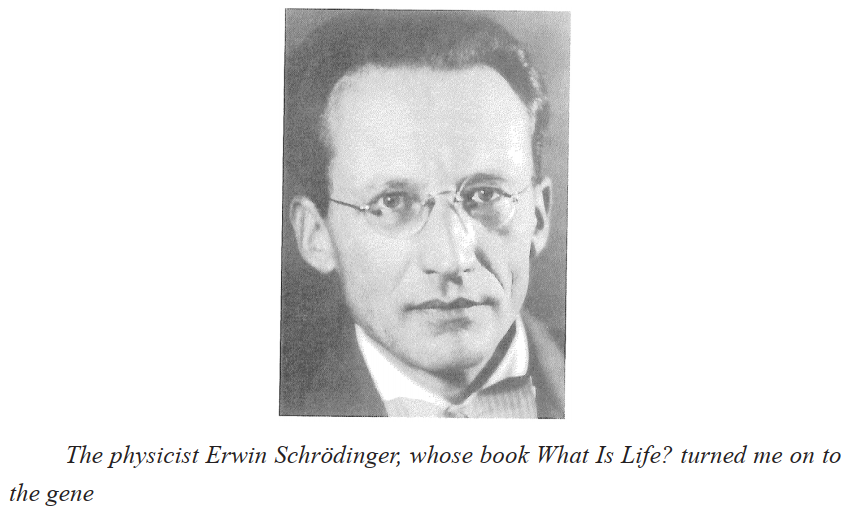
\includegraphics[width=0.75\linewidth]{image/Text5/Fig5.7.png}
\end{figure}

\noindent 5\\
Nevertheless, for decades afterward, chemistry would remain unequal to the task of analyzing the immense size and complexity of the DNA molecule. Only in the 1930s was DNA shown to be a long molecule containing four different chemical bases: adenine (A), guanine (G), thymine (T), and cytosine (C). But at the time of Schrödinger’s lectures, it was still unclear just how the subunits (called deoxynucleotides) of the molecule were chemically linked. Nor was it known whether DNA molecules might vary in their sequences of the four different bases. If DNA were indeed Schrödinger’s code-script, then the molecule would have to be capable of existing in an immense number of different forms. But back then it was still considered a possibility that one simple sequence like AGTC might be repeated over and over along the entire length of DNA chains.\\
然而,在那之后的几十年里,化学在分析 DNA 分子的巨大规模和复杂性方面仍力有不逮。直到20世纪30年代,人们才证明 DNA 是一种长分子,包含四种不同的化学碱基:腺嘌呤(A)、鸟嘌呤(G)、胸腺嘧啶(T)和胞嘧啶(C)。但在薛定谔举办讲座的时候,人们仍不清楚该分子的亚基(称为脱氧核苷酸)是如何通过化学键连接的。人们也不知道 DNA 分子中四种不同碱基的序列是否会有所不同。如果 DNA 确实是薛定谔所说的遗传密码本,那么这种分子必须能够以大量不同的形式存在。但在当时,人们仍认为像 AGTC 这样的简单序列有可能沿着 DNA 链不断重复 。 \\

\noindent 6\\
DNA did not move into the genetic limelight until 1944, when Oswald Avery’s lab at the Rockefeller Institute in New York City reported that the composition of the surface coats of pneumonia bacteria could be changed. This was not the result he and his junior colleagues, Colin MacLeod and Maclyn McCarty, expected.\\
直到1944年,DNA 才成为遗传学领域的焦点。当时,纽约洛克菲勒研究所奥斯瓦尔德·艾弗里的实验室报告称,肺炎细菌的表面荚膜成分可以改变。这并非是他和他的年轻同事科林·麦克劳德以及麦克林恩·麦卡蒂所预期的结果。\\

\noindent 7\\
For more than a decade Avery’s group had been following up on another most unexpected observation made in 1928 by Fred Griffith, a scientist in the British Ministry of Health. Griffith was interested in pneumonia and studied its bacterial agent, *Pneumococcus*. It was known that there were two strains, designated “smooth” (S) and “rough” (R) according to their appearance under the microscope. These strains differed not only visually but also in their virulence. Inject S bacteria into a mouse, and within a few days the mouse dies; inject R bacteria and the mouse remains healthy. It turns out that S bacterial cells have a coating that prevents the mouse’s immune system from recognizing the invader. The R cells have no such coating and are therefore readily attacked by the mouse’s immune defenses.\\
十多年来,艾弗里的研究小组一直在跟进英国卫生部科学家弗雷德·格里菲斯在1928年的一项极其意外的观察发现。格里菲斯对肺炎感兴趣,并研究了引发肺炎的细菌病原体——肺炎球菌。当时已知有两种菌株,根据它们在显微镜下的形态,分别被命名为 “光滑型”(S)和 “粗糙型”(R)。这些菌株不仅在外观上不同,而且在毒力上也有差异。将S型细菌注射到小鼠体内,几天内小鼠就会死亡;注射R型细菌,小鼠则保持健康。事实证明,S型细菌细胞有一层荚膜,可阻止小鼠的免疫系统识别入侵者。而R型细胞没有这种荚膜,因此很容易被小鼠的免疫防御系统攻击。 \\

\begin{figure}
    \centering
    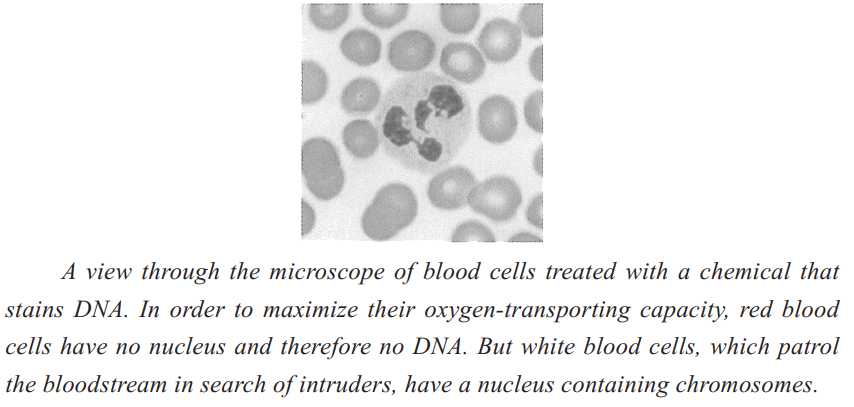
\includegraphics[width=0.75\linewidth]{image/Text5/Fig5.8.png}
\end{figure}

\noindent 8\\
Through his involvement with public health, Griffith knew that multiple strains had sometimes been isolated from a single patient, and so he was curious about how different strains might interact in his unfortunate mice. With one combination, he made a remarkable discovery: when he injected heat-killed S bacteria (harmless) and normal R bacteria (also harmless), the mouse died. How could two harmless forms of bacteria conspire to become lethal? The clue came when he isolated the *Pneumococcus* bacteria retrieved from the dead mice and discovered living S bacteria. It appeared the living innocuous R bacteria had acquired something from the dead S variant; whatever it was, that something had allowed the R in the presence of the heat-killed S bacteria to transform itself into a living killer S strain. Griffith confirmed that this change was for real by culturing the S bacteria from the dead mouse over several generations: the bacteria bred true for the S type, just as any regular S strain would. A genetic change had indeed occurred to the R bacteria injected into the mouse.\\
由于从事公共卫生工作,格里菲斯了解到有时能从单个患者体内分离出多种菌株,因此他很好奇不同的菌株在他用于实验的小鼠体内会如何相互作用。通过一种组合实验,他有了一个惊人的发现:当他将加热杀死的S型细菌(无害)和正常的R型细菌(也无害)注射到小鼠体内时,小鼠死亡了。两种无害的细菌怎么会共同作用而变得致命呢?当他从死亡小鼠体内分离出肺炎球菌,并发现了活的S型细菌时,线索出现了。看起来,活的、无害的R型细菌从死亡的S型细菌变体中获得了某种物质;不管这种物质是什么,它使得R型细菌在加热杀死的S型细菌存在的情况下,转化成了具有致死性的活S型菌株。格里菲斯通过对从死亡小鼠体内获取的S型细菌进行多代培养,证实了这种变化是真实的:这些细菌如同任何正常的S型菌株一样,能够稳定遗传S型的特性。注入小鼠体内的R型细菌确实发生了基因变化。 \\

\noindent 9\\
Though this transformation phenomenon seemed to defy all understanding, Griffith’s observations at first created little stir in the scientific world. This was partly because Griffith was intensely private and so averse to large gatherings that he seldom attended scientific conferences. Once, he had to be virtually forced to give a lecture. Bundled into a taxi and escorted to the hall by colleagues, he discoursed in a mumbled monotone, emphasizing an obscure corner of his microbiological work but making no mention of bacterial transformation. Luckily, however, not everyone overlooked Griffith’s breakthrough.\\
尽管这种转化现象似乎难以理解,但起初,格里菲斯的发现并没有在科学界引起多大轰动。部分原因是格里菲斯极为注重个人隐私,非常反感大型聚会,所以很少参加科学会议。有一次,他几乎是被强迫去做演讲。他被同事塞进出租车,护送到会场,讲话时含糊不清、语调单一,只强调了自己微生物研究中一个不为人知的方面,却对细菌转化只字未提。不过,幸运的是,并非所有人都忽视了格里菲斯的这一突破性发现。 \\

\noindent 10\\
Oswald Avery was also interested in the sugarlike coats of the *Pneumococcus*. He set out to duplicate Griffith’s experiment in order to isolate and characterize whatever it was that had caused those R cells to change to the S type. In 1944 Avery, MacLeod, and McCarty published their results: an exquisite set of experiments showing unequivocally that DNA was the transforming principle. Culturing the bacteria in the test tube rather than in mice made it much easier to search for the chemical identity of the transforming factor in the heat-killed S cells. Methodically destroying one by one the biochemical components of the heat-treated S cells, Avery and his group looked to see whether transformation was prevented. First they degraded the sugarlike coat of the S bacteria. Transformation still occurred: the coat was not the transforming principle. Next they used a mixture of two protein-destroying enzymes, trypsin and chymotrypsin, to degrade virtually all the proteins in the S cells. To their surprise, transformation was again unaffected. Next they tried an enzyme (RNase) that breaks down RNA (ribonucleic acid), a second class of nucleic acids similar to DNA and possibly involved in protein synthesis. Again transformation occurred. Finally, they came to DNA, exposing the S bacterial extracts to the DNA-destroying enzyme, DNase. This time they hit a home run. All S-inducing activity ceased completely. The transforming factor was DNA.\\
奥斯瓦尔德·艾弗里也对肺炎球菌的多糖荚膜感兴趣。他着手重复格里菲思的实验,试图分离并鉴定出使那些R型细胞转变为S型细胞的物质。1944年,艾弗里、麦克劳德和麦卡蒂发表了他们的实验结果:一系列精妙的实验明确表明,DNA就是转化因子。在试管中而非在小鼠体内培养细菌,使得寻找热灭活S型细菌中转化因子的化学本质变得容易得多。艾弗里及其团队有条不紊地逐一破坏热处理后的S型细胞的生化成分,观察转化是否会被阻止。首先,他们降解了S型细菌的多糖荚膜。但转化仍然发生了,这表明荚膜不是转化因子。接下来,他们使用了两种能分解蛋白质的酶(胰蛋白酶和糜蛋白酶)的混合物,几乎降解了S型细胞中的所有蛋白质。令他们惊讶的是,转化再次未受影响。然后,他们尝试使用一种能分解RNA(核糖核酸,一种与DNA类似且可能参与蛋白质合成的核酸)的酶(RNA酶),转化还是发生了。最后,他们研究到了DNA,将S型细菌提取物暴露于能分解DNA的酶(DNA酶)中。这次他们大获成功,所有诱导S型细菌产生的活性完全停止了。由此可知,转化因子就是DNA。\\ 

\noindent 11\\
In part because of its bombshell implications, the resulting February 1944 paper by Avery, MacLeod, and McCarty met with a mixed response. Many geneticists accepted their conclusions. After all, DNA was found on every chromosome; why shouldn’t it be the genetic material? By contrast, however, most biochemists expressed doubt that DNA was a complex enough molecule to act as the repository of such a vast quantity of biological information. They continued to believe that proteins, the other component of chromosomes, would prove to be the hereditary substance. In principle, as the biochemists rightly noted, it would be much easier to encode a vast body of complex information using the twenty - letter amino - acid alphabet of proteins than the four - letter nucleotide alphabet of DNA. Particularly vitriolic in his rejection of DNA as the genetic substance was Avery’s own colleague at the Rockefeller Institute, the protein chemist Alfred Mirsky. By then, however, Avery was no longer scientifically active. The Rockefeller Institute had mandatorily retired him at age sixty - five.\\
部分由于其惊人的意义,艾弗里、麦克劳德和麦卡蒂于1944年2月发表的论文引发了褒贬不一的反响。许多遗传学家接受了他们的结论。毕竟,每条染色体上都有DNA,它为什么不能是遗传物质呢?然而,相比之下,大多数生物化学家对此表示怀疑,他们认为DNA分子的复杂程度不足以成为如此大量生物信息的储存库。他们仍然坚信,染色体的另一种组成成分——蛋白质,才会被证明是遗传物质。从理论上讲,正如生物化学家们正确指出的,用由20种氨基酸组成的 “字母表” 来编码大量复杂信息,要比用由4种核苷酸组成的DNA “字母表” 容易得多。艾弗里在洛克菲勒研究所的同事、蛋白质化学家阿尔弗雷德·米尔施基,对DNA作为遗传物质的观点尤为反感。然而,那时艾弗里已经不再活跃于科研领域,洛克菲勒研究所在他65岁时强制他退休了。\\

\noindent 12\\
Avery missed out on more than the opportunity to defend his work against the attacks of his colleagues: He was never awarded the Nobel Prize, which was certainly his due, for identifying DNA as the transforming principle. Because the Nobel committee makes its records public fifty years following each award, we now know that Avery’s candidacy was blocked by the Swedish physical chemist Einar Hammarsten. Though Hammarsten’s reputation was based largely on his having produced DNA samples of unprecedented high quality, he still believed genes to be an undiscovered class of proteins. In fact, even after the double helix was found, Hammarsten continued to insist that Avery should not receive the prize until after the mechanism of DNA transformation had been completely worked out. Avery died in 1955; had he lived only a few more years, he would almost certainly have gotten the prize.\\
艾弗里错过的不仅仅是为自己的研究成果抵御同事抨击的机会:他因确定DNA是(细菌)转化要素,本应获得诺贝尔奖,却从未获此殊荣。由于诺贝尔奖委员会在每次颁奖五十年后会公布相关记录,我们现在得知,艾弗里的候选人资格被瑞典物理化学家埃纳尔·哈马斯坦否决了。尽管哈马斯坦的声誉主要源于他制备出了前所未有的高质量DNA样本,但他仍然认为基因是一类尚未被发现的蛋白质。事实上,即使在DNA双螺旋结构被发现之后,哈马斯坦仍坚持认为,在DNA转化机制被完全阐明之前,艾弗里不应获奖。艾弗里于1955年去世;要是他能再多活几年,几乎肯定会获得诺贝尔奖。\\

\noindent 13\\
When I arrived at Indiana University in the fall of 1947 with plans to pursue the gene for my Ph.D. thesis, Avery’s paper came up over and over in conversations.
By then, no one doubted the reproducibility of his results, and more recent work coming out of the Rockefeller Institute made it all the less likely that proteins would prove to be the genetic actors in bacterial transformation. DNA had at last become an important objective for chemists setting their sights on the next breakthrough. In Cambridge, England, the canny Scottish chemist Alexander Todd rose to the challenge of identifying the chemical bonds that linked together nucleotides in DNA. By early 1951, his lab had proved that these links were always the same, such that the backbone of the DNA molecule was very regular. During the same period, the Austrian-born refugee Erwin Chargaff, at the College of Physicians and Surgeons of Columbia University, used the new technique of paper chromatography to measure the relative amounts of the four DNA bases in DNA samples extracted from a variety of vertebrates and bacteria. While some species had DNA in which adenine and thymine predominated, others had DNA with more guanine and cytosine. The possibility thus presented itself that no two DNA molecules had the same composition.\\
1947年秋天,我来到印第安纳大学,打算以基因作为博士论文的研究方向,艾弗里的论文在各种讨论中反复被提及。
那时,没人怀疑他的实验结果具有可重复性,而且洛克菲勒研究所最新的研究成果,使蛋白质更不可能被证明是细菌转化中的遗传物质。对于期望取得下一个重大突破的化学家们来说,DNA 最终成为了一个重要的研究目标。在英国剑桥,精明的苏格兰化学家亚历山大·托德接受了挑战,去确定 DNA 中连接核苷酸的化学键。到1951年初,他的实验室已证明这些连接总是相同的,这使得 DNA 分子的骨架非常规则。同一时期,出生于奥地利的难民埃尔文·查格夫,在哥伦比亚大学的内科与外科医师学院,运用纸色谱分析法这一新技术,测量了从多种脊椎动物和细菌中提取的 DNA 样本里四种 DNA 碱基的相对含量。有些物种的 DNA 中腺嘌呤和胸腺嘧啶占主导,而另一些物种的 DNA 中鸟嘌呤和胞嘧啶含量更高。由此可见,没有两个 DNA 分子的组成是相同的,这种可能性是存在的。 \\

\noindent 14\\
At Indiana I joined a small group of visionary scientists, mostly physicists and chemists, studying the reproductive process of the viruses that attack bacteria (bacteriophages—“phages” for short). The Phage Group was born when my Ph.D. supervisor, the Italian-trained medic Salvador Luria and his close friend, the German-born theoretical physicist Max Delbrück, teamed up with the American physical chemist Alfred Hershey. During World War II both Luria and Delbrück were considered enemy aliens, and thus ineligible to serve in the war effort of American science, even though Luria, a Jew, had been forced to leave France for New York City and Delbrück had fled Germany as an objector to Nazism. Thus excluded, they continued to work in their respective university labs—Luria at Indiana and Delbrück at Vanderbilt—and collaborated on phage experiments during successive summers at Cold Spring Harbor. In 1943, they joined forces with the brilliant but taciturn Hershey, then doing phage research of his own at Washington University in St. Louis.\\
在印第安纳大学,我加入了一个由有远见卓识的科学家组成的小团队,成员大多是物理学家和化学家,他们正在研究攻击细菌的病毒(噬菌体,简称 “phages”)的繁殖过程。噬菌体研究小组的成立,源于我的博士导师、在意大利接受医学教育的萨尔瓦多·卢里亚,以及他的挚友、出生于德国的理论物理学家马克斯·德尔布吕克,与美国物理化学家阿尔弗雷德·赫尔希的合作。第二次世界大战期间,卢里亚和德尔布吕克都被视为敌国侨民,因此没有资格参与美国科学界的战时工作,尽管身为犹太人的卢里亚被迫从法国前往纽约,而德尔布吕克作为纳粹主义的反对者逃离了德国。尽管被排除在外,他们仍在各自的大学实验室继续工作——卢里亚在印第安纳大学,德尔布吕克在范德堡大学——并在接下来的几个夏天于冷泉港合作进行噬菌体实验。1943 年,他们与才华横溢但沉默寡言的赫尔希携手合作,当时赫尔希正在圣路易斯的华盛顿大学开展自己的噬菌体研究。 \\

\noindent 15\\
The Phage Group’s program was based on its belief that phages, like all viruses, were in effect naked genes. This concept had first been proposed in 1922 by the imaginative American geneticist Herman J. Muller, who three years later demonstrated that X rays cause mutations. His belated Nobel Prize came in 1946, just after he joined the faculty of Indiana University. It was his presence, in fact, that led me to Indiana. Having started his career under T.H. Morgan, Muller knew better than anyone else how genetics had evolved during the first half of the twentieth century, and I was enthralled by his lectures during my first term. His work on fruit flies (*Drosophila*), however, seemed to me to belong more to the past than to the future, and I only briefly considered doing thesis research under his supervision. I opted instead for Luria’s phages, an even speedier experimental subject than *Drosophila*: genetic crosses of phages done one day could be analyzed the next.\\
噬菌体研究小组的研究计划基于这样一种信念:噬菌体和所有病毒一样,实际上都是裸露的基因。这一概念最早由富有想象力的美国遗传学家赫尔曼·J·穆勒在1922 年提出,三年后,他证明了 X 射线会引发突变。1946 年,在他加入印第安纳大学任教后不久,他终于获得了诺贝尔奖。事实上,正是因为他在那里,我才选择了印第安纳大学。穆勒在托马斯·亨特·摩根手下开始了他的职业生涯,他比任何人都更清楚20世纪上半叶遗传学的发展历程,我在第一学期就被他的讲座深深吸引。然而,在我看来,他关于果蝇(黑腹果蝇)的研究更像是属于过去,而非未来,我只是短暂考虑过在他的指导下进行论文研究。相反,我选择了卢里亚的噬菌体研究,噬菌体是比果蝇更快的实验对象:今天进行的噬菌体杂交实验,明天就可以进行分析。\\

\noindent 16\\
For my Ph.D. thesis research, Luria had me follow in his footsteps by studying how X rays killed phage particles. Initially I had hoped to show that viral death was caused by damage to phage DNA. Reluctantly, however, I eventually had to concede that my experimental approach could never give unambiguous answers at the chemical level. I could draw only biological conclusions. Even though phages were indeed effectively naked genes, I realized that the deep answers the Phage Group was seeking could be arrived at only through advanced chemistry. DNA somehow had to transcend its status as an acronym; it had to be understood as a molecular structure in all its chemical detail.\\
在我的博士论文研究中,卢里亚让我追随他的脚步,研究X射线是如何杀死噬菌体颗粒的。起初,我希望证明病毒的死亡是由噬菌体DNA受损导致的。然而,我最终不得不无奈地承认,我的实验方法永远无法在化学层面给出明确的答案,我只能得出生物学层面的结论。尽管噬菌体实际上确实是裸露的基因,但我意识到,噬菌体研究小组所追寻的深层次答案,只有通过高深的化学知识才能找到。DNA不能仅仅停留在一个缩写词的层面;我们必须从分子结构的所有化学细节上去理解它。\\

\noindent 17\\
Upon finishing my thesis, I saw no alternative but to move to a lab where I could study DNA chemistry. Unfortunately, however, knowing almost no pure chemistry, I would have been out of my depth in any lab attempting difficult experiments in organic or physical chemistry. I therefore took a postdoctoral fellowship in the Copenhagen lab of the biochemist Herman Kalckar in the fall of 1950. He was studying the synthesis of the small molecules that make up DNA, but I figured out quickly that his biochemical approach would never lead to an understanding of the essence of the gene. Every day spent in his lab would be one more day’s delay in learning how DNA carried genetic information.\\
完成博士论文后,我别无选择,只能前往一个能让我研究DNA化学的实验室。然而不幸的是,由于我几乎不懂纯化学知识,在任何试图开展有机化学或物理化学复杂实验的实验室里,我都会力不从心。因此,1950年秋天,我在生物化学家赫尔曼·卡尔卡的哥本哈根实验室获得了一个博士后职位。他当时正在研究构成DNA的小分子的合成,但我很快意识到,他的生物化学研究方法永远无法让我们理解基因的本质。在他的实验室里待的每一天,都会让我在了解DNA如何携带遗传信息这件事上多耽搁一天。\\

\noindent 18\\
My Copenhagen year nonetheless ended productively. To escape the cold Danish spring, I went to the Zoological Station at Naples during April and May. During my last week there, I attended a small conference on X-ray diffraction methods for determining the 3-D structure of molecules. X-ray diffraction is a way of studying the atomic structure of any molecule that can be crystallized. The crystal is bombarded with X rays, which bounce off its atoms and are scattered. The scatter pattern gives information about the structure of the molecule but, taken alone, is not enough to solve the structure. The additional information needed is the “phase assignment,” which deals with the wave properties of the molecule. Solving the phase problem was not easy, and at that time only the most audacious scientists were willing to take it on. Most of the successes of the diffraction method had been achieved with relatively simple molecules.\\
尽管如此,我在哥本哈根的这一年还是颇有收获地结束了。为了躲避丹麦寒冷的春天,我在4月和5月前往那不勒斯的动物研究所。在那里的最后一周,我参加了一个关于利用X射线衍射法测定分子三维结构的小型会议。X射线衍射是一种研究任何可结晶分子原子结构的方法。用X射线轰击晶体,X射线会从晶体的原子上反弹并发生散射。散射图样能提供有关分子结构的信息,但仅靠它不足以确定分子结构。还需要额外的信息,即 “相位确定”,这涉及分子的波动特性。解决相位问题并不容易,当时只有最无畏的科学家才愿意尝试。衍射方法的大多数成功案例都来自相对简单的分子。\\

\noindent 19\\
My expectations for the conference were low. I believed that a three-dimensional understanding of protein structure, or for that matter of DNA, was more than a decade away. Disappointing earlier X-ray photos suggested that DNA was particularly unlikely to yield up its secrets via the X-ray approach. These results were not surprising since the exact sequences of DNA were expected to differ from one individual molecule to another. The resulting irregularity of surface configurations would understandably prevent the long thin DNA chains from lying neatly side by side in the regular repeating patterns required for X-ray analysis to be successful.\\
我对这次会议期望不高。我认为,要从三维层面理解蛋白质结构,或者就此而言理解DNA结构,至少还得等上十多年。早期令人失望的X射线照片表明,DNA尤其不太可能通过X射线分析的方法揭示其奥秘。这些结果并不令人意外,因为不同的DNA分子,其确切序列预计都是不同的。由此产生的表面形态的不规则性,会阻碍细长的DNA链整齐地并排排列成X射线分析所需的规则重复模式,这是可以理解的。\\

\noindent 20\\
It was therefore a surprise and a delight to hear the last-minute talk on DNA by a thirty-four-year-old Englishman named Maurice Wilkins from the Biophysics Lab of King’s College, London. Wilkins was a physicist who during the war had worked on the Manhattan Project. For him, as for many of the other scientists involved, the actual deployment of the bomb on Hiroshima and Nagasaki, supposedly the culmination of all their work, was profoundly disillusioning.\\
因此,当听到来自伦敦国王学院生物物理实验室、34岁的英国科学家莫里斯·威尔金斯在最后一刻做的关于DNA的报告时,我既惊讶又欣喜。威尔金斯是一名物理学家,战时曾参与曼哈顿计划。对他以及许多其他参与该计划的科学家来说,原子弹实际被投放在广岛和长崎,这本应是他们所有工作的顶峰,却让他们深感失望。\\

\begin{figure}
    \centering
    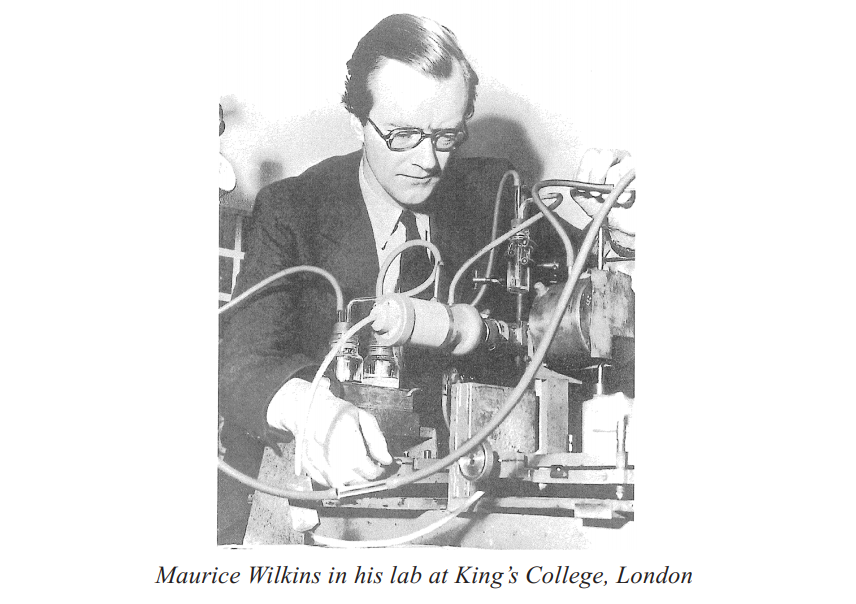
\includegraphics[width=0.75\linewidth]{image/Text5/Fig5.9.png}
\end{figure}

\noindent 21\\
He considered forsaking science altogether to become a painter in Paris, but biology intervened. He too had read Schrödinger’s book, and was now tackling DNA with X-ray diffraction.\\
他曾考虑彻底放弃科学,去巴黎当一名画家,但生物学改变了他的想法。他也读过薛定谔的书,如今正用X射线衍射法研究DNA。\\

\noindent 22\\
He displayed a photograph of an X-ray diffraction pattern he had recently obtained, and its many precise reflections indicated a highly regular crystalline packing. DNA, one had to conclude, must have a regular structure, the elucidation of which might well reveal the nature of the gene. Instantly I saw myself moving to London to help Wilkins find the structure. My attempts to converse with him after his talk, however, went nowhere. All I got for my efforts was a declaration of his conviction that much hard work lay ahead.\\
他展示了一张近期获得的X射线衍射图谱照片,图谱上众多精确的反射图案表明存在高度规则的晶体堆积。由此可以得出结论,DNA必定具有规则的结构,对其结构的阐释很可能会揭示基因的本质。我当即就想着要去伦敦,帮助威尔金斯探寻DNA的结构。然而,他演讲结束后,我试图与他交流,却一无所获。我得到的回应,仅仅是他坚信前路仍有大量艰苦的工作要做。\\

\noindent 23\\
While I was hitting consecutive dead ends, back in America the world’s preeminent chemist, Caltech’s Linus Pauling, announced a major triumph: he had found the exact arrangement in which chains of amino acids (called polypeptides) fold up in proteins, and called his structure the α-helix (alpha helix). That it was Pauling who made this breakthrough was no surprise: he was a scientific superstar. His book *The Nature of the Chemical Bond* essentially laid the foundation of modern chemistry, and, for chemists of the day, it was the Bible. Pauling had been a precocious child. When he was nine, his father, a druggist in Oregon, wrote to the *Oregonian* newspaper requesting suggestions of reading matter for his bookish son, adding that he had already read the Bible and Darwin’s *Origin of Species*. But the early death of Pauling’s father, which brought the family to financial ruin, makes it remarkable that the promising young man managed to get an education at all.\\
在我屡屡碰壁之时,远在美国的世界顶尖化学家、加州理工学院的莱纳斯·鲍林宣布了一项重大成果:他发现了氨基酸链(称为多肽)在蛋白质中折叠的精确方式,并将这种结构称为α-螺旋(阿尔法螺旋)。取得这一突破的是鲍林,这并不令人意外,因为他是科学界的超级巨星。他的著作《化学键的本质》从根本上奠定了现代化学的基础,对于当时的化学家而言,这本书就是 “圣经”。鲍林自幼聪慧过人。九岁时,他在俄勒冈州当药剂师的父亲给《俄勒冈人报》写信,希望为他爱读书的儿子推荐一些读物,还提到他儿子已经读过《圣经》和达尔文的《物种起源》。然而,鲍林父亲的早逝让家庭陷入经济困境,在这种情况下,这位前途无量的年轻人还能接受教育,实在难能可贵。\\

\noindent 24\\
As soon as I returned to Copenhagen I read about Pauling’s α-helix. To my surprise, his model was not based on a deductive leap from experimental X-ray diffraction data. Instead, it was Pauling’s long experience as a structural chemist that had emboldened him to infer which type of helical fold would be most compatible with the underlying chemical features of the polypeptide chain. Pauling made scale models of the different parts of the protein molecule, working out plausible schemes in three dimensions. He had reduced the problem to a kind of three-dimensional jigsaw puzzle in a way that was simple yet brilliant.\\
我一回到哥本哈根,就了解了鲍林的α-螺旋理论。令我惊讶的是,他的模型并非基于从X射线衍射实验数据中得出的推导结论。相反,正是鲍林作为结构化学家的长期经验,让他有底气推断出哪种螺旋折叠方式与多肽链的基本化学特征最为契合。鲍林制作了蛋白质分子不同部分的比例模型,构建出了合理的三维结构方案。他把这个问题简化成了一种三维拼图游戏,方法简单却又十分巧妙。\\

\noindent 25\\
Whether the α-helix was correct—in addition to being pretty—was now the question. Only a week later, I got the answer. Sir Lawrence Bragg, the English inventor of X-ray crystallography and 1915 Nobel laureate in Physics, came to Copenhagen and excitedly reported that his junior colleague, the Austrian-born chemist Max Perutz, had ingeniously used synthetic polypeptides to confirm the correctness of Pauling’s α-helix. It was a bittersweet triumph for Bragg’s Cavendish Laboratory. The year before, they had completely missed the boat in their paper outlining possible helical folds for polypeptide chains.\\
如今的问题是,α-螺旋结构除了看起来精巧之外,是否正确。仅仅一周后,我就得到了答案。英国X射线晶体学的发明者、1915 年诺贝尔物理学奖得主劳伦斯·布拉格爵士来到哥本哈根,兴奋地报告说,他的年轻同事、出生于奥地利的化学家马克斯·佩鲁茨巧妙地利用合成多肽证实了鲍林的α-螺旋结构是正确的。对于布拉格所在的卡文迪许实验室而言,这是一场喜忧参半的胜利。前一年,他们在概述多肽链可能的螺旋折叠方式的论文中完全错失了机会。\\

\begin{figure}
    \centering
    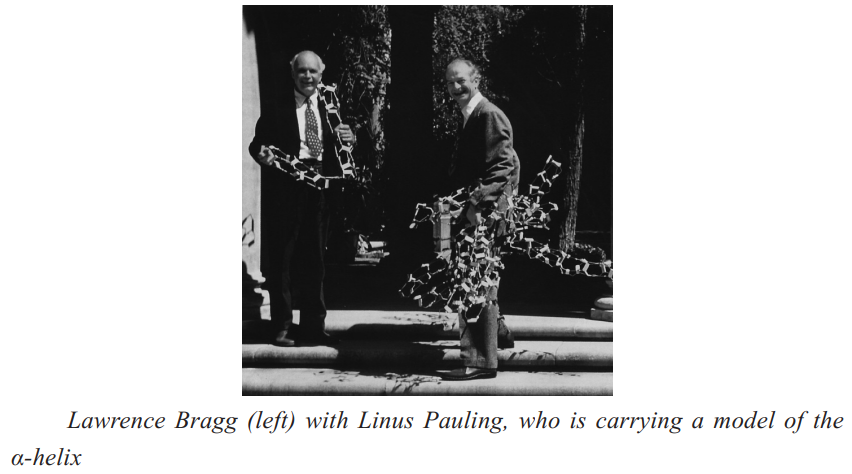
\includegraphics[width=0.75\linewidth]{image/Text5/Fig5.10.png}
\end{figure}

\noindent 26\\
By then Salvador Luria had tentatively arranged for me to take up a research position at the Cavendish. Located at Cambridge University, this was the most famous laboratory in all of science. Here Ernest Rutherford first described the structure of the atom. Now it was Bragg’s own domain, and I was to work as apprentice to the English chemist John Kendrew, who was interested in determining the 3-D structure of the protein myoglobin. Luria advised me to visit the Cavendish as soon as possible. With Kendrew in the States, Max Perutz would check me out. Together, Kendrew and Perutz had earlier established the Medical Research Council (MRC) Unit for the Study of the Structure of Biological Systems.\\
那时,萨尔瓦多·卢里亚已经初步为我安排了在卡文迪许实验室的一个研究职位。该实验室位于剑桥大学,是科学界最负盛名的实验室。欧内斯特·卢瑟福就是在这里首次描述了原子结构。如今这里是布拉格的 “领地”,我将作为英国化学家约翰·肯德鲁的助手开展工作,他致力于确定肌红蛋白的三维结构。卢里亚建议我尽快去卡文迪许实验室看看。由于肯德鲁当时在美国,马克斯·佩鲁茨会对我进行考察。此前,肯德鲁和佩鲁茨共同创立了医学研究委员会(MRC)生物系统结构研究小组。\\

\noindent 27\\
A month later in Cambridge, Perutz assured me that I could quickly master the necessary X-ray diffraction theory and should have no difficulty fitting in with the others in their tiny MRC Unit. To my relief, he was not put off by my biology background. Nor was Lawrence Bragg, who briefly came down from his office to look me over.\\
一个月后,在剑桥,佩鲁茨向我保证,我能很快掌握必要的X射线衍射理论,并且在医学研究委员会这个小研究小组里,与其他人相处也不会有什么困难。令我宽慰的是,他没有因为我的生物学背景而对我有偏见。劳伦斯·布拉格也是如此,他短暂地从办公室下来,对我进行了一番打量。\\

\noindent 28\\
I was twenty-three when I arrived back at the MRC Unit in Cambridge in early October. I found myself sharing space in the biochemistry room with a thirty-five-year-old ex-physicist, Francis Crick, who had spent the war working on magnetic mines for the Admiralty. When the war ended, Crick had planned to stay on in military research, but, on reading Schrödinger’s *What Is Life?*, he had moved toward biology. Now he was at the Cavendish to pursue the 3-D structure of proteins for his Ph.D.\\
10月初,我回到剑桥的医学研究委员会研究小组,那时我23岁。我和一位35岁的前物理学家弗朗西斯·克里克共用生物化学实验室的空间,他在战时曾为英国海军部研究磁性水雷。战争结束后,克里克原本打算继续从事军事研究,但读了薛定谔的《生命是什么?》之后,他转向了生物学领域。如今,他在卡文迪许实验室攻读博士学位,研究蛋白质的三维结构。\\

\noindent 29\\
Crick was always fascinated by the intricacies of important problems. His endless questions as a child compelled his weary parents to buy him a children’s encyclopedia, hoping that it would satisfy his curiosity. But it only made him insecure: he confided to his mother his fear that everything would have been discovered by the time he grew up, leaving him nothing to do. His mother reassured him (correctly, as it happened) that there would still be a thing or two for him to figure out.\\
克里克总是痴迷于重要问题的复杂之处。小时候,他接连不断的提问让疲惫的父母不得不给他买了一本儿童百科全书,希望能满足他的好奇心。但这反而让他感到不安,他向母亲吐露,担心等自己长大后,所有的东西都已被发现,那样他就无事可做了。他母亲安慰他(事实证明这是对的),说总会有一两件事等着他去探索发现。\\

\noindent 30\\
A great talker, Crick was invariably the center of attention in any gathering. His booming laugh was forever echoing down the hallways of the Cavendish. As the MRC Unit’s resident theoretician, he used to come up with a novel insight at least once a month, and he would explain his latest idea at great length to anyone willing to listen. The morning we met he lit up when he learned that my objective in coming to Cambridge was to learn enough crystallography to have a go at the DNA structure. Soon I was asking Crick’s opinion about using Pauling’s model-building approach to go directly for the structure. Would we need many more years of diffraction experimentation before modeling would be practicable? To bring us up to speed on the status of DNA structural studies, Crick invited Maurice Wilkins, a friend since the end of the war, up from London for Sunday lunch. Then we could learn what progress Wilkins had made since his talk in Naples.\\
克里克很健谈,在任何聚会中他总是众人关注的焦点。他爽朗的笑声常常在卡文迪许实验室的走廊里回荡。作为医学研究委员会研究小组的常驻理论家,他过去每个月至少会提出一个新颖的见解,而且会向任何愿意倾听的人详尽地解释他的最新想法。我们见面的那天早上,当他得知我来剑桥的目标是学习足够的晶体学知识,以便研究DNA结构时,他一下子来了兴致。很快,我就向克里克请教关于采用鲍林的模型构建方法直接研究DNA结构的看法。在能够实际构建模型之前,我们还需要进行很多年的衍射实验吗?为了让我们了解DNA结构研究的最新进展,克里克邀请了自二战结束后就相识的朋友莫里斯·威尔金斯从伦敦过来吃周日午餐。这样我们就能知道威尔金斯自从在那不勒斯做报告之后取得了哪些进展。\\

\begin{figure}
    \centering
    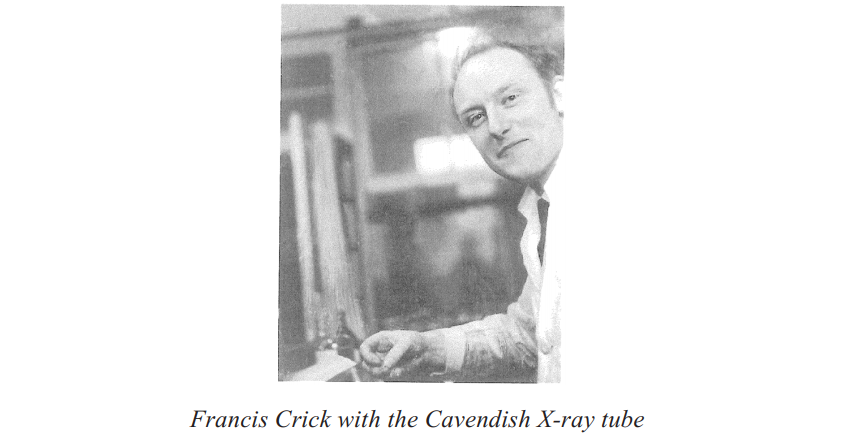
\includegraphics[width=0.75\linewidth]{image/Text5/Fig5.11.png}
\end{figure}

\noindent 31\\
Wilkins expressed his belief that DNA’s structure was a helix, formed by several chains of linked nucleotides twisted around each other. All that remained to be settled was the number of chains. At the time, Wilkins favored three on the basis of his density measurements of DNA fibers. He was keen to start model-building, but he had run into a roadblock in the form of a new addition to the King’s College Biophysics Unit, Rosalind Franklin.\\
威尔金斯表示,他认为DNA的结构是螺旋形,由几条相互缠绕的核苷酸链组成。剩下有待确定的就是链的数量。当时,基于对DNA纤维的密度测量,威尔金斯倾向于三条链的说法。他迫切地想要开始搭建模型,但却遇到了一个阻碍——伦敦国王学院生物物理小组新加入的成员罗莎琳德·富兰克林。\\

\noindent 32\\
A thirty-one-year-old Cambridge-trained physical chemist, Franklin was an obsessively professional scientist; for her twenty-ninth birthday all she requested was her own subscription to her field’s technical journal, *Acta Crystallographica*. Logical and precise, she was impatient with those who acted otherwise. And she was given to strong opinions, once describing her Ph.D. thesis adviser, Ronald Norrish, a future Nobel Laureate, as “stupid, bigoted, deceitful, ill-mannered and tyrannical.” Outside the laboratory, she was a determined and gutsy mountaineer, and, coming from the upper echelons of London society, she belonged to a more rarefied social world than most scientists. At the end of a hard day at the bench, she would occasionally change out of her lab coat into an elegant evening gown and disappear into the night.\\
富兰克林31岁,是一位毕业于剑桥大学的物理化学家,她对科研工作极为执着。29岁生日时,她唯一想要的就是订阅自己所在领域的学术期刊《晶体学报》。她思维逻辑严谨、精确,对行事风格不同的人缺乏耐心。她观点鲜明,曾将自己的博士论文导师、日后的诺贝尔奖得主罗纳德·诺里什描述为 “愚蠢、偏执、虚伪、举止粗俗且专横”。在实验室之外,她是个意志坚定、勇敢无畏的登山爱好者。她出身于伦敦上流社会,所处的社交圈子比大多数科学家更为高雅。在实验室辛苦工作一天后,她偶尔会脱下实验服,换上优雅的晚礼服,消失在夜色中。\\

\begin{figure}
    \centering
    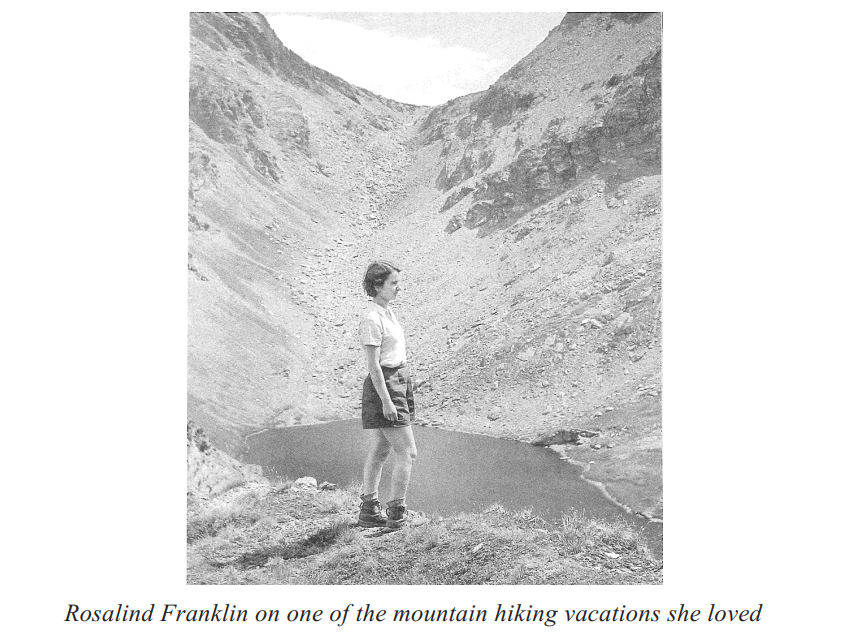
\includegraphics[width=0.75\linewidth]{image/Text5/Fig5.12.png}
\end{figure}

\noindent 33\\
Just back from a four - year X - ray crystallographic investigation of graphite in Paris, Franklin had been assigned to the DNA project while Wilkins was away from King’s. Unfortunately, the pair soon proved incompatible. Franklin, direct and data - focused, and Wilkins, retiring and speculative, were destined never to collaborate. Shortly before Wilkins accepted our lunch invitation, the two had had a big blowup in which Franklin had insisted that no model - building could commence before she collected much more extensive diffraction data. Now they effectively didn’t communicate, and Wilkins would have no chance to learn of her progress until Franklin presented her lab seminar scheduled for the beginning of November. If we wanted to listen, Crick and I were welcome to go as Wilkins’s guests.v
富兰克林刚结束在巴黎为期四年的石墨X射线晶体学研究回到英国,在威尔金斯离开伦敦国王学院期间,她被安排到了DNA研究项目中。不幸的是,两人很快就表现出合不来的情况。富兰克林直率且专注于数据,而威尔金斯内敛又喜欢推测,注定无法合作。就在威尔金斯接受我们的午餐邀请前不久,两人大吵了一架,富兰克林坚持在收集到更广泛的衍射数据之前,不能开始搭建模型。现在他们实际上不再交流,在富兰克林于11月初举办实验室研讨会之前,威尔金斯没有机会了解她的研究进展。如果我和克里克想听研讨会,可以作为威尔金斯的客人一同前往。\\

\noindent 34\\
Crick was unable to make the seminar, so I attended alone and briefed him later on what I believed to be its key take - home messages on crystalline DNA. In particular, I described from memory Franklin’s measurements of the crystallographic repeats and the water content. This prompted Crick to begin sketching helical grids on a sheet of paper, explaining that the new helical X - ray theory he had devised with Bill Cochran and Vladimir Vand would permit even me, a former bird - watcher, to predict correctly the diffraction patterns expected from the molecular models we would soon be building at the Cavendish.\\
克里克没能参加那场研讨会,所以我独自前往,之后我向他简要介绍了我认为这场研讨会中关于结晶DNA的关键要点。我还特别凭记忆描述了富兰克林对晶体学重复间距和含水量的测量结果。这促使克里克开始在纸上绘制螺旋网格,并解释说,他与比尔·科克伦和弗拉基米尔·万德共同提出的螺旋X射线新理论,即使是我这样一个曾经的观鸟爱好者,也能够正确预测我们即将在卡文迪许实验室搭建的分子模型的衍射图样。\\

\noindent 35\\
As soon as we got back to Cambridge, I arranged for the Cavendish machine shop to construct the phosphorous atom models needed for short sections of the sugar phosphate backbone found in DNA. Once these became available, we tested different ways the backbones might twist around each other in the center of the DNA molecule. Their regular repeating atomic structure should allow the atoms to come together in a consistent, repeated conformation. Following Wilkins’s hunch, we focused on three-chain models. When one of these appeared to be almost plausible, Crick made a phone call to Wilkins to announce we had a model we thought might be DNA.\\
我们一回到剑桥,我就安排卡文迪许实验室的机械车间制作DNA中磷酸核糖骨架短链段所需的磷原子模型。模型一做好,我们就测试了这些骨架在DNA分子中心相互缠绕的不同方式。其规则重复的原子结构应能使原子以一致且重复的构象聚集在一起。根据威尔金斯的直觉,我们专注于三链模型。当其中一个模型看起来几乎可行时,克里克打电话给威尔金斯,说我们搭建出了一个认为可能是DNA结构的模型。\\

\noindent 36\\
The next day both Wilkins and Franklin came up to see what we had done. The threat of unanticipated competition briefly united them in common purpose. Franklin wasted no time in faulting our basic concept. My memory was that she had reported almost no water present in crystalline DNA. In fact, the opposite was true. Being a crystallographic novice, I had confused the terms “unit cell” and “asymmetric unit.” Crystalline DNA was in fact water-rich. Consequently, Franklin pointed out, the backbone had to be on the outside and not, as we had it, in the center, if only to accommodate all the water molecules she had observed in her crystals.\\
第二天,威尔金斯和富兰克林都过来看我们的成果。未曾预料到的竞争带来的威胁,让他们在短时间内有了共同目标。富兰克林立刻指出了我们基本构想中的问题。我记得她曾报告说结晶DNA中几乎不含水,而事实恰恰相反。作为晶体学新手,我混淆了 “晶胞” 和 “不对称单位” 这两个术语。实际上,结晶DNA富含水分。因此,富兰克林指出,为了容纳她在晶体中观察到的所有水分子,磷酸 - 脱氧核糖骨架必须位于外侧,而不是像我们所设想的那样位于中心。\\

\noindent 37\\
That unfortunate November day cast a very long shadow. Franklin’s opposition to model-building was reinforced. Doing experiments, not playing with Tinkertoy representations of atoms, was the way she intended to proceed. Even worse, Sir Lawrence Bragg passed down the word that Crick and I should desist from all further attempts at building a DNA model. It was further decreed that DNA research should be left to the King’s lab, with Cambridge continuing to focus solely on proteins. There was no sense in two MRC-funded labs competing against each other. With no more bright ideas up our sleeves, Crick and I were reluctantly forced to back off, at least for the time being.\\
那个不幸的11月的日子带来了长久的影响。富兰克林更加反对搭建模型了。她打算通过做实验,而不是摆弄原子模型来开展研究。更糟糕的是,劳伦斯·布拉格爵士传话下来,让我和克里克停止一切进一步搭建DNA模型的尝试。他还下令DNA研究应该由伦敦国王学院的实验室负责,剑桥这边继续只专注于蛋白质研究。两个由医学研究委员会资助的实验室相互竞争毫无意义。由于我们也没有新的好主意,我和克里克只好不情愿地暂时放弃。\\

\noindent 38\\
It was not a good moment to be condemned to the DNA sidelines. Linus Pauling had written Wilkins to request a copy of the crystalline DNA diffraction pattern. Though Wilkins had declined, saying he wanted more time to interpret it himself, Pauling was hardly obliged to depend upon data from King’s. If he wished, he could easily start serious X-ray diffraction studies at Caltech.\\
被排除在DNA研究之外可不是个好时候。莱纳斯·鲍林写信给威尔金斯,索要一份结晶DNA的衍射图谱。尽管威尔金斯拒绝了,称自己还需要更多时间来分析图谱,但鲍林并非只能依靠国王学院的数据。如果他愿意,他可以很容易地在加州理工学院开展严谨的X射线衍射研究。\\

\noindent 39\\
The following spring, I duly turned away from DNA and set about extending prewar studies on the pencil-shaped tobacco mosaic virus using the Cavendish’s powerful new X-ray beam. This light experimental workload gave me plenty of time to wander through various Cambridge libraries. In the zoology building, I read Erwin Chargaff’s paper describing his finding that the DNA bases adenine and thymine occurred in roughly equal amounts, as did the bases guanine and cytosine. Hearing of these one-to-one ratios Crick wondered whether, during DNA duplication, adenine residues might be attracted to thymine and vice versa, and whether a corresponding attraction might exist between guanine and cytosine. If so, base sequences on the “parental” chains (e.g., ATGC) would have to be complementary to those on “daughter” strands (yielding in this case TACG). \\
第二年春天,我顺从地放下了DNA研究,开始利用卡文迪许实验室强大的新型X射线束,拓展对铅笔状烟草花叶病毒的战前研究。实验任务不重,这让我有大量时间流连于剑桥的各个图书馆。在动物学楼里,我读到了埃尔文·查戈夫的论文,他在文中描述了自己的发现:DNA中的腺嘌呤和胸腺嘧啶的含量大致相等,鸟嘌呤和胞嘧啶的含量也是如此。听到这些碱基一一对应的比例关系后,克里克猜想,在DNA复制过程中,腺嘌呤残基是否会被胸腺嘧啶吸引,反之亦然,以及鸟嘌呤和胞嘧啶之间是否也存在类似的吸引关系。如果是这样, “亲代” 链上的碱基序列(例如ATGC)就必须与 “子代” 链上的互补(在这种情况下是TACG)。\\ 

\noindent 40\\
These remained idle thoughts until Erwin Chargaff came through Cambridge in the summer of 1952 on his way to the International Biochemical Congress in Paris. Chargaff expressed annoyance that neither Crick nor I saw the need to know the chemical structures of the four bases. He was even more upset when we told him that we could simply look up the structures in textbooks as the need arose. I was left hoping that Chargaff’s data would prove irrelevant. Crick, however, was energized to do several experiments looking for molecular “sandwiches” that might form when adenine and thymine (or alternatively, guanine and cytosine) were mixed together in solution. But his experiments went nowhere.\\
这些想法一直停留在空想阶段,直到1952年夏天埃尔文·查戈夫途经剑桥前往巴黎参加国际生物化学大会。查戈夫很恼火,因为我和克里克都觉得没必要了解四种碱基的化学结构。当我们告诉他,有需要时我们可以直接在教科书里查阅这些结构时,他更生气了。我暗自希望查戈夫的数据被证明是无关紧要的。然而,克里克却充满干劲地做了几个实验,试图找出腺嘌呤和胸腺嘧啶(或者鸟嘌呤和胞嘧啶)在溶液中混合时可能形成的分子 “夹层” 结构,但他的实验毫无进展。 \\

\noindent 41\\
Like Chargaff, Linus Pauling also attended the International Biochemical Congress, where the big news was the latest result from the Phage Group. Alfred Hershey and Martha Chase at Cold Spring Harbor had just confirmed Avery’s transforming principle: DNA was the hereditary material! Hershey and Chase proved that only the DNA of the phage virus enters bacterial cells; its protein coat remains on the outside. It was more obvious than ever that DNA must be understood at the molecular level if we were to uncover the essence of the gene. With Hershey and Chase’s result the talk of the town, I was sure that Pauling would now bring his formidable intellect and chemical wisdom to bear on the problem of DNA.\\
和查戈夫一样,莱纳斯·鲍林也参加了国际生物化学大会,大会上的重大新闻是噬菌体小组的最新研究成果。冷泉港实验室的阿尔弗雷德·赫尔希和玛莎·蔡斯刚刚证实了艾弗里的转化原理:DNA是遗传物质!赫尔希和蔡斯证明,只有噬菌体病毒的DNA会进入细菌细胞,其蛋白质外壳则留在细胞外。现在比以往任何时候都更明显的是,如果我们想要揭示基因的本质,就必须从分子层面去理解DNA。赫尔希和蔡斯的研究成果成了人们热议的话题,我确信鲍林现在会运用他卓越的智慧和化学知识来研究DNA问题。\\

\noindent 42\\
Early in 1953, Pauling did indeed publish a paper outlining the structure of DNA. Reading it anxiously I saw that he was proposing a three-chain model with sugar phosphate backbones forming a dense central core. Superficially it was similar to our botched model of fifteen months earlier. But instead of using positively charged atoms (e.g., Mg²⁺) to stabilize the negatively charged backbones, Pauling made the unorthodox suggestion that the phosphates were held together by hydrogen bonds. But it seemed to me, the biologist, that such hydrogen bonds required extremely acidic conditions never found in cells. With a mad dash to Alexander Todd’s nearby organic chemistry lab my belief was confirmed: The impossible had happened. The world’s best-known, if not best, chemist had gotten his chemistry wrong. In effect, Pauling had knocked the A off of DNA. Our quarry was deoxyribonucleic acid, but the structure he was proposing was not even acidic.\\
1953年初,鲍林确实发表了一篇概述DNA结构的论文。我急切地读完后发现,他提出了一个三链模型,其中磷酸核糖骨架形成一个致密的核心。从表面上看,这与我们15个月前失败的模型相似。但鲍林没有使用带正电的原子(如镁离子Mg²⁺)来稳定带负电的骨架,而是提出了一个非传统的观点,即磷酸盐是通过氢键结合在一起的。但在我这个生物学家看来,这种氢键的形成需要细胞中不存在的强酸性条件。我急忙跑到附近亚历山大·托德的有机化学实验室,证实了我的想法:不可能的事情发生了。这位世界上最知名(即便不是最优秀)的化学家在化学问题上出错了。实际上,鲍林颠覆了DNA中的 “酸(acid)” 这一概念。我们要研究的是脱氧核糖核酸,但他提出的结构甚至都不具备酸性。\\

\noindent 43\\
Hurriedly I took the manuscript to London to inform Wilkins and Franklin they were still in the game. Convinced that DNA was not a helix, Franklin had no wish even to read the article and deal with the distraction of Pauling’s helical ideas, even when I offered Crick’s arguments for helices. Wilkins, however, was very interested indeed in the news I brought; he was now more certain than ever that DNA was helical. To prove the point, he showed me a photograph obtained more than six months earlier by Franklin’s graduate student Raymond Gosling, who had X-rayed the so-called B form of DNA. Until that moment, I didn’t know a B form even existed. Franklin had put this picture aside, preferring to concentrate on the A form, which she thought would more likely yield useful data. The X-ray pattern of this B form was a distinct cross. Since Crick and others had already deduced that such a pattern of reflections would be created by a helix, this evidence made it clear that DNA had to be a helix! In fact, despite Franklin’s reservations, this was no surprise. Geometry itself suggested that a helix was the most logical arrangement for a long string of repeating units such as the nucleotides of DNA. But we still did not know what that helix looked like, nor how many chains it contained.\\
我匆忙带着这份手稿前往伦敦,告诉威尔金斯和富兰克林,他们仍有机会在DNA结构研究上取得成果。富兰克林坚信DNA不是螺旋结构,甚至不愿去读鲍林的那篇文章,也不想理会鲍林有关螺旋结构的观点,即便我提出了克里克支持螺旋结构的论据。然而,威尔金斯对我带来的消息非常感兴趣,他比以往任何时候都更加确信DNA是螺旋形的。为了证明这一点,他给我看了一张照片,那是富兰克林的研究生雷蒙德·戈斯林在六个多月前拍摄的,是对所谓的B型DNA进行X射线衍射的结果。在那之前,我甚至都不知道还有B型DNA的存在。富兰克林把这张照片搁置了,她更倾向于专注研究A型DNA,认为其更有可能产生有用的数据。B型DNA的X射线衍射图谱呈现出一个清晰的十字形。由于克里克和其他人此前已经推断出,这样的衍射图谱是由螺旋结构产生的,所以这一证据清楚地表明,DNA必定是螺旋结构!事实上,尽管富兰克林持保留意见,但这并不意外。从几何学角度来看,对于像DNA中的核苷酸这样一长串重复单元而言,螺旋结构是最合理的排列方式。但我们仍然不知道这个螺旋结构是什么样子,也不清楚它包含多少条链。\\ 

\noindent 44\\
The time had come to resume building helical models of DNA. Pauling was bound to realize soon enough that his brainchild was wrong. I urged Wilkins to waste no time. But he wanted to wait until Franklin had completed her scheduled departure for another lab later that spring. She had decided to move on to avoid the unpleasantness at King’s. Before leaving, she had been ordered to stop further work with DNA and had already passed on many of her diffraction images to Wilkins.\\
是时候重新开始搭建DNA的螺旋结构模型了。鲍林很快就会意识到,他的心血之作是错误的。我催促威尔金斯不要浪费时间。但他想等到富兰克林在那年春天晚些时候按计划离开,前往另一个实验室之后再说。她为了避免在伦敦国王学院的不愉快而决定离开。在离开之前,她被要求停止DNA相关的进一步研究工作,并且已经把自己的许多衍射图像交给了威尔金斯。\\

\begin{figure}
    \centering
    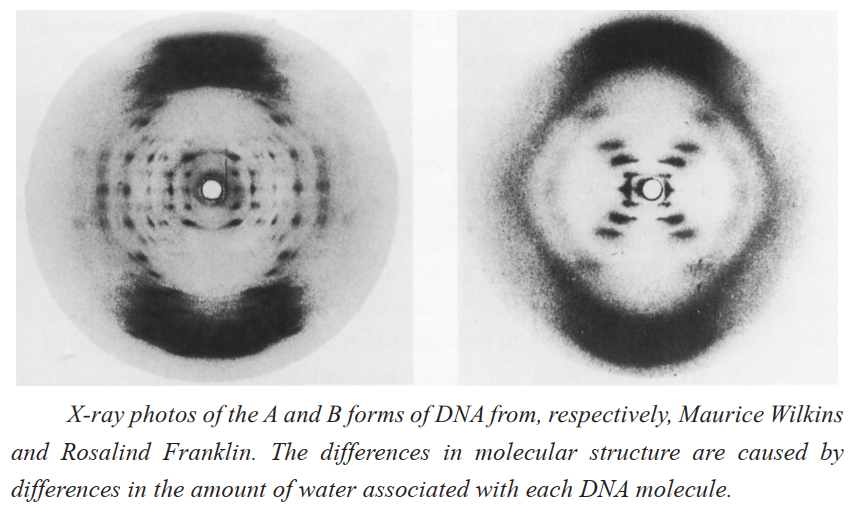
\includegraphics[width=0.75\linewidth]{image/Text5/Fig5.13.png}
\end{figure}

\noindent 45\\
When I returned to Cambridge and broke the news of the DNA B form, Bragg no longer saw any reason for Crick and me to avoid DNA. He very much wanted the DNA structure to be found on his side of the Atlantic. So we went back to model - building, looking for a way the known basic components of DNA—the backbone of the molecule and the four different bases, adenine, thymine, guanine, and cytosine—could fit together to make a helix. I commissioned the shop at the Cavendish to make us a set of tin bases, but they couldn’t produce them fast enough for me: I ended up cutting out rough approximations from stiff cardboard.\\
我回到剑桥,把发现DNA B型结构的消息告知大家后,布拉格认为我和克里克没有理由再避开DNA研究了。他非常希望能由大西洋这边(即英国)的团队发现DNA的结构。于是我们重新开始搭建模型,试图找到一种方式,将已知的DNA基本组成部分——分子骨架以及腺嘌呤、胸腺嘧啶、鸟嘌呤和胞嘧啶这四种不同的碱基——组合在一起,形成螺旋结构。我请卡文迪许实验室的车间制作一套金属碱基模型,但他们的制作速度无法满足我的需求,最后我只好用硬纸板剪出大致的模型。\\

\noindent 46\\
By this time I realized the DNA density-measurement evidence actually slightly favored a two-chain, rather than three-chain, model. So I decided to search out plausible double helices. As a biologist, I preferred the idea of a genetic molecule made of two, rather than three, components. After all, chromosomes, like cells, increase in number by duplicating, not triplicating.
这时我意识到,DNA密度测量的证据实际上更倾向于双链模型,而非三链模型。所以我决定寻找合理的双螺旋结构。作为一名生物学家,我更倾向于遗传分子由两部分组成,而不是三部分。毕竟,染色体和细胞一样,是通过复制(加倍)而非 “复制三倍” 来增加数量的。\\

\begin{figure}
    \centering
    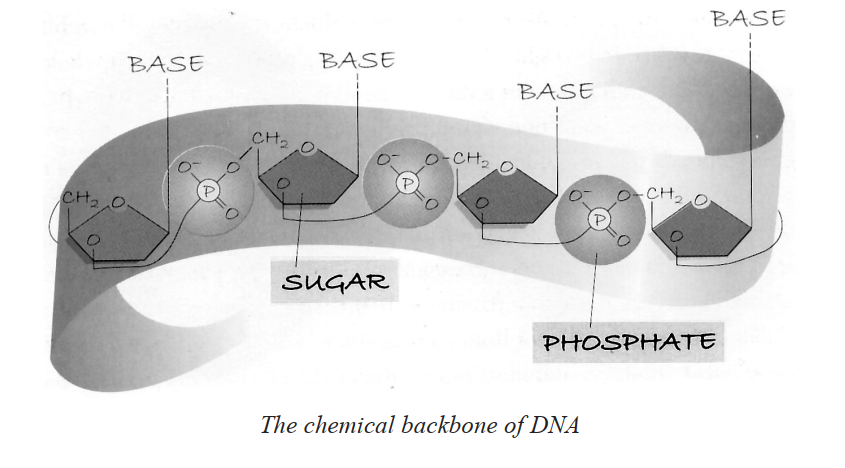
\includegraphics[width=0.75\linewidth]{image/Text5/Fig5.14.png}
\end{figure}

\noindent 47\\
I knew that our previous model with the backbone on the inside and the bases hanging out was wrong. Chemical evidence from the University of Nottingham, which I had too long ignored, indicated that the bases must be hydrogen-bonded to each other. They could only form bonds like this in the regular manner implied by the X-ray diffraction data if they were in the center of the molecule. But how could they come together in pairs? For two weeks I got nowhere, misled by an error in my nucleic acid chemistry textbook. Happily, on February 27, Jerry Donahue, a theoretical chemist visiting the Cavendish from Caltech, pointed out that the textbook was wrong. So I changed the locations of the hydrogen atoms on my cardboard cutouts of the molecules.\\
我知道,我们之前提出的磷酸 - 脱氧核糖骨架在内、碱基在外的模型是错误的。诺丁汉大学的化学研究证据表明,碱基之间必定存在氢键,而我此前一直忽视了这一点。根据X射线衍射数据显示,如果碱基位于分子中心,它们才能以规律的方式形成这样的化学键。但它们如何成对结合呢?有两周时间,我毫无进展,被核酸化学教科书里的一个错误误导了。幸运的是,2月27日,从加州理工学院到卡文迪许实验室访问的理论化学家杰里·多纳休指出了教科书里的错误。于是我更改了用硬纸板剪出的分子模型上氢原子的位置。 \\

\noindent 48\\
The next morning, February 28, 1953, the key features of the DNA model all fell into place. The two chains were held together by strong hydrogen bonds between adenine-thymine and guanine-cytosine base pairs. The inferences Crick had drawn the year before based on Chargaff’s research had indeed been correct. Adenine does bond to thymine and guanine does bond to cytosine, but not through flat surfaces to form molecular sandwiches. When Crick arrived, he took it all in rapidly, and gave my base-pairing scheme his blessing. He realized right away that it would result in the two strands of the double helix running in opposite directions.\\
第二天早上,也就是1953年2月28日,DNA模型的关键特征都确定下来了。两条链通过腺嘌呤 - 胸腺嘧啶以及鸟嘌呤 - 胞嘧啶碱基对之间的强氢键结合在一起。克里克前一年基于查戈夫的研究所得出的推论确实是正确的。腺嘌呤与胸腺嘧啶结合,鸟嘌呤与胞嘧啶结合,但不是通过平面形成分子 “夹层” 结构。克里克到了之后,很快理解了整个模型,并认可了我的碱基配对方案。他立刻意识到,这会使得双螺旋的两条链方向相反。 \\

\noindent 49\\
It was quite a moment. We felt sure that this was it. Anything that simple, that elegant just had to be right. What got us most excited was the complementarity of the base sequences along the two chains. If you knew the sequence—the order of bases—along one chain, you automatically knew the sequence along the other. It was immediately apparent that this must be how the genetic messages of genes are copied so exactly when chromosomes duplicate prior to cell division. The molecule would “unzip” to form two separate strands. Each separate strand then could serve as the template for the synthesis of a new strand, one double helix becoming two.\\
那真是一个激动人心的时刻。我们确信就是它了。如此简单而又精妙的结构,必定是正确的。最让我们兴奋的是两条链上碱基序列的互补性。如果你知道一条链上的碱基序列,就能自然而然地知道另一条链上的序列。很明显,这一定就是在细胞分裂前染色体复制时,基因的遗传信息能够精确复制的方式。DNA分子会 “解旋” 形成两条单链,随后每条单链都可以作为合成新链的模板,一个双螺旋结构就变成了两个。 \\

\noindent 50\\
In *What is Life?* Schrödinger had suggested that the language of life might be like Morse code, a series of dots and dashes. He wasn’t far off. The language of DNA is a linear series of As, Ts, Gs, and Cs. And just as transcribing a page out of a book can result in the odd typo, the rare mistake creeps in when all these As, Ts, Gs, and Cs are being copied along a chromosome. These errors are the mutations geneticists had talked about for almost fifty years. Change an “i” to an “a” and “Jim” becomes “Jam” in English; change a T to a C and “ATG” becomes “ACG” in DNA.\\
在《生命是什么?》一书中,薛定谔曾提出,生命的语言可能就像摩尔斯电码,由一系列的点和划组成。他的想法相差不远。DNA的 “语言” 是由腺嘌呤(A)、胸腺嘧啶(T)、鸟嘌呤(G)和胞嘧啶(C)组成的线性序列。就像抄写书中的一页内容可能会出现偶尔的拼写错误一样,当这些A、T、G和C在染色体中被复制时,也会偶尔出现罕见的错误。这些错误就是遗传学家们近五十年来一直在讨论的突变。在英语中,把 “i” 改成 “a”,“Jim” 就变成了 “Jam” ;在DNA中,把T改成C,“ATG” 就变成了 “ACG”。 \\

\begin{figure}
    \centering
    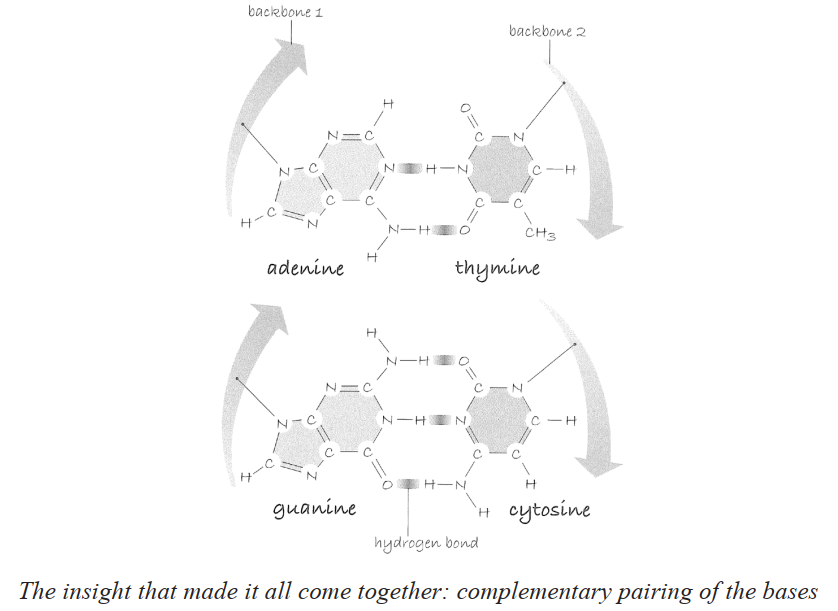
\includegraphics[width=0.75\linewidth]{image/Text5/Fig5.15.png}
\end{figure}

\begin{figure}
    \centering
    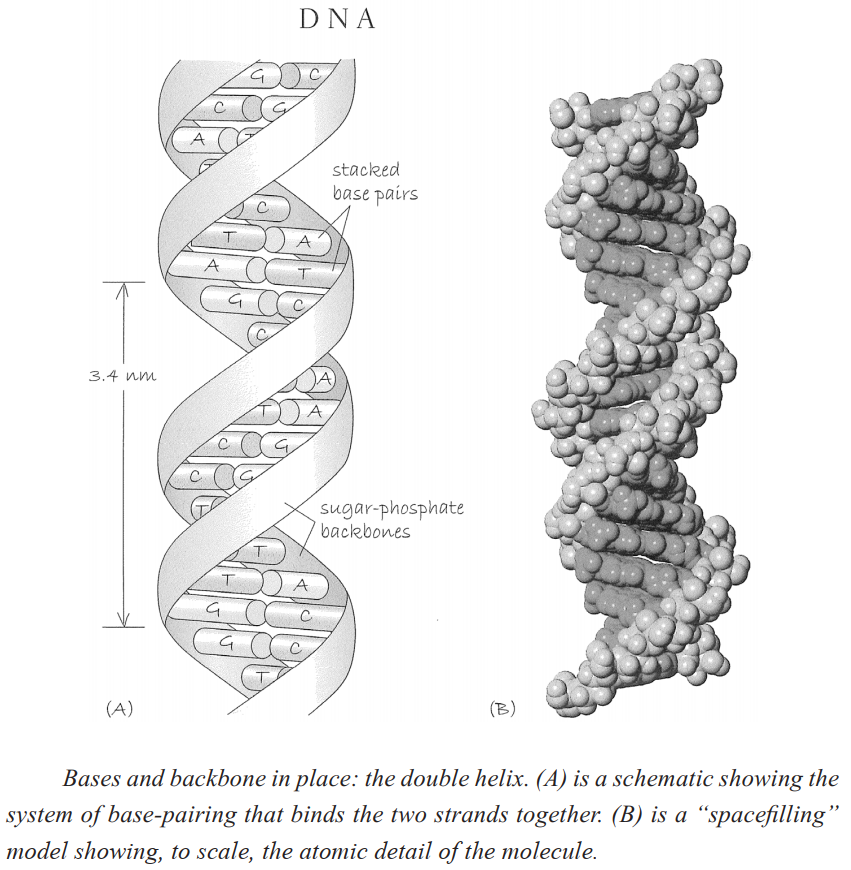
\includegraphics[width=0.75\linewidth]{image/Text5/Fig5.16.png}
\end{figure}

\noindent 51\\
The double helix made sense chemically and it made sense biologically. Now there was no need to be concerned about Schrödinger’s suggestion that new laws of physics might be necessary for an understanding of how the hereditary code-script is duplicated: genes in fact were no different from the rest of chemistry. Later that day, during lunch at the Eagle, the pub virtually adjacent to the Cavendish Lab, Crick, ever the talker, could not help but tell everyone we had just found the “secret of life.” I myself, though no less electrified by the thought, would have waited until we had a pretty three-dimensional model to show off.\\
DNA双螺旋结构在化学和生物学上都有其合理性。现在,也无需担心薛定谔曾提出的观点,即可能需要新的物理定律来解释遗传密码是如何复制的:事实上,基因与其他化学物质并无不同。那天晚些时候,在卡文迪许实验室附近的老鹰酒吧吃午饭时,一向健谈的克里克忍不住告诉每个人,我们刚刚发现了 “生命的奥秘” 。而我自己,虽然同样为此兴奋不已,但本想等到做出一个精美的三维模型后再炫耀。 \\

\noindent 52\\
Among the first to see our demonstration model was the chemist Alexander Todd. That the nature of the gene was so simple both surprised and pleased him. Later, however, he must have asked himself why his own lab, having established the general chemical structure of DNA chains, had not moved on to asking how the chains folded up in three dimensions. Instead the essence of the molecule was left to be discovered by a two - man team, a biologist and a physicist, neither of whom possessed a detailed command even of undergraduate chemistry. But paradoxically, this was, at least in part, the key to our success: Crick and I arrived at the double helix first precisely because most chemists at that time thought DNA too big a molecule to understand by chemical analysis.\\
最早看到我们演示模型的人之一是化学家亚历山大·托德。基因的本质如此简单,这既让他感到惊讶,又让他欣喜。然而,后来他肯定反思过,为什么自己的实验室在确定了DNA链的一般化学结构后,却没有进一步研究这些链是如何折叠成三维结构的。最终,这个分子的奥秘却是由一个两人团队发现的,团队成员一个是生物学家,一个是物理学家,他们甚至都没有全面掌握本科化学知识。但矛盾的是,这至少在一定程度上是我们成功的关键:我和克里克之所以能率先发现双螺旋结构,恰恰是因为当时大多数化学家都认为DNA分子太大,无法通过化学分析来理解 。 \\

\noindent 53\\
At the same time, the only two chemists with the vision to seek DNA’s 3-D structure made major tactical mistakes: Rosalind Franklin’s was her resistance to model-building; Linus Pauling’s was a matter of simply neglecting to read the existing literature on DNA, particularly the data on its base composition published by Chargaff. Ironically, Pauling and Chargaff sailed across the Atlantic on the same ship following the Paris Biochemical Congress in 1952, but failed to hit it off. Pauling was long accustomed to being right. And he believed there was no chemical problem he could not work out from first principles by himself. Usually this confidence was not misplaced. During the Cold War, as a prominent critic of the American nuclear weapons development program, he was questioned by the FBI after giving a talk. How did he know how much plutonium there is in an atomic bomb? Pauling’s response was “Nobody told me. I figured it out.”\\
与此同时,仅有的两位有远见去探寻DNA三维结构的化学家都犯了重大的策略性错误:罗莎琳德·富兰克林的错误在于她抵触搭建模型;莱纳斯·鲍林的问题则是完全忽视了阅读现有的关于DNA的文献,特别是查戈夫发表的有关DNA碱基组成的数据。具有讽刺意味的是,1952年巴黎生物化学大会之后,鲍林和查戈夫同船穿越大西洋,但两人却没能谈得来。鲍林长期以来习惯了自己总是正确的。他相信没有什么化学问题是他不能从基本原理出发独自解决的。通常情况下,这种自信并非毫无根据。冷战期间,作为美国核武器发展计划的著名批评者,他在一次演讲后被美国联邦调查局讯问。他们问他是怎么知道一颗原子弹里有多少钚的,鲍林回答说:“没人告诉我,我自己算出来的。” \\

\noindent 54\\
Over the next several months Crick and (to a lesser extent) I relished showing off our model to an endless stream of curious scientists. However, the Cambridge biochemists did not invite us to give a formal talk in the biochemistry building. They started to refer to it as the “WC,” punning our initials with those used in Britain for the toilet or water closet. That we had found the double helix without doing experiments irked them.\\
在接下来的几个月里,克里克以及我(相对少一些)乐于向源源不断的好奇科学家展示我们的模型。然而,剑桥的生物化学家们没有邀请我们在生物化学楼里进行正式演讲。他们开始戏称这个模型为 “WC”,这是拿我们姓氏的首字母和英国表示厕所的缩写玩双关。我们没做实验就发现了双螺旋结构,这让他们很恼火。\ 

\noindent 55\\
The manuscript that we submitted to *Nature* in early April was published just over three weeks later, on April 25, 1953. Accompanying it were two longer papers by Franklin and Wilkins, both supporting the general correctness of our model. In June, I gave the first presentation of our model at the Cold Spring Harbor symposium on viruses. Max Delbrück saw to it that I was offered, at the last minute, an invitation to speak. To this intellectually high-powered meeting I brought a three-dimensional model built in the Cavendish, the adenine-thymine base pairs in red and the guanine-cytosine base pairs in green.\\
我们在4月初提交给《自然》杂志的论文,在三周多一点后的1953年4月25日发表了。一同发表的还有富兰克林和威尔金斯的两篇篇幅更长的论文,他们都认可我们提出的DNA模型在总体上是正确的。6月,我在冷泉港病毒研讨会上首次介绍了我们的模型。马克斯·德尔布吕克安排我在最后一刻得到了发言邀请。在这场学术大咖云集的会议上,我展示了一个在卡文迪许实验室制作的三维模型,其中腺嘌呤 - 胸腺嘧啶碱基对是红色的,鸟嘌呤 - 胞嘧啶碱基对是绿色的。 \\

\begin{figure}
    \centering
    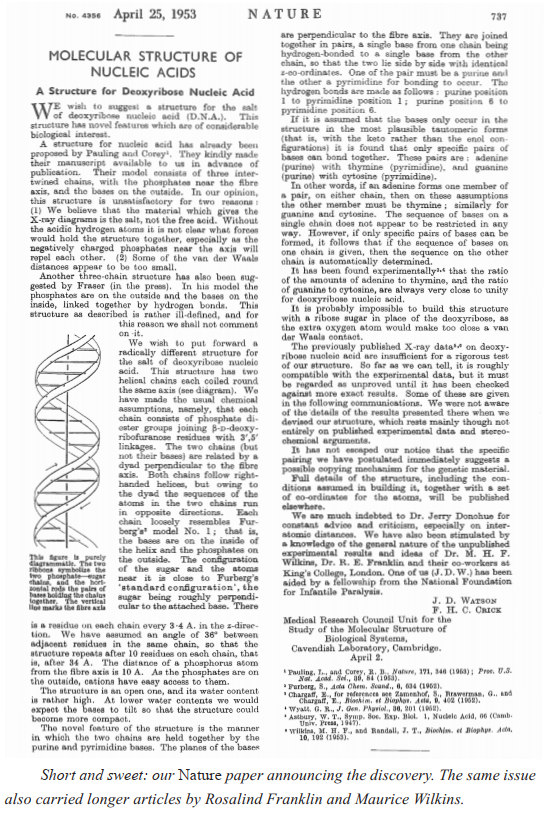
\includegraphics[width=0.75\linewidth]{image/Text5/Fig5.17.png}
\end{figure}

\begin{figure}
    \centering
    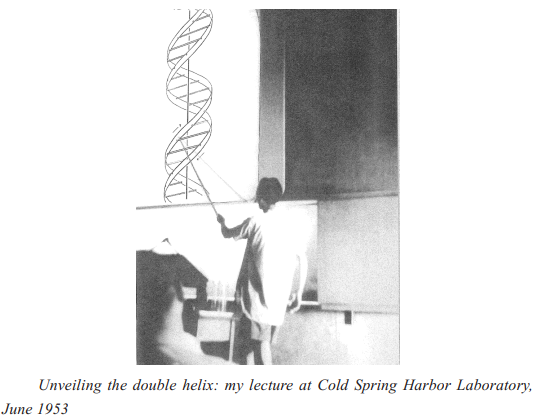
\includegraphics[width=0.75\linewidth]{image/Text5/Fig5.18.png}
\end{figure}

\noindent 56\\
In the audience was Seymour Benzer, yet another ex - physicist who had heeded the clarion call of Schrödinger’s book. He immediately understood what our breakthrough meant for his studies of mutations in viruses. He realized that he could now do for a short stretch of bacteriophage DNA what Morgan’s boys had done forty years earlier for fruit fly chromosomes: he would map mutations—determine their order—along a gene, just as the fruit fly pioneers had mapped genes along a chromosome. Like Morgan, Benzer would have to depend on recombination to generate new genetic combinations, but, whereas Morgan had the advantage of a ready mechanism of recombination—the production of sex cells in a fruit fly—Benzer had to induce recombination by simultaneously infecting a single bacterial host cell with two different strains of bacteriophage, which differed by one or more mutations in the region of interest. Within the bacterial cell, recombination—the exchange of segments of molecules—would occasionally occur between the different viral DNA molecules, producing new permutations of mutations—so - called “recombinants.” Within a single astonishingly productive year in his Purdue University lab, Benzer produced a map of a single bacteriophage gene, *rII*, showing how a series of mutations—all errors in the genetic script—were laid out linearly along the virus DNA. The language was simple and linear, just like a line of text on the written page.\\
听众中有西摩·本泽,他也是一位从前的物理学家,曾响应薛定谔著作的号召转行。他立刻明白我们的突破对他研究病毒突变意味着什么。他意识到,现在他可以在一小段噬菌体DNA上做四十年前摩根的团队在果蝇染色体上所做的事:他将绘制突变图谱,确定基因上突变的顺序,就像果蝇研究的先驱们绘制染色体上的基因图谱一样。和摩根一样,本泽得依靠基因重组来产生新的基因组合,但摩根有现成的重组机制(果蝇产生性细胞的过程)这一优势,而本泽则必须用两种不同的噬菌体菌株同时感染单个细菌宿主细胞来诱导重组,这两种菌株在目标区域存在一处或多处突变差异。在细菌细胞内,不同的病毒DNA分子之间偶尔会发生重组(即分子片段的交换),从而产生突变的新排列组合,也就是所谓的 “重组体” 。在普渡大学实验室,本泽在成果惊人的短短一年时间里,绘制出了单个噬菌体基因*rII*的图谱,展示了一系列突变(即遗传密码中的错误)是如何沿病毒DNA呈线性排列的。这种 “语言” 简单而线性,就像书面上的一行文字 。 \\

\noindent 57\\
The response of the Hungarian physicist Leo Szilard to my Cold Spring Harbor talk on the double helix was less academic. His question was, “Can you patent it?” At one time Szilard’s main source of income had been a patent that he held with Einstein, and he had later tried unsuccessfully to patent with Enrico Fermi the nuclear reactor they built at the University of Chicago in 1942. But then as now patents were given only for useful inventions and at the time no one could conceive of a practical use for DNA. Perhaps then, Szilard suggested, we should copyright it.\\
匈牙利物理学家利奥·西拉德对我在冷泉港关于DNA双螺旋结构的演讲的反应没那么学术。他的问题是:“你能为它申请专利吗?” 西拉德曾有段时间的主要收入来源,是他和爱因斯坦共同持有的一项专利,后来他还试图与恩里科·费米就1942年他们在芝加哥大学建造的核反应堆申请专利,但没有成功。当时和现在一样,专利只授予有用的发明,而那时没人能想到DNA的实际用途。于是西拉德建议,也许我们应该为它申请版权。\\

\begin{figure}
    \centering
    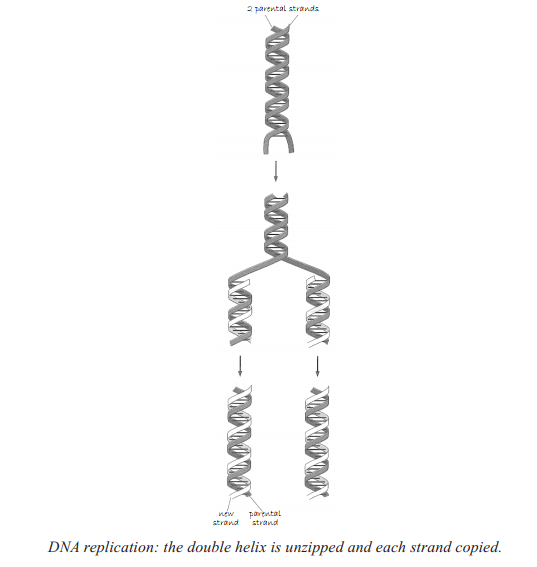
\includegraphics[width=0.75\linewidth]{image/Text5/Fig5.19.png}
\end{figure}

\noindent 58\\
There remained, however, a single missing piece in the double helical jigsaw puzzle: our unzipping idea for DNA replication had yet to be experimentally verified. Max Delbrück, for example, was unconvinced. Though he liked the double helix as a model, he worried that unzipping it might generate horrible knots. Five years later, a former student of Pauling’s, Matt Meselson, and the equally bright young phage worker Frank Stahl put to rest such fears when they published the results of a single elegant experiment.\\
然而,在DNA双螺旋结构这个拼图中仍缺少一块:我们提出的DNA复制时 “解旋” 的观点尚未得到实验验证。例如,马克斯·德尔布吕克就对此表示怀疑。尽管他认可双螺旋模型,但担心解旋过程中可能会产生复杂的纽结。五年后,鲍林以前的学生马特·梅塞尔森,以及同样聪慧的年轻噬菌体研究者弗兰克·斯塔尔,发表了一个巧妙的实验结果,打消了人们的这种担忧。 \\

\noindent 59\\
They had met in the summer of 1954 at the Marine Biological Laboratory at Woods Hole, Massachusetts, where I was then lecturing, and agreed—over a good many gin martinis—that they should get together to do some science. The result of their collaboration has been described as “the most beautiful experiment in biology.”
1954年夏天,他们在马萨诸塞州伍兹霍尔的海洋生物实验室相遇,当时我正在那里讲学。在喝了很多杯杜松子马提尼酒后,他们达成一致,认为应该携手开展一些科学研究。他们合作的成果被称为 “生物学中最精妙的实验”。 \\

\begin{figure}
    \centering
    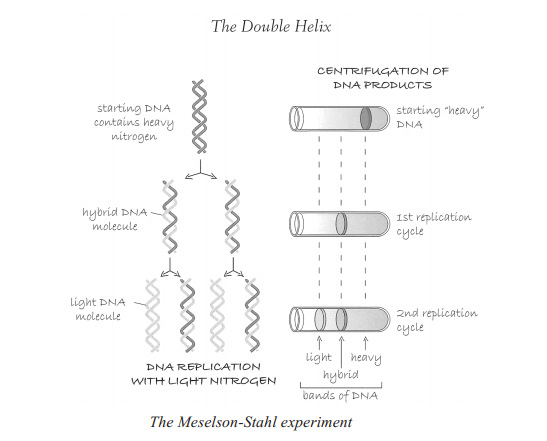
\includegraphics[width=0.75\linewidth]{image/Text5/Fig5.20.png}
\end{figure}

\noindent 60\\
They used a centrifugation technique that allowed them to sort molecules according to slight differences in weight; following a centrifugal spin, heavier molecules end up nearer the bottom of the test tube than lighter ones. Because nitrogen atoms (N) are a component of DNA, and because they exist in two distinct forms, one light and one heavy, Meselson and Stahl were able to tag segments of DNA and thereby track the process of its replication in bacteria. Initially all the bacteria were raised in a medium containing heavy N, which was thus incorporated in both strands of the DNA. From this culture they took a sample, transferring it to a medium containing only light N, ensuring that the next round of DNA replication would have to make use of light N. If, as Crick and I had predicted, DNA replication involves unzipping the double helix and copying each strand, the resultant two “daughter” DNA molecules in the experiment would be hybrids, each consisting of one heavy N strand (the template strand derived from the “parent” molecule) and one light N strand (the one newly fabricated from the new medium). Meselson and Stahl’s centrifugation procedure bore out these expectations precisely. They found three discrete bands in their centrifuge tubes, with the heavy-then-light sample halfway between the heavy-heavy and light-light samples. DNA replication works just as our model supposed it would.\\
他们采用了一种离心技术,该技术能根据分子重量的细微差异对其进行分离;经过离心旋转后,较重的分子会比较轻的分子更靠近试管底部。由于氮原子(N)是DNA的组成成分,且有两种不同的形式,即轻氮和重氮,梅塞尔森和斯塔尔得以标记DNA片段,进而追踪其在细菌中的复制过程。起初,所有细菌都在含有重氮的培养基中培养,因此重氮被整合到了DNA的两条链中。他们从该培养物中取出一份样本,转移到只含轻氮的培养基中,以确保下一轮DNA复制必须使用轻氮。正如我和克里克所预测的那样,如果DNA复制涉及双螺旋解旋以及每条链的复制,那么实验中产生的两个 “子代” DNA分子将是杂合分子,每个子代分子都由一条重氮链(来自 “亲代” 分子的模板链)和一条轻氮链(在新培养基中新合成的链)组成。梅塞尔森和斯塔尔的离心实验结果完全证实了这些预期。他们在离心管中发现了三条清晰的条带,先重后轻的样本条带位于全重样本条带和全轻样本条带的中间位置。DNA的复制过程正如我们的模型所设想的那样。\\ 

\begin{figure}
    \centering
    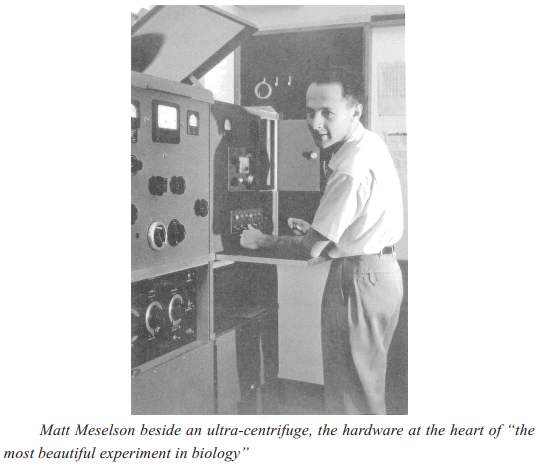
\includegraphics[width=0.75\linewidth]{image/Text5/Fig5.21.png}
\end{figure}

\noindent 61\\
The biochemical nuts and bolts of DNA replication were being analyzed at around the same time in Arthur Kornberg’s laboratory at Washington University in St. Louis. By developing a new, “cell-free” system for DNA synthesis, Kornberg discovered an enzyme (DNA polymerase) that links the DNA components and makes the chemical bonds of the DNA backbone. Kornberg’s enzymatic synthesis of DNA was such an unanticipated and important event that he was awarded the 1959 Nobel Prize in Physiology or Medicine, less than two years after the key experiments. After his prize was announced, Kornberg was photographed holding a copy of the double helix model I had taken to Cold Spring Harbor in 1953.\\
大约在同一时期,圣路易斯华盛顿大学亚瑟·科恩伯格的实验室正在对DNA复制的生物化学基本原理进行分析。科恩伯格通过开发一种新的 “无细胞” DNA合成系统,发现了一种酶(DNA聚合酶),这种酶可以连接DNA的各个组成部分,并形成DNA骨架的化学键。科恩伯格在酶作用下进行的DNA合成是一项出乎意料的重大发现,在关键实验完成后不到两年,他就被授予了1959年诺贝尔生理学或医学奖。在宣布他获奖之后,有人拍到他手持一个我于1953年带到冷泉港的双螺旋结构模型复制品。\\

\noindent 62\\
It was not until 1962 that Francis Crick, Maurice Wilkins, and I were to receive our own Nobel Prize in Physiology or Medicine. Four years earlier, Rosalind Franklin had died of ovarian cancer at the tragically young age of thirty-seven. Before then Crick had become a close colleague and a real friend of Franklin’s. Following the two operations that would fail to stem the advance of her cancer, Franklin convalesced with Crick and his wife, Odile, in Cambridge.\\
直到1962年,弗朗西斯·克里克、莫里斯·威尔金斯和我才获得诺贝尔生理学或医学奖。四年前,罗莎琳德·富兰克林因卵巢癌去世,年仅37岁,令人惋惜。在此之前,克里克已经成为富兰克林亲密的同事和真正的朋友。在两次手术都未能阻止癌细胞扩散后,富兰克林在剑桥与克里克和他的妻子奥迪尔一起疗养。\\ 

\begin{figure}
    \centering
    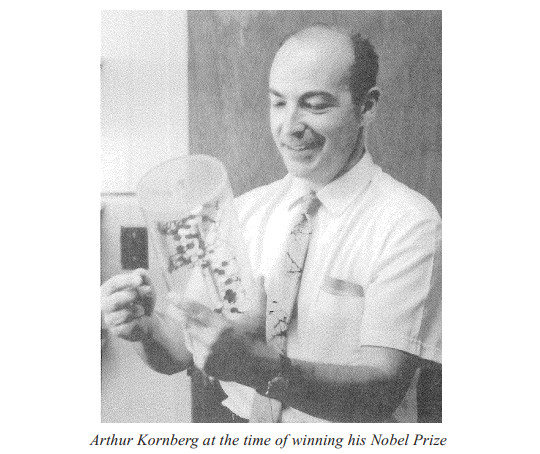
\includegraphics[width=0.75\linewidth]{image/Text5/Fig5.22.png}
\end{figure}

\noindent 63\\
It was and remains a long - standing rule of the Nobel Committee never to split a single prize more than three ways. Had Franklin lived, the problem would have arisen whether to bestow the award upon her or Maurice Wilkins. The Swedes might have resolved the dilemma by awarding them both the Nobel Prize in Chemistry that year. Instead, it went to Max Perutz and John Kendrew, who had elucidated the three - dimensional structures of hemoglobin and myoglobin respectively.\\
一直以来,诺贝尔委员会有个长期不变的规则,即单个奖项的获奖者最多为三人。如果富兰克林还在世,就会出现一个问题,那就是该把这个奖项授予她还是莫里斯·威尔金斯。瑞典人或许会通过在那年同时授予他们诺贝尔化学奖来解决这一困境。然而,该奖项最终授予了马克斯·佩鲁茨和约翰·肯德鲁,他们分别阐明了血红蛋白和肌红蛋白的三维结构。 \\

\noindent 64\\
The discovery of the double helix sounded the death knell for vitalism. Serious scientists, even those religiously inclined, realized that a complete understanding of life would not require the revelation of new laws of nature. Life was just a matter of physics and chemistry, albeit exquisitely organized physics and chemistry. The immediate task ahead would be to figure out how the DNA-encoded script of life went about its work. How does the molecular machinery of cells read the messages of DNA molecules? As the next chapter will reveal, the unexpected complexity of the reading mechanism led to profound insights into how life first came about.\\
DNA双螺旋结构的发现敲响了活力论的丧钟。严谨的科学家,甚至是那些有宗教信仰倾向的科学家,都意识到,要全面理解生命,并不需要揭示新的自然法则。生命仅仅是物理学和化学的问题,尽管是高度有序的物理学和化学。接下来迫在眉睫的任务是弄清楚,由DNA编码的生命 “剧本” 是如何发挥作用的。细胞的分子机制是如何读取DNA分子携带的信息的呢?下一章将会讲到,这一读取机制出乎意料的复杂性,让我们对生命的起源有了深刻的认识。 \\

\newpage

\section{Text 6 from Silent Spring/ \textit{Rachel Carson}}
\newpage
\section{Text 7 from Science and Method/ \textit{Henri Poincaré}}
\newpage
\section{Text 8 from In Search of Memory: The Emergence of a New Science of Mind/ \textit{Eric R. Kandel}}
\newpage
\section{Text 9 from The Shorter Science and Civilisation in China/ \textit{Joseph Needham}}
\newpage
\section{Text 10a from Why the Scientific Revolution Did Not Take Place in China—or Didn’t It?/ \textit{Nathan Sivin}}
\newpage
\section{Text 10b from 《夢溪筆談》/ \textit{沈括} Brush Talks from Dream Brook/ \textit{Shen Kua}}
\newpage
\section{Text 11a from The Mathematical Universe/ \textit{William Dunham}}
\newpage
\section{Text 11b from Elements/ \textit{Euclid}}

\end{document}